\documentclass[twoside]{book}

% Packages required by doxygen
\usepackage{fixltx2e}
\usepackage{calc}
\usepackage{doxygen}
\usepackage[export]{adjustbox} % also loads graphicx
\usepackage{graphicx}
\usepackage[utf8]{inputenc}
\usepackage{makeidx}
\usepackage{multicol}
\usepackage{multirow}
\PassOptionsToPackage{warn}{textcomp}
\usepackage{textcomp}
\usepackage[nointegrals]{wasysym}
\usepackage[table]{xcolor}

% Font selection
\usepackage[T1]{fontenc}
\usepackage[scaled=.90]{helvet}
\usepackage{courier}
\usepackage{amssymb}
\usepackage{sectsty}
\renewcommand{\familydefault}{\sfdefault}
\allsectionsfont{%
  \fontseries{bc}\selectfont%
  \color{darkgray}%
}
\renewcommand{\DoxyLabelFont}{%
  \fontseries{bc}\selectfont%
  \color{darkgray}%
}
\newcommand{\+}{\discretionary{\mbox{\scriptsize$\hookleftarrow$}}{}{}}

% Page & text layout
\usepackage{geometry}
\geometry{%
  a4paper,%
  top=2.5cm,%
  bottom=2.5cm,%
  left=2.5cm,%
  right=2.5cm%
}
\tolerance=750
\hfuzz=15pt
\hbadness=750
\setlength{\emergencystretch}{15pt}
\setlength{\parindent}{0cm}
\setlength{\parskip}{3ex plus 2ex minus 2ex}
\makeatletter
\renewcommand{\paragraph}{%
  \@startsection{paragraph}{4}{0ex}{-1.0ex}{1.0ex}{%
    \normalfont\normalsize\bfseries\SS@parafont%
  }%
}
\renewcommand{\subparagraph}{%
  \@startsection{subparagraph}{5}{0ex}{-1.0ex}{1.0ex}{%
    \normalfont\normalsize\bfseries\SS@subparafont%
  }%
}
\makeatother

% Headers & footers
\usepackage{fancyhdr}
\pagestyle{fancyplain}
\fancyhead[LE]{\fancyplain{}{\bfseries\thepage}}
\fancyhead[CE]{\fancyplain{}{}}
\fancyhead[RE]{\fancyplain{}{\bfseries\leftmark}}
\fancyhead[LO]{\fancyplain{}{\bfseries\rightmark}}
\fancyhead[CO]{\fancyplain{}{}}
\fancyhead[RO]{\fancyplain{}{\bfseries\thepage}}
\fancyfoot[LE]{\fancyplain{}{}}
\fancyfoot[CE]{\fancyplain{}{}}
\fancyfoot[RE]{\fancyplain{}{\bfseries\scriptsize Generated by Doxygen }}
\fancyfoot[LO]{\fancyplain{}{\bfseries\scriptsize Generated by Doxygen }}
\fancyfoot[CO]{\fancyplain{}{}}
\fancyfoot[RO]{\fancyplain{}{}}
\renewcommand{\footrulewidth}{0.4pt}
\renewcommand{\chaptermark}[1]{%
  \markboth{#1}{}%
}
\renewcommand{\sectionmark}[1]{%
  \markright{\thesection\ #1}%
}

% Indices & bibliography
\usepackage{natbib}
\usepackage[titles]{tocloft}
\setcounter{tocdepth}{3}
\setcounter{secnumdepth}{5}
\makeindex

% Hyperlinks (required, but should be loaded last)
\usepackage{ifpdf}
\ifpdf
  \usepackage[pdftex,pagebackref=true]{hyperref}
\else
  \usepackage[ps2pdf,pagebackref=true]{hyperref}
\fi
\hypersetup{%
  colorlinks=true,%
  linkcolor=blue,%
  citecolor=blue,%
  unicode%
}

% Custom commands
\newcommand{\clearemptydoublepage}{%
  \newpage{\pagestyle{empty}\cleardoublepage}%
}

\usepackage{caption}
\captionsetup{labelsep=space,justification=centering,font={bf},singlelinecheck=off,skip=4pt,position=top}

%===== C O N T E N T S =====

\begin{document}

% Titlepage & ToC
\hypersetup{pageanchor=false,
             bookmarksnumbered=true,
             pdfencoding=unicode
            }
\pagenumbering{roman}
\begin{titlepage}
\vspace*{7cm}
\begin{center}%
{\Large Omicron $\vert$ A\+PI \\[1ex]\large Version 0.\+0.\+1 }\\
\vspace*{1cm}
{\large Generated by Doxygen 1.8.11}\\
\end{center}
\end{titlepage}
\clearemptydoublepage
\tableofcontents
\clearemptydoublepage
\pagenumbering{arabic}
\hypersetup{pageanchor=true}

%--- Begin generated contents ---
\chapter{Todo List}
\label{todo}
\hypertarget{todo}{}

\begin{DoxyRefList}
\item[\label{todo__todo000001}%
\hypertarget{todo__todo000001}{}%
Class \hyperlink{classomi_1_1asset_1_1_asset_library}{omi\+:\+:asset\+:\+:Asset\+Library} ]
\end{DoxyRefList}
\chapter{Namespace Index}
\section{Namespace List}
Here is a list of all documented namespaces with brief descriptions\+:\begin{DoxyCompactList}
\item\contentsline{section}{\hyperlink{namespaceomi}{omi} \\*The global namespace of the Omicron engine }{\pageref{namespaceomi}}{}
\item\contentsline{section}{\hyperlink{namespaceomi_1_1asset}{omi\+::asset} \\*Module for asset management in Omicron (loading and access of resources) }{\pageref{namespaceomi_1_1asset}}{}
\item\contentsline{section}{\hyperlink{namespaceomi_1_1asset_1_1global}{omi\+::asset\+::global} \\*Globals for Omicron\textquotesingle{}s asset module }{\pageref{namespaceomi_1_1asset_1_1global}}{}
\item\contentsline{section}{\hyperlink{namespaceomi_1_1config}{omi\+::config} \\*Module for accessing configuration data through Arcane\+Core Config in Omicron }{\pageref{namespaceomi_1_1config}}{}
\item\contentsline{section}{\hyperlink{namespaceomi_1_1config_1_1global}{omi\+::config\+::global} \\*Globals relating to configuration data though Arcane\+Core Config in Omicron }{\pageref{namespaceomi_1_1config_1_1global}}{}
\item\contentsline{section}{\hyperlink{namespaceomi_1_1render_1_1ss}{omi\+::render\+::ss} \\*Module for implementing Omicron rendering subsystems }{\pageref{namespaceomi_1_1render_1_1ss}}{}
\item\contentsline{section}{\hyperlink{namespaceomi_1_1report}{omi\+::report} \\*Module for reporting logs and diagnostics through Omicron }{\pageref{namespaceomi_1_1report}}{}
\item\contentsline{section}{\hyperlink{namespaceomi_1_1report_1_1global}{omi\+::report\+::global} \\*Globals for Omicron\textquotesingle{}s report module }{\pageref{namespaceomi_1_1report_1_1global}}{}
\item\contentsline{section}{\hyperlink{namespaceomi_1_1runtime}{omi\+::runtime} \\*The global namespace of the private omicron runtime }{\pageref{namespaceomi_1_1runtime}}{}
\item\contentsline{section}{\hyperlink{namespaceomi_1_1runtime_1_1boot}{omi\+::runtime\+::boot} \\*Supplies the routines for startup and shutdown of Omicron }{\pageref{namespaceomi_1_1runtime_1_1boot}}{}
\item\contentsline{section}{\hyperlink{namespaceomi_1_1runtime_1_1global}{omi\+::runtime\+::global} \\*Global objects for the Omicron runtime }{\pageref{namespaceomi_1_1runtime_1_1global}}{}
\item\contentsline{section}{\hyperlink{namespaceomi_1_1runtime_1_1ss}{omi\+::runtime\+::ss} \\*Omicron\textquotesingle{}s subsystem management }{\pageref{namespaceomi_1_1runtime_1_1ss}}{}
\item\contentsline{section}{\hyperlink{namespaceomi_1_1ss}{omi\+::ss} \\*Library for implementing Omicron Subsystems }{\pageref{namespaceomi_1_1ss}}{}
\item\contentsline{section}{\hyperlink{namespaceomi_1_1window}{omi\+::window} \\*The window management interface of Omicron }{\pageref{namespaceomi_1_1window}}{}
\item\contentsline{section}{\hyperlink{namespaceomi_1_1window_1_1ss}{omi\+::window\+::ss} \\*Module for implementing Omicron window subsystems }{\pageref{namespaceomi_1_1window_1_1ss}}{}
\end{DoxyCompactList}

\chapter{Hierarchical Index}
\section{Class Hierarchy}
This inheritance list is sorted roughly, but not completely, alphabetically\+:\begin{DoxyCompactList}
\item \contentsline{section}{omi\+:\+:runtime\+:\+:Abstract\+Clock}{\pageref{classomi_1_1runtime_1_1_abstract_clock}}{}
\begin{DoxyCompactList}
\item \contentsline{section}{omi\+:\+:runtime\+:\+:Game\+Clock}{\pageref{classomi_1_1runtime_1_1_game_clock}}{}
\item \contentsline{section}{omi\+:\+:runtime\+:\+:Wall\+Clock}{\pageref{classomi_1_1runtime_1_1_wall_clock}}{}
\end{DoxyCompactList}
\end{DoxyCompactList}

\chapter{Class Index}
\section{Class List}
Here are the classes, structs, unions and interfaces with brief descriptions\+:\begin{DoxyCompactList}
\item\contentsline{section}{\hyperlink{classomi_1_1runtime_1_1_abstract_clock}{omi\+::runtime\+::\+Abstract\+Clock} \\*Abstract time keeping device }{\pageref{classomi_1_1runtime_1_1_abstract_clock}}{}
\item\contentsline{section}{\hyperlink{classomi_1_1runtime_1_1_game_clock}{omi\+::runtime\+::\+Game\+Clock} \\*Clock that measures time since the game engine last started }{\pageref{classomi_1_1runtime_1_1_game_clock}}{}
\item\contentsline{section}{\hyperlink{classomi_1_1runtime_1_1_wall_clock}{omi\+::runtime\+::\+Wall\+Clock} \\*Clock that measures real time from January 1st 1970 }{\pageref{classomi_1_1runtime_1_1_wall_clock}}{}
\end{DoxyCompactList}

\chapter{File Index}
\section{File List}
Here is a list of all documented files with brief descriptions\+:\begin{DoxyCompactList}
\item\contentsline{section}{/home/david/\+Dropbox/\+Development/\+Omicron/\+Omicron/src/cpp/builtin\+\_\+subsystems/omi\+\_\+al/\hyperlink{_a_l_subsystem_8hpp}{A\+L\+Subsystem.\+hpp} }{\pageref{_a_l_subsystem_8hpp}}{}
\item\contentsline{section}{/home/david/\+Dropbox/\+Development/\+Omicron/\+Omicron/src/cpp/builtin\+\_\+subsystems/omi\+\_\+bullet/\hyperlink{_bullet_subsystem_8hpp}{Bullet\+Subsystem.\+hpp} }{\pageref{_bullet_subsystem_8hpp}}{}
\item\contentsline{section}{/home/david/\+Dropbox/\+Development/\+Omicron/\+Omicron/src/cpp/builtin\+\_\+subsystems/omi\+\_\+gl/\hyperlink{_g_l_bootstrap_8hpp}{G\+L\+Bootstrap.\+hpp} }{\pageref{_g_l_bootstrap_8hpp}}{}
\item\contentsline{section}{/home/david/\+Dropbox/\+Development/\+Omicron/\+Omicron/src/cpp/builtin\+\_\+subsystems/omi\+\_\+gl/\hyperlink{_g_l_globals_8hpp}{G\+L\+Globals.\+hpp} \\*Globals for Omi GL }{\pageref{_g_l_globals_8hpp}}{}
\item\contentsline{section}{/home/david/\+Dropbox/\+Development/\+Omicron/\+Omicron/src/cpp/builtin\+\_\+subsystems/omi\+\_\+gl/\hyperlink{_g_l_subsystem_8hpp}{G\+L\+Subsystem.\+hpp} }{\pageref{_g_l_subsystem_8hpp}}{}
\item\contentsline{section}{/home/david/\+Dropbox/\+Development/\+Omicron/\+Omicron/src/cpp/builtin\+\_\+subsystems/omi\+\_\+qt/\hyperlink{_qt_bootstrap_8hpp}{Qt\+Bootstrap.\+hpp} }{\pageref{_qt_bootstrap_8hpp}}{}
\item\contentsline{section}{/home/david/\+Dropbox/\+Development/\+Omicron/\+Omicron/src/cpp/builtin\+\_\+subsystems/omi\+\_\+qt/\hyperlink{_qt_globals_8hpp}{Qt\+Globals.\+hpp} \\*Globals for Omi Qt }{\pageref{_qt_globals_8hpp}}{}
\item\contentsline{section}{/home/david/\+Dropbox/\+Development/\+Omicron/\+Omicron/src/cpp/builtin\+\_\+subsystems/omi\+\_\+qt/\hyperlink{_qt_main_window_8hpp}{Qt\+Main\+Window.\+hpp} }{\pageref{_qt_main_window_8hpp}}{}
\item\contentsline{section}{/home/david/\+Dropbox/\+Development/\+Omicron/\+Omicron/src/cpp/builtin\+\_\+subsystems/pxtrace/\hyperlink{_camera_8hpp}{Camera.\+hpp} }{\pageref{_camera_8hpp}}{}
\item\contentsline{section}{/home/david/\+Dropbox/\+Development/\+Omicron/\+Omicron/src/cpp/builtin\+\_\+subsystems/pxtrace/\hyperlink{_frame_buffer_8hpp}{Frame\+Buffer.\+hpp} }{\pageref{_frame_buffer_8hpp}}{}
\item\contentsline{section}{/home/david/\+Dropbox/\+Development/\+Omicron/\+Omicron/src/cpp/builtin\+\_\+subsystems/pxtrace/\hyperlink{_p_x_globals_8hpp}{P\+X\+Globals.\+hpp} \\*Globals for pxtrace }{\pageref{_p_x_globals_8hpp}}{}
\item\contentsline{section}{/home/david/\+Dropbox/\+Development/\+Omicron/\+Omicron/src/cpp/builtin\+\_\+subsystems/pxtrace/\hyperlink{_p_x_subsystem_8hpp}{P\+X\+Subsystem.\+hpp} }{\pageref{_p_x_subsystem_8hpp}}{}
\item\contentsline{section}{/home/david/\+Dropbox/\+Development/\+Omicron/\+Omicron/src/cpp/builtin\+\_\+subsystems/pxtrace/\hyperlink{_sphere_8hpp}{Sphere.\+hpp} }{\pageref{_sphere_8hpp}}{}
\item\contentsline{section}{/home/david/\+Dropbox/\+Development/\+Omicron/\+Omicron/src/cpp/omicron/\hyperlink{____omicron_8hpp}{\+\_\+\+\_\+omicron.\+hpp} \\*Documents the omi namespace }{\pageref{____omicron_8hpp}}{}
\item\contentsline{section}{/home/david/\+Dropbox/\+Development/\+Omicron/\+Omicron/src/cpp/omicron/api/\hyperlink{_a_p_i_8hpp}{A\+P\+I.\+hpp} \\*Globals definitions for the Omicron A\+PI }{\pageref{_a_p_i_8hpp}}{}
\item\contentsline{section}{/home/david/\+Dropbox/\+Development/\+Omicron/\+Omicron/src/cpp/omicron/api/asset/\hyperlink{____asset_8hpp}{\+\_\+\+\_\+asset.\+hpp} \\*Documents the \hyperlink{namespaceomi_1_1asset}{omi\+::asset} namespace }{\pageref{____asset_8hpp}}{}
\item\contentsline{section}{/home/david/\+Dropbox/\+Development/\+Omicron/\+Omicron/src/cpp/omicron/api/asset/\hyperlink{_asset_globals_8hpp}{Asset\+Globals.\+hpp} \\*Globals for Omicron\textquotesingle{}s asset module }{\pageref{_asset_globals_8hpp}}{}
\item\contentsline{section}{/home/david/\+Dropbox/\+Development/\+Omicron/\+Omicron/src/cpp/omicron/api/asset/\hyperlink{_asset_library_8hpp}{Asset\+Library.\+hpp} }{\pageref{_asset_library_8hpp}}{}
\item\contentsline{section}{/home/david/\+Dropbox/\+Development/\+Omicron/\+Omicron/src/cpp/omicron/api/asset/\hyperlink{_resource_8hpp}{Resource.\+hpp} }{\pageref{_resource_8hpp}}{}
\item\contentsline{section}{/home/david/\+Dropbox/\+Development/\+Omicron/\+Omicron/src/cpp/omicron/api/asset/resource/\hyperlink{_abstract_resource_8hpp}{Abstract\+Resource.\+hpp} }{\pageref{_abstract_resource_8hpp}}{}
\item\contentsline{section}{/home/david/\+Dropbox/\+Development/\+Omicron/\+Omicron/src/cpp/omicron/api/asset/resource/\hyperlink{_o_b_j_resource_8hpp}{O\+B\+J\+Resource.\+hpp} }{\pageref{_o_b_j_resource_8hpp}}{}
\item\contentsline{section}{/home/david/\+Dropbox/\+Development/\+Omicron/\+Omicron/src/cpp/omicron/api/asset/types/\hyperlink{_abstract_asset_8hpp}{Abstract\+Asset.\+hpp} }{\pageref{_abstract_asset_8hpp}}{}
\item\contentsline{section}{/home/david/\+Dropbox/\+Development/\+Omicron/\+Omicron/src/cpp/omicron/api/asset/types/\hyperlink{_geometry_8hpp}{Geometry.\+hpp} }{\pageref{_geometry_8hpp}}{}
\item\contentsline{section}{/home/david/\+Dropbox/\+Development/\+Omicron/\+Omicron/src/cpp/omicron/api/asset/types/bk/\hyperlink{bk_2_abstract_asset_8hpp}{Abstract\+Asset.\+hpp} }{\pageref{bk_2_abstract_asset_8hpp}}{}
\item\contentsline{section}{/home/david/\+Dropbox/\+Development/\+Omicron/\+Omicron/src/cpp/omicron/api/asset/types/bk/\hyperlink{_compound_asset_8hpp}{Compound\+Asset.\+hpp} }{\pageref{_compound_asset_8hpp}}{}
\item\contentsline{section}{/home/david/\+Dropbox/\+Development/\+Omicron/\+Omicron/src/cpp/omicron/api/asset/types/bk/\hyperlink{_geometry_asset_8hpp}{Geometry\+Asset.\+hpp} }{\pageref{_geometry_asset_8hpp}}{}
\item\contentsline{section}{/home/david/\+Dropbox/\+Development/\+Omicron/\+Omicron/src/cpp/omicron/api/asset/types/bk/\hyperlink{_material_asset_8hpp}{Material\+Asset.\+hpp} }{\pageref{_material_asset_8hpp}}{}
\item\contentsline{section}{/home/david/\+Dropbox/\+Development/\+Omicron/\+Omicron/src/cpp/omicron/api/asset/types/bk/\hyperlink{_mesh_asset_8hpp}{Mesh\+Asset.\+hpp} }{\pageref{_mesh_asset_8hpp}}{}
\item\contentsline{section}{/home/david/\+Dropbox/\+Development/\+Omicron/\+Omicron/src/cpp/omicron/api/asset/types/bk/\hyperlink{_shader_asset_8hpp}{Shader\+Asset.\+hpp} }{\pageref{_shader_asset_8hpp}}{}
\item\contentsline{section}{/home/david/\+Dropbox/\+Development/\+Omicron/\+Omicron/src/cpp/omicron/api/asset/types/bk/\hyperlink{_texture_asset_8hpp}{Texture\+Asset.\+hpp} }{\pageref{_texture_asset_8hpp}}{}
\item\contentsline{section}{/home/david/\+Dropbox/\+Development/\+Omicron/\+Omicron/src/cpp/omicron/api/asset/types/bk/\hyperlink{_vertex_attributes_asset_8hpp}{Vertex\+Attributes\+Asset.\+hpp} }{\pageref{_vertex_attributes_asset_8hpp}}{}
\item\contentsline{section}{/home/david/\+Dropbox/\+Development/\+Omicron/\+Omicron/src/cpp/omicron/api/common/attribute/\hyperlink{_attribute_8hpp}{Attribute.\+hpp} }{\pageref{_attribute_8hpp}}{}
\item\contentsline{section}{/home/david/\+Dropbox/\+Development/\+Omicron/\+Omicron/src/cpp/omicron/api/common/attribute/\hyperlink{_data_attribute_8hpp}{Data\+Attribute.\+hpp} }{\pageref{_data_attribute_8hpp}}{}
\item\contentsline{section}{/home/david/\+Dropbox/\+Development/\+Omicron/\+Omicron/src/cpp/omicron/api/common/attribute/\hyperlink{_int32_attribute_8hpp}{Int32\+Attribute.\+hpp} }{\pageref{_int32_attribute_8hpp}}{}
\item\contentsline{section}{/home/david/\+Dropbox/\+Development/\+Omicron/\+Omicron/src/cpp/omicron/api/common/attribute/\hyperlink{_map_attribute_8hpp}{Map\+Attribute.\+hpp} }{\pageref{_map_attribute_8hpp}}{}
\item\contentsline{section}{/home/david/\+Dropbox/\+Development/\+Omicron/\+Omicron/src/cpp/omicron/api/config/\hyperlink{____config_8hpp}{\+\_\+\+\_\+config.\+hpp} \\*Documents the \hyperlink{namespaceomi_1_1config}{omi\+::config} namespace }{\pageref{____config_8hpp}}{}
\item\contentsline{section}{/home/david/\+Dropbox/\+Development/\+Omicron/\+Omicron/src/cpp/omicron/api/config/\hyperlink{_config_globals_8hpp}{Config\+Globals.\+hpp} \\*Globals relating to configuration data through Arcane\+Core Config in Omicron }{\pageref{_config_globals_8hpp}}{}
\item\contentsline{section}{/home/david/\+Dropbox/\+Development/\+Omicron/\+Omicron/src/cpp/omicron/api/config/\hyperlink{_config_inline_8hpp}{Config\+Inline.\+hpp} \\*File which is programmitcally generated to provide access to the contents of in memory Arcane\+Core Config data for the Omicron Runtime }{\pageref{_config_inline_8hpp}}{}
\item\contentsline{section}{/home/david/\+Dropbox/\+Development/\+Omicron/\+Omicron/src/cpp/omicron/api/render/subsystem/\hyperlink{_render_bootstrap_8hpp}{Render\+Bootstrap.\+hpp} }{\pageref{_render_bootstrap_8hpp}}{}
\item\contentsline{section}{/home/david/\+Dropbox/\+Development/\+Omicron/\+Omicron/src/cpp/omicron/api/render/subsystem/\hyperlink{_render_interface_8hpp}{Render\+Interface.\+hpp} \\*The interface for registering a rendering subsystem }{\pageref{_render_interface_8hpp}}{}
\item\contentsline{section}{/home/david/\+Dropbox/\+Development/\+Omicron/\+Omicron/src/cpp/omicron/api/report/\hyperlink{____report_8hpp}{\+\_\+\+\_\+report.\+hpp} \\*Documents the \hyperlink{namespaceomi_1_1report}{omi\+::report} namespace }{\pageref{____report_8hpp}}{}
\item\contentsline{section}{/home/david/\+Dropbox/\+Development/\+Omicron/\+Omicron/src/cpp/omicron/api/report/\hyperlink{_logging_8hpp}{Logging.\+hpp} \\*Functionality related to logging through Omicron using Arcane\+Core Log }{\pageref{_logging_8hpp}}{}
\item\contentsline{section}{/home/david/\+Dropbox/\+Development/\+Omicron/\+Omicron/src/cpp/omicron/api/report/{\bfseries Report\+Boot.\+hpp} }{\pageref{_report_boot_8hpp}}{}
\item\contentsline{section}{/home/david/\+Dropbox/\+Development/\+Omicron/\+Omicron/src/cpp/omicron/api/report/\hyperlink{_report_globals_8hpp}{Report\+Globals.\+hpp} \\*Globals for Omicron\textquotesingle{}s report module }{\pageref{_report_globals_8hpp}}{}
\item\contentsline{section}{/home/david/\+Dropbox/\+Development/\+Omicron/\+Omicron/src/cpp/omicron/api/window/\hyperlink{_main_window_8hpp}{Main\+Window.\+hpp} }{\pageref{_main_window_8hpp}}{}
\item\contentsline{section}{/home/david/\+Dropbox/\+Development/\+Omicron/\+Omicron/src/cpp/omicron/api/window/\hyperlink{_window_8hpp}{Window.\+hpp} \\*The global definitions for the Omicron window interface }{\pageref{_window_8hpp}}{}
\item\contentsline{section}{/home/david/\+Dropbox/\+Development/\+Omicron/\+Omicron/src/cpp/omicron/api/window/subsystem/\hyperlink{_window_bootstrap_8hpp}{Window\+Bootstrap.\+hpp} }{\pageref{_window_bootstrap_8hpp}}{}
\item\contentsline{section}{/home/david/\+Dropbox/\+Development/\+Omicron/\+Omicron/src/cpp/omicron/api/window/subsystem/\hyperlink{_window_interface_8hpp}{Window\+Interface.\+hpp} \\*The interface for registering a window subsystem }{\pageref{_window_interface_8hpp}}{}
\item\contentsline{section}{/home/david/\+Dropbox/\+Development/\+Omicron/\+Omicron/src/cpp/omicron/api/xform/\hyperlink{_abstract_constraint_8hpp}{Abstract\+Constraint.\+hpp} }{\pageref{_abstract_constraint_8hpp}}{}
\item\contentsline{section}{/home/david/\+Dropbox/\+Development/\+Omicron/\+Omicron/src/cpp/omicron/api/xform/\hyperlink{_abstract_transform_8hpp}{Abstract\+Transform.\+hpp} }{\pageref{_abstract_transform_8hpp}}{}
\item\contentsline{section}{/home/david/\+Dropbox/\+Development/\+Omicron/\+Omicron/src/cpp/omicron/api/xform/\hyperlink{_hierarchical_constraint_8hpp}{Hierarchical\+Constraint.\+hpp} }{\pageref{_hierarchical_constraint_8hpp}}{}
\item\contentsline{section}{/home/david/\+Dropbox/\+Development/\+Omicron/\+Omicron/src/cpp/omicron/api/xform/\hyperlink{_matrix_8hpp}{Matrix.\+hpp} }{\pageref{_matrix_8hpp}}{}
\item\contentsline{section}{/home/david/\+Dropbox/\+Development/\+Omicron/\+Omicron/src/cpp/omicron/api/xform/\hyperlink{_s_q_t_8hpp}{S\+Q\+T.\+hpp} }{\pageref{_s_q_t_8hpp}}{}
\item\contentsline{section}{/home/david/\+Dropbox/\+Development/\+Omicron/\+Omicron/src/cpp/omicron/api/xform/\hyperlink{_s_r_t_8hpp}{S\+R\+T.\+hpp} }{\pageref{_s_r_t_8hpp}}{}
\item\contentsline{section}{/home/david/\+Dropbox/\+Development/\+Omicron/\+Omicron/src/cpp/omicron/runtime/\hyperlink{____runtime_8hpp}{\+\_\+\+\_\+runtime.\+hpp} \\*Documents the \hyperlink{namespaceomi_1_1runtime}{omi\+::runtime} namespace }{\pageref{____runtime_8hpp}}{}
\item\contentsline{section}{/home/david/\+Dropbox/\+Development/\+Omicron/\+Omicron/src/cpp/omicron/runtime/\hyperlink{_engine_8hpp}{Engine.\+hpp} }{\pageref{_engine_8hpp}}{}
\item\contentsline{section}{/home/david/\+Dropbox/\+Development/\+Omicron/\+Omicron/src/cpp/omicron/runtime/\hyperlink{_runtime_globals_8hpp}{Runtime\+Globals.\+hpp} \\*Globals for the Omicron runtime }{\pageref{_runtime_globals_8hpp}}{}
\item\contentsline{section}{/home/david/\+Dropbox/\+Development/\+Omicron/\+Omicron/src/cpp/omicron/runtime/boot/\hyperlink{____boot_8hpp}{\+\_\+\+\_\+boot.\+hpp} \\*Documents the \hyperlink{namespaceomi_1_1runtime_1_1boot}{omi\+::runtime\+::boot} namespace }{\pageref{____boot_8hpp}}{}
\item\contentsline{section}{/home/david/\+Dropbox/\+Development/\+Omicron/\+Omicron/src/cpp/omicron/runtime/boot/\hyperlink{_boot_logging_8hpp}{Boot\+Logging.\+hpp} \\*Provides the routines for starting and shutting down Omicron runtime logging }{\pageref{_boot_logging_8hpp}}{}
\item\contentsline{section}{/home/david/\+Dropbox/\+Development/\+Omicron/\+Omicron/src/cpp/omicron/runtime/boot/\hyperlink{_boot_routines_8hpp}{Boot\+Routines.\+hpp} \\*Provides the main routines for startup and shutdown of the Omicron }{\pageref{_boot_routines_8hpp}}{}
\item\contentsline{section}{/home/david/\+Dropbox/\+Development/\+Omicron/\+Omicron/src/cpp/omicron/runtime/subsystem/\hyperlink{runtime_2subsystem_2____subsystem_8hpp}{\+\_\+\+\_\+subsystem.\+hpp} \\*Documents the \hyperlink{namespaceomi_1_1runtime_1_1ss}{omi\+::runtime\+::ss} namespace }{\pageref{runtime_2subsystem_2____subsystem_8hpp}}{}
\item\contentsline{section}{/home/david/\+Dropbox/\+Development/\+Omicron/\+Omicron/src/cpp/omicron/runtime/subsystem/\hyperlink{_abstract_subsystem_8hpp}{Abstract\+Subsystem.\+hpp} }{\pageref{_abstract_subsystem_8hpp}}{}
\item\contentsline{section}{/home/david/\+Dropbox/\+Development/\+Omicron/\+Omicron/src/cpp/omicron/runtime/subsystem/\hyperlink{_subsystem_manager_8hpp}{Subsystem\+Manager.\+hpp} }{\pageref{_subsystem_manager_8hpp}}{}
\item\contentsline{section}{/home/david/\+Dropbox/\+Development/\+Omicron/\+Omicron/src/cpp/omicron/runtime/subsystem/\hyperlink{_window_subsystem_8hpp}{Window\+Subsystem.\+hpp} }{\pageref{_window_subsystem_8hpp}}{}
\item\contentsline{section}{/home/david/\+Dropbox/\+Development/\+Omicron/\+Omicron/src/cpp/omicron/subsystem/\hyperlink{subsystem_2____subsystem_8hpp}{\+\_\+\+\_\+subsystem.\+hpp} \\*Documents the \hyperlink{namespaceomi_1_1ss}{omi\+::ss} namespace }{\pageref{subsystem_2____subsystem_8hpp}}{}
\item\contentsline{section}{/home/david/\+Dropbox/\+Development/\+Omicron/\+Omicron/src/cpp/omicron/subsystem/\hyperlink{_audio_8hpp}{Audio.\+hpp} }{\pageref{_audio_8hpp}}{}
\item\contentsline{section}{/home/david/\+Dropbox/\+Development/\+Omicron/\+Omicron/src/cpp/omicron/subsystem/\hyperlink{_input_8hpp}{Input.\+hpp} }{\pageref{_input_8hpp}}{}
\item\contentsline{section}{/home/david/\+Dropbox/\+Development/\+Omicron/\+Omicron/src/cpp/omicron/subsystem/\hyperlink{_physics_8hpp}{Physics.\+hpp} }{\pageref{_physics_8hpp}}{}
\item\contentsline{section}{/home/david/\+Dropbox/\+Development/\+Omicron/\+Omicron/src/cpp/omicron/subsystem/\hyperlink{_renderer_8hpp}{Renderer.\+hpp} }{\pageref{_renderer_8hpp}}{}
\item\contentsline{section}{/home/david/\+Dropbox/\+Development/\+Omicron/\+Omicron/src/cpp/omicron/subsystem/\hyperlink{_subsystem_8hpp}{Subsystem.\+hpp} }{\pageref{_subsystem_8hpp}}{}
\item\contentsline{section}{/home/david/\+Dropbox/\+Development/\+Omicron/\+Omicron/src/cpp/omicron/subsystem/\hyperlink{_u_i_8hpp}{U\+I.\+hpp} }{\pageref{_u_i_8hpp}}{}
\item\contentsline{section}{/home/david/\+Dropbox/\+Development/\+Omicron/\+Omicron/src/cpp/omicron/subsystem/\hyperlink{_window_manager_8hpp}{Window\+Manager.\+hpp} }{\pageref{_window_manager_8hpp}}{}
\end{DoxyCompactList}

\chapter{Namespace Documentation}
\hypertarget{namespaceomi}{}\section{omi Namespace Reference}
\label{namespaceomi}\index{omi@{omi}}


The global namespace of the Omicron engine.  


\subsection*{Namespaces}
\begin{DoxyCompactItemize}
\item 
 \hyperlink{namespaceomi_1_1runtime}{runtime}
\begin{DoxyCompactList}\small\item\em The runtime management aspects of the Omicron engine. \end{DoxyCompactList}\end{DoxyCompactItemize}


\subsection{Detailed Description}
The global namespace of the Omicron engine. 
\hypertarget{namespaceomi_1_1asset}{}\section{omi\+:\+:asset Namespace Reference}
\label{namespaceomi_1_1asset}\index{omi\+::asset@{omi\+::asset}}


Module for asset management in Omicron (loading and access of resources).  


\subsection*{Namespaces}
\begin{DoxyCompactItemize}
\item 
 \hyperlink{namespaceomi_1_1asset_1_1global}{global}
\begin{DoxyCompactList}\small\item\em Globals for Omicron\textquotesingle{}s asset module. \end{DoxyCompactList}\end{DoxyCompactItemize}
\subsection*{Classes}
\begin{DoxyCompactItemize}
\item 
class \hyperlink{classomi_1_1asset_1_1_abstract_asset}{Abstract\+Asset}
\item 
class \hyperlink{classomi_1_1asset_1_1_abstract_resource}{Abstract\+Resource}
\item 
class \hyperlink{classomi_1_1asset_1_1_asset_library}{Asset\+Library}
\begin{DoxyCompactList}\small\item\em Singleton object which is used to load, store, provide access to, and release game resources. \end{DoxyCompactList}\item 
class \hyperlink{classomi_1_1asset_1_1_geometry}{Geometry}
\item 
class \hyperlink{classomi_1_1asset_1_1_material}{Material}
\item 
class \hyperlink{classomi_1_1asset_1_1_mesh}{Mesh}
\item 
class \hyperlink{classomi_1_1asset_1_1_o_b_j_resource}{O\+B\+J\+Resource}
\item 
class \hyperlink{classomi_1_1asset_1_1_shader}{Shader}
\item 
class \hyperlink{classomi_1_1asset_1_1_texture}{Texture}
\item 
class \hyperlink{classomi_1_1asset_1_1_vertex_attributes}{Vertex\+Attributes}
\end{DoxyCompactItemize}


\subsection{Detailed Description}
Module for asset management in Omicron (loading and access of resources). 
\hypertarget{namespaceomi_1_1asset_1_1global}{}\section{omi\+:\+:asset\+:\+:global Namespace Reference}
\label{namespaceomi_1_1asset_1_1global}\index{omi\+::asset\+::global@{omi\+::asset\+::global}}


Globals for Omicron\textquotesingle{}s asset module.  


\subsection*{Variables}
\begin{DoxyCompactItemize}
\item 
arc\+::log\+::\+Input $\ast$ \hyperlink{namespaceomi_1_1asset_1_1global_ae52188e7280eea518c79cc6bebf7de6e}{logger}\hypertarget{namespaceomi_1_1asset_1_1global_ae52188e7280eea518c79cc6bebf7de6e}{}\label{namespaceomi_1_1asset_1_1global_ae52188e7280eea518c79cc6bebf7de6e}

\begin{DoxyCompactList}\small\item\em The logging input to be used by the Omicron asset system. \end{DoxyCompactList}\item 
const arc\+::io\+::sys\+::\+Path \hyperlink{namespaceomi_1_1asset_1_1global_a99d9deb4d764e55094411b9c1f760a3e}{config\+\_\+root\+\_\+dir}\hypertarget{namespaceomi_1_1asset_1_1global_a99d9deb4d764e55094411b9c1f760a3e}{}\label{namespaceomi_1_1asset_1_1global_a99d9deb4d764e55094411b9c1f760a3e}

\begin{DoxyCompactList}\small\item\em The root directory where all Omicron\textquotesingle{}s asset configuration data is located within. \end{DoxyCompactList}\end{DoxyCompactItemize}


\subsection{Detailed Description}
Globals for Omicron\textquotesingle{}s asset module. 
\hypertarget{namespaceomi_1_1config}{}\section{omi\+:\+:config Namespace Reference}
\label{namespaceomi_1_1config}\index{omi\+::config@{omi\+::config}}


Module for accessing configuration data through Arcane\+Core Config in Omicron.  


\subsection*{Namespaces}
\begin{DoxyCompactItemize}
\item 
 \hyperlink{namespaceomi_1_1config_1_1global}{global}
\begin{DoxyCompactList}\small\item\em Globals relating to configuration data though Arcane\+Core Config in Omicron. \end{DoxyCompactList}\end{DoxyCompactItemize}


\subsection{Detailed Description}
Module for accessing configuration data through Arcane\+Core Config in Omicron. 
\hypertarget{namespaceomi_1_1config_1_1global}{}\section{omi\+:\+:config\+:\+:global Namespace Reference}
\label{namespaceomi_1_1config_1_1global}\index{omi\+::config\+::global@{omi\+::config\+::global}}


Globals relating to configuration data though Arcane\+Core Config in Omicron.  


\subsection*{Variables}
\begin{DoxyCompactItemize}
\item 
O\+M\+I\+\_\+\+A\+P\+I\+\_\+\+G\+L\+O\+B\+AL const arc\+::io\+::sys\+::\+Path \hyperlink{namespaceomi_1_1config_1_1global_a08c648c90660a7f22c9a1d4bc19b517d}{root\+\_\+dir}\hypertarget{namespaceomi_1_1config_1_1global_a08c648c90660a7f22c9a1d4bc19b517d}{}\label{namespaceomi_1_1config_1_1global_a08c648c90660a7f22c9a1d4bc19b517d}

\begin{DoxyCompactList}\small\item\em The root directory where all Omicron config data is located within. \end{DoxyCompactList}\end{DoxyCompactItemize}


\subsection{Detailed Description}
Globals relating to configuration data though Arcane\+Core Config in Omicron. 
\hypertarget{namespaceomi_1_1render_1_1ss}{}\section{omi\+:\+:render\+:\+:ss Namespace Reference}
\label{namespaceomi_1_1render_1_1ss}\index{omi\+::render\+::ss@{omi\+::render\+::ss}}


Module for implementing Omicron rendering subsystems.  


\subsection*{Classes}
\begin{DoxyCompactItemize}
\item 
class \hyperlink{classomi_1_1render_1_1ss_1_1_bootstrap}{Bootstrap}
\begin{DoxyCompactList}\small\item\em Object used to bootstrap a rendering subsystem. \end{DoxyCompactList}\end{DoxyCompactItemize}


\subsection{Detailed Description}
Module for implementing Omicron rendering subsystems. 
\hypertarget{namespaceomi_1_1report}{}\section{omi\+:\+:report Namespace Reference}
\label{namespaceomi_1_1report}\index{omi\+::report@{omi\+::report}}


Module for reporting logs and diagnostics through Omicron.  


\subsection*{Namespaces}
\begin{DoxyCompactItemize}
\item 
 \hyperlink{namespaceomi_1_1report_1_1global}{global}
\begin{DoxyCompactList}\small\item\em Globals for Omicron\textquotesingle{}s report module. \end{DoxyCompactList}\end{DoxyCompactItemize}
\subsection*{Functions}
\begin{DoxyCompactItemize}
\item 
void \hyperlink{namespaceomi_1_1report_a81005ec8dedc387f73bf5f6cca89891b}{logging\+\_\+startup\+\_\+routine} ()\hypertarget{namespaceomi_1_1report_a81005ec8dedc387f73bf5f6cca89891b}{}\label{namespaceomi_1_1report_a81005ec8dedc387f73bf5f6cca89891b}

\begin{DoxyCompactList}\small\item\em Initialises the logging component of the report module. \end{DoxyCompactList}\end{DoxyCompactItemize}
\subsection*{Variables}
\begin{DoxyCompactItemize}
\item 
O\+M\+I\+\_\+\+A\+P\+I\+\_\+\+G\+L\+O\+B\+AL arc\+::log\+::\+Log\+Handler \hyperlink{namespaceomi_1_1report_a4f7843447250d0b260bdb3f964faa027}{log\+\_\+handler}\hypertarget{namespaceomi_1_1report_a4f7843447250d0b260bdb3f964faa027}{}\label{namespaceomi_1_1report_a4f7843447250d0b260bdb3f964faa027}

\begin{DoxyCompactList}\small\item\em The global log handler for all Omicron logging. \end{DoxyCompactList}\end{DoxyCompactItemize}


\subsection{Detailed Description}
Module for reporting logs and diagnostics through Omicron. 
\hypertarget{namespaceomi_1_1report_1_1global}{}\section{omi\+:\+:report\+:\+:global Namespace Reference}
\label{namespaceomi_1_1report_1_1global}\index{omi\+::report\+::global@{omi\+::report\+::global}}


Globals for Omicron\textquotesingle{}s report module.  


\subsection*{Variables}
\begin{DoxyCompactItemize}
\item 
const arc\+::io\+::sys\+::\+Path \hyperlink{namespaceomi_1_1report_1_1global_ad36ec5a81ec6a2679f38edff8ef31d9e}{config\+\_\+root\+\_\+dir}\hypertarget{namespaceomi_1_1report_1_1global_ad36ec5a81ec6a2679f38edff8ef31d9e}{}\label{namespaceomi_1_1report_1_1global_ad36ec5a81ec6a2679f38edff8ef31d9e}

\begin{DoxyCompactList}\small\item\em The root directory where all Omicron\textquotesingle{}s report configuration data is located within. \end{DoxyCompactList}\item 
const arc\+::io\+::sys\+::\+Path \hyperlink{namespaceomi_1_1report_1_1global_a994f26dcbffa9c6116621071d7425360}{config\+\_\+logging\+\_\+dir}\hypertarget{namespaceomi_1_1report_1_1global_a994f26dcbffa9c6116621071d7425360}{}\label{namespaceomi_1_1report_1_1global_a994f26dcbffa9c6116621071d7425360}

\begin{DoxyCompactList}\small\item\em The directory where Omicron\textquotesingle{}s logging configuration data is located within. \end{DoxyCompactList}\end{DoxyCompactItemize}


\subsection{Detailed Description}
Globals for Omicron\textquotesingle{}s report module. 
\hypertarget{namespaceomi_1_1runtime}{}\section{omi\+:\+:runtime Namespace Reference}
\label{namespaceomi_1_1runtime}\index{omi\+::runtime@{omi\+::runtime}}


The global namespace of the private omicron runtime.  


\subsection*{Namespaces}
\begin{DoxyCompactItemize}
\item 
 \hyperlink{namespaceomi_1_1runtime_1_1boot}{boot}
\begin{DoxyCompactList}\small\item\em Supplies the routines for startup and shutdown of Omicron. \end{DoxyCompactList}\item 
 \hyperlink{namespaceomi_1_1runtime_1_1global}{global}
\begin{DoxyCompactList}\small\item\em Global objects for the Omicron runtime. \end{DoxyCompactList}\item 
 \hyperlink{namespaceomi_1_1runtime_1_1ss}{ss}
\begin{DoxyCompactList}\small\item\em Omicron\textquotesingle{}s subsystem management. \end{DoxyCompactList}\end{DoxyCompactItemize}
\subsection*{Classes}
\begin{DoxyCompactItemize}
\item 
class \hyperlink{classomi_1_1runtime_1_1_engine}{Engine}
\begin{DoxyCompactList}\small\item\em Singleton object that owns and starts the Omicron runtime. \end{DoxyCompactList}\end{DoxyCompactItemize}


\subsection{Detailed Description}
The global namespace of the private omicron runtime. 
\hypertarget{namespaceomi_1_1runtime_1_1boot}{}\section{omi\+:\+:runtime\+:\+:boot Namespace Reference}
\label{namespaceomi_1_1runtime_1_1boot}\index{omi\+::runtime\+::boot@{omi\+::runtime\+::boot}}


Supplies the routines for startup and shutdown of Omicron.  


\subsection*{Functions}
\begin{DoxyCompactItemize}
\item 
bool \hyperlink{namespaceomi_1_1runtime_1_1boot_ae5727a38c5b2a13151d32cc9bc8d6989}{startup\+\_\+logging\+\_\+subroutine} ()
\begin{DoxyCompactList}\small\item\em Performs the startup subroutine for Omicron runtime logging. \end{DoxyCompactList}\item 
bool \hyperlink{namespaceomi_1_1runtime_1_1boot_aaa8fe999da953495d7cfaba35c1e6fe6}{shutdown\+\_\+logging\+\_\+subroutine} ()
\begin{DoxyCompactList}\small\item\em Performs the shutdown subroutine for Omicron runtime logging. \end{DoxyCompactList}\item 
bool \hyperlink{namespaceomi_1_1runtime_1_1boot_a91590fccb2aaf380d4fee8613334b84c}{startup\+\_\+routine} ()
\begin{DoxyCompactList}\small\item\em Performs the startup subroutines of Omicron. \end{DoxyCompactList}\item 
bool \hyperlink{namespaceomi_1_1runtime_1_1boot_a0b84d982ce5c250bc76b6aa05a574785}{shutdown\+\_\+routine} ()
\begin{DoxyCompactList}\small\item\em Performs the shutdown subroutines of Omicron. \end{DoxyCompactList}\item 
std\+::ostream \& \hyperlink{namespaceomi_1_1runtime_1_1boot_ad16d09079350024024106889c66ae886}{get\+\_\+critical\+\_\+stream} ()
\begin{DoxyCompactList}\small\item\em Returns the output stream that should be used to log critical messages to. \end{DoxyCompactList}\end{DoxyCompactItemize}


\subsection{Detailed Description}
Supplies the routines for startup and shutdown of Omicron. 

\subsection{Function Documentation}
\index{omi\+::runtime\+::boot@{omi\+::runtime\+::boot}!startup\+\_\+logging\+\_\+subroutine@{startup\+\_\+logging\+\_\+subroutine}}
\index{startup\+\_\+logging\+\_\+subroutine@{startup\+\_\+logging\+\_\+subroutine}!omi\+::runtime\+::boot@{omi\+::runtime\+::boot}}
\subsubsection[{\texorpdfstring{startup\+\_\+logging\+\_\+subroutine()}{startup_logging_subroutine()}}]{\setlength{\rightskip}{0pt plus 5cm}bool omi\+::runtime\+::boot\+::startup\+\_\+logging\+\_\+subroutine (
\begin{DoxyParamCaption}
{}
\end{DoxyParamCaption}
)}\hypertarget{namespaceomi_1_1runtime_1_1boot_ae5727a38c5b2a13151d32cc9bc8d6989}{}\label{namespaceomi_1_1runtime_1_1boot_ae5727a38c5b2a13151d32cc9bc8d6989}


Performs the startup subroutine for Omicron runtime logging. 

\begin{DoxyReturn}{Returns}
Whether startup completed successfully. 
\end{DoxyReturn}
\index{omi\+::runtime\+::boot@{omi\+::runtime\+::boot}!shutdown\+\_\+logging\+\_\+subroutine@{shutdown\+\_\+logging\+\_\+subroutine}}
\index{shutdown\+\_\+logging\+\_\+subroutine@{shutdown\+\_\+logging\+\_\+subroutine}!omi\+::runtime\+::boot@{omi\+::runtime\+::boot}}
\subsubsection[{\texorpdfstring{shutdown\+\_\+logging\+\_\+subroutine()}{shutdown_logging_subroutine()}}]{\setlength{\rightskip}{0pt plus 5cm}bool omi\+::runtime\+::boot\+::shutdown\+\_\+logging\+\_\+subroutine (
\begin{DoxyParamCaption}
{}
\end{DoxyParamCaption}
)}\hypertarget{namespaceomi_1_1runtime_1_1boot_aaa8fe999da953495d7cfaba35c1e6fe6}{}\label{namespaceomi_1_1runtime_1_1boot_aaa8fe999da953495d7cfaba35c1e6fe6}


Performs the shutdown subroutine for Omicron runtime logging. 

\begin{DoxyReturn}{Returns}
Whether shutdown completed successfully. 
\end{DoxyReturn}
\index{omi\+::runtime\+::boot@{omi\+::runtime\+::boot}!startup\+\_\+routine@{startup\+\_\+routine}}
\index{startup\+\_\+routine@{startup\+\_\+routine}!omi\+::runtime\+::boot@{omi\+::runtime\+::boot}}
\subsubsection[{\texorpdfstring{startup\+\_\+routine()}{startup_routine()}}]{\setlength{\rightskip}{0pt plus 5cm}bool omi\+::runtime\+::boot\+::startup\+\_\+routine (
\begin{DoxyParamCaption}
{}
\end{DoxyParamCaption}
)}\hypertarget{namespaceomi_1_1runtime_1_1boot_a91590fccb2aaf380d4fee8613334b84c}{}\label{namespaceomi_1_1runtime_1_1boot_a91590fccb2aaf380d4fee8613334b84c}


Performs the startup subroutines of Omicron. 

\begin{DoxyReturn}{Returns}
Whether startup completed successfully. 
\end{DoxyReturn}
\index{omi\+::runtime\+::boot@{omi\+::runtime\+::boot}!shutdown\+\_\+routine@{shutdown\+\_\+routine}}
\index{shutdown\+\_\+routine@{shutdown\+\_\+routine}!omi\+::runtime\+::boot@{omi\+::runtime\+::boot}}
\subsubsection[{\texorpdfstring{shutdown\+\_\+routine()}{shutdown_routine()}}]{\setlength{\rightskip}{0pt plus 5cm}bool omi\+::runtime\+::boot\+::shutdown\+\_\+routine (
\begin{DoxyParamCaption}
{}
\end{DoxyParamCaption}
)}\hypertarget{namespaceomi_1_1runtime_1_1boot_a0b84d982ce5c250bc76b6aa05a574785}{}\label{namespaceomi_1_1runtime_1_1boot_a0b84d982ce5c250bc76b6aa05a574785}


Performs the shutdown subroutines of Omicron. 

\begin{DoxyReturn}{Returns}
Whether shutdown completed successfully. 
\end{DoxyReturn}
\index{omi\+::runtime\+::boot@{omi\+::runtime\+::boot}!get\+\_\+critical\+\_\+stream@{get\+\_\+critical\+\_\+stream}}
\index{get\+\_\+critical\+\_\+stream@{get\+\_\+critical\+\_\+stream}!omi\+::runtime\+::boot@{omi\+::runtime\+::boot}}
\subsubsection[{\texorpdfstring{get\+\_\+critical\+\_\+stream()}{get_critical_stream()}}]{\setlength{\rightskip}{0pt plus 5cm}std\+::ostream\& omi\+::runtime\+::boot\+::get\+\_\+critical\+\_\+stream (
\begin{DoxyParamCaption}
{}
\end{DoxyParamCaption}
)}\hypertarget{namespaceomi_1_1runtime_1_1boot_ad16d09079350024024106889c66ae886}{}\label{namespaceomi_1_1runtime_1_1boot_ad16d09079350024024106889c66ae886}


Returns the output stream that should be used to log critical messages to. 

This is useful when needing to log critical errors before knowing that logging has been initialised. 
\hypertarget{namespaceomi_1_1runtime_1_1global}{}\section{omi\+:\+:runtime\+:\+:global Namespace Reference}
\label{namespaceomi_1_1runtime_1_1global}\index{omi\+::runtime\+::global@{omi\+::runtime\+::global}}


Global objects for the Omicron runtime.  


\subsection*{Variables}
\begin{DoxyCompactItemize}
\item 
arc\+::log\+::\+Input $\ast$ \hyperlink{namespaceomi_1_1runtime_1_1global_a12a44d7a45fdba6b6d18665acd856ab6}{logger}\hypertarget{namespaceomi_1_1runtime_1_1global_a12a44d7a45fdba6b6d18665acd856ab6}{}\label{namespaceomi_1_1runtime_1_1global_a12a44d7a45fdba6b6d18665acd856ab6}

\begin{DoxyCompactList}\small\item\em The logging input to be used by the Omicron Runtime. \end{DoxyCompactList}\item 
const arc\+::io\+::sys\+::\+Path \hyperlink{namespaceomi_1_1runtime_1_1global_a2e7c81739a7b2871ecb6130b044f6d8b}{config\+\_\+root\+\_\+dir}\hypertarget{namespaceomi_1_1runtime_1_1global_a2e7c81739a7b2871ecb6130b044f6d8b}{}\label{namespaceomi_1_1runtime_1_1global_a2e7c81739a7b2871ecb6130b044f6d8b}

\begin{DoxyCompactList}\small\item\em The root directory where all Omicron\textquotesingle{}s runtime meta programming is located within. \end{DoxyCompactList}\end{DoxyCompactItemize}


\subsection{Detailed Description}
Global objects for the Omicron runtime. 
\hypertarget{namespaceomi_1_1runtime_1_1ss}{}\section{omi\+:\+:runtime\+:\+:ss Namespace Reference}
\label{namespaceomi_1_1runtime_1_1ss}\index{omi\+::runtime\+::ss@{omi\+::runtime\+::ss}}


Omicron\textquotesingle{}s subsystem management.  


\subsection*{Classes}
\begin{DoxyCompactItemize}
\item 
class \hyperlink{classomi_1_1runtime_1_1ss_1_1_abstract_subsystem}{Abstract\+Subsystem}
\begin{DoxyCompactList}\small\item\em Abstract base class that defines an object which manages the components used to access an Omicron subsystem. \end{DoxyCompactList}\item 
class \hyperlink{classomi_1_1runtime_1_1ss_1_1_subsystem_manager}{Subsystem\+Manager}
\item 
class \hyperlink{classomi_1_1runtime_1_1ss_1_1_window_subsystem}{Window\+Subsystem}
\begin{DoxyCompactList}\small\item\em Holds the components that provide access to the bound window subsystem. \end{DoxyCompactList}\end{DoxyCompactItemize}


\subsection{Detailed Description}
Omicron\textquotesingle{}s subsystem management. 
\hypertarget{namespaceomi_1_1ss}{}\section{omi\+:\+:ss Namespace Reference}
\label{namespaceomi_1_1ss}\index{omi\+::ss@{omi\+::ss}}


Library for implementing Omicron Subsystems.  


\subsection*{Classes}
\begin{DoxyCompactItemize}
\item 
class \hyperlink{classomi_1_1ss_1_1_audio}{Audio}
\begin{DoxyCompactList}\small\item\em T\+O\+DO\+: \end{DoxyCompactList}\item 
class \hyperlink{classomi_1_1ss_1_1_input}{Input}
\begin{DoxyCompactList}\small\item\em T\+O\+DO\+: \end{DoxyCompactList}\item 
class \hyperlink{classomi_1_1ss_1_1_physics}{Physics}
\begin{DoxyCompactList}\small\item\em T\+O\+DO\+: \end{DoxyCompactList}\item 
class \hyperlink{classomi_1_1ss_1_1_renderer}{Renderer}
\begin{DoxyCompactList}\small\item\em T\+O\+DO\+: \end{DoxyCompactList}\item 
class \hyperlink{classomi_1_1ss_1_1_subsystem}{Subsystem}
\begin{DoxyCompactList}\small\item\em T\+O\+DO\+: \end{DoxyCompactList}\item 
class \hyperlink{classomi_1_1ss_1_1_u_i}{UI}
\begin{DoxyCompactList}\small\item\em T\+O\+DO\+: \end{DoxyCompactList}\item 
class \hyperlink{classomi_1_1ss_1_1_window_manager}{Window\+Manager}
\begin{DoxyCompactList}\small\item\em T\+O\+DO\+: \end{DoxyCompactList}\end{DoxyCompactItemize}


\subsection{Detailed Description}
Library for implementing Omicron Subsystems. 
\hypertarget{namespaceomi_1_1window}{}\section{omi\+:\+:window Namespace Reference}
\label{namespaceomi_1_1window}\index{omi\+::window@{omi\+::window}}


The window management interface of Omicron.  


\subsection*{Namespaces}
\begin{DoxyCompactItemize}
\item 
 \hyperlink{namespaceomi_1_1window_1_1ss}{ss}
\begin{DoxyCompactList}\small\item\em Module for implementing Omicron window subsystems. \end{DoxyCompactList}\end{DoxyCompactItemize}
\subsection*{Classes}
\begin{DoxyCompactItemize}
\item 
class \hyperlink{classomi_1_1window_1_1_main_window}{Main\+Window}
\begin{DoxyCompactList}\small\item\em Singleton object which controls the main window of Omicron. \end{DoxyCompactList}\end{DoxyCompactItemize}
\subsection*{Enumerations}
\begin{DoxyCompactItemize}
\item 
enum \hyperlink{namespaceomi_1_1window_a096dc3d82796b93c067bca535fc0f94e}{Window\+Mode} \{ \hyperlink{namespaceomi_1_1window_a096dc3d82796b93c067bca535fc0f94ea5cdfc02e040757fdb921a45d3158d518}{k\+Mode\+Windowed}, 
\hyperlink{namespaceomi_1_1window_a096dc3d82796b93c067bca535fc0f94eac3d9c6d548d9fc4fb5025fcd82be4af6}{k\+Mode\+Borderless}, 
\hyperlink{namespaceomi_1_1window_a096dc3d82796b93c067bca535fc0f94ea34eef49c0a3476e0687277537204a73d}{k\+Mode\+Fullscreen}
 \}\begin{DoxyCompactList}\small\item\em Defines the different modes a window can be in. \end{DoxyCompactList}
\end{DoxyCompactItemize}


\subsection{Detailed Description}
The window management interface of Omicron. 

\subsection{Enumeration Type Documentation}
\index{omi\+::window@{omi\+::window}!Window\+Mode@{Window\+Mode}}
\index{Window\+Mode@{Window\+Mode}!omi\+::window@{omi\+::window}}
\subsubsection[{\texorpdfstring{Window\+Mode}{WindowMode}}]{\setlength{\rightskip}{0pt plus 5cm}enum {\bf omi\+::window\+::\+Window\+Mode}}\hypertarget{namespaceomi_1_1window_a096dc3d82796b93c067bca535fc0f94e}{}\label{namespaceomi_1_1window_a096dc3d82796b93c067bca535fc0f94e}


Defines the different modes a window can be in. 

\begin{Desc}
\item[Enumerator]\par
\begin{description}
\index{k\+Mode\+Windowed@{k\+Mode\+Windowed}!omi\+::window@{omi\+::window}}\index{omi\+::window@{omi\+::window}!k\+Mode\+Windowed@{k\+Mode\+Windowed}}\item[{\em 
k\+Mode\+Windowed\hypertarget{namespaceomi_1_1window_a096dc3d82796b93c067bca535fc0f94ea5cdfc02e040757fdb921a45d3158d518}{}\label{namespaceomi_1_1window_a096dc3d82796b93c067bca535fc0f94ea5cdfc02e040757fdb921a45d3158d518}
}]The window is a standard window with borders. \index{k\+Mode\+Borderless@{k\+Mode\+Borderless}!omi\+::window@{omi\+::window}}\index{omi\+::window@{omi\+::window}!k\+Mode\+Borderless@{k\+Mode\+Borderless}}\item[{\em 
k\+Mode\+Borderless\hypertarget{namespaceomi_1_1window_a096dc3d82796b93c067bca535fc0f94eac3d9c6d548d9fc4fb5025fcd82be4af6}{}\label{namespaceomi_1_1window_a096dc3d82796b93c067bca535fc0f94eac3d9c6d548d9fc4fb5025fcd82be4af6}
}]A window without standard operating system provided borders. \index{k\+Mode\+Fullscreen@{k\+Mode\+Fullscreen}!omi\+::window@{omi\+::window}}\index{omi\+::window@{omi\+::window}!k\+Mode\+Fullscreen@{k\+Mode\+Fullscreen}}\item[{\em 
k\+Mode\+Fullscreen\hypertarget{namespaceomi_1_1window_a096dc3d82796b93c067bca535fc0f94ea34eef49c0a3476e0687277537204a73d}{}\label{namespaceomi_1_1window_a096dc3d82796b93c067bca535fc0f94ea34eef49c0a3476e0687277537204a73d}
}]A window without borders and also occupies the entire screen. \end{description}
\end{Desc}

\hypertarget{namespaceomi_1_1window_1_1ss}{}\section{omi\+:\+:window\+:\+:ss Namespace Reference}
\label{namespaceomi_1_1window_1_1ss}\index{omi\+::window\+::ss@{omi\+::window\+::ss}}


Module for implementing Omicron window subsystems.  


\subsection*{Classes}
\begin{DoxyCompactItemize}
\item 
class \hyperlink{classomi_1_1window_1_1ss_1_1_bootstrap}{Bootstrap}
\begin{DoxyCompactList}\small\item\em Object used to bootstrap a window subsystem and enters Omicron\textquotesingle{}s main loop. \end{DoxyCompactList}\end{DoxyCompactItemize}
\subsection*{Typedefs}
\begin{DoxyCompactItemize}
\item 
typedef bool( \hyperlink{namespaceomi_1_1window_1_1ss_af42d2464a170bdfd876a35b9fde16137}{Engine\+Cycle\+Func}) ()\hypertarget{namespaceomi_1_1window_1_1ss_af42d2464a170bdfd876a35b9fde16137}{}\label{namespaceomi_1_1window_1_1ss_af42d2464a170bdfd876a35b9fde16137}

\begin{DoxyCompactList}\small\item\em Function signature for the function which runs a cycle of Omicron\textquotesingle{}s main loop. \end{DoxyCompactList}\item 
typedef \hyperlink{classomi_1_1window_1_1_main_window}{omi\+::window\+::\+Main\+Window} $\ast$( {\bfseries Main\+Window\+Factory}) ()\hypertarget{namespaceomi_1_1window_1_1ss_a978fdaf9443c677773c21a9223f09fb0}{}\label{namespaceomi_1_1window_1_1ss_a978fdaf9443c677773c21a9223f09fb0}

\end{DoxyCompactItemize}


\subsection{Detailed Description}
Module for implementing Omicron window subsystems. 
\chapter{Class Documentation}
\hypertarget{classomi_1_1asset_1_1_abstract_asset}{}\section{omi\+:\+:asset\+:\+:Abstract\+Asset Class Reference}
\label{classomi_1_1asset_1_1_abstract_asset}\index{omi\+::asset\+::\+Abstract\+Asset@{omi\+::asset\+::\+Abstract\+Asset}}
Inheritance diagram for omi\+:\+:asset\+:\+:Abstract\+Asset\+:\begin{figure}[H]
\begin{center}
\leavevmode
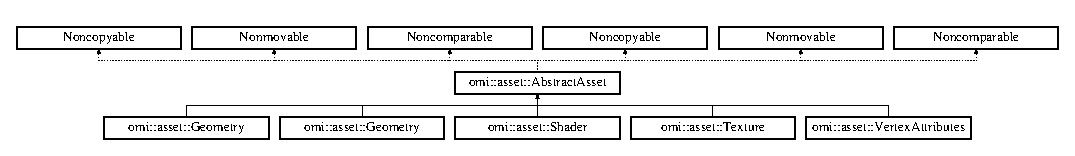
\includegraphics[height=1.647059cm]{classomi_1_1asset_1_1_abstract_asset}
\end{center}
\end{figure}
\subsection*{Classes}
\begin{DoxyCompactItemize}
\item 
class \hyperlink{classomi_1_1asset_1_1_abstract_asset_1_1_abstract_resource}{Abstract\+Resource}
\end{DoxyCompactItemize}


The documentation for this class was generated from the following file\+:\begin{DoxyCompactItemize}
\item 
/home/david/\+Dropbox/\+Development/\+Omicron/\+Omicron/src/cpp/omicron/api/asset/types/\hyperlink{_abstract_asset_8hpp}{Abstract\+Asset.\+hpp}\end{DoxyCompactItemize}

\hypertarget{classomi_1_1xform_1_1_abstract_constraint}{}\section{omi\+:\+:xform\+:\+:Abstract\+Constraint Class Reference}
\label{classomi_1_1xform_1_1_abstract_constraint}\index{omi\+::xform\+::\+Abstract\+Constraint@{omi\+::xform\+::\+Abstract\+Constraint}}


T\+O\+DO\+:  




{\ttfamily \#include $<$Abstract\+Constraint.\+hpp$>$}

Inheritance diagram for omi\+:\+:xform\+:\+:Abstract\+Constraint\+:\begin{figure}[H]
\begin{center}
\leavevmode
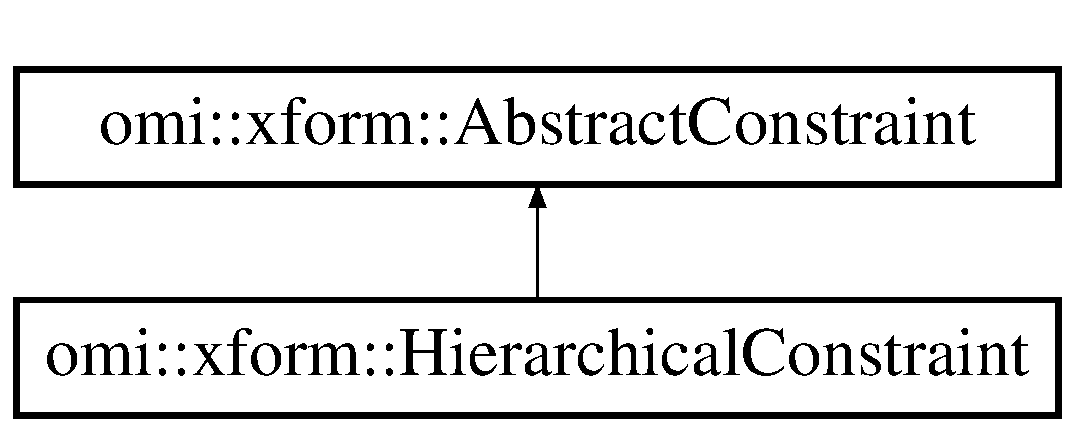
\includegraphics[height=2.000000cm]{classomi_1_1xform_1_1_abstract_constraint}
\end{center}
\end{figure}


\subsection{Detailed Description}
T\+O\+DO\+: 

The documentation for this class was generated from the following file\+:\begin{DoxyCompactItemize}
\item 
/home/david/\+Dropbox/\+Development/\+Omicron/\+Omicron/src/cpp/omicron/api/xform/\hyperlink{_abstract_constraint_8hpp}{Abstract\+Constraint.\+hpp}\end{DoxyCompactItemize}

\hypertarget{classomi_1_1asset_1_1_abstract_resource}{}\section{omi\+:\+:asset\+:\+:Abstract\+Resource Class Reference}
\label{classomi_1_1asset_1_1_abstract_resource}\index{omi\+::asset\+::\+Abstract\+Resource@{omi\+::asset\+::\+Abstract\+Resource}}
Inheritance diagram for omi\+:\+:asset\+:\+:Abstract\+Resource\+:\begin{figure}[H]
\begin{center}
\leavevmode
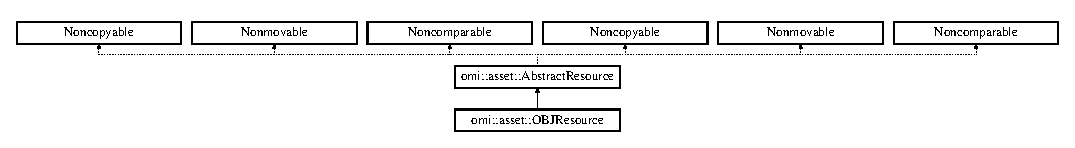
\includegraphics[height=1.546961cm]{classomi_1_1asset_1_1_abstract_resource}
\end{center}
\end{figure}
\subsection*{Public Member Functions}
\begin{DoxyCompactItemize}
\item 
virtual O\+M\+I\+\_\+\+A\+P\+I\+\_\+\+G\+L\+O\+B\+AL void {\bfseries load} (arc\+::io\+::sys\+::\+File\+Reader $\ast$reader)=0\hypertarget{classomi_1_1asset_1_1_abstract_resource_a02cc704cd296f2488fe365482d9831c4}{}\label{classomi_1_1asset_1_1_abstract_resource_a02cc704cd296f2488fe365482d9831c4}

\item 
virtual O\+M\+I\+\_\+\+A\+P\+I\+\_\+\+G\+L\+O\+B\+AL void {\bfseries release} ()=0\hypertarget{classomi_1_1asset_1_1_abstract_resource_ace554a5703b61f7ebf3ba67273093671}{}\label{classomi_1_1asset_1_1_abstract_resource_ace554a5703b61f7ebf3ba67273093671}

\item 
virtual O\+M\+I\+\_\+\+A\+P\+I\+\_\+\+G\+L\+O\+B\+AL void {\bfseries load} (arc\+::io\+::sys\+::\+File\+Reader $\ast$reader)=0\hypertarget{classomi_1_1asset_1_1_abstract_resource_a02cc704cd296f2488fe365482d9831c4}{}\label{classomi_1_1asset_1_1_abstract_resource_a02cc704cd296f2488fe365482d9831c4}

\item 
virtual O\+M\+I\+\_\+\+A\+P\+I\+\_\+\+G\+L\+O\+B\+AL void {\bfseries release} ()=0\hypertarget{classomi_1_1asset_1_1_abstract_resource_ace554a5703b61f7ebf3ba67273093671}{}\label{classomi_1_1asset_1_1_abstract_resource_ace554a5703b61f7ebf3ba67273093671}

\end{DoxyCompactItemize}


The documentation for this class was generated from the following files\+:\begin{DoxyCompactItemize}
\item 
/home/david/\+Dropbox/\+Development/\+Omicron/\+Omicron/src/cpp/omicron/api/asset/resource/\hyperlink{_abstract_resource_8hpp}{Abstract\+Resource.\+hpp}\item 
/home/david/\+Dropbox/\+Development/\+Omicron/\+Omicron/src/cpp/omicron/api/asset/\hyperlink{_resource_8hpp}{Resource.\+hpp}\end{DoxyCompactItemize}

\hypertarget{classomi_1_1asset_1_1_abstract_asset_1_1_abstract_resource}{}\section{omi\+:\+:asset\+:\+:Abstract\+Asset\+:\+:Abstract\+Resource Class Reference}
\label{classomi_1_1asset_1_1_abstract_asset_1_1_abstract_resource}\index{omi\+::asset\+::\+Abstract\+Asset\+::\+Abstract\+Resource@{omi\+::asset\+::\+Abstract\+Asset\+::\+Abstract\+Resource}}
Inheritance diagram for omi\+:\+:asset\+:\+:Abstract\+Asset\+:\+:Abstract\+Resource\+:\begin{figure}[H]
\begin{center}
\leavevmode
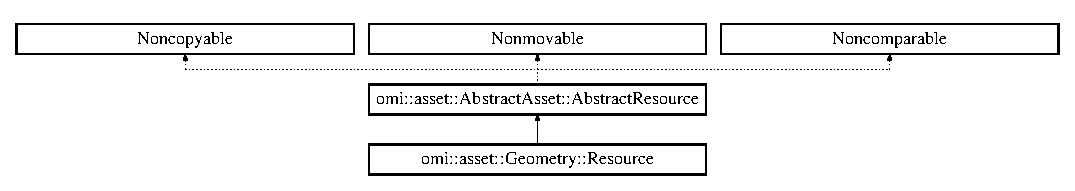
\includegraphics[height=2.113208cm]{classomi_1_1asset_1_1_abstract_asset_1_1_abstract_resource}
\end{center}
\end{figure}


The documentation for this class was generated from the following file\+:\begin{DoxyCompactItemize}
\item 
/home/david/\+Dropbox/\+Development/\+Omicron/\+Omicron/src/cpp/omicron/api/asset/types/\hyperlink{_abstract_asset_8hpp}{Abstract\+Asset.\+hpp}\end{DoxyCompactItemize}

\hypertarget{classomi_1_1runtime_1_1ss_1_1_abstract_subsystem}{}\section{omi\+:\+:runtime\+:\+:ss\+:\+:Abstract\+Subsystem Class Reference}
\label{classomi_1_1runtime_1_1ss_1_1_abstract_subsystem}\index{omi\+::runtime\+::ss\+::\+Abstract\+Subsystem@{omi\+::runtime\+::ss\+::\+Abstract\+Subsystem}}


Abstract base class that defines an object which manages the components used to access an Omicron subsystem.  




{\ttfamily \#include $<$Abstract\+Subsystem.\+hpp$>$}

Inheritance diagram for omi\+:\+:runtime\+:\+:ss\+:\+:Abstract\+Subsystem\+:\begin{figure}[H]
\begin{center}
\leavevmode
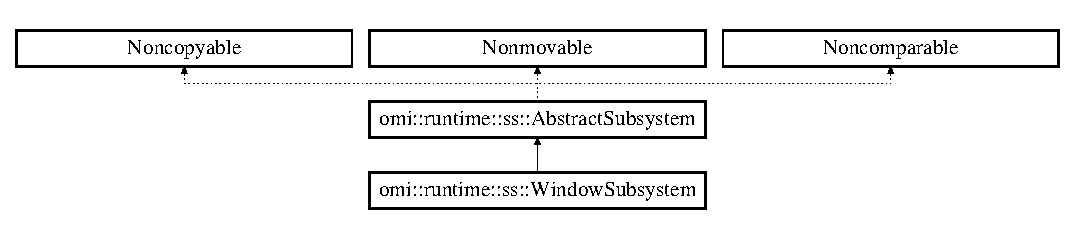
\includegraphics[height=2.580645cm]{classomi_1_1runtime_1_1ss_1_1_abstract_subsystem}
\end{center}
\end{figure}
\subsection*{Public Member Functions}
\begin{DoxyCompactItemize}
\item 
virtual void \hyperlink{classomi_1_1runtime_1_1ss_1_1_abstract_subsystem_a1d6cd9226416502ea0be8d1920a83cca}{bind} (arc\+::io\+::dl\+::\+Handle library)=0\hypertarget{classomi_1_1runtime_1_1ss_1_1_abstract_subsystem_a1d6cd9226416502ea0be8d1920a83cca}{}\label{classomi_1_1runtime_1_1ss_1_1_abstract_subsystem_a1d6cd9226416502ea0be8d1920a83cca}

\begin{DoxyCompactList}\small\item\em Loads the subsystem from the given dynamic library and binds it into Omicron. \end{DoxyCompactList}\item 
virtual void \hyperlink{classomi_1_1runtime_1_1ss_1_1_abstract_subsystem_ac8b1ad01306849a225c5d361abccf1cc}{startup} ()=0\hypertarget{classomi_1_1runtime_1_1ss_1_1_abstract_subsystem_ac8b1ad01306849a225c5d361abccf1cc}{}\label{classomi_1_1runtime_1_1ss_1_1_abstract_subsystem_ac8b1ad01306849a225c5d361abccf1cc}

\begin{DoxyCompactList}\small\item\em Starts up this subsystem. \end{DoxyCompactList}\item 
virtual void \hyperlink{classomi_1_1runtime_1_1ss_1_1_abstract_subsystem_ad5bf243e9a1b0ae94aaf3e6a998bdbf9}{release} ()=0
\begin{DoxyCompactList}\small\item\em Unbinds the subsystem from Omicron and shuts it down. \end{DoxyCompactList}\end{DoxyCompactItemize}


\subsection{Detailed Description}
Abstract base class that defines an object which manages the components used to access an Omicron subsystem. 

\subsection{Member Function Documentation}
\index{omi\+::runtime\+::ss\+::\+Abstract\+Subsystem@{omi\+::runtime\+::ss\+::\+Abstract\+Subsystem}!release@{release}}
\index{release@{release}!omi\+::runtime\+::ss\+::\+Abstract\+Subsystem@{omi\+::runtime\+::ss\+::\+Abstract\+Subsystem}}
\subsubsection[{\texorpdfstring{release()=0}{release()=0}}]{\setlength{\rightskip}{0pt plus 5cm}virtual void omi\+::runtime\+::ss\+::\+Abstract\+Subsystem\+::release (
\begin{DoxyParamCaption}
{}
\end{DoxyParamCaption}
)\hspace{0.3cm}{\ttfamily [pure virtual]}}\hypertarget{classomi_1_1runtime_1_1ss_1_1_abstract_subsystem_ad5bf243e9a1b0ae94aaf3e6a998bdbf9}{}\label{classomi_1_1runtime_1_1ss_1_1_abstract_subsystem_ad5bf243e9a1b0ae94aaf3e6a998bdbf9}


Unbinds the subsystem from Omicron and shuts it down. 

\begin{DoxyWarning}{Warning}
This should close the dynamic library, this is done by the \hyperlink{classomi_1_1runtime_1_1ss_1_1_subsystem_manager}{Subsystem\+Manager}. 
\end{DoxyWarning}


Implemented in \hyperlink{classomi_1_1runtime_1_1ss_1_1_window_subsystem_a86b3dbc5b0a67e77de1ca0cfe5cecbd8}{omi\+::runtime\+::ss\+::\+Window\+Subsystem}.



The documentation for this class was generated from the following file\+:\begin{DoxyCompactItemize}
\item 
/home/david/\+Dropbox/\+Development/\+Omicron/\+Omicron/src/cpp/omicron/runtime/subsystem/\hyperlink{_abstract_subsystem_8hpp}{Abstract\+Subsystem.\+hpp}\end{DoxyCompactItemize}

\hypertarget{classomi_1_1xform_1_1_abstract_transform}{}\section{omi\+:\+:xform\+:\+:Abstract\+Transform Class Reference}
\label{classomi_1_1xform_1_1_abstract_transform}\index{omi\+::xform\+::\+Abstract\+Transform@{omi\+::xform\+::\+Abstract\+Transform}}


T\+O\+DO\+:  




{\ttfamily \#include $<$Abstract\+Transform.\+hpp$>$}

Inheritance diagram for omi\+:\+:xform\+:\+:Abstract\+Transform\+:\begin{figure}[H]
\begin{center}
\leavevmode
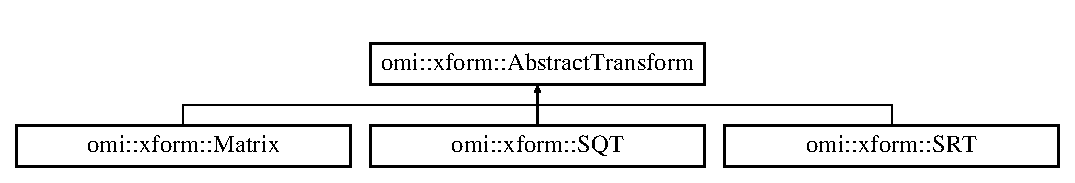
\includegraphics[height=2.000000cm]{classomi_1_1xform_1_1_abstract_transform}
\end{center}
\end{figure}


\subsection{Detailed Description}
T\+O\+DO\+: 

The documentation for this class was generated from the following file\+:\begin{DoxyCompactItemize}
\item 
/home/david/\+Dropbox/\+Development/\+Omicron/\+Omicron/src/cpp/omicron/api/xform/\hyperlink{_abstract_transform_8hpp}{Abstract\+Transform.\+hpp}\end{DoxyCompactItemize}

\hypertarget{class_a_l_subsystem}{}\section{A\+L\+Subsystem Class Reference}
\label{class_a_l_subsystem}\index{A\+L\+Subsystem@{A\+L\+Subsystem}}


T\+O\+DO.  




{\ttfamily \#include $<$A\+L\+Subsystem.\+hpp$>$}

Inheritance diagram for A\+L\+Subsystem\+:\begin{figure}[H]
\begin{center}
\leavevmode
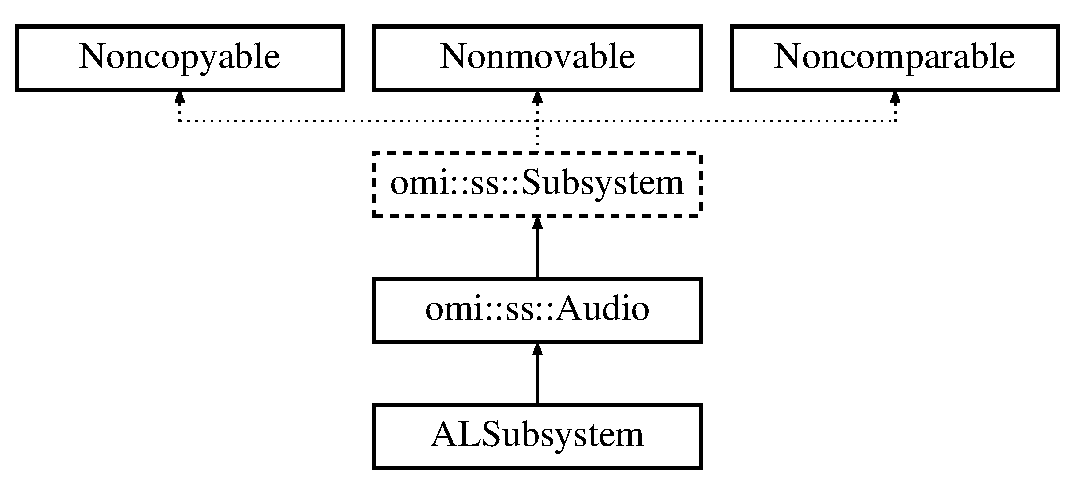
\includegraphics[height=4.000000cm]{class_a_l_subsystem}
\end{center}
\end{figure}
\subsection*{Public Member Functions}
\begin{DoxyCompactItemize}
\item 
virtual void \hyperlink{class_a_l_subsystem_a46de88998ac77d7d64532471d30028b3}{startup} ()
\begin{DoxyCompactList}\small\item\em Startups up this subsystem. \end{DoxyCompactList}\end{DoxyCompactItemize}
\subsection*{Additional Inherited Members}


\subsection{Detailed Description}
T\+O\+DO. 

\subsection{Member Function Documentation}
\index{A\+L\+Subsystem@{A\+L\+Subsystem}!startup@{startup}}
\index{startup@{startup}!A\+L\+Subsystem@{A\+L\+Subsystem}}
\subsubsection[{\texorpdfstring{startup()}{startup()}}]{\setlength{\rightskip}{0pt plus 5cm}virtual void A\+L\+Subsystem\+::startup (
\begin{DoxyParamCaption}
{}
\end{DoxyParamCaption}
)\hspace{0.3cm}{\ttfamily [virtual]}}\hypertarget{class_a_l_subsystem_a46de88998ac77d7d64532471d30028b3}{}\label{class_a_l_subsystem_a46de88998ac77d7d64532471d30028b3}


Startups up this subsystem. 

\begin{DoxyWarning}{Warning}
This function should not be called manually.
\end{DoxyWarning}
Other than the constructor, this will be the first call made to this object, and will only be called once. 

Reimplemented from \hyperlink{classomi_1_1ss_1_1_subsystem_a4b0ea0b6a120c551d73151f0e0432197}{omi\+::ss\+::\+Subsystem}.



The documentation for this class was generated from the following file\+:\begin{DoxyCompactItemize}
\item 
/home/david/\+Dropbox/\+Development/\+Omicron/\+Omicron/src/cpp/builtin\+\_\+subsystems/omi\+\_\+al/\hyperlink{_a_l_subsystem_8hpp}{A\+L\+Subsystem.\+hpp}\end{DoxyCompactItemize}

\hypertarget{classomi_1_1asset_1_1_asset_library}{}\section{omi\+:\+:asset\+:\+:Asset\+Library Class Reference}
\label{classomi_1_1asset_1_1_asset_library}\index{omi\+::asset\+::\+Asset\+Library@{omi\+::asset\+::\+Asset\+Library}}


Singleton object which is used to load, store, provide access to, and release game resources.  




{\ttfamily \#include $<$Asset\+Library.\+hpp$>$}

Inheritance diagram for omi\+:\+:asset\+:\+:Asset\+Library\+:\begin{figure}[H]
\begin{center}
\leavevmode
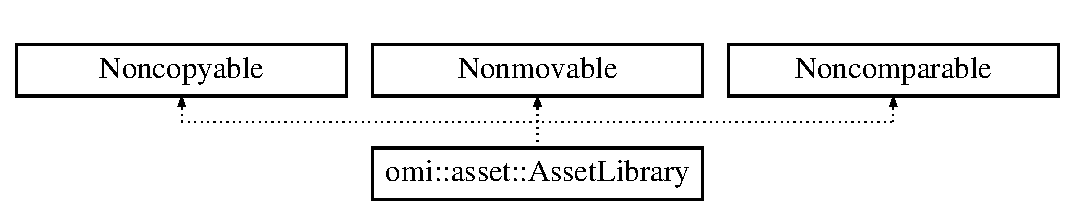
\includegraphics[height=2.000000cm]{classomi_1_1asset_1_1_asset_library}
\end{center}
\end{figure}
\subsection*{Static Public Member Functions}
\begin{DoxyCompactItemize}
\item 
static O\+M\+I\+\_\+\+A\+P\+I\+\_\+\+G\+L\+O\+B\+AL \hyperlink{classomi_1_1asset_1_1_asset_library}{Asset\+Library} $\ast$ \hyperlink{classomi_1_1asset_1_1_asset_library_a919ee8b0e034d68df7c333db4b274093}{instance} ()\hypertarget{classomi_1_1asset_1_1_asset_library_a919ee8b0e034d68df7c333db4b274093}{}\label{classomi_1_1asset_1_1_asset_library_a919ee8b0e034d68df7c333db4b274093}

\begin{DoxyCompactList}\small\item\em Returns the singleton instance of the \hyperlink{classomi_1_1asset_1_1_asset_library}{Asset\+Library}. \end{DoxyCompactList}\end{DoxyCompactItemize}


\subsection{Detailed Description}
Singleton object which is used to load, store, provide access to, and release game resources. 

\begin{DoxyRefDesc}{Todo}
\item[\hyperlink{todo__todo000001}{Todo}]\end{DoxyRefDesc}


The documentation for this class was generated from the following file\+:\begin{DoxyCompactItemize}
\item 
/home/david/\+Dropbox/\+Development/\+Omicron/\+Omicron/src/cpp/omicron/api/asset/\hyperlink{_asset_library_8hpp}{Asset\+Library.\+hpp}\end{DoxyCompactItemize}

\hypertarget{classomi_1_1_attribute}{}\section{omi\+:\+:Attribute Class Reference}
\label{classomi_1_1_attribute}\index{omi\+::\+Attribute@{omi\+::\+Attribute}}


The is the base class for all Omicron Attributes.  




{\ttfamily \#include $<$Attribute.\+hpp$>$}

Inheritance diagram for omi\+:\+:Attribute\+:\begin{figure}[H]
\begin{center}
\leavevmode
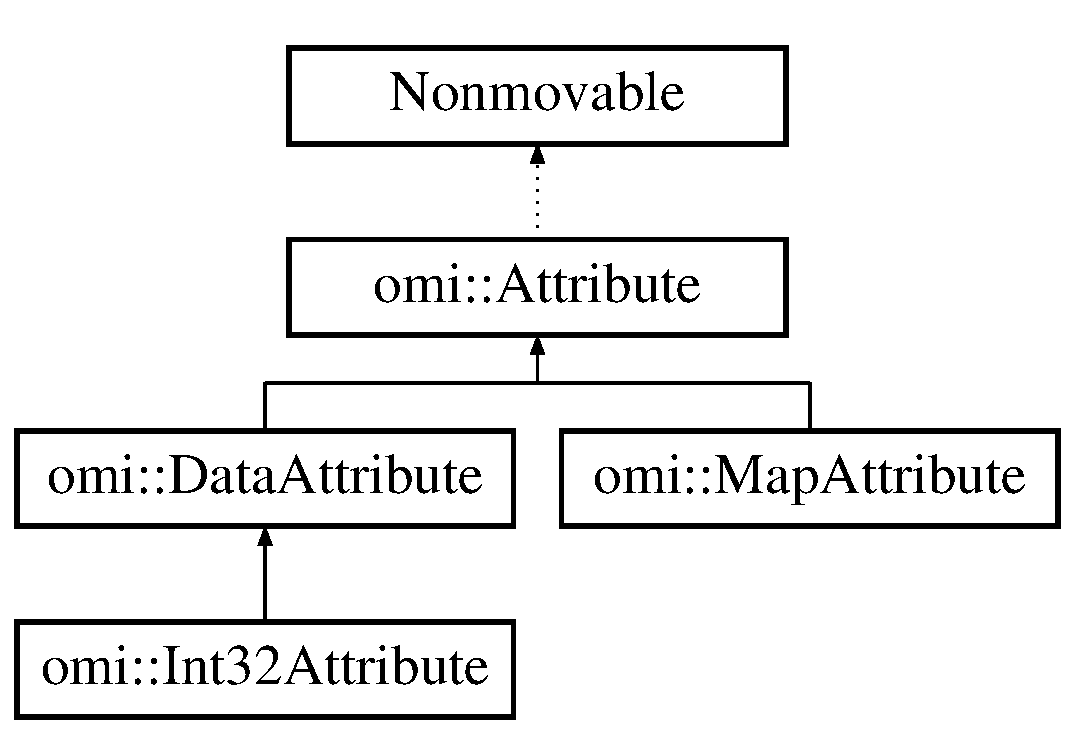
\includegraphics[height=4.000000cm]{classomi_1_1_attribute}
\end{center}
\end{figure}
\subsection*{Classes}
\begin{DoxyCompactItemize}
\item 
class \hyperlink{classomi_1_1_attribute_1_1_storage}{Storage}
\begin{DoxyCompactList}\small\item\em The internal storage class defines how the contents of the attribute will be stored. \end{DoxyCompactList}\end{DoxyCompactItemize}
\subsection*{Public Types}
\begin{DoxyCompactItemize}
\item 
typedef arc\+::int32 \hyperlink{classomi_1_1_attribute_aae4992bc8d2b12679548909bc813eecf}{Type}\hypertarget{classomi_1_1_attribute_aae4992bc8d2b12679548909bc813eecf}{}\label{classomi_1_1_attribute_aae4992bc8d2b12679548909bc813eecf}

\begin{DoxyCompactList}\small\item\em Integral type which defines the type identifier of an attribute. \end{DoxyCompactList}\end{DoxyCompactItemize}
\subsection*{Public Member Functions}
\begin{DoxyCompactItemize}
\item 
O\+M\+I\+\_\+\+A\+P\+I\+\_\+\+G\+L\+O\+B\+AL \hyperlink{classomi_1_1_attribute_a8dedd3d7b6659ce14e32712fcc729667}{Attribute} ()
\begin{DoxyCompactList}\small\item\em Constructs a new null attribute. \end{DoxyCompactList}\item 
O\+M\+I\+\_\+\+A\+P\+I\+\_\+\+G\+L\+O\+B\+AL \hyperlink{classomi_1_1_attribute_a53e38e8d8f7afd2dd26e52cc78fd7c79}{Attribute} (const \hyperlink{classomi_1_1_attribute}{Attribute} \&other)\hypertarget{classomi_1_1_attribute_a53e38e8d8f7afd2dd26e52cc78fd7c79}{}\label{classomi_1_1_attribute_a53e38e8d8f7afd2dd26e52cc78fd7c79}

\begin{DoxyCompactList}\small\item\em Constructs a new reference count of the given attribute. \end{DoxyCompactList}\item 
O\+M\+I\+\_\+\+A\+P\+I\+\_\+\+G\+L\+O\+B\+AL \hyperlink{classomi_1_1_attribute}{Attribute} \& \hyperlink{classomi_1_1_attribute_a01574090a4cd2f6bace4510dd54d3511}{operator=} (const \hyperlink{classomi_1_1_attribute}{Attribute} \&other)\hypertarget{classomi_1_1_attribute_a01574090a4cd2f6bace4510dd54d3511}{}\label{classomi_1_1_attribute_a01574090a4cd2f6bace4510dd54d3511}

\begin{DoxyCompactList}\small\item\em Assignment operator. \end{DoxyCompactList}\item 
O\+M\+I\+\_\+\+A\+P\+I\+\_\+\+G\+L\+O\+B\+AL bool \hyperlink{classomi_1_1_attribute_af2c5d727582a0df0843d87e17b938e65}{operator==} (const \hyperlink{classomi_1_1_attribute}{Attribute} \&other)\hypertarget{classomi_1_1_attribute_af2c5d727582a0df0843d87e17b938e65}{}\label{classomi_1_1_attribute_af2c5d727582a0df0843d87e17b938e65}

\begin{DoxyCompactList}\small\item\em Equality operator. \end{DoxyCompactList}\item 
O\+M\+I\+\_\+\+A\+P\+I\+\_\+\+G\+L\+O\+B\+AL bool \hyperlink{classomi_1_1_attribute_a57b8235bb86ce63c2ba661e32dea232d}{operator!=} (const \hyperlink{classomi_1_1_attribute}{Attribute} \&other)\hypertarget{classomi_1_1_attribute_a57b8235bb86ce63c2ba661e32dea232d}{}\label{classomi_1_1_attribute_a57b8235bb86ce63c2ba661e32dea232d}

\begin{DoxyCompactList}\small\item\em Inequality operator. \end{DoxyCompactList}\item 
O\+M\+I\+\_\+\+A\+P\+I\+\_\+\+G\+L\+O\+B\+AL \hyperlink{classomi_1_1_attribute_aae4992bc8d2b12679548909bc813eecf}{Type} \hyperlink{classomi_1_1_attribute_a30e2d8416ee8f9f0f972ddbd2f6c135c}{get\+\_\+type} () const 
\begin{DoxyCompactList}\small\item\em Returns the type identifier of this attribute. \end{DoxyCompactList}\item 
O\+M\+I\+\_\+\+A\+P\+I\+\_\+\+G\+L\+O\+B\+AL bool \hyperlink{classomi_1_1_attribute_aa4b45d4043cffdd1c729c1d89a484324}{is\+\_\+valid} () const 
\begin{DoxyCompactList}\small\item\em Returns whether this attribute is valid. \end{DoxyCompactList}\item 
O\+M\+I\+\_\+\+A\+P\+I\+\_\+\+G\+L\+O\+B\+AL bool \hyperlink{classomi_1_1_attribute_a33a211557a8c81e83ba3ada08f7198f1}{is\+\_\+immutable} () const 
\begin{DoxyCompactList}\small\item\em Returns whether this attribute is immutable or not. \end{DoxyCompactList}\item 
O\+M\+I\+\_\+\+A\+P\+I\+\_\+\+G\+L\+O\+B\+AL void \hyperlink{classomi_1_1_attribute_aa349cb49ea5438fb35d7929e755ea04f}{assign} (const \hyperlink{classomi_1_1_attribute}{Attribute} \&other)
\begin{DoxyCompactList}\small\item\em Attempts to a new reference count of the given \hyperlink{classomi_1_1_attribute}{Attribute}. \end{DoxyCompactList}\item 
O\+M\+I\+\_\+\+A\+P\+I\+\_\+\+G\+L\+O\+B\+AL \hyperlink{classomi_1_1_attribute}{Attribute} {\bfseries as\+\_\+immutable} () const \hypertarget{classomi_1_1_attribute_a37e99eea4065c73b3b0090397aef4bcc}{}\label{classomi_1_1_attribute_a37e99eea4065c73b3b0090397aef4bcc}

\item 
O\+M\+I\+\_\+\+A\+P\+I\+\_\+\+G\+L\+O\+B\+AL \hyperlink{classomi_1_1_attribute}{Attribute} {\bfseries as\+\_\+mutable} () const \hypertarget{classomi_1_1_attribute_a55eaada612dc1c74f80e4373dbc3635c}{}\label{classomi_1_1_attribute_a55eaada612dc1c74f80e4373dbc3635c}

\item 
O\+M\+I\+\_\+\+A\+P\+I\+\_\+\+G\+L\+O\+B\+AL void \hyperlink{classomi_1_1_attribute_a643b44b90d0c4e057624f5d8949c625a}{string\+\_\+repr} (arc\+::str\+::\+U\+T\+F8\+String \&s, std\+::size\+\_\+t indentation=0) const 
\begin{DoxyCompactList}\small\item\em Appends the string representation of this attribute (using the given indentation amount) to the provided string. \end{DoxyCompactList}\end{DoxyCompactItemize}
\subsection*{Static Public Attributes}
\begin{DoxyCompactItemize}
\item 
static O\+M\+I\+\_\+\+A\+P\+I\+\_\+\+G\+L\+O\+B\+AL \hyperlink{classomi_1_1_attribute_aae4992bc8d2b12679548909bc813eecf}{Type} \hyperlink{classomi_1_1_attribute_ad919ae1483da537cec6e46b7debfaa89}{k\+Type\+Null}\hypertarget{classomi_1_1_attribute_ad919ae1483da537cec6e46b7debfaa89}{}\label{classomi_1_1_attribute_ad919ae1483da537cec6e46b7debfaa89}

\begin{DoxyCompactList}\small\item\em The type identifier for null attributes. \end{DoxyCompactList}\end{DoxyCompactItemize}
\subsection*{Protected Member Functions}
\begin{DoxyCompactItemize}
\item 
O\+M\+I\+\_\+\+A\+P\+I\+\_\+\+G\+L\+O\+B\+AL \hyperlink{classomi_1_1_attribute_a15189f5bfe2cb81dbdafeb29f21ea8f0}{Attribute} (Definition $\ast$def)\hypertarget{classomi_1_1_attribute_a15189f5bfe2cb81dbdafeb29f21ea8f0}{}\label{classomi_1_1_attribute_a15189f5bfe2cb81dbdafeb29f21ea8f0}

\begin{DoxyCompactList}\small\item\em Super constructor which assigns the internal definition to the given object {\bfseries without} reference counting it. \end{DoxyCompactList}\item 
O\+M\+I\+\_\+\+A\+P\+I\+\_\+\+G\+L\+O\+B\+AL {\bfseries Attribute} (\hyperlink{classomi_1_1_attribute_aae4992bc8d2b12679548909bc813eecf}{Type} type, bool immutable, \hyperlink{classomi_1_1_attribute_1_1_storage}{Storage} $\ast$storage)\hypertarget{classomi_1_1_attribute_afd71075a24cf929b354cf9e8f89573d1}{}\label{classomi_1_1_attribute_afd71075a24cf929b354cf9e8f89573d1}

\item 
virtual O\+M\+I\+\_\+\+A\+P\+I\+\_\+\+G\+L\+O\+B\+AL bool \hyperlink{classomi_1_1_attribute_a351ac19ef02851d238f44bd2a101942c}{check\+\_\+type} (\hyperlink{classomi_1_1_attribute_aae4992bc8d2b12679548909bc813eecf}{Type} type) const \hypertarget{classomi_1_1_attribute_a351ac19ef02851d238f44bd2a101942c}{}\label{classomi_1_1_attribute_a351ac19ef02851d238f44bd2a101942c}

\begin{DoxyCompactList}\small\item\em Checks whether the given type is valid for this attribute. \end{DoxyCompactList}\item 
O\+M\+I\+\_\+\+A\+P\+I\+\_\+\+G\+L\+O\+B\+AL void \hyperlink{classomi_1_1_attribute_a91ec44ea94595d5bfef1b1300d1492bb}{increase\+\_\+ref} ()\hypertarget{classomi_1_1_attribute_a91ec44ea94595d5bfef1b1300d1492bb}{}\label{classomi_1_1_attribute_a91ec44ea94595d5bfef1b1300d1492bb}

\begin{DoxyCompactList}\small\item\em Increases the reference count this attribute\textquotesingle{}s internal definition. \end{DoxyCompactList}\item 
O\+M\+I\+\_\+\+A\+P\+I\+\_\+\+G\+L\+O\+B\+AL void \hyperlink{classomi_1_1_attribute_afe11b45c8cb9191181e48f273752243f}{decrease\+\_\+ref} ()\hypertarget{classomi_1_1_attribute_afe11b45c8cb9191181e48f273752243f}{}\label{classomi_1_1_attribute_afe11b45c8cb9191181e48f273752243f}

\begin{DoxyCompactList}\small\item\em Decreases the reference count of this attribute\textquotesingle{}s internal definition, if the reference count reaches 0, the definition is deleted. \end{DoxyCompactList}\item 
{\footnotesize template$<$typename T\+\_\+\+Storage\+Type $>$ }\\T\+\_\+\+Storage\+Type $\ast$ \hyperlink{classomi_1_1_attribute_aa3371ea331f0b313dce3d9b117775ff8}{get\+\_\+storage} () const \hypertarget{classomi_1_1_attribute_aa3371ea331f0b313dce3d9b117775ff8}{}\label{classomi_1_1_attribute_aa3371ea331f0b313dce3d9b117775ff8}

\begin{DoxyCompactList}\small\item\em Returns the storage object of this attribute\textquotesingle{}s definition casted as a pointer to the given type. \end{DoxyCompactList}\item 
O\+M\+I\+\_\+\+A\+P\+I\+\_\+\+G\+L\+O\+B\+AL void {\bfseries prepare\+\_\+modifcation} (bool soft=false)\hypertarget{classomi_1_1_attribute_a37bbc9dd7aa5b5eca9be1b9d83d2a268}{}\label{classomi_1_1_attribute_a37bbc9dd7aa5b5eca9be1b9d83d2a268}

\item 
O\+M\+I\+\_\+\+A\+P\+I\+\_\+\+G\+L\+O\+B\+AL void \hyperlink{classomi_1_1_attribute_a08ee8d47ce7b971daf3906555a8cd536}{check\+\_\+state} (const arc\+::str\+::\+U\+T\+F8\+String \&message) const \hypertarget{classomi_1_1_attribute_a08ee8d47ce7b971daf3906555a8cd536}{}\label{classomi_1_1_attribute_a08ee8d47ce7b971daf3906555a8cd536}

\begin{DoxyCompactList}\small\item\em Convenience function that checks whether this attribute is valid and if it is not throws an arc\+::ex\+::\+State\+Error with the given message. \end{DoxyCompactList}\end{DoxyCompactItemize}
\subsection*{Friends}
\begin{DoxyCompactItemize}
\item 
O\+M\+I\+\_\+\+A\+P\+I\+\_\+\+G\+L\+O\+B\+AL arc\+::str\+::\+U\+T\+F8\+String \& \hyperlink{classomi_1_1_attribute_aab6bf26917cd74f870e8db73210c6063}{operator$<$$<$} (arc\+::str\+::\+U\+T\+F8\+String \&, const \hyperlink{classomi_1_1_attribute}{Attribute} \&)\hypertarget{classomi_1_1_attribute_aab6bf26917cd74f870e8db73210c6063}{}\label{classomi_1_1_attribute_aab6bf26917cd74f870e8db73210c6063}

\begin{DoxyCompactList}\small\item\em Appends a string representation of the \hyperlink{classomi_1_1_attribute}{Attribute} to the given U\+T\+F8\+String. \end{DoxyCompactList}\end{DoxyCompactItemize}


\subsection{Detailed Description}
The is the base class for all Omicron Attributes. 

Attributes are data containers that can be passed around generically. Attributes can be efficiently \char`\"{}casted\char`\"{} as any other \hyperlink{classomi_1_1_attribute}{Attribute} type that they derive from and then \char`\"{}re-\/casted\char`\"{} back to their original type with no data loss. In-\/fact Attributes can be casted to any other attribute type but unless is a cast to a derived type of the original type or the original type the result will be an invalid null attribute. Casting attributes is efficient because no actual copying of data is performed -\/ attributes use a copy-\/on-\/write model which means data is purely referenced counted between attributes until it\textquotesingle{}s modified.

Attributes can be group into four main categories\+:
\begin{DoxyItemize}
\item Null\+Attribute\+: Attributes that are invalid or are constructed from the base attribute type \hyperlink{classomi_1_1_attribute}{omi\+::\+Attribute}, these attributes are are a null type but always valid.
\item \hyperlink{classomi_1_1_data_attribute}{Data\+Attribute}\+: The most common attribute type which contains zero or more values of specific type, e.\+g. Float\+Attribute, \hyperlink{classomi_1_1_int32_attribute}{Int32\+Attribute}, etc.
\item Array\+Attribute\+: An attribute that contains an ordered array of zero or or more attributes.
\item \hyperlink{classomi_1_1_map_attribute}{Map\+Attribute}\+: An attribute which contains key values pairs of names and attributes. Map\+Attributes can be used to encode hierarchies by nesting Map\+Attributes.
\end{DoxyItemize}

An \hyperlink{classomi_1_1_attribute}{Attribute} can be checked to see if it\textquotesingle{}s valid using the \hyperlink{classomi_1_1_attribute_aa4b45d4043cffdd1c729c1d89a484324}{is\+\_\+valid()} function.

For example\+:


\begin{DoxyCode}
\hyperlink{classomi_1_1_int32_attribute}{omi::Int32Attribute} a(12);
\hyperlink{classomi_1_1_attribute}{omi::Attribute} b(a);
\hyperlink{classomi_1_1_int32_attribute}{omi::Int32Attribute} c(b);
c.is\_valid();
\end{DoxyCode}


Would return {\ttfamily true} since the original \hyperlink{classomi_1_1_int32_attribute}{Int32\+Attribute} has been casted to a type it was derived from then and then casted back to its original type.

However\+:


\begin{DoxyCode}
\hyperlink{classomi_1_1_int32_attribute}{omi::Int32Attribute} a(12);
omi::FloatAttribute b(a);
b.is\_valid();
\end{DoxyCode}


Would return {\ttfamily false} since the original \hyperlink{classomi_1_1_int32_attribute}{Int32\+Attribute} has been casted to an orthogonal type. 

\subsection{Constructor \& Destructor Documentation}
\index{omi\+::\+Attribute@{omi\+::\+Attribute}!Attribute@{Attribute}}
\index{Attribute@{Attribute}!omi\+::\+Attribute@{omi\+::\+Attribute}}
\subsubsection[{\texorpdfstring{Attribute()}{Attribute()}}]{\setlength{\rightskip}{0pt plus 5cm}O\+M\+I\+\_\+\+A\+P\+I\+\_\+\+G\+L\+O\+B\+AL omi\+::\+Attribute\+::\+Attribute (
\begin{DoxyParamCaption}
{}
\end{DoxyParamCaption}
)}\hypertarget{classomi_1_1_attribute_a8dedd3d7b6659ce14e32712fcc729667}{}\label{classomi_1_1_attribute_a8dedd3d7b6659ce14e32712fcc729667}


Constructs a new null attribute. 

\begin{DoxyNote}{Note}
This attribute is immutable by definition. 
\end{DoxyNote}


\subsection{Member Function Documentation}
\index{omi\+::\+Attribute@{omi\+::\+Attribute}!get\+\_\+type@{get\+\_\+type}}
\index{get\+\_\+type@{get\+\_\+type}!omi\+::\+Attribute@{omi\+::\+Attribute}}
\subsubsection[{\texorpdfstring{get\+\_\+type() const }{get_type() const }}]{\setlength{\rightskip}{0pt plus 5cm}O\+M\+I\+\_\+\+A\+P\+I\+\_\+\+G\+L\+O\+B\+AL {\bf Type} omi\+::\+Attribute\+::get\+\_\+type (
\begin{DoxyParamCaption}
{}
\end{DoxyParamCaption}
) const}\hypertarget{classomi_1_1_attribute_a30e2d8416ee8f9f0f972ddbd2f6c135c}{}\label{classomi_1_1_attribute_a30e2d8416ee8f9f0f972ddbd2f6c135c}


Returns the type identifier of this attribute. 

Each attribute type has a unique type attribute, which means checking the type of a base class attribute can be to check what the original type of the attribute is. \index{omi\+::\+Attribute@{omi\+::\+Attribute}!is\+\_\+valid@{is\+\_\+valid}}
\index{is\+\_\+valid@{is\+\_\+valid}!omi\+::\+Attribute@{omi\+::\+Attribute}}
\subsubsection[{\texorpdfstring{is\+\_\+valid() const }{is_valid() const }}]{\setlength{\rightskip}{0pt plus 5cm}O\+M\+I\+\_\+\+A\+P\+I\+\_\+\+G\+L\+O\+B\+AL bool omi\+::\+Attribute\+::is\+\_\+valid (
\begin{DoxyParamCaption}
{}
\end{DoxyParamCaption}
) const}\hypertarget{classomi_1_1_attribute_aa4b45d4043cffdd1c729c1d89a484324}{}\label{classomi_1_1_attribute_aa4b45d4043cffdd1c729c1d89a484324}


Returns whether this attribute is valid. 

Base attributes are always valid, but derived types will be invalid if they were casted from an incompatible type.

Invalid attributes will always return their type as \hyperlink{classomi_1_1_attribute_ad919ae1483da537cec6e46b7debfaa89}{omi\+::\+Attribute\+::k\+Type\+Null}. \index{omi\+::\+Attribute@{omi\+::\+Attribute}!is\+\_\+immutable@{is\+\_\+immutable}}
\index{is\+\_\+immutable@{is\+\_\+immutable}!omi\+::\+Attribute@{omi\+::\+Attribute}}
\subsubsection[{\texorpdfstring{is\+\_\+immutable() const }{is_immutable() const }}]{\setlength{\rightskip}{0pt plus 5cm}O\+M\+I\+\_\+\+A\+P\+I\+\_\+\+G\+L\+O\+B\+AL bool omi\+::\+Attribute\+::is\+\_\+immutable (
\begin{DoxyParamCaption}
{}
\end{DoxyParamCaption}
) const}\hypertarget{classomi_1_1_attribute_a33a211557a8c81e83ba3ada08f7198f1}{}\label{classomi_1_1_attribute_a33a211557a8c81e83ba3ada08f7198f1}


Returns whether this attribute is immutable or not. 

Immutable attributes will never copy storage and mutable attributes will only copy storage when they\textquotesingle{}re modified. \index{omi\+::\+Attribute@{omi\+::\+Attribute}!assign@{assign}}
\index{assign@{assign}!omi\+::\+Attribute@{omi\+::\+Attribute}}
\subsubsection[{\texorpdfstring{assign(const Attribute \&other)}{assign(const Attribute &other)}}]{\setlength{\rightskip}{0pt plus 5cm}O\+M\+I\+\_\+\+A\+P\+I\+\_\+\+G\+L\+O\+B\+AL void omi\+::\+Attribute\+::assign (
\begin{DoxyParamCaption}
\item[{const {\bf Attribute} \&}]{other}
\end{DoxyParamCaption}
)}\hypertarget{classomi_1_1_attribute_aa349cb49ea5438fb35d7929e755ea04f}{}\label{classomi_1_1_attribute_aa349cb49ea5438fb35d7929e755ea04f}


Attempts to a new reference count of the given \hyperlink{classomi_1_1_attribute}{Attribute}. 

If the given attribute is not a valid attribute type to copy from this will construct an invalid attribute. \index{omi\+::\+Attribute@{omi\+::\+Attribute}!string\+\_\+repr@{string\+\_\+repr}}
\index{string\+\_\+repr@{string\+\_\+repr}!omi\+::\+Attribute@{omi\+::\+Attribute}}
\subsubsection[{\texorpdfstring{string\+\_\+repr(arc\+::str\+::\+U\+T\+F8\+String \&s, std\+::size\+\_\+t indentation=0) const }{string_repr(arc::str::UTF8String &s, std::size_t indentation=0) const }}]{\setlength{\rightskip}{0pt plus 5cm}O\+M\+I\+\_\+\+A\+P\+I\+\_\+\+G\+L\+O\+B\+AL void omi\+::\+Attribute\+::string\+\_\+repr (
\begin{DoxyParamCaption}
\item[{arc\+::str\+::\+U\+T\+F8\+String \&}]{s, }
\item[{std\+::size\+\_\+t}]{indentation = {\ttfamily 0}}
\end{DoxyParamCaption}
) const}\hypertarget{classomi_1_1_attribute_a643b44b90d0c4e057624f5d8949c625a}{}\label{classomi_1_1_attribute_a643b44b90d0c4e057624f5d8949c625a}


Appends the string representation of this attribute (using the given indentation amount) to the provided string. 


\begin{DoxyParams}{Parameters}
{\em s} & The string to append this string representation. \\
\hline
{\em indentation} & The amount of indentation (in spaces) this attribute should be indented by. \\
\hline
\end{DoxyParams}


The documentation for this class was generated from the following file\+:\begin{DoxyCompactItemize}
\item 
/home/david/\+Dropbox/\+Development/\+Omicron/\+Omicron/src/cpp/omicron/api/common/attribute/\hyperlink{_attribute_8hpp}{Attribute.\+hpp}\end{DoxyCompactItemize}

\hypertarget{classomi_1_1ss_1_1_audio}{}\section{omi\+:\+:ss\+:\+:Audio Class Reference}
\label{classomi_1_1ss_1_1_audio}\index{omi\+::ss\+::\+Audio@{omi\+::ss\+::\+Audio}}


T\+O\+DO\+:  




{\ttfamily \#include $<$Audio.\+hpp$>$}

Inheritance diagram for omi\+:\+:ss\+:\+:Audio\+:\begin{figure}[H]
\begin{center}
\leavevmode
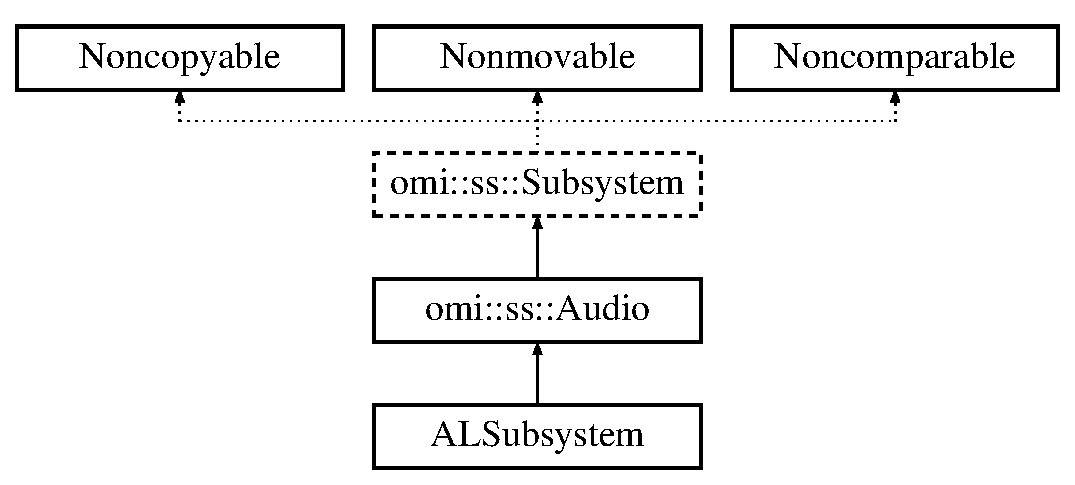
\includegraphics[height=4.000000cm]{classomi_1_1ss_1_1_audio}
\end{center}
\end{figure}
\subsection*{Public Member Functions}
\begin{DoxyCompactItemize}
\item 
\hyperlink{classomi_1_1ss_1_1_audio_a2f2223a266cde9309ef2a309a14f9520}{Audio} ()\hypertarget{classomi_1_1ss_1_1_audio_a2f2223a266cde9309ef2a309a14f9520}{}\label{classomi_1_1ss_1_1_audio_a2f2223a266cde9309ef2a309a14f9520}

\begin{DoxyCompactList}\small\item\em T\+O\+DO\+: \end{DoxyCompactList}\end{DoxyCompactItemize}
\subsection*{Additional Inherited Members}


\subsection{Detailed Description}
T\+O\+DO\+: 

The documentation for this class was generated from the following file\+:\begin{DoxyCompactItemize}
\item 
/home/david/\+Dropbox/\+Development/\+Omicron/\+Omicron/src/cpp/omicron/subsystem/\hyperlink{_audio_8hpp}{Audio.\+hpp}\end{DoxyCompactItemize}

\hypertarget{classomi_1_1window_1_1ss_1_1_bootstrap}{}\section{omi\+:\+:window\+:\+:ss\+:\+:Bootstrap Class Reference}
\label{classomi_1_1window_1_1ss_1_1_bootstrap}\index{omi\+::window\+::ss\+::\+Bootstrap@{omi\+::window\+::ss\+::\+Bootstrap}}


Object used to bootstrap a window subsystem and enters Omicron\textquotesingle{}s main loop.  




{\ttfamily \#include $<$Window\+Bootstrap.\+hpp$>$}

Inheritance diagram for omi\+:\+:window\+:\+:ss\+:\+:Bootstrap\+:\begin{figure}[H]
\begin{center}
\leavevmode
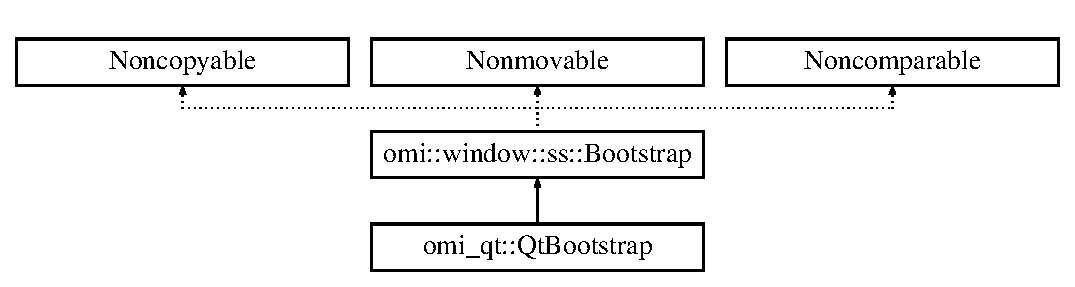
\includegraphics[height=3.000000cm]{classomi_1_1window_1_1ss_1_1_bootstrap}
\end{center}
\end{figure}
\subsection*{Public Member Functions}
\begin{DoxyCompactItemize}
\item 
virtual void \hyperlink{classomi_1_1window_1_1ss_1_1_bootstrap_a69b71f75e8be1496de09b3c5c647ded2}{startup} ()
\begin{DoxyCompactList}\small\item\em Starts up this Omicron window subsystem. \end{DoxyCompactList}\item 
virtual void \hyperlink{classomi_1_1window_1_1ss_1_1_bootstrap_a6e1b4cae0710d47c28de0cda82ef9378}{shutdown} ()
\begin{DoxyCompactList}\small\item\em Starts up this Omicron window subsystem. \end{DoxyCompactList}\item 
virtual void \hyperlink{classomi_1_1window_1_1ss_1_1_bootstrap_a412da1412bbf4e0c4eae29b04469a4e2}{start\+\_\+main\+\_\+loop} (\hyperlink{namespaceomi_1_1window_1_1ss_af42d2464a170bdfd876a35b9fde16137}{Engine\+Cycle\+Func} $\ast$engine\+\_\+cycle\+\_\+func)=0\hypertarget{classomi_1_1window_1_1ss_1_1_bootstrap_a412da1412bbf4e0c4eae29b04469a4e2}{}\label{classomi_1_1window_1_1ss_1_1_bootstrap_a412da1412bbf4e0c4eae29b04469a4e2}

\begin{DoxyCompactList}\small\item\em Starts the main loop of Omicron which will be managed by window subsystem and will call the given function every cycle of the main loop. \end{DoxyCompactList}\end{DoxyCompactItemize}
\subsection*{Protected Member Functions}
\begin{DoxyCompactItemize}
\item 
\hyperlink{classomi_1_1window_1_1ss_1_1_bootstrap_acf084e8d909c6a99a1afbbcb0a9199e7}{Bootstrap} ()\hypertarget{classomi_1_1window_1_1ss_1_1_bootstrap_acf084e8d909c6a99a1afbbcb0a9199e7}{}\label{classomi_1_1window_1_1ss_1_1_bootstrap_acf084e8d909c6a99a1afbbcb0a9199e7}

\begin{DoxyCompactList}\small\item\em Super constructor for window subsystem bootstrappers. \end{DoxyCompactList}\end{DoxyCompactItemize}


\subsection{Detailed Description}
Object used to bootstrap a window subsystem and enters Omicron\textquotesingle{}s main loop. 

\subsection{Member Function Documentation}
\index{omi\+::window\+::ss\+::\+Bootstrap@{omi\+::window\+::ss\+::\+Bootstrap}!startup@{startup}}
\index{startup@{startup}!omi\+::window\+::ss\+::\+Bootstrap@{omi\+::window\+::ss\+::\+Bootstrap}}
\subsubsection[{\texorpdfstring{startup()}{startup()}}]{\setlength{\rightskip}{0pt plus 5cm}virtual void omi\+::window\+::ss\+::\+Bootstrap\+::startup (
\begin{DoxyParamCaption}
{}
\end{DoxyParamCaption}
)\hspace{0.3cm}{\ttfamily [inline]}, {\ttfamily [virtual]}}\hypertarget{classomi_1_1window_1_1ss_1_1_bootstrap_a69b71f75e8be1496de09b3c5c647ded2}{}\label{classomi_1_1window_1_1ss_1_1_bootstrap_a69b71f75e8be1496de09b3c5c647ded2}


Starts up this Omicron window subsystem. 

Other than the \hyperlink{classomi_1_1window_1_1ss_1_1_bootstrap}{Bootstrap}\textquotesingle{}s constructor this will be the first call made to this object, and will only be made once. 

Reimplemented in \hyperlink{classomi__qt_1_1_qt_bootstrap_ae86dd5217529263238e51228c248e74f}{omi\+\_\+qt\+::\+Qt\+Bootstrap}.

\index{omi\+::window\+::ss\+::\+Bootstrap@{omi\+::window\+::ss\+::\+Bootstrap}!shutdown@{shutdown}}
\index{shutdown@{shutdown}!omi\+::window\+::ss\+::\+Bootstrap@{omi\+::window\+::ss\+::\+Bootstrap}}
\subsubsection[{\texorpdfstring{shutdown()}{shutdown()}}]{\setlength{\rightskip}{0pt plus 5cm}virtual void omi\+::window\+::ss\+::\+Bootstrap\+::shutdown (
\begin{DoxyParamCaption}
{}
\end{DoxyParamCaption}
)\hspace{0.3cm}{\ttfamily [inline]}, {\ttfamily [virtual]}}\hypertarget{classomi_1_1window_1_1ss_1_1_bootstrap_a6e1b4cae0710d47c28de0cda82ef9378}{}\label{classomi_1_1window_1_1ss_1_1_bootstrap_a6e1b4cae0710d47c28de0cda82ef9378}


Starts up this Omicron window subsystem. 

Other than the \hyperlink{classomi_1_1window_1_1ss_1_1_bootstrap}{Bootstrap}\textquotesingle{}s destructor this will be the last call made to this object, and will only be made once. 

Reimplemented in \hyperlink{classomi__qt_1_1_qt_bootstrap_a80d703cd4cb032ed900c1d77ea0056ab}{omi\+\_\+qt\+::\+Qt\+Bootstrap}.



The documentation for this class was generated from the following file\+:\begin{DoxyCompactItemize}
\item 
/home/david/\+Dropbox/\+Development/\+Omicron/\+Omicron/src/cpp/omicron/api/window/subsystem/\hyperlink{_window_bootstrap_8hpp}{Window\+Bootstrap.\+hpp}\end{DoxyCompactItemize}

\hypertarget{classomi_1_1render_1_1ss_1_1_bootstrap}{}\section{omi\+:\+:render\+:\+:ss\+:\+:Bootstrap Class Reference}
\label{classomi_1_1render_1_1ss_1_1_bootstrap}\index{omi\+::render\+::ss\+::\+Bootstrap@{omi\+::render\+::ss\+::\+Bootstrap}}


Object used to bootstrap a rendering subsystem.  




{\ttfamily \#include $<$Render\+Bootstrap.\+hpp$>$}

Inheritance diagram for omi\+:\+:render\+:\+:ss\+:\+:Bootstrap\+:\begin{figure}[H]
\begin{center}
\leavevmode
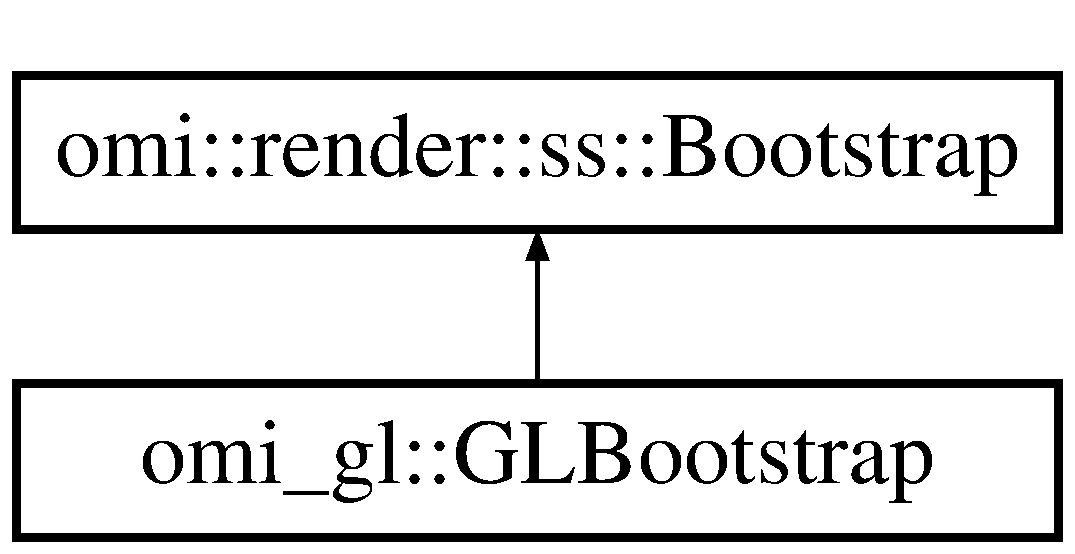
\includegraphics[height=2.000000cm]{classomi_1_1render_1_1ss_1_1_bootstrap}
\end{center}
\end{figure}
\subsection*{Public Member Functions}
\begin{DoxyCompactItemize}
\item 
virtual void \hyperlink{classomi_1_1render_1_1ss_1_1_bootstrap_a3b7e12774f56ce17baee150c5c85e1cb}{startup} ()
\begin{DoxyCompactList}\small\item\em Starts up this Omicron rendering subsystem. \end{DoxyCompactList}\item 
virtual void \hyperlink{classomi_1_1render_1_1ss_1_1_bootstrap_af4f13ba4968f7dac6141a7c558188aaf}{shutdown} ()
\begin{DoxyCompactList}\small\item\em Starts up this Omicron rendering subsystem. \end{DoxyCompactList}\end{DoxyCompactItemize}
\subsection*{Protected Member Functions}
\begin{DoxyCompactItemize}
\item 
\hyperlink{classomi_1_1render_1_1ss_1_1_bootstrap_a1ebc5b7615d6a3258a2fbeca135e8fae}{Bootstrap} ()\hypertarget{classomi_1_1render_1_1ss_1_1_bootstrap_a1ebc5b7615d6a3258a2fbeca135e8fae}{}\label{classomi_1_1render_1_1ss_1_1_bootstrap_a1ebc5b7615d6a3258a2fbeca135e8fae}

\begin{DoxyCompactList}\small\item\em Super constructor for rendering subsystem bootstrappers. \end{DoxyCompactList}\end{DoxyCompactItemize}


\subsection{Detailed Description}
Object used to bootstrap a rendering subsystem. 

\subsection{Member Function Documentation}
\index{omi\+::render\+::ss\+::\+Bootstrap@{omi\+::render\+::ss\+::\+Bootstrap}!startup@{startup}}
\index{startup@{startup}!omi\+::render\+::ss\+::\+Bootstrap@{omi\+::render\+::ss\+::\+Bootstrap}}
\subsubsection[{\texorpdfstring{startup()}{startup()}}]{\setlength{\rightskip}{0pt plus 5cm}virtual void omi\+::render\+::ss\+::\+Bootstrap\+::startup (
\begin{DoxyParamCaption}
{}
\end{DoxyParamCaption}
)\hspace{0.3cm}{\ttfamily [inline]}, {\ttfamily [virtual]}}\hypertarget{classomi_1_1render_1_1ss_1_1_bootstrap_a3b7e12774f56ce17baee150c5c85e1cb}{}\label{classomi_1_1render_1_1ss_1_1_bootstrap_a3b7e12774f56ce17baee150c5c85e1cb}


Starts up this Omicron rendering subsystem. 

Other than the \hyperlink{classomi_1_1render_1_1ss_1_1_bootstrap}{Bootstrap}\textquotesingle{}s constructor this will be the first call made to this object, and will only be made once. 

Reimplemented in \hyperlink{classomi__gl_1_1_g_l_bootstrap_a2cb4f9ea291138b1fb0943a6957f89c5}{omi\+\_\+gl\+::\+G\+L\+Bootstrap}.

\index{omi\+::render\+::ss\+::\+Bootstrap@{omi\+::render\+::ss\+::\+Bootstrap}!shutdown@{shutdown}}
\index{shutdown@{shutdown}!omi\+::render\+::ss\+::\+Bootstrap@{omi\+::render\+::ss\+::\+Bootstrap}}
\subsubsection[{\texorpdfstring{shutdown()}{shutdown()}}]{\setlength{\rightskip}{0pt plus 5cm}virtual void omi\+::render\+::ss\+::\+Bootstrap\+::shutdown (
\begin{DoxyParamCaption}
{}
\end{DoxyParamCaption}
)\hspace{0.3cm}{\ttfamily [inline]}, {\ttfamily [virtual]}}\hypertarget{classomi_1_1render_1_1ss_1_1_bootstrap_af4f13ba4968f7dac6141a7c558188aaf}{}\label{classomi_1_1render_1_1ss_1_1_bootstrap_af4f13ba4968f7dac6141a7c558188aaf}


Starts up this Omicron rendering subsystem. 

Other than the \hyperlink{classomi_1_1render_1_1ss_1_1_bootstrap}{Bootstrap}\textquotesingle{}s destructor this will be the last call made to this object, and will only be made once. 

Reimplemented in \hyperlink{classomi__gl_1_1_g_l_bootstrap_ae086f372b2f8e5b56087bb28c4310d14}{omi\+\_\+gl\+::\+G\+L\+Bootstrap}.



The documentation for this class was generated from the following file\+:\begin{DoxyCompactItemize}
\item 
/home/david/\+Dropbox/\+Development/\+Omicron/\+Omicron/src/cpp/omicron/api/render/subsystem/\hyperlink{_render_bootstrap_8hpp}{Render\+Bootstrap.\+hpp}\end{DoxyCompactItemize}

\hypertarget{class_bullet_subsystem}{}\section{Bullet\+Subsystem Class Reference}
\label{class_bullet_subsystem}\index{Bullet\+Subsystem@{Bullet\+Subsystem}}


T\+O\+DO.  




{\ttfamily \#include $<$Bullet\+Subsystem.\+hpp$>$}

Inheritance diagram for Bullet\+Subsystem\+:\begin{figure}[H]
\begin{center}
\leavevmode
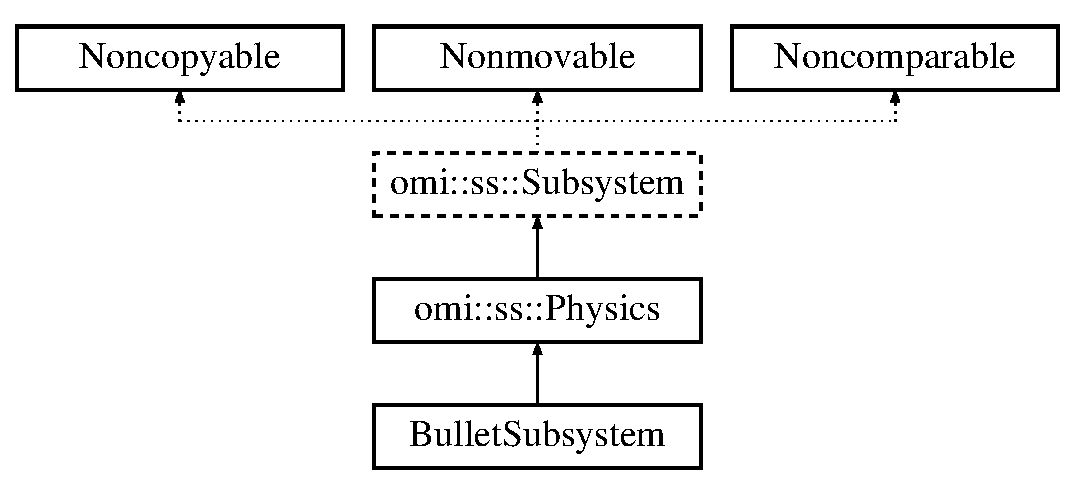
\includegraphics[height=4.000000cm]{class_bullet_subsystem}
\end{center}
\end{figure}
\subsection*{Public Member Functions}
\begin{DoxyCompactItemize}
\item 
virtual void \hyperlink{class_bullet_subsystem_a3221cf461749b3b7a4a9a9784f06b5b4}{startup} ()
\begin{DoxyCompactList}\small\item\em Startups up this subsystem. \end{DoxyCompactList}\end{DoxyCompactItemize}
\subsection*{Additional Inherited Members}


\subsection{Detailed Description}
T\+O\+DO. 

\subsection{Member Function Documentation}
\index{Bullet\+Subsystem@{Bullet\+Subsystem}!startup@{startup}}
\index{startup@{startup}!Bullet\+Subsystem@{Bullet\+Subsystem}}
\subsubsection[{\texorpdfstring{startup()}{startup()}}]{\setlength{\rightskip}{0pt plus 5cm}virtual void Bullet\+Subsystem\+::startup (
\begin{DoxyParamCaption}
{}
\end{DoxyParamCaption}
)\hspace{0.3cm}{\ttfamily [virtual]}}\hypertarget{class_bullet_subsystem_a3221cf461749b3b7a4a9a9784f06b5b4}{}\label{class_bullet_subsystem_a3221cf461749b3b7a4a9a9784f06b5b4}


Startups up this subsystem. 

\begin{DoxyWarning}{Warning}
This function should not be called manually.
\end{DoxyWarning}
Other than the constructor, this will be the first call made to this object, and will only be called once. 

Reimplemented from \hyperlink{classomi_1_1ss_1_1_subsystem_a4b0ea0b6a120c551d73151f0e0432197}{omi\+::ss\+::\+Subsystem}.



The documentation for this class was generated from the following file\+:\begin{DoxyCompactItemize}
\item 
/home/david/\+Dropbox/\+Development/\+Omicron/\+Omicron/src/cpp/builtin\+\_\+subsystems/omi\+\_\+bullet/\hyperlink{_bullet_subsystem_8hpp}{Bullet\+Subsystem.\+hpp}\end{DoxyCompactItemize}

\hypertarget{class_camera}{}\section{Camera Class Reference}
\label{class_camera}\index{Camera@{Camera}}
Inheritance diagram for Camera\+:\begin{figure}[H]
\begin{center}
\leavevmode
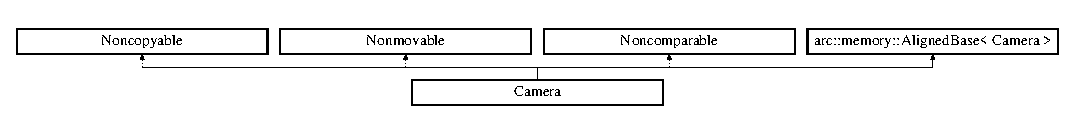
\includegraphics[height=1.196581cm]{class_camera}
\end{center}
\end{figure}
\subsection*{Public Member Functions}
\begin{DoxyCompactItemize}
\item 
{\bfseries Camera} (float focal\+\_\+length)\hypertarget{class_camera_ac04731f6e389bd64b66d6a73a3cab02c}{}\label{class_camera_ac04731f6e389bd64b66d6a73a3cab02c}

\item 
float {\bfseries get\+\_\+focal\+\_\+length} () const \hypertarget{class_camera_a3656ec90c9a6ec3d4686e825445780cb}{}\label{class_camera_a3656ec90c9a6ec3d4686e825445780cb}

\item 
const arc\+::gm\+::\+Simd\+Vector3f \& {\bfseries get\+\_\+focal\+\_\+point} () const \hypertarget{class_camera_ac578aecaf759fc92f85f8bd4c06cd860}{}\label{class_camera_ac578aecaf759fc92f85f8bd4c06cd860}

\item 
void {\bfseries set\+\_\+focal\+\_\+length} (float focal\+\_\+length)\hypertarget{class_camera_af040e8de4fcaff522ddeade8342eaf51}{}\label{class_camera_af040e8de4fcaff522ddeade8342eaf51}

\end{DoxyCompactItemize}


The documentation for this class was generated from the following file\+:\begin{DoxyCompactItemize}
\item 
/home/david/\+Dropbox/\+Development/\+Omicron/\+Omicron/src/cpp/builtin\+\_\+subsystems/pxtrace/\hyperlink{_camera_8hpp}{Camera.\+hpp}\end{DoxyCompactItemize}

\hypertarget{classomi_1_1_data_attribute}{}\section{omi\+:\+:Data\+Attribute Class Reference}
\label{classomi_1_1_data_attribute}\index{omi\+::\+Data\+Attribute@{omi\+::\+Data\+Attribute}}
Inheritance diagram for omi\+:\+:Data\+Attribute\+:\begin{figure}[H]
\begin{center}
\leavevmode
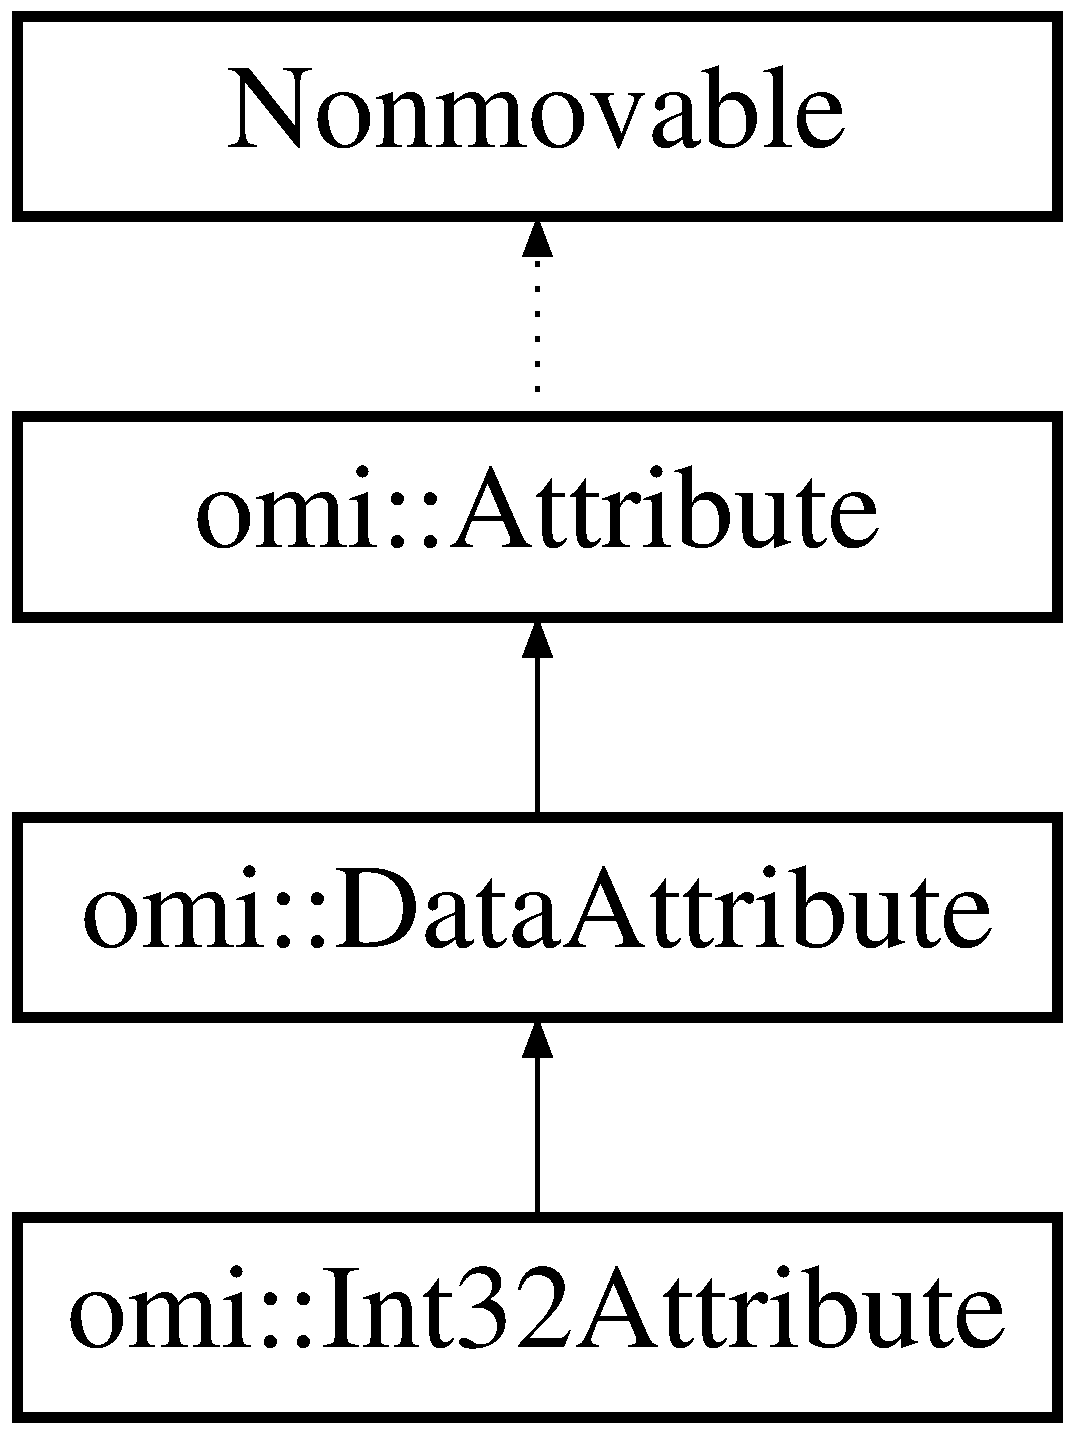
\includegraphics[height=4.000000cm]{classomi_1_1_data_attribute}
\end{center}
\end{figure}
\subsection*{Classes}
\begin{DoxyCompactItemize}
\item 
class \hyperlink{classomi_1_1_data_attribute_1_1_data_storage}{Data\+Storage}
\item 
class \hyperlink{classomi_1_1_data_attribute_1_1_typed_data_storage}{Typed\+Data\+Storage}
\end{DoxyCompactItemize}
\subsection*{Public Member Functions}
\begin{DoxyCompactItemize}
\item 
O\+M\+I\+\_\+\+A\+P\+I\+\_\+\+G\+L\+O\+B\+AL \hyperlink{classomi_1_1_data_attribute_abd881b4d4cecbaa28cffcde63ca64fac}{Data\+Attribute} ()
\begin{DoxyCompactList}\small\item\em Constructs a new null attribute. \end{DoxyCompactList}\item 
O\+M\+I\+\_\+\+A\+P\+I\+\_\+\+G\+L\+O\+B\+AL \hyperlink{classomi_1_1_data_attribute_aedb930a671161cd95858184fd9474e2b}{Data\+Attribute} (const \hyperlink{classomi_1_1_attribute}{Attribute} \&other)
\begin{DoxyCompactList}\small\item\em Constructs a new reference count of the given \hyperlink{classomi_1_1_attribute}{Attribute}. \end{DoxyCompactList}\item 
O\+M\+I\+\_\+\+A\+P\+I\+\_\+\+G\+L\+O\+B\+AL \hyperlink{classomi_1_1_data_attribute_a8b07c9dddb09755e07769eae8a4d4758}{Data\+Attribute} (const \hyperlink{classomi_1_1_data_attribute}{Data\+Attribute} \&other)\hypertarget{classomi_1_1_data_attribute_a8b07c9dddb09755e07769eae8a4d4758}{}\label{classomi_1_1_data_attribute_a8b07c9dddb09755e07769eae8a4d4758}

\begin{DoxyCompactList}\small\item\em Constructs a new reference count of the given \hyperlink{classomi_1_1_data_attribute}{Data\+Attribute}. \end{DoxyCompactList}\item 
O\+M\+I\+\_\+\+A\+P\+I\+\_\+\+G\+L\+O\+B\+AL std\+::size\+\_\+t {\bfseries get\+\_\+size} () const \hypertarget{classomi_1_1_data_attribute_a56a3bc513bdb6669c051136f1e3b39b1}{}\label{classomi_1_1_data_attribute_a56a3bc513bdb6669c051136f1e3b39b1}

\item 
O\+M\+I\+\_\+\+A\+P\+I\+\_\+\+G\+L\+O\+B\+AL std\+::size\+\_\+t {\bfseries get\+\_\+tuple\+\_\+size} () const \hypertarget{classomi_1_1_data_attribute_a1419e9a7c7f81f8178ab9a9d1f5b9925}{}\label{classomi_1_1_data_attribute_a1419e9a7c7f81f8178ab9a9d1f5b9925}

\item 
O\+M\+I\+\_\+\+A\+P\+I\+\_\+\+G\+L\+O\+B\+AL void \hyperlink{classomi_1_1_data_attribute_ae2549b943c913546fa7a85be1e8f6823}{set\+\_\+tuple\+\_\+size} (std\+::size\+\_\+t tuple\+\_\+size)
\begin{DoxyCompactList}\small\item\em Sets the tuple size of this attribute. \end{DoxyCompactList}\end{DoxyCompactItemize}
\subsection*{Static Public Attributes}
\begin{DoxyCompactItemize}
\item 
static \hyperlink{classomi_1_1_attribute_aae4992bc8d2b12679548909bc813eecf}{Type} \hyperlink{classomi_1_1_data_attribute_a643c810debd5ed15523b30b3303f2e07}{k\+Type\+Data\+Bits}\hypertarget{classomi_1_1_data_attribute_a643c810debd5ed15523b30b3303f2e07}{}\label{classomi_1_1_data_attribute_a643c810debd5ed15523b30b3303f2e07}

\begin{DoxyCompactList}\small\item\em In order for an derived type to be considered a valid data attribute the first byte of its type id must be these bits. \end{DoxyCompactList}\end{DoxyCompactItemize}
\subsection*{Protected Member Functions}
\begin{DoxyCompactItemize}
\item 
O\+M\+I\+\_\+\+A\+P\+I\+\_\+\+G\+L\+O\+B\+AL {\bfseries Data\+Attribute} (Definition $\ast$def)\hypertarget{classomi_1_1_data_attribute_acf884a6eab45f04b0cf56a6817bbdbec}{}\label{classomi_1_1_data_attribute_acf884a6eab45f04b0cf56a6817bbdbec}

\item 
O\+M\+I\+\_\+\+A\+P\+I\+\_\+\+G\+L\+O\+B\+AL {\bfseries Data\+Attribute} (\hyperlink{classomi_1_1_attribute_aae4992bc8d2b12679548909bc813eecf}{Type} type, bool immutable, \hyperlink{classomi_1_1_attribute_1_1_storage}{Storage} $\ast$storage)\hypertarget{classomi_1_1_data_attribute_a4f223420e2bf8d2cb80750564e85a27e}{}\label{classomi_1_1_data_attribute_a4f223420e2bf8d2cb80750564e85a27e}

\item 
virtual O\+M\+I\+\_\+\+A\+P\+I\+\_\+\+G\+L\+O\+B\+AL bool \hyperlink{classomi_1_1_data_attribute_a7138ea4cb0415b3da4bdfa813d53fd83}{check\+\_\+type} (\hyperlink{classomi_1_1_attribute_aae4992bc8d2b12679548909bc813eecf}{Type} type) const \hypertarget{classomi_1_1_data_attribute_a7138ea4cb0415b3da4bdfa813d53fd83}{}\label{classomi_1_1_data_attribute_a7138ea4cb0415b3da4bdfa813d53fd83}

\begin{DoxyCompactList}\small\item\em Checks whether the given type is valid for this attribute. \end{DoxyCompactList}\end{DoxyCompactItemize}
\subsection*{Additional Inherited Members}


\subsection{Constructor \& Destructor Documentation}
\index{omi\+::\+Data\+Attribute@{omi\+::\+Data\+Attribute}!Data\+Attribute@{Data\+Attribute}}
\index{Data\+Attribute@{Data\+Attribute}!omi\+::\+Data\+Attribute@{omi\+::\+Data\+Attribute}}
\subsubsection[{\texorpdfstring{Data\+Attribute()}{DataAttribute()}}]{\setlength{\rightskip}{0pt plus 5cm}O\+M\+I\+\_\+\+A\+P\+I\+\_\+\+G\+L\+O\+B\+AL omi\+::\+Data\+Attribute\+::\+Data\+Attribute (
\begin{DoxyParamCaption}
{}
\end{DoxyParamCaption}
)}\hypertarget{classomi_1_1_data_attribute_abd881b4d4cecbaa28cffcde63ca64fac}{}\label{classomi_1_1_data_attribute_abd881b4d4cecbaa28cffcde63ca64fac}


Constructs a new null attribute. 

\begin{DoxyNote}{Note}
This attribute is immutable by definition. 
\end{DoxyNote}
\index{omi\+::\+Data\+Attribute@{omi\+::\+Data\+Attribute}!Data\+Attribute@{Data\+Attribute}}
\index{Data\+Attribute@{Data\+Attribute}!omi\+::\+Data\+Attribute@{omi\+::\+Data\+Attribute}}
\subsubsection[{\texorpdfstring{Data\+Attribute(const Attribute \&other)}{DataAttribute(const Attribute &other)}}]{\setlength{\rightskip}{0pt plus 5cm}O\+M\+I\+\_\+\+A\+P\+I\+\_\+\+G\+L\+O\+B\+AL omi\+::\+Data\+Attribute\+::\+Data\+Attribute (
\begin{DoxyParamCaption}
\item[{const {\bf Attribute} \&}]{other}
\end{DoxyParamCaption}
)}\hypertarget{classomi_1_1_data_attribute_aedb930a671161cd95858184fd9474e2b}{}\label{classomi_1_1_data_attribute_aedb930a671161cd95858184fd9474e2b}


Constructs a new reference count of the given \hyperlink{classomi_1_1_attribute}{Attribute}. 

If the given attribute is not a valid data attribute this construct an invalid \hyperlink{classomi_1_1_data_attribute}{Data\+Attribute}. 

\subsection{Member Function Documentation}
\index{omi\+::\+Data\+Attribute@{omi\+::\+Data\+Attribute}!set\+\_\+tuple\+\_\+size@{set\+\_\+tuple\+\_\+size}}
\index{set\+\_\+tuple\+\_\+size@{set\+\_\+tuple\+\_\+size}!omi\+::\+Data\+Attribute@{omi\+::\+Data\+Attribute}}
\subsubsection[{\texorpdfstring{set\+\_\+tuple\+\_\+size(std\+::size\+\_\+t tuple\+\_\+size)}{set_tuple_size(std::size_t tuple_size)}}]{\setlength{\rightskip}{0pt plus 5cm}O\+M\+I\+\_\+\+A\+P\+I\+\_\+\+G\+L\+O\+B\+AL void omi\+::\+Data\+Attribute\+::set\+\_\+tuple\+\_\+size (
\begin{DoxyParamCaption}
\item[{std\+::size\+\_\+t}]{tuple\+\_\+size}
\end{DoxyParamCaption}
)}\hypertarget{classomi_1_1_data_attribute_ae2549b943c913546fa7a85be1e8f6823}{}\label{classomi_1_1_data_attribute_ae2549b943c913546fa7a85be1e8f6823}


Sets the tuple size of this attribute. 


\begin{DoxyExceptions}{Exceptions}
{\em arc\+::ex\+::\+State\+Error} & If this attribute is not valid. \\
\hline
{\em arc\+::ex\+::\+Illegal\+Action\+Error} & If this attribute is immutable. \\
\hline
\end{DoxyExceptions}


The documentation for this class was generated from the following file\+:\begin{DoxyCompactItemize}
\item 
/home/david/\+Dropbox/\+Development/\+Omicron/\+Omicron/src/cpp/omicron/api/common/attribute/\hyperlink{_data_attribute_8hpp}{Data\+Attribute.\+hpp}\end{DoxyCompactItemize}

\hypertarget{classomi_1_1_data_attribute_1_1_data_storage}{}\section{omi\+:\+:Data\+Attribute\+:\+:Data\+Storage Class Reference}
\label{classomi_1_1_data_attribute_1_1_data_storage}\index{omi\+::\+Data\+Attribute\+::\+Data\+Storage@{omi\+::\+Data\+Attribute\+::\+Data\+Storage}}
Inheritance diagram for omi\+:\+:Data\+Attribute\+:\+:Data\+Storage\+:\begin{figure}[H]
\begin{center}
\leavevmode
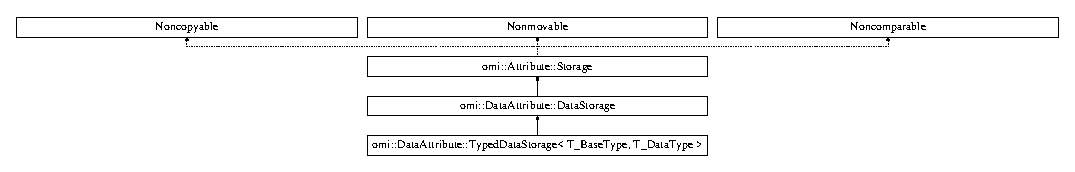
\includegraphics[height=1.866667cm]{classomi_1_1_data_attribute_1_1_data_storage}
\end{center}
\end{figure}
\subsection*{Public Member Functions}
\begin{DoxyCompactItemize}
\item 
O\+M\+I\+\_\+\+A\+P\+I\+\_\+\+G\+L\+O\+B\+AL {\bfseries Data\+Storage} (std\+::size\+\_\+t tuple\+\_\+size)\hypertarget{classomi_1_1_data_attribute_1_1_data_storage_aa3019392c9bb0e5a758fb932bdd81d45}{}\label{classomi_1_1_data_attribute_1_1_data_storage_aa3019392c9bb0e5a758fb932bdd81d45}

\item 
virtual std\+::size\+\_\+t {\bfseries get\+\_\+size} () const =0\hypertarget{classomi_1_1_data_attribute_1_1_data_storage_adf3337bed7c670dbdb96fbf39790df5c}{}\label{classomi_1_1_data_attribute_1_1_data_storage_adf3337bed7c670dbdb96fbf39790df5c}

\end{DoxyCompactItemize}
\subsection*{Public Attributes}
\begin{DoxyCompactItemize}
\item 
std\+::size\+\_\+t {\bfseries m\+\_\+tuple\+\_\+size}\hypertarget{classomi_1_1_data_attribute_1_1_data_storage_aaf014e6b5375b03ca0e666bdde9012b7}{}\label{classomi_1_1_data_attribute_1_1_data_storage_aaf014e6b5375b03ca0e666bdde9012b7}

\end{DoxyCompactItemize}


The documentation for this class was generated from the following file\+:\begin{DoxyCompactItemize}
\item 
/home/david/\+Dropbox/\+Development/\+Omicron/\+Omicron/src/cpp/omicron/api/common/attribute/\hyperlink{_data_attribute_8hpp}{Data\+Attribute.\+hpp}\end{DoxyCompactItemize}

\hypertarget{classomi_1_1runtime_1_1_engine}{}\section{omi\+:\+:runtime\+:\+:Engine Class Reference}
\label{classomi_1_1runtime_1_1_engine}\index{omi\+::runtime\+::\+Engine@{omi\+::runtime\+::\+Engine}}


Singleton object that owns and starts the Omicron runtime.  




{\ttfamily \#include $<$Engine.\+hpp$>$}

Inheritance diagram for omi\+:\+:runtime\+:\+:Engine\+:\begin{figure}[H]
\begin{center}
\leavevmode
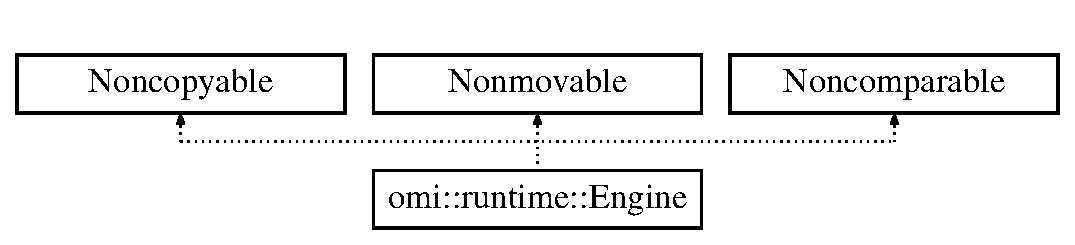
\includegraphics[height=2.000000cm]{classomi_1_1runtime_1_1_engine}
\end{center}
\end{figure}
\subsection*{Public Member Functions}
\begin{DoxyCompactItemize}
\item 
int \hyperlink{classomi_1_1runtime_1_1_engine_add2aeb2865862a1dc5e8b5592cad2e5e}{execute} ()
\begin{DoxyCompactList}\small\item\em Begins execution of Omicron. \end{DoxyCompactList}\item 
bool \hyperlink{classomi_1_1runtime_1_1_engine_ab717cc2830aac8d4816b7d158d1ae9ca}{cycle} ()
\begin{DoxyCompactList}\small\item\em Performs a cycle of execution of the Omicron engine. \end{DoxyCompactList}\end{DoxyCompactItemize}
\subsection*{Static Public Member Functions}
\begin{DoxyCompactItemize}
\item 
static \hyperlink{classomi_1_1runtime_1_1_engine}{Engine} $\ast$ \hyperlink{classomi_1_1runtime_1_1_engine_aadc8b985e369c5f8acf1398cb52c05e9}{instance} ()\hypertarget{classomi_1_1runtime_1_1_engine_aadc8b985e369c5f8acf1398cb52c05e9}{}\label{classomi_1_1runtime_1_1_engine_aadc8b985e369c5f8acf1398cb52c05e9}

\begin{DoxyCompactList}\small\item\em Returns the singleton instance of the Omicron engine. \end{DoxyCompactList}\item 
static bool \hyperlink{classomi_1_1runtime_1_1_engine_a63a594841069c9d544d66f04d758dd38}{cycle\+\_\+static} ()
\begin{DoxyCompactList}\small\item\em Performs a cycle of execution of the Omicron engine. \end{DoxyCompactList}\end{DoxyCompactItemize}


\subsection{Detailed Description}
Singleton object that owns and starts the Omicron runtime. 

\subsection{Member Function Documentation}
\index{omi\+::runtime\+::\+Engine@{omi\+::runtime\+::\+Engine}!cycle\+\_\+static@{cycle\+\_\+static}}
\index{cycle\+\_\+static@{cycle\+\_\+static}!omi\+::runtime\+::\+Engine@{omi\+::runtime\+::\+Engine}}
\subsubsection[{\texorpdfstring{cycle\+\_\+static()}{cycle_static()}}]{\setlength{\rightskip}{0pt plus 5cm}static bool omi\+::runtime\+::\+Engine\+::cycle\+\_\+static (
\begin{DoxyParamCaption}
{}
\end{DoxyParamCaption}
)\hspace{0.3cm}{\ttfamily [static]}}\hypertarget{classomi_1_1runtime_1_1_engine_a63a594841069c9d544d66f04d758dd38}{}\label{classomi_1_1runtime_1_1_engine_a63a594841069c9d544d66f04d758dd38}


Performs a cycle of execution of the Omicron engine. 

Is called by the input subsystem. \index{omi\+::runtime\+::\+Engine@{omi\+::runtime\+::\+Engine}!execute@{execute}}
\index{execute@{execute}!omi\+::runtime\+::\+Engine@{omi\+::runtime\+::\+Engine}}
\subsubsection[{\texorpdfstring{execute()}{execute()}}]{\setlength{\rightskip}{0pt plus 5cm}int omi\+::runtime\+::\+Engine\+::execute (
\begin{DoxyParamCaption}
{}
\end{DoxyParamCaption}
)}\hypertarget{classomi_1_1runtime_1_1_engine_add2aeb2865862a1dc5e8b5592cad2e5e}{}\label{classomi_1_1runtime_1_1_engine_add2aeb2865862a1dc5e8b5592cad2e5e}


Begins execution of Omicron. 

Control is only returned from this function once Omicron exits. \index{omi\+::runtime\+::\+Engine@{omi\+::runtime\+::\+Engine}!cycle@{cycle}}
\index{cycle@{cycle}!omi\+::runtime\+::\+Engine@{omi\+::runtime\+::\+Engine}}
\subsubsection[{\texorpdfstring{cycle()}{cycle()}}]{\setlength{\rightskip}{0pt plus 5cm}bool omi\+::runtime\+::\+Engine\+::cycle (
\begin{DoxyParamCaption}
{}
\end{DoxyParamCaption}
)}\hypertarget{classomi_1_1runtime_1_1_engine_ab717cc2830aac8d4816b7d158d1ae9ca}{}\label{classomi_1_1runtime_1_1_engine_ab717cc2830aac8d4816b7d158d1ae9ca}


Performs a cycle of execution of the Omicron engine. 

Is called by the cycle\+\_\+static function. 

The documentation for this class was generated from the following file\+:\begin{DoxyCompactItemize}
\item 
/home/david/\+Dropbox/\+Development/\+Omicron/\+Omicron/src/cpp/omicron/runtime/\hyperlink{_engine_8hpp}{Engine.\+hpp}\end{DoxyCompactItemize}

\hypertarget{class_frame_buffer}{}\section{Frame\+Buffer Class Reference}
\label{class_frame_buffer}\index{Frame\+Buffer@{Frame\+Buffer}}


Manages and renders the pxtrace framebuffer.  




{\ttfamily \#include $<$Frame\+Buffer.\+hpp$>$}

Inheritance diagram for Frame\+Buffer\+:\begin{figure}[H]
\begin{center}
\leavevmode
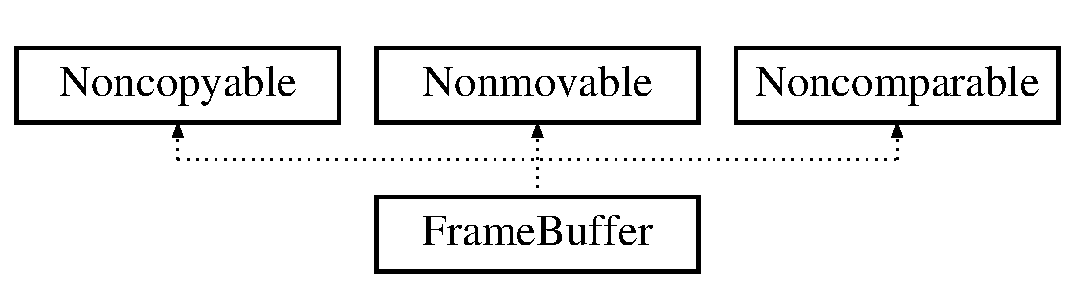
\includegraphics[height=2.000000cm]{class_frame_buffer}
\end{center}
\end{figure}
\subsection*{Public Member Functions}
\begin{DoxyCompactItemize}
\item 
{\bfseries Frame\+Buffer} (const arc\+::gm\+::\+Vector2u \&dimensions)\hypertarget{class_frame_buffer_a401bafe0883b04f8ad3646df6ab8c2f8}{}\label{class_frame_buffer_a401bafe0883b04f8ad3646df6ab8c2f8}

\item 
const arc\+::gm\+::\+Vector2u \& {\bfseries get\+\_\+dimensions} () const \hypertarget{class_frame_buffer_ac2d95d560c78b10f9d4fa6f451f7ae4f}{}\label{class_frame_buffer_ac2d95d560c78b10f9d4fa6f451f7ae4f}

\item 
void {\bfseries clear} (const arc\+::gm\+::\+Vector3f \&colour)\hypertarget{class_frame_buffer_ad483b674420912d9d83e96f9a5a69606}{}\label{class_frame_buffer_ad483b674420912d9d83e96f9a5a69606}

\item 
void {\bfseries set} (const arc\+::gm\+::\+Vector2u \&coords, const arc\+::gm\+::\+Vector3f \&colour)\hypertarget{class_frame_buffer_afef184689769b3c02bafe48925660820}{}\label{class_frame_buffer_afef184689769b3c02bafe48925660820}

\item 
void {\bfseries render} ()\hypertarget{class_frame_buffer_a10f86a6dc0649d660a17fc184a7dcc27}{}\label{class_frame_buffer_a10f86a6dc0649d660a17fc184a7dcc27}

\end{DoxyCompactItemize}


\subsection{Detailed Description}
Manages and renders the pxtrace framebuffer. 

The documentation for this class was generated from the following file\+:\begin{DoxyCompactItemize}
\item 
/home/david/\+Dropbox/\+Development/\+Omicron/\+Omicron/src/cpp/builtin\+\_\+subsystems/pxtrace/\hyperlink{_frame_buffer_8hpp}{Frame\+Buffer.\+hpp}\end{DoxyCompactItemize}

\hypertarget{classomi_1_1asset_1_1_geometry}{}\section{omi\+:\+:asset\+:\+:Geometry Class Reference}
\label{classomi_1_1asset_1_1_geometry}\index{omi\+::asset\+::\+Geometry@{omi\+::asset\+::\+Geometry}}
Inheritance diagram for omi\+:\+:asset\+:\+:Geometry\+:\begin{figure}[H]
\begin{center}
\leavevmode
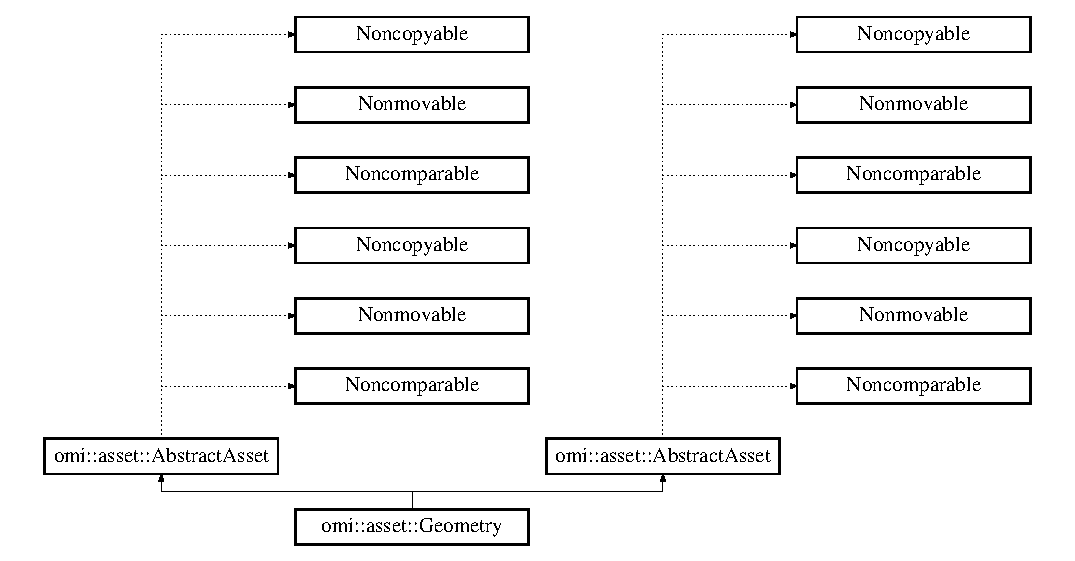
\includegraphics[height=7.088607cm]{classomi_1_1asset_1_1_geometry}
\end{center}
\end{figure}
\subsection*{Classes}
\begin{DoxyCompactItemize}
\item 
class \hyperlink{classomi_1_1asset_1_1_geometry_1_1_resource}{Resource}
\end{DoxyCompactItemize}


The documentation for this class was generated from the following file\+:\begin{DoxyCompactItemize}
\item 
/home/david/\+Dropbox/\+Development/\+Omicron/\+Omicron/src/cpp/omicron/api/asset/types/bk/\hyperlink{_geometry_asset_8hpp}{Geometry\+Asset.\+hpp}\end{DoxyCompactItemize}

\hypertarget{classomi__gl_1_1_g_l_bootstrap}{}\section{omi\+\_\+gl\+:\+:G\+L\+Bootstrap Class Reference}
\label{classomi__gl_1_1_g_l_bootstrap}\index{omi\+\_\+gl\+::\+G\+L\+Bootstrap@{omi\+\_\+gl\+::\+G\+L\+Bootstrap}}


Handles startup and shutdown of the Omicron GL rendering subsystem.  




{\ttfamily \#include $<$G\+L\+Bootstrap.\+hpp$>$}

Inheritance diagram for omi\+\_\+gl\+:\+:G\+L\+Bootstrap\+:\begin{figure}[H]
\begin{center}
\leavevmode
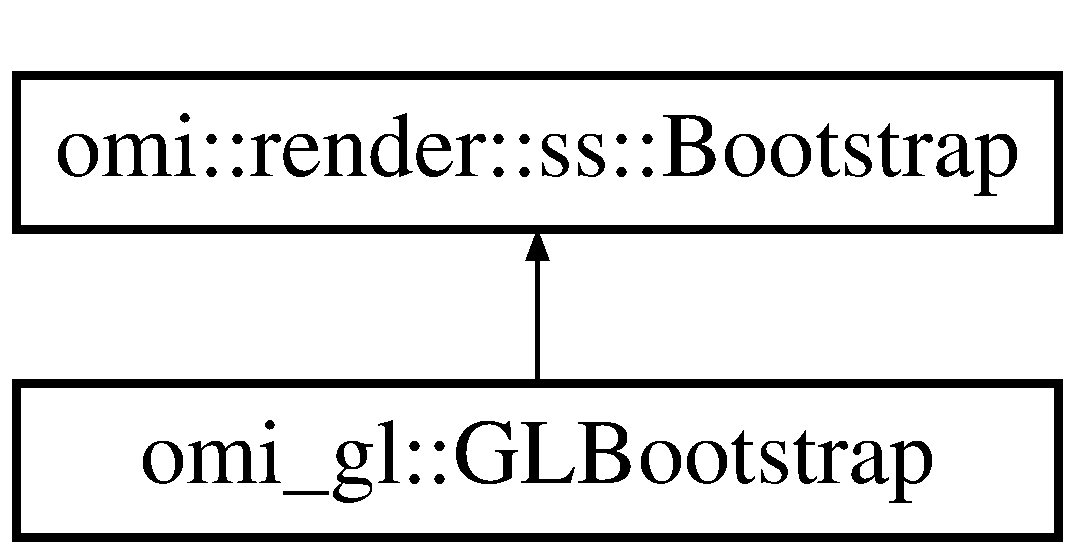
\includegraphics[height=2.000000cm]{classomi__gl_1_1_g_l_bootstrap}
\end{center}
\end{figure}
\subsection*{Public Member Functions}
\begin{DoxyCompactItemize}
\item 
virtual void \hyperlink{classomi__gl_1_1_g_l_bootstrap_a2cb4f9ea291138b1fb0943a6957f89c5}{startup} ()
\begin{DoxyCompactList}\small\item\em Starts up this Omicron rendering subsystem. \end{DoxyCompactList}\item 
virtual void \hyperlink{classomi__gl_1_1_g_l_bootstrap_ae086f372b2f8e5b56087bb28c4310d14}{shutdown} ()
\begin{DoxyCompactList}\small\item\em Starts up this Omicron rendering subsystem. \end{DoxyCompactList}\end{DoxyCompactItemize}
\subsection*{Static Public Member Functions}
\begin{DoxyCompactItemize}
\item 
static \hyperlink{classomi__gl_1_1_g_l_bootstrap}{G\+L\+Bootstrap} $\ast$ \hyperlink{classomi__gl_1_1_g_l_bootstrap_a953189805951f06b681396675965bb12}{get\+\_\+instance} ()\hypertarget{classomi__gl_1_1_g_l_bootstrap_a953189805951f06b681396675965bb12}{}\label{classomi__gl_1_1_g_l_bootstrap_a953189805951f06b681396675965bb12}

\begin{DoxyCompactList}\small\item\em Returns the singleton instance of the Omicron GL bootstrapper. \end{DoxyCompactList}\end{DoxyCompactItemize}
\subsection*{Additional Inherited Members}


\subsection{Detailed Description}
Handles startup and shutdown of the Omicron GL rendering subsystem. 

\subsection{Member Function Documentation}
\index{omi\+\_\+gl\+::\+G\+L\+Bootstrap@{omi\+\_\+gl\+::\+G\+L\+Bootstrap}!startup@{startup}}
\index{startup@{startup}!omi\+\_\+gl\+::\+G\+L\+Bootstrap@{omi\+\_\+gl\+::\+G\+L\+Bootstrap}}
\subsubsection[{\texorpdfstring{startup()}{startup()}}]{\setlength{\rightskip}{0pt plus 5cm}virtual void omi\+\_\+gl\+::\+G\+L\+Bootstrap\+::startup (
\begin{DoxyParamCaption}
{}
\end{DoxyParamCaption}
)\hspace{0.3cm}{\ttfamily [virtual]}}\hypertarget{classomi__gl_1_1_g_l_bootstrap_a2cb4f9ea291138b1fb0943a6957f89c5}{}\label{classomi__gl_1_1_g_l_bootstrap_a2cb4f9ea291138b1fb0943a6957f89c5}


Starts up this Omicron rendering subsystem. 

Other than the Bootstrap\textquotesingle{}s constructor this will be the first call made to this object, and will only be made once. 

Reimplemented from \hyperlink{classomi_1_1render_1_1ss_1_1_bootstrap_a3b7e12774f56ce17baee150c5c85e1cb}{omi\+::render\+::ss\+::\+Bootstrap}.

\index{omi\+\_\+gl\+::\+G\+L\+Bootstrap@{omi\+\_\+gl\+::\+G\+L\+Bootstrap}!shutdown@{shutdown}}
\index{shutdown@{shutdown}!omi\+\_\+gl\+::\+G\+L\+Bootstrap@{omi\+\_\+gl\+::\+G\+L\+Bootstrap}}
\subsubsection[{\texorpdfstring{shutdown()}{shutdown()}}]{\setlength{\rightskip}{0pt plus 5cm}virtual void omi\+\_\+gl\+::\+G\+L\+Bootstrap\+::shutdown (
\begin{DoxyParamCaption}
{}
\end{DoxyParamCaption}
)\hspace{0.3cm}{\ttfamily [virtual]}}\hypertarget{classomi__gl_1_1_g_l_bootstrap_ae086f372b2f8e5b56087bb28c4310d14}{}\label{classomi__gl_1_1_g_l_bootstrap_ae086f372b2f8e5b56087bb28c4310d14}


Starts up this Omicron rendering subsystem. 

Other than the Bootstrap\textquotesingle{}s destructor this will be the last call made to this object, and will only be made once. 

Reimplemented from \hyperlink{classomi_1_1render_1_1ss_1_1_bootstrap_af4f13ba4968f7dac6141a7c558188aaf}{omi\+::render\+::ss\+::\+Bootstrap}.



The documentation for this class was generated from the following file\+:\begin{DoxyCompactItemize}
\item 
/home/david/\+Dropbox/\+Development/\+Omicron/\+Omicron/src/cpp/builtin\+\_\+subsystems/omi\+\_\+gl/\hyperlink{_g_l_bootstrap_8hpp}{G\+L\+Bootstrap.\+hpp}\end{DoxyCompactItemize}

\hypertarget{class_g_l_subsystem}{}\section{G\+L\+Subsystem Class Reference}
\label{class_g_l_subsystem}\index{G\+L\+Subsystem@{G\+L\+Subsystem}}


T\+O\+DO.  




{\ttfamily \#include $<$G\+L\+Subsystem.\+hpp$>$}

Inheritance diagram for G\+L\+Subsystem\+:\begin{figure}[H]
\begin{center}
\leavevmode
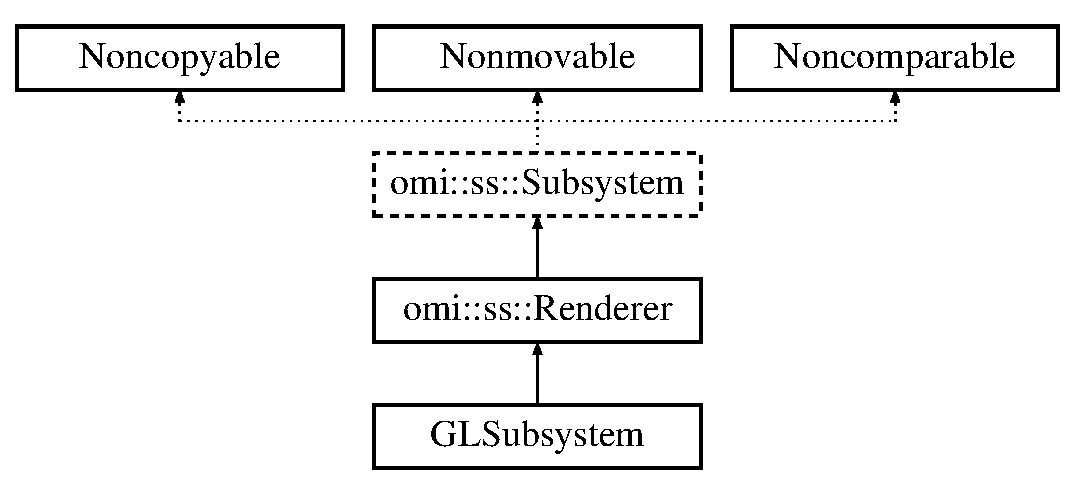
\includegraphics[height=4.000000cm]{class_g_l_subsystem}
\end{center}
\end{figure}
\subsection*{Public Member Functions}
\begin{DoxyCompactItemize}
\item 
virtual void \hyperlink{class_g_l_subsystem_a05c8c799107f035e4effe8b55edbe16d}{startup} ()
\begin{DoxyCompactList}\small\item\em Startups up this subsystem. \end{DoxyCompactList}\item 
virtual void \hyperlink{class_g_l_subsystem_ab158d7f38b073a986714a02c10606abc}{setup\+\_\+rendering} ()\hypertarget{class_g_l_subsystem_ab158d7f38b073a986714a02c10606abc}{}\label{class_g_l_subsystem_ab158d7f38b073a986714a02c10606abc}

\begin{DoxyCompactList}\small\item\em Is called once a valid GL context has been established to setup rendering. \end{DoxyCompactList}\item 
virtual void \hyperlink{class_g_l_subsystem_a542f9685fe4b2924aec576fd836e51e1}{render} ()\hypertarget{class_g_l_subsystem_a542f9685fe4b2924aec576fd836e51e1}{}\label{class_g_l_subsystem_a542f9685fe4b2924aec576fd836e51e1}

\begin{DoxyCompactList}\small\item\em Is called to render the current frame. \end{DoxyCompactList}\end{DoxyCompactItemize}
\subsection*{Additional Inherited Members}


\subsection{Detailed Description}
T\+O\+DO. 

\subsection{Member Function Documentation}
\index{G\+L\+Subsystem@{G\+L\+Subsystem}!startup@{startup}}
\index{startup@{startup}!G\+L\+Subsystem@{G\+L\+Subsystem}}
\subsubsection[{\texorpdfstring{startup()}{startup()}}]{\setlength{\rightskip}{0pt plus 5cm}virtual void G\+L\+Subsystem\+::startup (
\begin{DoxyParamCaption}
{}
\end{DoxyParamCaption}
)\hspace{0.3cm}{\ttfamily [virtual]}}\hypertarget{class_g_l_subsystem_a05c8c799107f035e4effe8b55edbe16d}{}\label{class_g_l_subsystem_a05c8c799107f035e4effe8b55edbe16d}


Startups up this subsystem. 

\begin{DoxyWarning}{Warning}
This function should not be called manually.
\end{DoxyWarning}
Other than the constructor, this will be the first call made to this object, and will only be called once. 

Reimplemented from \hyperlink{classomi_1_1ss_1_1_subsystem_a4b0ea0b6a120c551d73151f0e0432197}{omi\+::ss\+::\+Subsystem}.



The documentation for this class was generated from the following file\+:\begin{DoxyCompactItemize}
\item 
/home/david/\+Dropbox/\+Development/\+Omicron/\+Omicron/src/cpp/builtin\+\_\+subsystems/omi\+\_\+gl/\hyperlink{_g_l_subsystem_8hpp}{G\+L\+Subsystem.\+hpp}\end{DoxyCompactItemize}

\hypertarget{classomi_1_1xform_1_1_hierarchical_constraint}{}\section{omi\+:\+:xform\+:\+:Hierarchical\+Constraint Class Reference}
\label{classomi_1_1xform_1_1_hierarchical_constraint}\index{omi\+::xform\+::\+Hierarchical\+Constraint@{omi\+::xform\+::\+Hierarchical\+Constraint}}


T\+O\+DO\+:  




{\ttfamily \#include $<$Hierarchical\+Constraint.\+hpp$>$}

Inheritance diagram for omi\+:\+:xform\+:\+:Hierarchical\+Constraint\+:\begin{figure}[H]
\begin{center}
\leavevmode
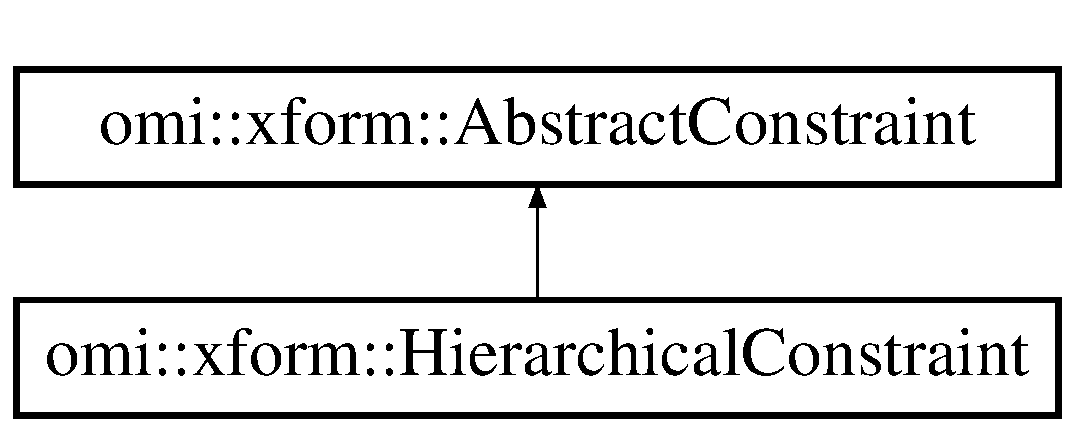
\includegraphics[height=2.000000cm]{classomi_1_1xform_1_1_hierarchical_constraint}
\end{center}
\end{figure}


\subsection{Detailed Description}
T\+O\+DO\+: 

The documentation for this class was generated from the following file\+:\begin{DoxyCompactItemize}
\item 
/home/david/\+Dropbox/\+Development/\+Omicron/\+Omicron/src/cpp/omicron/api/xform/\hyperlink{_hierarchical_constraint_8hpp}{Hierarchical\+Constraint.\+hpp}\end{DoxyCompactItemize}

\hypertarget{classomi_1_1ss_1_1_input}{}\section{omi\+:\+:ss\+:\+:Input Class Reference}
\label{classomi_1_1ss_1_1_input}\index{omi\+::ss\+::\+Input@{omi\+::ss\+::\+Input}}


T\+O\+DO\+:  




{\ttfamily \#include $<$Input.\+hpp$>$}

Inheritance diagram for omi\+:\+:ss\+:\+:Input\+:\begin{figure}[H]
\begin{center}
\leavevmode
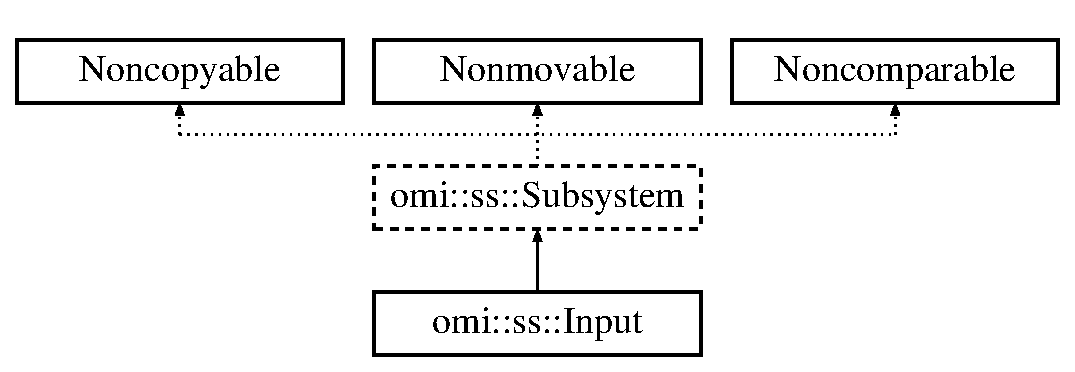
\includegraphics[height=3.000000cm]{classomi_1_1ss_1_1_input}
\end{center}
\end{figure}
\subsection*{Public Types}
\begin{DoxyCompactItemize}
\item 
typedef bool($\ast$ {\bfseries Engine\+Cycle\+Func}) ()\hypertarget{classomi_1_1ss_1_1_input_a335476b6a5ee96900ce2de73f0624077}{}\label{classomi_1_1ss_1_1_input_a335476b6a5ee96900ce2de73f0624077}

\end{DoxyCompactItemize}
\subsection*{Public Member Functions}
\begin{DoxyCompactItemize}
\item 
\hyperlink{classomi_1_1ss_1_1_input_ace2801947529de88eef5ca404f471103}{Input} ()\hypertarget{classomi_1_1ss_1_1_input_ace2801947529de88eef5ca404f471103}{}\label{classomi_1_1ss_1_1_input_ace2801947529de88eef5ca404f471103}

\begin{DoxyCompactList}\small\item\em T\+O\+DO\+: \end{DoxyCompactList}\item 
virtual void \hyperlink{classomi_1_1ss_1_1_input_a6a75340edb3f75ee4318f66905ddab0a}{start\+\_\+main\+\_\+loop} (Engine\+Cycle\+Func engine\+\_\+cycle)=0
\begin{DoxyCompactList}\small\item\em Is called to start the \hyperlink{classomi_1_1ss_1_1_input}{Input} subsystem\textquotesingle{}s main loop. \end{DoxyCompactList}\end{DoxyCompactItemize}
\subsection*{Additional Inherited Members}


\subsection{Detailed Description}
T\+O\+DO\+: 

\subsection{Member Function Documentation}
\index{omi\+::ss\+::\+Input@{omi\+::ss\+::\+Input}!start\+\_\+main\+\_\+loop@{start\+\_\+main\+\_\+loop}}
\index{start\+\_\+main\+\_\+loop@{start\+\_\+main\+\_\+loop}!omi\+::ss\+::\+Input@{omi\+::ss\+::\+Input}}
\subsubsection[{\texorpdfstring{start\+\_\+main\+\_\+loop(\+Engine\+Cycle\+Func engine\+\_\+cycle)=0}{start_main_loop(EngineCycleFunc engine_cycle)=0}}]{\setlength{\rightskip}{0pt plus 5cm}virtual void omi\+::ss\+::\+Input\+::start\+\_\+main\+\_\+loop (
\begin{DoxyParamCaption}
\item[{Engine\+Cycle\+Func}]{engine\+\_\+cycle}
\end{DoxyParamCaption}
)\hspace{0.3cm}{\ttfamily [pure virtual]}}\hypertarget{classomi_1_1ss_1_1_input_a6a75340edb3f75ee4318f66905ddab0a}{}\label{classomi_1_1ss_1_1_input_a6a75340edb3f75ee4318f66905ddab0a}


Is called to start the \hyperlink{classomi_1_1ss_1_1_input}{Input} subsystem\textquotesingle{}s main loop. 


\begin{DoxyParams}{Parameters}
{\em engine\+\_\+cycle} & A function which will execute a cycle of the Omicron engine. This function should be called once every cycle of the \hyperlink{classomi_1_1ss_1_1_input}{Input} subsystem\textquotesingle{}s main loop. This function will return false when engine execution has completed which signals this function should return control. \\
\hline
\end{DoxyParams}


The documentation for this class was generated from the following file\+:\begin{DoxyCompactItemize}
\item 
/home/david/\+Dropbox/\+Development/\+Omicron/\+Omicron/src/cpp/omicron/subsystem/\hyperlink{_input_8hpp}{Input.\+hpp}\end{DoxyCompactItemize}

\hypertarget{classomi_1_1_int32_attribute}{}\section{omi\+:\+:Int32\+Attribute Class Reference}
\label{classomi_1_1_int32_attribute}\index{omi\+::\+Int32\+Attribute@{omi\+::\+Int32\+Attribute}}
Inheritance diagram for omi\+:\+:Int32\+Attribute\+:\begin{figure}[H]
\begin{center}
\leavevmode
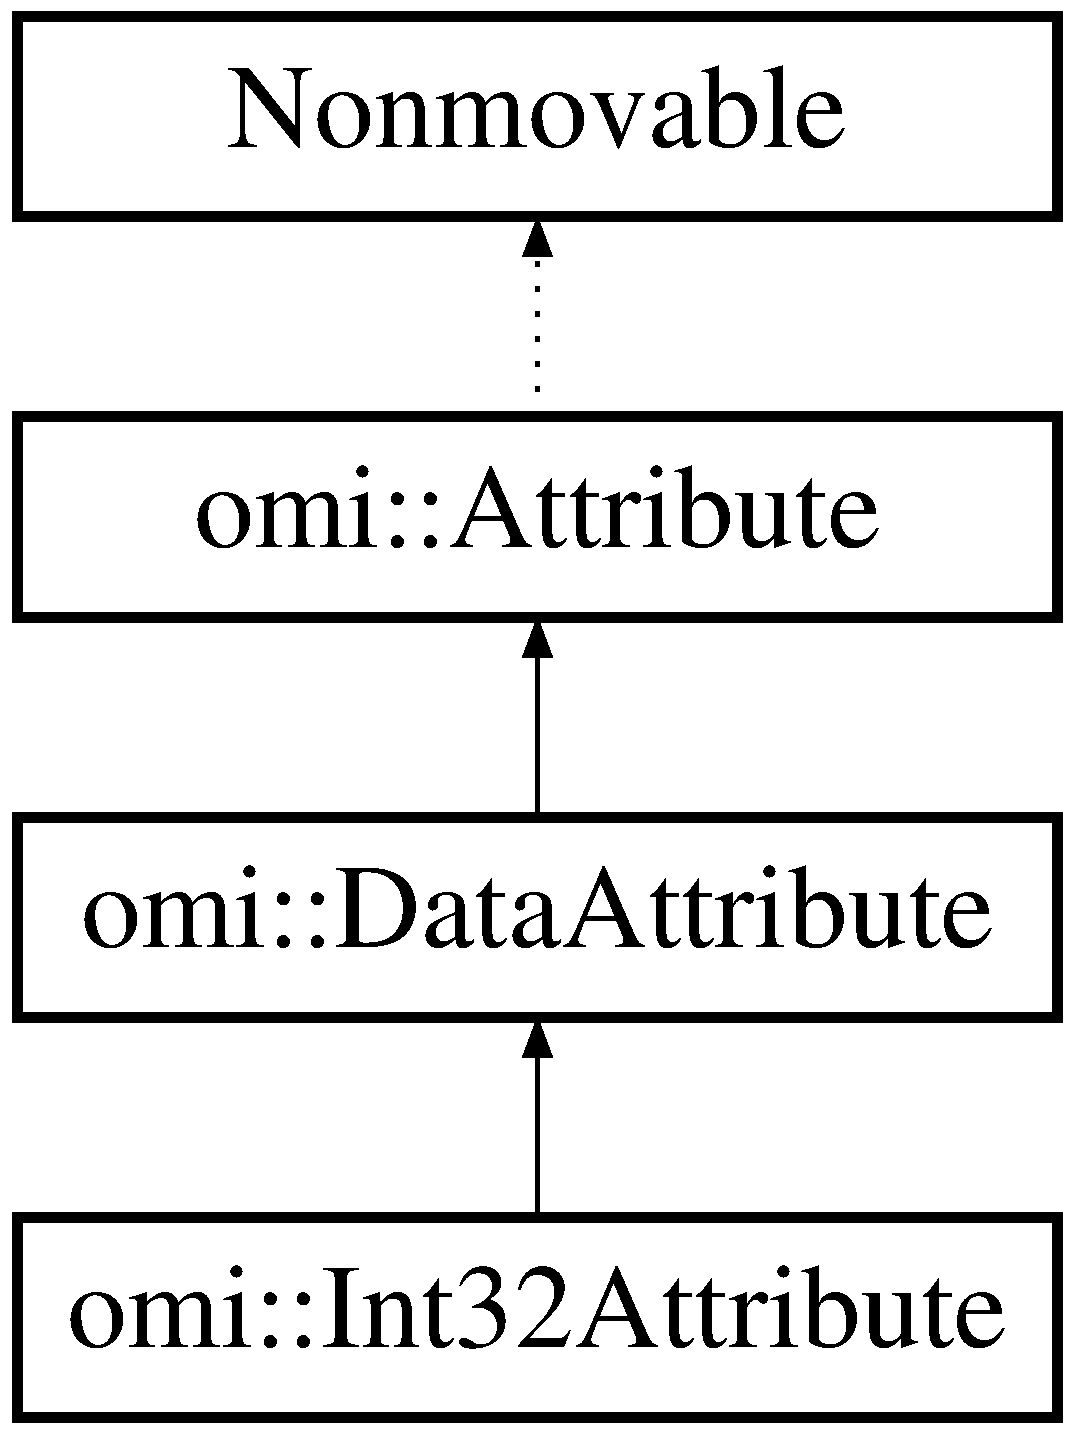
\includegraphics[height=4.000000cm]{classomi_1_1_int32_attribute}
\end{center}
\end{figure}
\subsection*{Public Types}
\begin{DoxyCompactItemize}
\item 
typedef arc\+::int32 \hyperlink{classomi_1_1_int32_attribute_aaafef3adcf9a0111695451449dfa1a2d}{Data\+Type}\hypertarget{classomi_1_1_int32_attribute_aaafef3adcf9a0111695451449dfa1a2d}{}\label{classomi_1_1_int32_attribute_aaafef3adcf9a0111695451449dfa1a2d}

\begin{DoxyCompactList}\small\item\em The data type this attribute is storing. \end{DoxyCompactList}\item 
typedef std\+::vector$<$ \hyperlink{classomi_1_1_int32_attribute_aaafef3adcf9a0111695451449dfa1a2d}{Data\+Type} $>$ \hyperlink{classomi_1_1_int32_attribute_a09ae7167f71512dc47ef34d96bf3baf5}{Array\+Type}\hypertarget{classomi_1_1_int32_attribute_a09ae7167f71512dc47ef34d96bf3baf5}{}\label{classomi_1_1_int32_attribute_a09ae7167f71512dc47ef34d96bf3baf5}

\begin{DoxyCompactList}\small\item\em The array type that is used to return weak references to this attribute\textquotesingle{}s data. \end{DoxyCompactList}\item 
typedef \hyperlink{classomi_1_1_data_attribute_1_1_typed_data_storage}{Data\+Attribute\+::\+Typed\+Data\+Storage}$<$ \hyperlink{classomi_1_1_int32_attribute}{Int32\+Attribute}, \hyperlink{classomi_1_1_int32_attribute_aaafef3adcf9a0111695451449dfa1a2d}{Data\+Type} $>$ {\bfseries Int32\+Storage}\hypertarget{classomi_1_1_int32_attribute_ae3fe389bff1926ad7327338433ac05d9}{}\label{classomi_1_1_int32_attribute_ae3fe389bff1926ad7327338433ac05d9}

\end{DoxyCompactItemize}
\subsection*{Public Member Functions}
\begin{DoxyCompactItemize}
\item 
O\+M\+I\+\_\+\+A\+P\+I\+\_\+\+G\+L\+O\+B\+AL \hyperlink{classomi_1_1_int32_attribute_a3563bd9594cc4e47ae4eb6501446eedc}{Int32\+Attribute} (bool immutable=true)
\begin{DoxyCompactList}\small\item\em Constructs a new empty int32 attribute. \end{DoxyCompactList}\item 
O\+M\+I\+\_\+\+A\+P\+I\+\_\+\+G\+L\+O\+B\+AL {\bfseries Int32\+Attribute} (\hyperlink{classomi_1_1_int32_attribute_aaafef3adcf9a0111695451449dfa1a2d}{Data\+Type} value, bool immutable=true)\hypertarget{classomi_1_1_int32_attribute_a5ad7c9cd6d42c54e7cc2d26c181a29e9}{}\label{classomi_1_1_int32_attribute_a5ad7c9cd6d42c54e7cc2d26c181a29e9}

\item 
{\footnotesize template$<$typename T\+\_\+\+Input\+Iterator $>$ }\\{\bfseries Int32\+Attribute} (const T\+\_\+\+Input\+Iterator \&first, const T\+\_\+\+Input\+Iterator \&last, std\+::size\+\_\+t tuple\+\_\+size=0, bool immutable=true)\hypertarget{classomi_1_1_int32_attribute_a39539919b93afb3d49c60c2954322447}{}\label{classomi_1_1_int32_attribute_a39539919b93afb3d49c60c2954322447}

\item 
O\+M\+I\+\_\+\+A\+P\+I\+\_\+\+G\+L\+O\+B\+AL {\bfseries Int32\+Attribute} (const \hyperlink{classomi_1_1_int32_attribute_a09ae7167f71512dc47ef34d96bf3baf5}{Array\+Type} \&values, std\+::size\+\_\+t tuple\+\_\+size=0, bool immutable=true)\hypertarget{classomi_1_1_int32_attribute_a5586139ca5a4a48c5364394a265bdeb0}{}\label{classomi_1_1_int32_attribute_a5586139ca5a4a48c5364394a265bdeb0}

\item 
O\+M\+I\+\_\+\+A\+P\+I\+\_\+\+G\+L\+O\+B\+AL \hyperlink{classomi_1_1_int32_attribute_a6c21c2c18daeebed6391be7995cc3d79}{Int32\+Attribute} (const \hyperlink{classomi_1_1_attribute}{Attribute} \&other)
\begin{DoxyCompactList}\small\item\em Constructs a new reference count of the given \hyperlink{classomi_1_1_attribute}{Attribute}. \end{DoxyCompactList}\item 
O\+M\+I\+\_\+\+A\+P\+I\+\_\+\+G\+L\+O\+B\+AL \hyperlink{classomi_1_1_int32_attribute_a93e4103db7d56ca756d54a74bbb15c3c}{Int32\+Attribute} (const \hyperlink{classomi_1_1_int32_attribute}{Int32\+Attribute} \&other)
\begin{DoxyCompactList}\small\item\em Constructs a new reference count of the given attribute. \end{DoxyCompactList}\item 
O\+M\+I\+\_\+\+A\+P\+I\+\_\+\+G\+L\+O\+B\+AL \hyperlink{classomi_1_1_int32_attribute_aaafef3adcf9a0111695451449dfa1a2d}{Data\+Type} \hyperlink{classomi_1_1_int32_attribute_af82dc5de2c62769fa8e26c7350439c1a}{get\+\_\+value} () const 
\begin{DoxyCompactList}\small\item\em Returns the first integer value of this attribute. \end{DoxyCompactList}\item 
O\+M\+I\+\_\+\+A\+P\+I\+\_\+\+G\+L\+O\+B\+AL const \hyperlink{classomi_1_1_int32_attribute_a09ae7167f71512dc47ef34d96bf3baf5}{Array\+Type} \& \hyperlink{classomi_1_1_int32_attribute_adeaec7b2ca620a28155f0c18e25a0fed}{get\+\_\+values} () const 
\begin{DoxyCompactList}\small\item\em Returns the array of values of this attribute. \end{DoxyCompactList}\item 
O\+M\+I\+\_\+\+A\+P\+I\+\_\+\+G\+L\+O\+B\+AL void \hyperlink{classomi_1_1_int32_attribute_afae23b709686441ca374a25c09d124db}{set\+\_\+value} (\hyperlink{classomi_1_1_int32_attribute_aaafef3adcf9a0111695451449dfa1a2d}{Data\+Type} value)
\begin{DoxyCompactList}\small\item\em Sets the value of this attribute to be a size 1 array holding the given value. \end{DoxyCompactList}\item 
{\footnotesize template$<$typename T\+\_\+\+Input\+Iterator $>$ }\\void \hyperlink{classomi_1_1_int32_attribute_ab6bc4bba2260a2952e4c3e4629bebcb2}{set\+\_\+values} (const T\+\_\+\+Input\+Iterator \&first, const T\+\_\+\+Input\+Iterator \&last)
\begin{DoxyCompactList}\small\item\em Sets the value of this attribute to be a copy of the array specified by the first and last (one past the end) iterators. \end{DoxyCompactList}\item 
O\+M\+I\+\_\+\+A\+P\+I\+\_\+\+G\+L\+O\+B\+AL void \hyperlink{classomi_1_1_int32_attribute_a1863bba4dc4d71a3d919d804c8e1a1de}{set\+\_\+values} (const \hyperlink{classomi_1_1_int32_attribute_a09ae7167f71512dc47ef34d96bf3baf5}{Array\+Type} \&values)
\begin{DoxyCompactList}\small\item\em Sets the value of this attribute to be a copy of the data within the given vector. \end{DoxyCompactList}\end{DoxyCompactItemize}
\subsection*{Static Public Member Functions}
\begin{DoxyCompactItemize}
\item 
static O\+M\+I\+\_\+\+A\+P\+I\+\_\+\+G\+L\+O\+B\+AL arc\+::str\+::\+U\+T\+F8\+String {\bfseries get\+\_\+type\+\_\+string} ()\hypertarget{classomi_1_1_int32_attribute_a7c4650bf0ff46163f7c85532bebc6fe3}{}\label{classomi_1_1_int32_attribute_a7c4650bf0ff46163f7c85532bebc6fe3}

\end{DoxyCompactItemize}
\subsection*{Static Public Attributes}
\begin{DoxyCompactItemize}
\item 
static O\+M\+I\+\_\+\+A\+P\+I\+\_\+\+G\+L\+O\+B\+AL \hyperlink{classomi_1_1_attribute_aae4992bc8d2b12679548909bc813eecf}{Type} \hyperlink{classomi_1_1_int32_attribute_aff60d30ef7b90e9bd02631f74d0f0d94}{k\+Type\+Int32}\hypertarget{classomi_1_1_int32_attribute_aff60d30ef7b90e9bd02631f74d0f0d94}{}\label{classomi_1_1_int32_attribute_aff60d30ef7b90e9bd02631f74d0f0d94}

\begin{DoxyCompactList}\small\item\em The type identifier for int32 attributes. \end{DoxyCompactList}\end{DoxyCompactItemize}
\subsection*{Protected Member Functions}
\begin{DoxyCompactItemize}
\item 
virtual O\+M\+I\+\_\+\+A\+P\+I\+\_\+\+G\+L\+O\+B\+AL bool \hyperlink{classomi_1_1_int32_attribute_a00405334d8a08a2af74078e2d9ce4d9b}{check\+\_\+type} (\hyperlink{classomi_1_1_attribute_aae4992bc8d2b12679548909bc813eecf}{Type} type) const \hypertarget{classomi_1_1_int32_attribute_a00405334d8a08a2af74078e2d9ce4d9b}{}\label{classomi_1_1_int32_attribute_a00405334d8a08a2af74078e2d9ce4d9b}

\begin{DoxyCompactList}\small\item\em Checks whether the given type is valid for this attribute. \end{DoxyCompactList}\end{DoxyCompactItemize}


\subsection{Constructor \& Destructor Documentation}
\index{omi\+::\+Int32\+Attribute@{omi\+::\+Int32\+Attribute}!Int32\+Attribute@{Int32\+Attribute}}
\index{Int32\+Attribute@{Int32\+Attribute}!omi\+::\+Int32\+Attribute@{omi\+::\+Int32\+Attribute}}
\subsubsection[{\texorpdfstring{Int32\+Attribute(bool immutable=true)}{Int32Attribute(bool immutable=true)}}]{\setlength{\rightskip}{0pt plus 5cm}O\+M\+I\+\_\+\+A\+P\+I\+\_\+\+G\+L\+O\+B\+AL omi\+::\+Int32\+Attribute\+::\+Int32\+Attribute (
\begin{DoxyParamCaption}
\item[{bool}]{immutable = {\ttfamily true}}
\end{DoxyParamCaption}
)}\hypertarget{classomi_1_1_int32_attribute_a3563bd9594cc4e47ae4eb6501446eedc}{}\label{classomi_1_1_int32_attribute_a3563bd9594cc4e47ae4eb6501446eedc}


Constructs a new empty int32 attribute. 


\begin{DoxyParams}{Parameters}
{\em immutable} & Whether this attribute is immutable or not. \\
\hline
\end{DoxyParams}
\index{omi\+::\+Int32\+Attribute@{omi\+::\+Int32\+Attribute}!Int32\+Attribute@{Int32\+Attribute}}
\index{Int32\+Attribute@{Int32\+Attribute}!omi\+::\+Int32\+Attribute@{omi\+::\+Int32\+Attribute}}
\subsubsection[{\texorpdfstring{Int32\+Attribute(const Attribute \&other)}{Int32Attribute(const Attribute &other)}}]{\setlength{\rightskip}{0pt plus 5cm}O\+M\+I\+\_\+\+A\+P\+I\+\_\+\+G\+L\+O\+B\+AL omi\+::\+Int32\+Attribute\+::\+Int32\+Attribute (
\begin{DoxyParamCaption}
\item[{const {\bf Attribute} \&}]{other}
\end{DoxyParamCaption}
)}\hypertarget{classomi_1_1_int32_attribute_a6c21c2c18daeebed6391be7995cc3d79}{}\label{classomi_1_1_int32_attribute_a6c21c2c18daeebed6391be7995cc3d79}


Constructs a new reference count of the given \hyperlink{classomi_1_1_attribute}{Attribute}. 

If the given attribute is not a valid int32 attribute this will construct a null attribute and the reference count will not be increased. \index{omi\+::\+Int32\+Attribute@{omi\+::\+Int32\+Attribute}!Int32\+Attribute@{Int32\+Attribute}}
\index{Int32\+Attribute@{Int32\+Attribute}!omi\+::\+Int32\+Attribute@{omi\+::\+Int32\+Attribute}}
\subsubsection[{\texorpdfstring{Int32\+Attribute(const Int32\+Attribute \&other)}{Int32Attribute(const Int32Attribute &other)}}]{\setlength{\rightskip}{0pt plus 5cm}O\+M\+I\+\_\+\+A\+P\+I\+\_\+\+G\+L\+O\+B\+AL omi\+::\+Int32\+Attribute\+::\+Int32\+Attribute (
\begin{DoxyParamCaption}
\item[{const {\bf Int32\+Attribute} \&}]{other}
\end{DoxyParamCaption}
)}\hypertarget{classomi_1_1_int32_attribute_a93e4103db7d56ca756d54a74bbb15c3c}{}\label{classomi_1_1_int32_attribute_a93e4103db7d56ca756d54a74bbb15c3c}


Constructs a new reference count of the given attribute. 

If the given attribute is invalid this will construct a null attribute and the reference count will not be increased. 

\subsection{Member Function Documentation}
\index{omi\+::\+Int32\+Attribute@{omi\+::\+Int32\+Attribute}!get\+\_\+value@{get\+\_\+value}}
\index{get\+\_\+value@{get\+\_\+value}!omi\+::\+Int32\+Attribute@{omi\+::\+Int32\+Attribute}}
\subsubsection[{\texorpdfstring{get\+\_\+value() const }{get_value() const }}]{\setlength{\rightskip}{0pt plus 5cm}O\+M\+I\+\_\+\+A\+P\+I\+\_\+\+G\+L\+O\+B\+AL {\bf Data\+Type} omi\+::\+Int32\+Attribute\+::get\+\_\+value (
\begin{DoxyParamCaption}
{}
\end{DoxyParamCaption}
) const}\hypertarget{classomi_1_1_int32_attribute_af82dc5de2c62769fa8e26c7350439c1a}{}\label{classomi_1_1_int32_attribute_af82dc5de2c62769fa8e26c7350439c1a}


Returns the first integer value of this attribute. 


\begin{DoxyExceptions}{Exceptions}
{\em arc\+::ex\+::\+State\+Error} & If this attribute is not valid. \\
\hline
{\em arc\+::ex\+::\+Index\+Out\+Of\+Bounds\+Error} & If this attribute has no values. \\
\hline
\end{DoxyExceptions}
\index{omi\+::\+Int32\+Attribute@{omi\+::\+Int32\+Attribute}!get\+\_\+values@{get\+\_\+values}}
\index{get\+\_\+values@{get\+\_\+values}!omi\+::\+Int32\+Attribute@{omi\+::\+Int32\+Attribute}}
\subsubsection[{\texorpdfstring{get\+\_\+values() const }{get_values() const }}]{\setlength{\rightskip}{0pt plus 5cm}O\+M\+I\+\_\+\+A\+P\+I\+\_\+\+G\+L\+O\+B\+AL const {\bf Array\+Type}\& omi\+::\+Int32\+Attribute\+::get\+\_\+values (
\begin{DoxyParamCaption}
{}
\end{DoxyParamCaption}
) const}\hypertarget{classomi_1_1_int32_attribute_adeaec7b2ca620a28155f0c18e25a0fed}{}\label{classomi_1_1_int32_attribute_adeaec7b2ca620a28155f0c18e25a0fed}


Returns the array of values of this attribute. 


\begin{DoxyExceptions}{Exceptions}
{\em arc\+::ex\+::\+State\+Error} & If this attribute is not valid. \\
\hline
\end{DoxyExceptions}
\index{omi\+::\+Int32\+Attribute@{omi\+::\+Int32\+Attribute}!set\+\_\+value@{set\+\_\+value}}
\index{set\+\_\+value@{set\+\_\+value}!omi\+::\+Int32\+Attribute@{omi\+::\+Int32\+Attribute}}
\subsubsection[{\texorpdfstring{set\+\_\+value(\+Data\+Type value)}{set_value(DataType value)}}]{\setlength{\rightskip}{0pt plus 5cm}O\+M\+I\+\_\+\+A\+P\+I\+\_\+\+G\+L\+O\+B\+AL void omi\+::\+Int32\+Attribute\+::set\+\_\+value (
\begin{DoxyParamCaption}
\item[{{\bf Data\+Type}}]{value}
\end{DoxyParamCaption}
)}\hypertarget{classomi_1_1_int32_attribute_afae23b709686441ca374a25c09d124db}{}\label{classomi_1_1_int32_attribute_afae23b709686441ca374a25c09d124db}


Sets the value of this attribute to be a size 1 array holding the given value. 


\begin{DoxyExceptions}{Exceptions}
{\em arc\+::ex\+::\+State\+Error} & If this attribute is not valid. \\
\hline
{\em arc\+::ex\+::\+Illegal\+Action\+Error} & If this attribute is immutable. \\
\hline
\end{DoxyExceptions}
\index{omi\+::\+Int32\+Attribute@{omi\+::\+Int32\+Attribute}!set\+\_\+values@{set\+\_\+values}}
\index{set\+\_\+values@{set\+\_\+values}!omi\+::\+Int32\+Attribute@{omi\+::\+Int32\+Attribute}}
\subsubsection[{\texorpdfstring{set\+\_\+values(const T\+\_\+\+Input\+Iterator \&first, const T\+\_\+\+Input\+Iterator \&last)}{set_values(const T_InputIterator &first, const T_InputIterator &last)}}]{\setlength{\rightskip}{0pt plus 5cm}template$<$typename T\+\_\+\+Input\+Iterator $>$ void omi\+::\+Int32\+Attribute\+::set\+\_\+values (
\begin{DoxyParamCaption}
\item[{const T\+\_\+\+Input\+Iterator \&}]{first, }
\item[{const T\+\_\+\+Input\+Iterator \&}]{last}
\end{DoxyParamCaption}
)\hspace{0.3cm}{\ttfamily [inline]}}\hypertarget{classomi_1_1_int32_attribute_ab6bc4bba2260a2952e4c3e4629bebcb2}{}\label{classomi_1_1_int32_attribute_ab6bc4bba2260a2952e4c3e4629bebcb2}


Sets the value of this attribute to be a copy of the array specified by the first and last (one past the end) iterators. 


\begin{DoxyExceptions}{Exceptions}
{\em arc\+::ex\+::\+State\+Error} & If this attribute is not valid. \\
\hline
{\em arc\+::ex\+::\+Illegal\+Action\+Error} & If this attribute is immutable. \\
\hline
\end{DoxyExceptions}
\index{omi\+::\+Int32\+Attribute@{omi\+::\+Int32\+Attribute}!set\+\_\+values@{set\+\_\+values}}
\index{set\+\_\+values@{set\+\_\+values}!omi\+::\+Int32\+Attribute@{omi\+::\+Int32\+Attribute}}
\subsubsection[{\texorpdfstring{set\+\_\+values(const Array\+Type \&values)}{set_values(const ArrayType &values)}}]{\setlength{\rightskip}{0pt plus 5cm}O\+M\+I\+\_\+\+A\+P\+I\+\_\+\+G\+L\+O\+B\+AL void omi\+::\+Int32\+Attribute\+::set\+\_\+values (
\begin{DoxyParamCaption}
\item[{const {\bf Array\+Type} \&}]{values}
\end{DoxyParamCaption}
)}\hypertarget{classomi_1_1_int32_attribute_a1863bba4dc4d71a3d919d804c8e1a1de}{}\label{classomi_1_1_int32_attribute_a1863bba4dc4d71a3d919d804c8e1a1de}


Sets the value of this attribute to be a copy of the data within the given vector. 


\begin{DoxyExceptions}{Exceptions}
{\em arc\+::ex\+::\+State\+Error} & If this attribute is not valid. \\
\hline
{\em arc\+::ex\+::\+Illegal\+Action\+Error} & If this attribute is immutable. \\
\hline
\end{DoxyExceptions}


The documentation for this class was generated from the following file\+:\begin{DoxyCompactItemize}
\item 
/home/david/\+Dropbox/\+Development/\+Omicron/\+Omicron/src/cpp/omicron/api/common/attribute/\hyperlink{_int32_attribute_8hpp}{Int32\+Attribute.\+hpp}\end{DoxyCompactItemize}

\hypertarget{classomi_1_1window_1_1_main_window}{}\section{omi\+:\+:window\+:\+:Main\+Window Class Reference}
\label{classomi_1_1window_1_1_main_window}\index{omi\+::window\+::\+Main\+Window@{omi\+::window\+::\+Main\+Window}}


Singleton object which controls the main window of Omicron.  




{\ttfamily \#include $<$Main\+Window.\+hpp$>$}

Inheritance diagram for omi\+:\+:window\+:\+:Main\+Window\+:\begin{figure}[H]
\begin{center}
\leavevmode
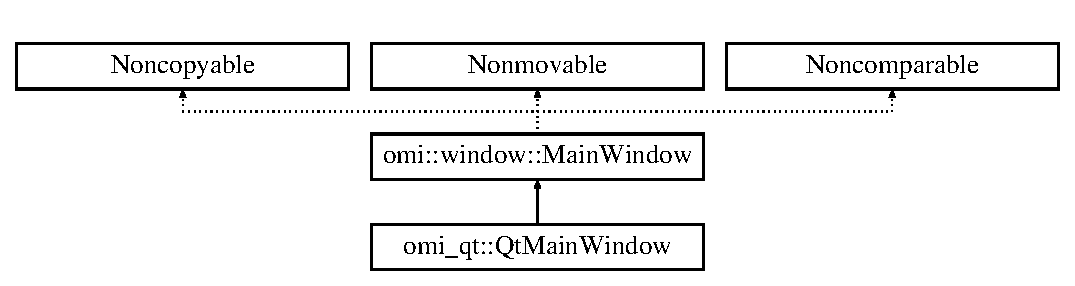
\includegraphics[height=3.000000cm]{classomi_1_1window_1_1_main_window}
\end{center}
\end{figure}
\subsection*{Public Member Functions}
\begin{DoxyCompactItemize}
\item 
virtual \hyperlink{namespaceomi_1_1window_a096dc3d82796b93c067bca535fc0f94e}{Window\+Mode} \hyperlink{classomi_1_1window_1_1_main_window_a79b2016501c95af6cdd66df0277773fb}{get\+\_\+mode} () const =0\hypertarget{classomi_1_1window_1_1_main_window_a79b2016501c95af6cdd66df0277773fb}{}\label{classomi_1_1window_1_1_main_window_a79b2016501c95af6cdd66df0277773fb}

\begin{DoxyCompactList}\small\item\em Returns the current windowing mode of the main window. \end{DoxyCompactList}\item 
virtual void \hyperlink{classomi_1_1window_1_1_main_window_aea247b966ad921d2107d8b64b751735d}{set\+\_\+mode} (\hyperlink{namespaceomi_1_1window_a096dc3d82796b93c067bca535fc0f94e}{Window\+Mode} mode)=0\hypertarget{classomi_1_1window_1_1_main_window_aea247b966ad921d2107d8b64b751735d}{}\label{classomi_1_1window_1_1_main_window_aea247b966ad921d2107d8b64b751735d}

\begin{DoxyCompactList}\small\item\em Sets the windowing mode the main window will use. \end{DoxyCompactList}\end{DoxyCompactItemize}
\subsection*{Static Public Member Functions}
\begin{DoxyCompactItemize}
\item 
static O\+M\+I\+\_\+\+A\+P\+I\+\_\+\+G\+L\+O\+B\+AL \hyperlink{classomi_1_1window_1_1_main_window}{Main\+Window} $\ast$ \hyperlink{classomi_1_1window_1_1_main_window_a70da804588730859dd1227cee0c2e6c5}{instance} ()\hypertarget{classomi_1_1window_1_1_main_window_a70da804588730859dd1227cee0c2e6c5}{}\label{classomi_1_1window_1_1_main_window_a70da804588730859dd1227cee0c2e6c5}

\begin{DoxyCompactList}\small\item\em Returns the singleton instance of the main window. \end{DoxyCompactList}\end{DoxyCompactItemize}


\subsection{Detailed Description}
Singleton object which controls the main window of Omicron. 

The documentation for this class was generated from the following file\+:\begin{DoxyCompactItemize}
\item 
/home/david/\+Dropbox/\+Development/\+Omicron/\+Omicron/src/cpp/omicron/api/window/\hyperlink{_main_window_8hpp}{Main\+Window.\+hpp}\end{DoxyCompactItemize}

\hypertarget{classomi_1_1_map_attribute}{}\section{omi\+:\+:Map\+Attribute Class Reference}
\label{classomi_1_1_map_attribute}\index{omi\+::\+Map\+Attribute@{omi\+::\+Map\+Attribute}}
Inheritance diagram for omi\+:\+:Map\+Attribute\+:\begin{figure}[H]
\begin{center}
\leavevmode
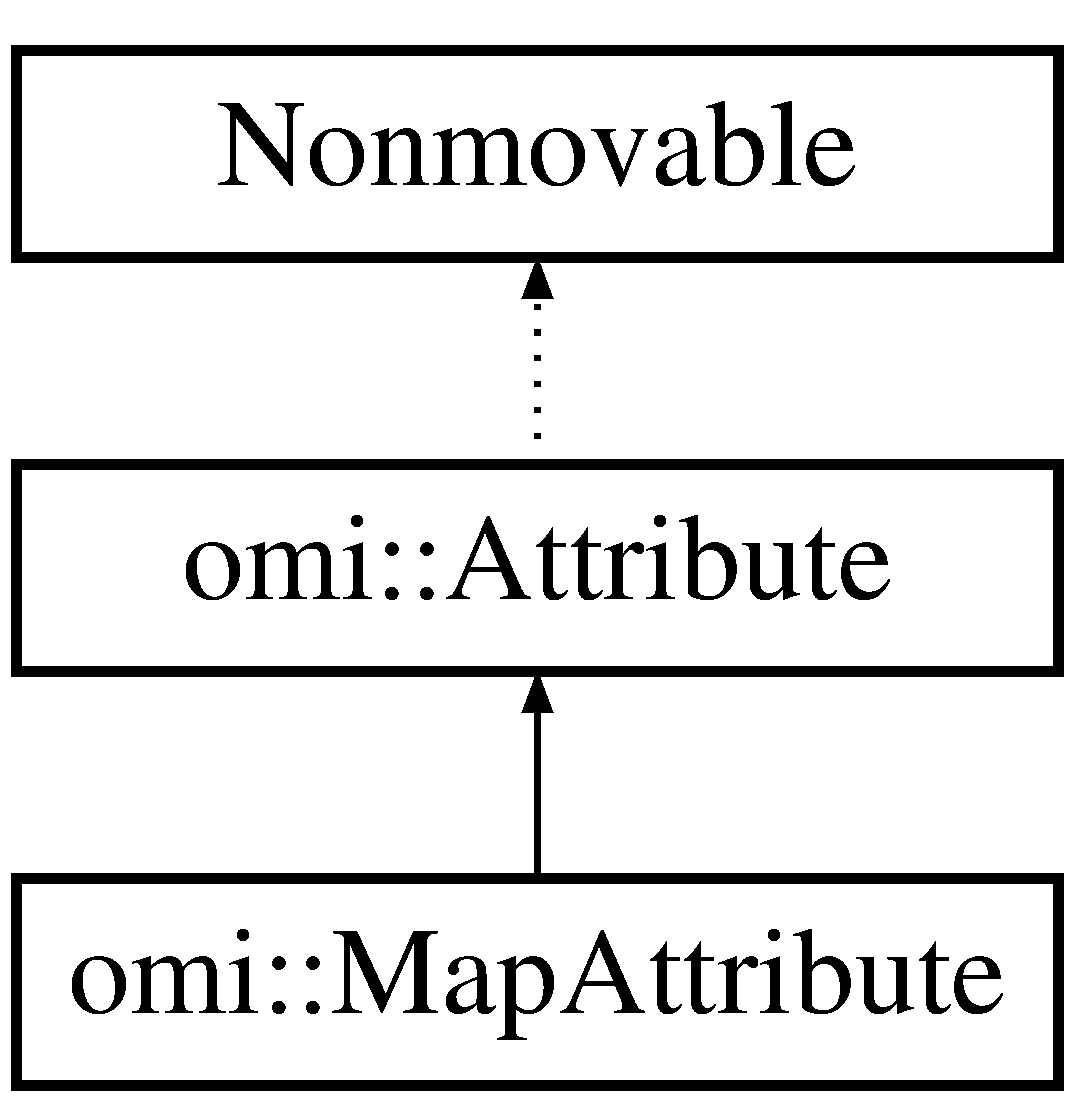
\includegraphics[height=3.000000cm]{classomi_1_1_map_attribute}
\end{center}
\end{figure}
\subsection*{Classes}
\begin{DoxyCompactItemize}
\item 
class \hyperlink{classomi_1_1_map_attribute_1_1_map_storage}{Map\+Storage}
\end{DoxyCompactItemize}
\subsection*{Public Types}
\begin{DoxyCompactItemize}
\item 
typedef std\+::map$<$ arc\+::str\+::\+U\+T\+F8\+String, \hyperlink{classomi_1_1_attribute}{Attribute} $>$ \hyperlink{classomi_1_1_map_attribute_ac5a11b90e684944a18bcd18376d7eed1}{Data\+Type}\hypertarget{classomi_1_1_map_attribute_ac5a11b90e684944a18bcd18376d7eed1}{}\label{classomi_1_1_map_attribute_ac5a11b90e684944a18bcd18376d7eed1}

\begin{DoxyCompactList}\small\item\em The type used to store \hyperlink{classomi_1_1_map_attribute}{Map\+Attribute}\textquotesingle{}s data. \end{DoxyCompactList}\end{DoxyCompactItemize}
\subsection*{Public Member Functions}
\begin{DoxyCompactItemize}
\item 
O\+M\+I\+\_\+\+A\+P\+I\+\_\+\+G\+L\+O\+B\+AL \hyperlink{classomi_1_1_map_attribute_a5c2fc5c4bf83db0d7d9f7b06c1d022d9}{Map\+Attribute} (bool immutable=true)
\begin{DoxyCompactList}\small\item\em Constructs a new empty \hyperlink{classomi_1_1_map_attribute}{Map\+Attribute}. \end{DoxyCompactList}\item 
{\footnotesize template$<$typename T\+\_\+\+Input\+Iterator $>$ }\\{\bfseries Map\+Attribute} (const T\+\_\+\+Input\+Iterator \&first, const T\+\_\+\+Input\+Iterator \&last, bool immutable=true)\hypertarget{classomi_1_1_map_attribute_a7b4361cdb47fda693aac20424b9f0450}{}\label{classomi_1_1_map_attribute_a7b4361cdb47fda693aac20424b9f0450}

\item 
O\+M\+I\+\_\+\+A\+P\+I\+\_\+\+G\+L\+O\+B\+AL {\bfseries Map\+Attribute} (const \hyperlink{classomi_1_1_map_attribute_ac5a11b90e684944a18bcd18376d7eed1}{Data\+Type} \&data, bool immutable=true)\hypertarget{classomi_1_1_map_attribute_a4a8ff9223a0cc5584995fc7b5048d839}{}\label{classomi_1_1_map_attribute_a4a8ff9223a0cc5584995fc7b5048d839}

\item 
O\+M\+I\+\_\+\+A\+P\+I\+\_\+\+G\+L\+O\+B\+AL \hyperlink{classomi_1_1_map_attribute_a05936738a93a13b8fda8a38fa6e5791f}{Map\+Attribute} (const \hyperlink{classomi_1_1_attribute}{Attribute} \&other)
\begin{DoxyCompactList}\small\item\em Constructs a new reference count of the given \hyperlink{classomi_1_1_attribute}{Attribute}. \end{DoxyCompactList}\item 
O\+M\+I\+\_\+\+A\+P\+I\+\_\+\+G\+L\+O\+B\+AL \hyperlink{classomi_1_1_map_attribute_a84bc4aedd43fa24e278d7bc0bd39d7e4}{Map\+Attribute} (const \hyperlink{classomi_1_1_map_attribute}{Map\+Attribute} \&other)
\begin{DoxyCompactList}\small\item\em Constructs a new reference count of the given \hyperlink{classomi_1_1_attribute}{Attribute}. \end{DoxyCompactList}\item 
O\+M\+I\+\_\+\+A\+P\+I\+\_\+\+G\+L\+O\+B\+AL std\+::size\+\_\+t \hyperlink{classomi_1_1_map_attribute_a3c3118f3575100288c189c21f4dc566d}{get\+\_\+size} () const 
\begin{DoxyCompactList}\small\item\em Returns the number of entries in this \hyperlink{classomi_1_1_map_attribute}{Map\+Attribute}. \end{DoxyCompactList}\item 
O\+M\+I\+\_\+\+A\+P\+I\+\_\+\+G\+L\+O\+B\+AL const \hyperlink{classomi_1_1_map_attribute_ac5a11b90e684944a18bcd18376d7eed1}{Data\+Type} \& \hyperlink{classomi_1_1_map_attribute_a8370199919959e84e1f981375a3bb5f0}{get\+\_\+data} () const 
\begin{DoxyCompactList}\small\item\em Returns the internal map structure of this \hyperlink{classomi_1_1_map_attribute}{Map\+Attribute}. \end{DoxyCompactList}\item 
O\+M\+I\+\_\+\+A\+P\+I\+\_\+\+G\+L\+O\+B\+AL std\+::vector$<$ arc\+::str\+::\+U\+T\+F8\+String $>$ \hyperlink{classomi_1_1_map_attribute_a2b61b6c28fa25d1879e7711138055466}{get\+\_\+names} () const 
\begin{DoxyCompactList}\small\item\em Returns the names (keys) of the entries in this \hyperlink{classomi_1_1_map_attribute}{Map\+Attribute}. \end{DoxyCompactList}\item 
O\+M\+I\+\_\+\+A\+P\+I\+\_\+\+G\+L\+O\+B\+AL std\+::vector$<$ \hyperlink{classomi_1_1_attribute}{Attribute} $>$ \hyperlink{classomi_1_1_map_attribute_a600ec6e7edb7fde8529340cb65f3861f}{get\+\_\+attributes} () const 
\begin{DoxyCompactList}\small\item\em Returns the attributes (values) of the entries in this \hyperlink{classomi_1_1_map_attribute}{Map\+Attribute}. \end{DoxyCompactList}\item 
O\+M\+I\+\_\+\+A\+P\+I\+\_\+\+G\+L\+O\+B\+AL bool \hyperlink{classomi_1_1_map_attribute_ac1c6c017c7068f08e1d9fbbe926f171b}{has} (const arc\+::str\+::\+U\+T\+F8\+String \&name) const 
\begin{DoxyCompactList}\small\item\em Returns whether there is an entry in the map with the given name. \end{DoxyCompactList}\item 
O\+M\+I\+\_\+\+A\+P\+I\+\_\+\+G\+L\+O\+B\+AL const \hyperlink{classomi_1_1_attribute}{Attribute} \& \hyperlink{classomi_1_1_map_attribute_a65d78eb8f9b4ab89989c164986ae638b}{get} (const arc\+::str\+::\+U\+T\+F8\+String \&name) const 
\begin{DoxyCompactList}\small\item\em Returns the attribute in this \hyperlink{classomi_1_1_map_attribute}{Map\+Attribute} under the given name. \end{DoxyCompactList}\item 
O\+M\+I\+\_\+\+A\+P\+I\+\_\+\+G\+L\+O\+B\+AL void \hyperlink{classomi_1_1_map_attribute_a38565aee85f4bdb82792aa368b459e95}{insert} (const arc\+::str\+::\+U\+T\+F8\+String \&name, const \hyperlink{classomi_1_1_attribute}{Attribute} \&attrribute)
\begin{DoxyCompactList}\small\item\em Inserts the given attribute into the map under the provided name. \end{DoxyCompactList}\item 
O\+M\+I\+\_\+\+A\+P\+I\+\_\+\+G\+L\+O\+B\+AL void \hyperlink{classomi_1_1_map_attribute_abed8fa17cdd3ce28b95471c947f3701d}{erase} (const arc\+::str\+::\+U\+T\+F8\+String \&name)
\begin{DoxyCompactList}\small\item\em Removes the attribute with the given name from this \hyperlink{classomi_1_1_map_attribute}{Map\+Attribute}. \end{DoxyCompactList}\item 
{\footnotesize template$<$typename T\+\_\+\+Input\+Iterator $>$ }\\void \hyperlink{classomi_1_1_map_attribute_a301205039db6d6446920b6394f00e61a}{set\+\_\+data} (const T\+\_\+\+Input\+Iterator \&first, const T\+\_\+\+Input\+Iterator \&last)
\begin{DoxyCompactList}\small\item\em Replaces the current data of this \hyperlink{classomi_1_1_map_attribute}{Map\+Attribute} with the given data. \end{DoxyCompactList}\item 
O\+M\+I\+\_\+\+A\+P\+I\+\_\+\+G\+L\+O\+B\+AL void \hyperlink{classomi_1_1_map_attribute_a91f57783b4f26e58d980c5af53e6d1ca}{set\+\_\+data} (const \hyperlink{classomi_1_1_map_attribute_ac5a11b90e684944a18bcd18376d7eed1}{Data\+Type} \&data)
\begin{DoxyCompactList}\small\item\em Replaces the current data of this \hyperlink{classomi_1_1_map_attribute}{Map\+Attribute} with the given data. \end{DoxyCompactList}\item 
O\+M\+I\+\_\+\+A\+P\+I\+\_\+\+G\+L\+O\+B\+AL void \hyperlink{classomi_1_1_map_attribute_aa1c68fdaa6b87ea72bdd34889293b944}{clear} ()
\begin{DoxyCompactList}\small\item\em Clears the contents of this \hyperlink{classomi_1_1_map_attribute}{Map\+Attribute} -\/ effectively replacing the current data with empty data. \end{DoxyCompactList}\end{DoxyCompactItemize}
\subsection*{Static Public Attributes}
\begin{DoxyCompactItemize}
\item 
static O\+M\+I\+\_\+\+A\+P\+I\+\_\+\+G\+L\+O\+B\+AL \hyperlink{classomi_1_1_attribute_aae4992bc8d2b12679548909bc813eecf}{Type} \hyperlink{classomi_1_1_map_attribute_a2d55813e6394bea0e8e7ba00880a963b}{k\+Type\+Map}\hypertarget{classomi_1_1_map_attribute_a2d55813e6394bea0e8e7ba00880a963b}{}\label{classomi_1_1_map_attribute_a2d55813e6394bea0e8e7ba00880a963b}

\begin{DoxyCompactList}\small\item\em The type identifier for map attributes. \end{DoxyCompactList}\end{DoxyCompactItemize}
\subsection*{Additional Inherited Members}


\subsection{Constructor \& Destructor Documentation}
\index{omi\+::\+Map\+Attribute@{omi\+::\+Map\+Attribute}!Map\+Attribute@{Map\+Attribute}}
\index{Map\+Attribute@{Map\+Attribute}!omi\+::\+Map\+Attribute@{omi\+::\+Map\+Attribute}}
\subsubsection[{\texorpdfstring{Map\+Attribute(bool immutable=true)}{MapAttribute(bool immutable=true)}}]{\setlength{\rightskip}{0pt plus 5cm}O\+M\+I\+\_\+\+A\+P\+I\+\_\+\+G\+L\+O\+B\+AL omi\+::\+Map\+Attribute\+::\+Map\+Attribute (
\begin{DoxyParamCaption}
\item[{bool}]{immutable = {\ttfamily true}}
\end{DoxyParamCaption}
)}\hypertarget{classomi_1_1_map_attribute_a5c2fc5c4bf83db0d7d9f7b06c1d022d9}{}\label{classomi_1_1_map_attribute_a5c2fc5c4bf83db0d7d9f7b06c1d022d9}


Constructs a new empty \hyperlink{classomi_1_1_map_attribute}{Map\+Attribute}. 


\begin{DoxyParams}{Parameters}
{\em immutable} & Whether this attribute is immutable or not. \\
\hline
\end{DoxyParams}
\index{omi\+::\+Map\+Attribute@{omi\+::\+Map\+Attribute}!Map\+Attribute@{Map\+Attribute}}
\index{Map\+Attribute@{Map\+Attribute}!omi\+::\+Map\+Attribute@{omi\+::\+Map\+Attribute}}
\subsubsection[{\texorpdfstring{Map\+Attribute(const Attribute \&other)}{MapAttribute(const Attribute &other)}}]{\setlength{\rightskip}{0pt plus 5cm}O\+M\+I\+\_\+\+A\+P\+I\+\_\+\+G\+L\+O\+B\+AL omi\+::\+Map\+Attribute\+::\+Map\+Attribute (
\begin{DoxyParamCaption}
\item[{const {\bf Attribute} \&}]{other}
\end{DoxyParamCaption}
)}\hypertarget{classomi_1_1_map_attribute_a05936738a93a13b8fda8a38fa6e5791f}{}\label{classomi_1_1_map_attribute_a05936738a93a13b8fda8a38fa6e5791f}


Constructs a new reference count of the given \hyperlink{classomi_1_1_attribute}{Attribute}. 

If the given attribute is not a valid map attribute this will construct a null attribute and the reference count will not be increased. \index{omi\+::\+Map\+Attribute@{omi\+::\+Map\+Attribute}!Map\+Attribute@{Map\+Attribute}}
\index{Map\+Attribute@{Map\+Attribute}!omi\+::\+Map\+Attribute@{omi\+::\+Map\+Attribute}}
\subsubsection[{\texorpdfstring{Map\+Attribute(const Map\+Attribute \&other)}{MapAttribute(const MapAttribute &other)}}]{\setlength{\rightskip}{0pt plus 5cm}O\+M\+I\+\_\+\+A\+P\+I\+\_\+\+G\+L\+O\+B\+AL omi\+::\+Map\+Attribute\+::\+Map\+Attribute (
\begin{DoxyParamCaption}
\item[{const {\bf Map\+Attribute} \&}]{other}
\end{DoxyParamCaption}
)}\hypertarget{classomi_1_1_map_attribute_a84bc4aedd43fa24e278d7bc0bd39d7e4}{}\label{classomi_1_1_map_attribute_a84bc4aedd43fa24e278d7bc0bd39d7e4}


Constructs a new reference count of the given \hyperlink{classomi_1_1_attribute}{Attribute}. 

If the given attribute is invalid this will construct a null attribute and the reference count will not be increased. 

\subsection{Member Function Documentation}
\index{omi\+::\+Map\+Attribute@{omi\+::\+Map\+Attribute}!get\+\_\+size@{get\+\_\+size}}
\index{get\+\_\+size@{get\+\_\+size}!omi\+::\+Map\+Attribute@{omi\+::\+Map\+Attribute}}
\subsubsection[{\texorpdfstring{get\+\_\+size() const }{get_size() const }}]{\setlength{\rightskip}{0pt plus 5cm}O\+M\+I\+\_\+\+A\+P\+I\+\_\+\+G\+L\+O\+B\+AL std\+::size\+\_\+t omi\+::\+Map\+Attribute\+::get\+\_\+size (
\begin{DoxyParamCaption}
{}
\end{DoxyParamCaption}
) const}\hypertarget{classomi_1_1_map_attribute_a3c3118f3575100288c189c21f4dc566d}{}\label{classomi_1_1_map_attribute_a3c3118f3575100288c189c21f4dc566d}


Returns the number of entries in this \hyperlink{classomi_1_1_map_attribute}{Map\+Attribute}. 


\begin{DoxyExceptions}{Exceptions}
{\em arc\+::ex\+::\+State\+Error} & If this attribute is not valid. \\
\hline
\end{DoxyExceptions}
\index{omi\+::\+Map\+Attribute@{omi\+::\+Map\+Attribute}!get\+\_\+data@{get\+\_\+data}}
\index{get\+\_\+data@{get\+\_\+data}!omi\+::\+Map\+Attribute@{omi\+::\+Map\+Attribute}}
\subsubsection[{\texorpdfstring{get\+\_\+data() const }{get_data() const }}]{\setlength{\rightskip}{0pt plus 5cm}O\+M\+I\+\_\+\+A\+P\+I\+\_\+\+G\+L\+O\+B\+AL const {\bf Data\+Type}\& omi\+::\+Map\+Attribute\+::get\+\_\+data (
\begin{DoxyParamCaption}
{}
\end{DoxyParamCaption}
) const}\hypertarget{classomi_1_1_map_attribute_a8370199919959e84e1f981375a3bb5f0}{}\label{classomi_1_1_map_attribute_a8370199919959e84e1f981375a3bb5f0}


Returns the internal map structure of this \hyperlink{classomi_1_1_map_attribute}{Map\+Attribute}. 

\begin{DoxyNote}{Note}
Using this structure is this fastest way to iterator over the contents of this attribute.
\end{DoxyNote}

\begin{DoxyExceptions}{Exceptions}
{\em arc\+::ex\+::\+State\+Error} & If this attribute is not valid. \\
\hline
\end{DoxyExceptions}
\index{omi\+::\+Map\+Attribute@{omi\+::\+Map\+Attribute}!get\+\_\+names@{get\+\_\+names}}
\index{get\+\_\+names@{get\+\_\+names}!omi\+::\+Map\+Attribute@{omi\+::\+Map\+Attribute}}
\subsubsection[{\texorpdfstring{get\+\_\+names() const }{get_names() const }}]{\setlength{\rightskip}{0pt plus 5cm}O\+M\+I\+\_\+\+A\+P\+I\+\_\+\+G\+L\+O\+B\+AL std\+::vector$<$arc\+::str\+::\+U\+T\+F8\+String$>$ omi\+::\+Map\+Attribute\+::get\+\_\+names (
\begin{DoxyParamCaption}
{}
\end{DoxyParamCaption}
) const}\hypertarget{classomi_1_1_map_attribute_a2b61b6c28fa25d1879e7711138055466}{}\label{classomi_1_1_map_attribute_a2b61b6c28fa25d1879e7711138055466}


Returns the names (keys) of the entries in this \hyperlink{classomi_1_1_map_attribute}{Map\+Attribute}. 


\begin{DoxyExceptions}{Exceptions}
{\em arc\+::ex\+::\+State\+Error} & If this attribute is not valid. \\
\hline
\end{DoxyExceptions}
\index{omi\+::\+Map\+Attribute@{omi\+::\+Map\+Attribute}!get\+\_\+attributes@{get\+\_\+attributes}}
\index{get\+\_\+attributes@{get\+\_\+attributes}!omi\+::\+Map\+Attribute@{omi\+::\+Map\+Attribute}}
\subsubsection[{\texorpdfstring{get\+\_\+attributes() const }{get_attributes() const }}]{\setlength{\rightskip}{0pt plus 5cm}O\+M\+I\+\_\+\+A\+P\+I\+\_\+\+G\+L\+O\+B\+AL std\+::vector$<${\bf Attribute}$>$ omi\+::\+Map\+Attribute\+::get\+\_\+attributes (
\begin{DoxyParamCaption}
{}
\end{DoxyParamCaption}
) const}\hypertarget{classomi_1_1_map_attribute_a600ec6e7edb7fde8529340cb65f3861f}{}\label{classomi_1_1_map_attribute_a600ec6e7edb7fde8529340cb65f3861f}


Returns the attributes (values) of the entries in this \hyperlink{classomi_1_1_map_attribute}{Map\+Attribute}. 


\begin{DoxyExceptions}{Exceptions}
{\em arc\+::ex\+::\+State\+Error} & If this attribute is not valid. \\
\hline
\end{DoxyExceptions}
\index{omi\+::\+Map\+Attribute@{omi\+::\+Map\+Attribute}!has@{has}}
\index{has@{has}!omi\+::\+Map\+Attribute@{omi\+::\+Map\+Attribute}}
\subsubsection[{\texorpdfstring{has(const arc\+::str\+::\+U\+T\+F8\+String \&name) const }{has(const arc::str::UTF8String &name) const }}]{\setlength{\rightskip}{0pt plus 5cm}O\+M\+I\+\_\+\+A\+P\+I\+\_\+\+G\+L\+O\+B\+AL bool omi\+::\+Map\+Attribute\+::has (
\begin{DoxyParamCaption}
\item[{const arc\+::str\+::\+U\+T\+F8\+String \&}]{name}
\end{DoxyParamCaption}
) const}\hypertarget{classomi_1_1_map_attribute_ac1c6c017c7068f08e1d9fbbe926f171b}{}\label{classomi_1_1_map_attribute_ac1c6c017c7068f08e1d9fbbe926f171b}


Returns whether there is an entry in the map with the given name. 


\begin{DoxyExceptions}{Exceptions}
{\em arc\+::ex\+::\+State\+Error} & If this attribute is not valid. \\
\hline
\end{DoxyExceptions}
\index{omi\+::\+Map\+Attribute@{omi\+::\+Map\+Attribute}!get@{get}}
\index{get@{get}!omi\+::\+Map\+Attribute@{omi\+::\+Map\+Attribute}}
\subsubsection[{\texorpdfstring{get(const arc\+::str\+::\+U\+T\+F8\+String \&name) const }{get(const arc::str::UTF8String &name) const }}]{\setlength{\rightskip}{0pt plus 5cm}O\+M\+I\+\_\+\+A\+P\+I\+\_\+\+G\+L\+O\+B\+AL const {\bf Attribute}\& omi\+::\+Map\+Attribute\+::get (
\begin{DoxyParamCaption}
\item[{const arc\+::str\+::\+U\+T\+F8\+String \&}]{name}
\end{DoxyParamCaption}
) const}\hypertarget{classomi_1_1_map_attribute_a65d78eb8f9b4ab89989c164986ae638b}{}\label{classomi_1_1_map_attribute_a65d78eb8f9b4ab89989c164986ae638b}


Returns the attribute in this \hyperlink{classomi_1_1_map_attribute}{Map\+Attribute} under the given name. 


\begin{DoxyExceptions}{Exceptions}
{\em arc\+::ex\+::\+State\+Error} & If this attribute is not valid. \\
\hline
{\em arc\+::ex\+::\+Key\+Error} & If there is not attribute under the given name in this \hyperlink{classomi_1_1_map_attribute}{Map\+Attribute}. \\
\hline
\end{DoxyExceptions}
\index{omi\+::\+Map\+Attribute@{omi\+::\+Map\+Attribute}!insert@{insert}}
\index{insert@{insert}!omi\+::\+Map\+Attribute@{omi\+::\+Map\+Attribute}}
\subsubsection[{\texorpdfstring{insert(const arc\+::str\+::\+U\+T\+F8\+String \&name, const Attribute \&attrribute)}{insert(const arc::str::UTF8String &name, const Attribute &attrribute)}}]{\setlength{\rightskip}{0pt plus 5cm}O\+M\+I\+\_\+\+A\+P\+I\+\_\+\+G\+L\+O\+B\+AL void omi\+::\+Map\+Attribute\+::insert (
\begin{DoxyParamCaption}
\item[{const arc\+::str\+::\+U\+T\+F8\+String \&}]{name, }
\item[{const {\bf Attribute} \&}]{attrribute}
\end{DoxyParamCaption}
)}\hypertarget{classomi_1_1_map_attribute_a38565aee85f4bdb82792aa368b459e95}{}\label{classomi_1_1_map_attribute_a38565aee85f4bdb82792aa368b459e95}


Inserts the given attribute into the map under the provided name. 

\begin{DoxyNote}{Note}
If an attribute already exists under the name, it will be overridden.
\end{DoxyNote}

\begin{DoxyExceptions}{Exceptions}
{\em arc\+::ex\+::\+State\+Error} & If this attribute is not valid. \\
\hline
{\em arc\+::ex\+::\+Illegal\+Action\+Error} & If this attribute is immutable. \\
\hline
\end{DoxyExceptions}
\index{omi\+::\+Map\+Attribute@{omi\+::\+Map\+Attribute}!erase@{erase}}
\index{erase@{erase}!omi\+::\+Map\+Attribute@{omi\+::\+Map\+Attribute}}
\subsubsection[{\texorpdfstring{erase(const arc\+::str\+::\+U\+T\+F8\+String \&name)}{erase(const arc::str::UTF8String &name)}}]{\setlength{\rightskip}{0pt plus 5cm}O\+M\+I\+\_\+\+A\+P\+I\+\_\+\+G\+L\+O\+B\+AL void omi\+::\+Map\+Attribute\+::erase (
\begin{DoxyParamCaption}
\item[{const arc\+::str\+::\+U\+T\+F8\+String \&}]{name}
\end{DoxyParamCaption}
)}\hypertarget{classomi_1_1_map_attribute_abed8fa17cdd3ce28b95471c947f3701d}{}\label{classomi_1_1_map_attribute_abed8fa17cdd3ce28b95471c947f3701d}


Removes the attribute with the given name from this \hyperlink{classomi_1_1_map_attribute}{Map\+Attribute}. 


\begin{DoxyExceptions}{Exceptions}
{\em arc\+::ex\+::\+State\+Error} & If this attribute is not valid. \\
\hline
{\em arc\+::ex\+::\+Key\+Error} & If there is not attribute under the given name in this \hyperlink{classomi_1_1_map_attribute}{Map\+Attribute}. \\
\hline
{\em arc\+::ex\+::\+Illegal\+Action\+Error} & If this attribute is immutable. \\
\hline
\end{DoxyExceptions}
\index{omi\+::\+Map\+Attribute@{omi\+::\+Map\+Attribute}!set\+\_\+data@{set\+\_\+data}}
\index{set\+\_\+data@{set\+\_\+data}!omi\+::\+Map\+Attribute@{omi\+::\+Map\+Attribute}}
\subsubsection[{\texorpdfstring{set\+\_\+data(const T\+\_\+\+Input\+Iterator \&first, const T\+\_\+\+Input\+Iterator \&last)}{set_data(const T_InputIterator &first, const T_InputIterator &last)}}]{\setlength{\rightskip}{0pt plus 5cm}template$<$typename T\+\_\+\+Input\+Iterator $>$ void omi\+::\+Map\+Attribute\+::set\+\_\+data (
\begin{DoxyParamCaption}
\item[{const T\+\_\+\+Input\+Iterator \&}]{first, }
\item[{const T\+\_\+\+Input\+Iterator \&}]{last}
\end{DoxyParamCaption}
)\hspace{0.3cm}{\ttfamily [inline]}}\hypertarget{classomi_1_1_map_attribute_a301205039db6d6446920b6394f00e61a}{}\label{classomi_1_1_map_attribute_a301205039db6d6446920b6394f00e61a}


Replaces the current data of this \hyperlink{classomi_1_1_map_attribute}{Map\+Attribute} with the given data. 


\begin{DoxyExceptions}{Exceptions}
{\em arc\+::ex\+::\+State\+Error} & If this attribute is not valid. \\
\hline
{\em arc\+::ex\+::\+Illegal\+Action\+Error} & If this attribute is immutable. \\
\hline
\end{DoxyExceptions}
\index{omi\+::\+Map\+Attribute@{omi\+::\+Map\+Attribute}!set\+\_\+data@{set\+\_\+data}}
\index{set\+\_\+data@{set\+\_\+data}!omi\+::\+Map\+Attribute@{omi\+::\+Map\+Attribute}}
\subsubsection[{\texorpdfstring{set\+\_\+data(const Data\+Type \&data)}{set_data(const DataType &data)}}]{\setlength{\rightskip}{0pt plus 5cm}O\+M\+I\+\_\+\+A\+P\+I\+\_\+\+G\+L\+O\+B\+AL void omi\+::\+Map\+Attribute\+::set\+\_\+data (
\begin{DoxyParamCaption}
\item[{const {\bf Data\+Type} \&}]{data}
\end{DoxyParamCaption}
)}\hypertarget{classomi_1_1_map_attribute_a91f57783b4f26e58d980c5af53e6d1ca}{}\label{classomi_1_1_map_attribute_a91f57783b4f26e58d980c5af53e6d1ca}


Replaces the current data of this \hyperlink{classomi_1_1_map_attribute}{Map\+Attribute} with the given data. 


\begin{DoxyExceptions}{Exceptions}
{\em arc\+::ex\+::\+State\+Error} & If this attribute is not valid. \\
\hline
{\em arc\+::ex\+::\+Illegal\+Action\+Error} & If this attribute is immutable. \\
\hline
\end{DoxyExceptions}
\index{omi\+::\+Map\+Attribute@{omi\+::\+Map\+Attribute}!clear@{clear}}
\index{clear@{clear}!omi\+::\+Map\+Attribute@{omi\+::\+Map\+Attribute}}
\subsubsection[{\texorpdfstring{clear()}{clear()}}]{\setlength{\rightskip}{0pt plus 5cm}O\+M\+I\+\_\+\+A\+P\+I\+\_\+\+G\+L\+O\+B\+AL void omi\+::\+Map\+Attribute\+::clear (
\begin{DoxyParamCaption}
{}
\end{DoxyParamCaption}
)}\hypertarget{classomi_1_1_map_attribute_aa1c68fdaa6b87ea72bdd34889293b944}{}\label{classomi_1_1_map_attribute_aa1c68fdaa6b87ea72bdd34889293b944}


Clears the contents of this \hyperlink{classomi_1_1_map_attribute}{Map\+Attribute} -\/ effectively replacing the current data with empty data. 


\begin{DoxyExceptions}{Exceptions}
{\em arc\+::ex\+::\+State\+Error} & If this attribute is not valid. \\
\hline
{\em arc\+::ex\+::\+Illegal\+Action\+Error} & If this attribute is immutable. \\
\hline
\end{DoxyExceptions}


The documentation for this class was generated from the following file\+:\begin{DoxyCompactItemize}
\item 
/home/david/\+Dropbox/\+Development/\+Omicron/\+Omicron/src/cpp/omicron/api/common/attribute/\hyperlink{_map_attribute_8hpp}{Map\+Attribute.\+hpp}\end{DoxyCompactItemize}

\hypertarget{classomi_1_1_map_attribute_1_1_map_storage}{}\section{omi\+:\+:Map\+Attribute\+:\+:Map\+Storage Class Reference}
\label{classomi_1_1_map_attribute_1_1_map_storage}\index{omi\+::\+Map\+Attribute\+::\+Map\+Storage@{omi\+::\+Map\+Attribute\+::\+Map\+Storage}}
Inheritance diagram for omi\+:\+:Map\+Attribute\+:\+:Map\+Storage\+:\begin{figure}[H]
\begin{center}
\leavevmode
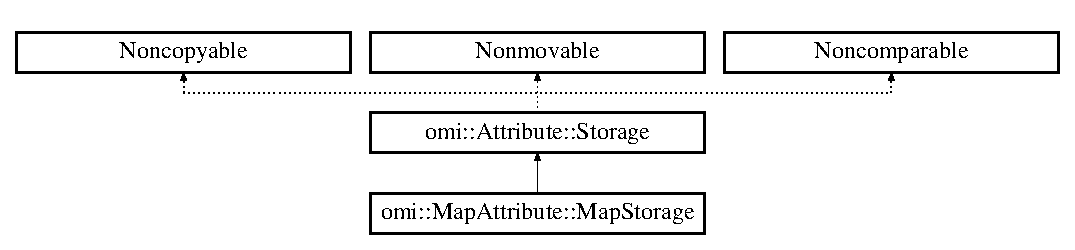
\includegraphics[height=2.916667cm]{classomi_1_1_map_attribute_1_1_map_storage}
\end{center}
\end{figure}
\subsection*{Public Member Functions}
\begin{DoxyCompactItemize}
\item 
{\footnotesize template$<$typename T\+\_\+\+Input\+Iterator $>$ }\\{\bfseries Map\+Storage} (const T\+\_\+\+Input\+Iterator \&first, const T\+\_\+\+Input\+Iterator \&last)\hypertarget{classomi_1_1_map_attribute_1_1_map_storage_a6b0be9f731a857df18a44345eb8142cf}{}\label{classomi_1_1_map_attribute_1_1_map_storage_a6b0be9f731a857df18a44345eb8142cf}

\item 
virtual O\+M\+I\+\_\+\+A\+P\+I\+\_\+\+G\+L\+O\+B\+AL bool \hyperlink{classomi_1_1_map_attribute_1_1_map_storage_ace7c69c5dcdbecaa137529cd6de221d1}{equals} (const \hyperlink{classomi_1_1_attribute_1_1_storage}{Storage} $\ast$other)\hypertarget{classomi_1_1_map_attribute_1_1_map_storage_ace7c69c5dcdbecaa137529cd6de221d1}{}\label{classomi_1_1_map_attribute_1_1_map_storage_ace7c69c5dcdbecaa137529cd6de221d1}

\begin{DoxyCompactList}\small\item\em Compares whether this storage has equality with the other given storage pointer. \end{DoxyCompactList}\item 
virtual O\+M\+I\+\_\+\+A\+P\+I\+\_\+\+G\+L\+O\+B\+AL \hyperlink{classomi_1_1_attribute_1_1_storage}{Storage} $\ast$ {\bfseries copy\+\_\+for\+\_\+overwrite} (bool soft)\hypertarget{classomi_1_1_map_attribute_1_1_map_storage_ad85c170a81a3b719ff43caf33193e64c}{}\label{classomi_1_1_map_attribute_1_1_map_storage_ad85c170a81a3b719ff43caf33193e64c}

\item 
virtual O\+M\+I\+\_\+\+A\+P\+I\+\_\+\+G\+L\+O\+B\+AL void {\bfseries string\+\_\+repr} (std\+::size\+\_\+t indentation, arc\+::str\+::\+U\+T\+F8\+String \&s) const \hypertarget{classomi_1_1_map_attribute_1_1_map_storage_aaa38c91f875226c3e49c6310910e7531}{}\label{classomi_1_1_map_attribute_1_1_map_storage_aaa38c91f875226c3e49c6310910e7531}

\end{DoxyCompactItemize}
\subsection*{Public Attributes}
\begin{DoxyCompactItemize}
\item 
\hyperlink{classomi_1_1_map_attribute_ac5a11b90e684944a18bcd18376d7eed1}{Data\+Type} {\bfseries m\+\_\+data}\hypertarget{classomi_1_1_map_attribute_1_1_map_storage_acbd10ad38a02c772b4e1dc00656cd145}{}\label{classomi_1_1_map_attribute_1_1_map_storage_acbd10ad38a02c772b4e1dc00656cd145}

\end{DoxyCompactItemize}


The documentation for this class was generated from the following file\+:\begin{DoxyCompactItemize}
\item 
/home/david/\+Dropbox/\+Development/\+Omicron/\+Omicron/src/cpp/omicron/api/common/attribute/\hyperlink{_map_attribute_8hpp}{Map\+Attribute.\+hpp}\end{DoxyCompactItemize}

\hypertarget{classomi_1_1asset_1_1_material}{}\section{omi\+:\+:asset\+:\+:Material Class Reference}
\label{classomi_1_1asset_1_1_material}\index{omi\+::asset\+::\+Material@{omi\+::asset\+::\+Material}}
Inheritance diagram for omi\+:\+:asset\+:\+:Material\+:\begin{figure}[H]
\begin{center}
\leavevmode
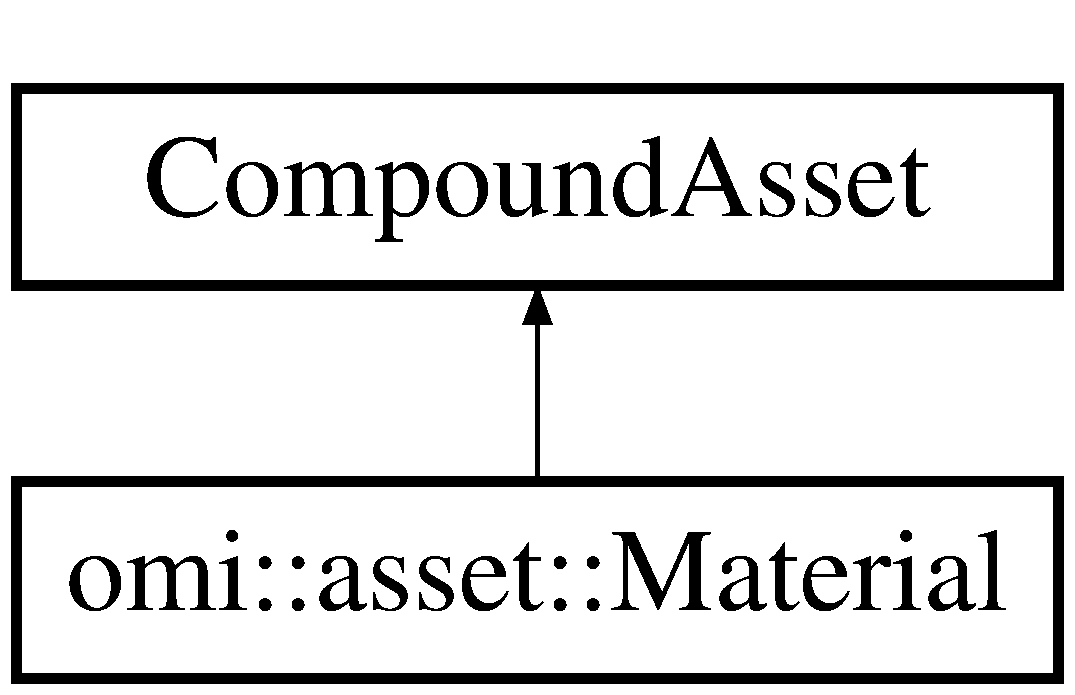
\includegraphics[height=2.000000cm]{classomi_1_1asset_1_1_material}
\end{center}
\end{figure}


The documentation for this class was generated from the following file\+:\begin{DoxyCompactItemize}
\item 
/home/david/\+Dropbox/\+Development/\+Omicron/\+Omicron/src/cpp/omicron/api/asset/types/bk/\hyperlink{_material_asset_8hpp}{Material\+Asset.\+hpp}\end{DoxyCompactItemize}

\hypertarget{classomi_1_1xform_1_1_matrix}{}\section{omi\+:\+:xform\+:\+:Matrix Class Reference}
\label{classomi_1_1xform_1_1_matrix}\index{omi\+::xform\+::\+Matrix@{omi\+::xform\+::\+Matrix}}


T\+O\+DO\+:  




{\ttfamily \#include $<$Matrix.\+hpp$>$}

Inheritance diagram for omi\+:\+:xform\+:\+:Matrix\+:\begin{figure}[H]
\begin{center}
\leavevmode
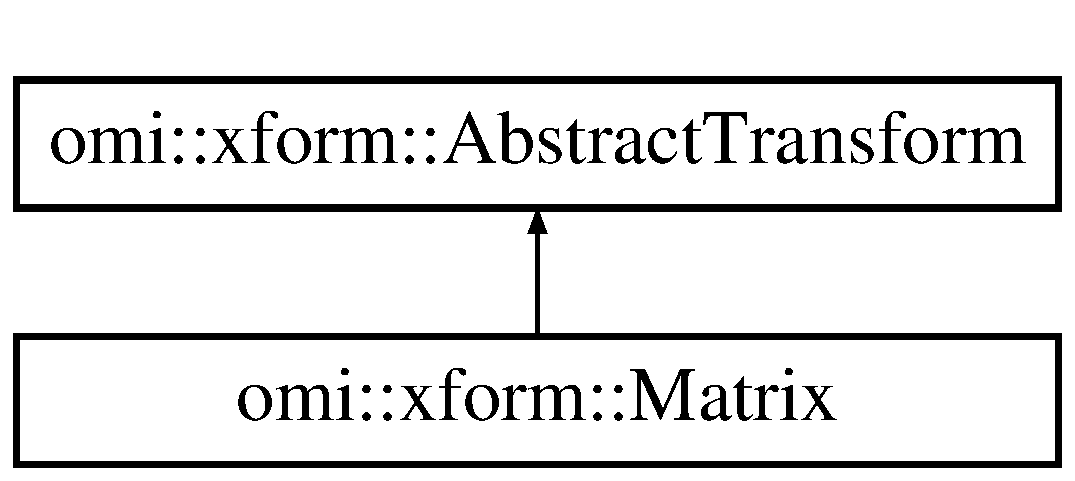
\includegraphics[height=2.000000cm]{classomi_1_1xform_1_1_matrix}
\end{center}
\end{figure}


\subsection{Detailed Description}
T\+O\+DO\+: 

The documentation for this class was generated from the following file\+:\begin{DoxyCompactItemize}
\item 
/home/david/\+Dropbox/\+Development/\+Omicron/\+Omicron/src/cpp/omicron/api/xform/\hyperlink{_matrix_8hpp}{Matrix.\+hpp}\end{DoxyCompactItemize}

\hypertarget{classomi_1_1asset_1_1_mesh}{}\section{omi\+:\+:asset\+:\+:Mesh Class Reference}
\label{classomi_1_1asset_1_1_mesh}\index{omi\+::asset\+::\+Mesh@{omi\+::asset\+::\+Mesh}}
Inheritance diagram for omi\+:\+:asset\+:\+:Mesh\+:\begin{figure}[H]
\begin{center}
\leavevmode
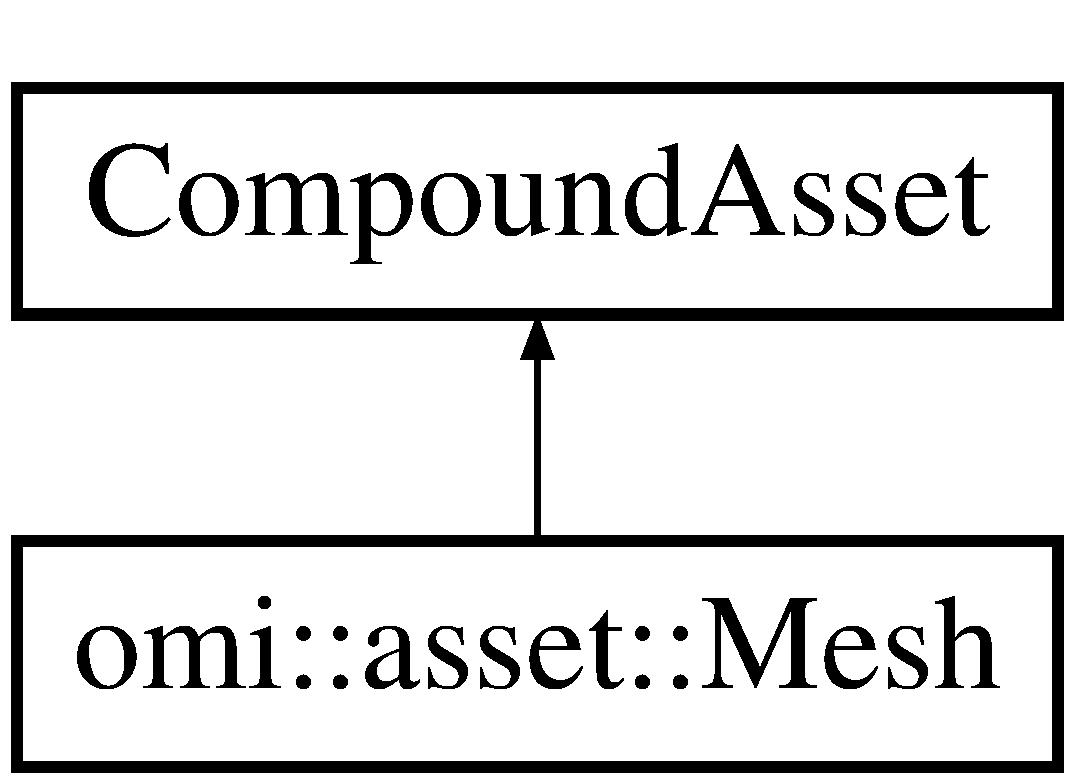
\includegraphics[height=2.000000cm]{classomi_1_1asset_1_1_mesh}
\end{center}
\end{figure}


The documentation for this class was generated from the following file\+:\begin{DoxyCompactItemize}
\item 
/home/david/\+Dropbox/\+Development/\+Omicron/\+Omicron/src/cpp/omicron/api/asset/types/bk/\hyperlink{_mesh_asset_8hpp}{Mesh\+Asset.\+hpp}\end{DoxyCompactItemize}

\hypertarget{classomi_1_1asset_1_1_o_b_j_resource}{}\section{omi\+:\+:asset\+:\+:O\+B\+J\+Resource Class Reference}
\label{classomi_1_1asset_1_1_o_b_j_resource}\index{omi\+::asset\+::\+O\+B\+J\+Resource@{omi\+::asset\+::\+O\+B\+J\+Resource}}
Inheritance diagram for omi\+:\+:asset\+:\+:O\+B\+J\+Resource\+:\begin{figure}[H]
\begin{center}
\leavevmode
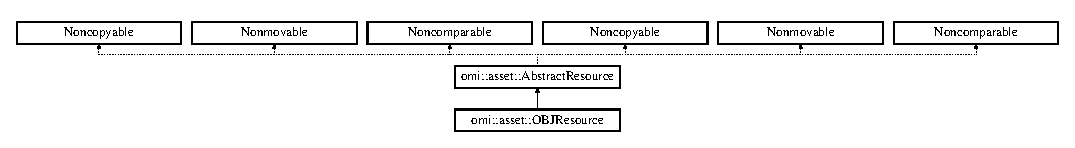
\includegraphics[height=1.546961cm]{classomi_1_1asset_1_1_o_b_j_resource}
\end{center}
\end{figure}
\subsection*{Public Member Functions}
\begin{DoxyCompactItemize}
\item 
virtual O\+M\+I\+\_\+\+A\+P\+I\+\_\+\+G\+L\+O\+B\+AL void {\bfseries load} (arc\+::io\+::sys\+::\+File\+Reader $\ast$reader)\hypertarget{classomi_1_1asset_1_1_o_b_j_resource_a6cb28146fb0875b59dc19d937a48c34b}{}\label{classomi_1_1asset_1_1_o_b_j_resource_a6cb28146fb0875b59dc19d937a48c34b}

\item 
virtual O\+M\+I\+\_\+\+A\+P\+I\+\_\+\+G\+L\+O\+B\+AL void {\bfseries release} ()\hypertarget{classomi_1_1asset_1_1_o_b_j_resource_a90b2328900d521d302d7a355655cafff}{}\label{classomi_1_1asset_1_1_o_b_j_resource_a90b2328900d521d302d7a355655cafff}

\end{DoxyCompactItemize}


The documentation for this class was generated from the following file\+:\begin{DoxyCompactItemize}
\item 
/home/david/\+Dropbox/\+Development/\+Omicron/\+Omicron/src/cpp/omicron/api/asset/resource/\hyperlink{_o_b_j_resource_8hpp}{O\+B\+J\+Resource.\+hpp}\end{DoxyCompactItemize}

\hypertarget{classomi_1_1ss_1_1_physics}{}\section{omi\+:\+:ss\+:\+:Physics Class Reference}
\label{classomi_1_1ss_1_1_physics}\index{omi\+::ss\+::\+Physics@{omi\+::ss\+::\+Physics}}


T\+O\+DO\+:  




{\ttfamily \#include $<$Physics.\+hpp$>$}

Inheritance diagram for omi\+:\+:ss\+:\+:Physics\+:\begin{figure}[H]
\begin{center}
\leavevmode
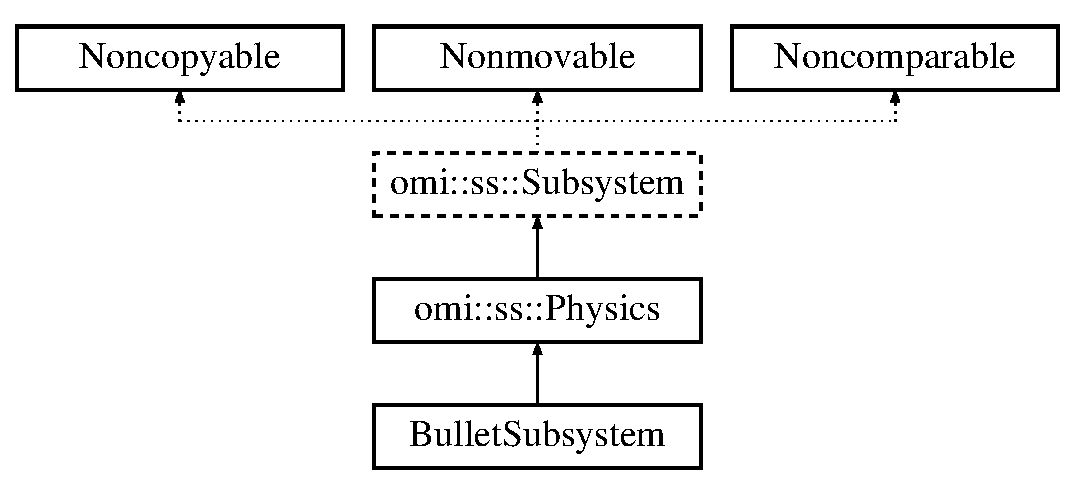
\includegraphics[height=4.000000cm]{classomi_1_1ss_1_1_physics}
\end{center}
\end{figure}
\subsection*{Public Member Functions}
\begin{DoxyCompactItemize}
\item 
\hyperlink{classomi_1_1ss_1_1_physics_a7988787f455310cfa87ce29869bde107}{Physics} ()\hypertarget{classomi_1_1ss_1_1_physics_a7988787f455310cfa87ce29869bde107}{}\label{classomi_1_1ss_1_1_physics_a7988787f455310cfa87ce29869bde107}

\begin{DoxyCompactList}\small\item\em T\+O\+DO\+: \end{DoxyCompactList}\end{DoxyCompactItemize}
\subsection*{Additional Inherited Members}


\subsection{Detailed Description}
T\+O\+DO\+: 

The documentation for this class was generated from the following file\+:\begin{DoxyCompactItemize}
\item 
/home/david/\+Dropbox/\+Development/\+Omicron/\+Omicron/src/cpp/omicron/subsystem/\hyperlink{_physics_8hpp}{Physics.\+hpp}\end{DoxyCompactItemize}

\hypertarget{class_p_x_subsystem}{}\section{P\+X\+Subsystem Class Reference}
\label{class_p_x_subsystem}\index{P\+X\+Subsystem@{P\+X\+Subsystem}}


T\+O\+DO.  




{\ttfamily \#include $<$P\+X\+Subsystem.\+hpp$>$}

Inheritance diagram for P\+X\+Subsystem\+:\begin{figure}[H]
\begin{center}
\leavevmode
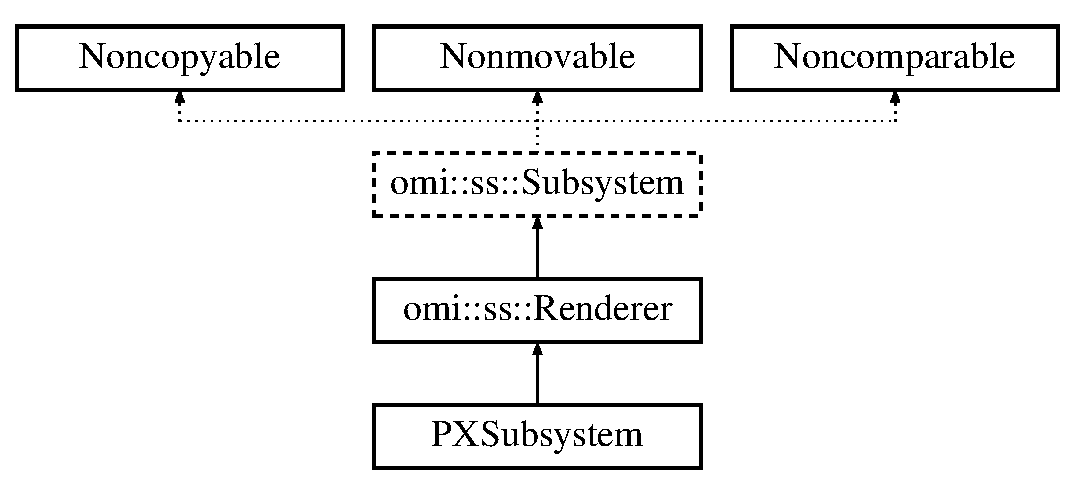
\includegraphics[height=4.000000cm]{class_p_x_subsystem}
\end{center}
\end{figure}
\subsection*{Public Member Functions}
\begin{DoxyCompactItemize}
\item 
virtual void \hyperlink{class_p_x_subsystem_a8c051bb5e7277c6754647a53885b6348}{startup} ()
\begin{DoxyCompactList}\small\item\em Startups up this subsystem. \end{DoxyCompactList}\item 
virtual void \hyperlink{class_p_x_subsystem_adabd11441f7c81b81aba456f6d825279}{shutdown} ()
\begin{DoxyCompactList}\small\item\em Performs shutdown of this subsystem. \end{DoxyCompactList}\item 
virtual void \hyperlink{class_p_x_subsystem_ae2dba562627b2cc26cbc880942fc5a9b}{setup\+\_\+rendering} ()\hypertarget{class_p_x_subsystem_ae2dba562627b2cc26cbc880942fc5a9b}{}\label{class_p_x_subsystem_ae2dba562627b2cc26cbc880942fc5a9b}

\begin{DoxyCompactList}\small\item\em Is called once a valid GL context has been established to setup rendering. \end{DoxyCompactList}\item 
virtual void \hyperlink{class_p_x_subsystem_af83fe51fbfbabd65a3d261bd62bfbfb9}{render} ()\hypertarget{class_p_x_subsystem_af83fe51fbfbabd65a3d261bd62bfbfb9}{}\label{class_p_x_subsystem_af83fe51fbfbabd65a3d261bd62bfbfb9}

\begin{DoxyCompactList}\small\item\em Is called to render the current frame. \end{DoxyCompactList}\end{DoxyCompactItemize}
\subsection*{Additional Inherited Members}


\subsection{Detailed Description}
T\+O\+DO. 

\subsection{Member Function Documentation}
\index{P\+X\+Subsystem@{P\+X\+Subsystem}!startup@{startup}}
\index{startup@{startup}!P\+X\+Subsystem@{P\+X\+Subsystem}}
\subsubsection[{\texorpdfstring{startup()}{startup()}}]{\setlength{\rightskip}{0pt plus 5cm}virtual void P\+X\+Subsystem\+::startup (
\begin{DoxyParamCaption}
{}
\end{DoxyParamCaption}
)\hspace{0.3cm}{\ttfamily [virtual]}}\hypertarget{class_p_x_subsystem_a8c051bb5e7277c6754647a53885b6348}{}\label{class_p_x_subsystem_a8c051bb5e7277c6754647a53885b6348}


Startups up this subsystem. 

\begin{DoxyWarning}{Warning}
This function should not be called manually.
\end{DoxyWarning}
Other than the constructor, this will be the first call made to this object, and will only be called once. 

Reimplemented from \hyperlink{classomi_1_1ss_1_1_subsystem_a4b0ea0b6a120c551d73151f0e0432197}{omi\+::ss\+::\+Subsystem}.

\index{P\+X\+Subsystem@{P\+X\+Subsystem}!shutdown@{shutdown}}
\index{shutdown@{shutdown}!P\+X\+Subsystem@{P\+X\+Subsystem}}
\subsubsection[{\texorpdfstring{shutdown()}{shutdown()}}]{\setlength{\rightskip}{0pt plus 5cm}virtual void P\+X\+Subsystem\+::shutdown (
\begin{DoxyParamCaption}
{}
\end{DoxyParamCaption}
)\hspace{0.3cm}{\ttfamily [virtual]}}\hypertarget{class_p_x_subsystem_adabd11441f7c81b81aba456f6d825279}{}\label{class_p_x_subsystem_adabd11441f7c81b81aba456f6d825279}


Performs shutdown of this subsystem. 

\begin{DoxyWarning}{Warning}
This function should not be called manually.
\end{DoxyWarning}
Other than the destructor, once this function has been called, no further calls to this object will be made, and shutdown will only be called once. 

Reimplemented from \hyperlink{classomi_1_1ss_1_1_subsystem_ab5855f3a5a4ec4375d2f2fea1a9bfbc5}{omi\+::ss\+::\+Subsystem}.



The documentation for this class was generated from the following file\+:\begin{DoxyCompactItemize}
\item 
/home/david/\+Dropbox/\+Development/\+Omicron/\+Omicron/src/cpp/builtin\+\_\+subsystems/pxtrace/\hyperlink{_p_x_subsystem_8hpp}{P\+X\+Subsystem.\+hpp}\end{DoxyCompactItemize}

\hypertarget{classomi__qt_1_1_qt_bootstrap}{}\section{omi\+\_\+qt\+:\+:Qt\+Bootstrap Class Reference}
\label{classomi__qt_1_1_qt_bootstrap}\index{omi\+\_\+qt\+::\+Qt\+Bootstrap@{omi\+\_\+qt\+::\+Qt\+Bootstrap}}


Handles startup and shutdown of the Omicron Qt window subsystem.  




{\ttfamily \#include $<$Qt\+Bootstrap.\+hpp$>$}

Inheritance diagram for omi\+\_\+qt\+:\+:Qt\+Bootstrap\+:\begin{figure}[H]
\begin{center}
\leavevmode
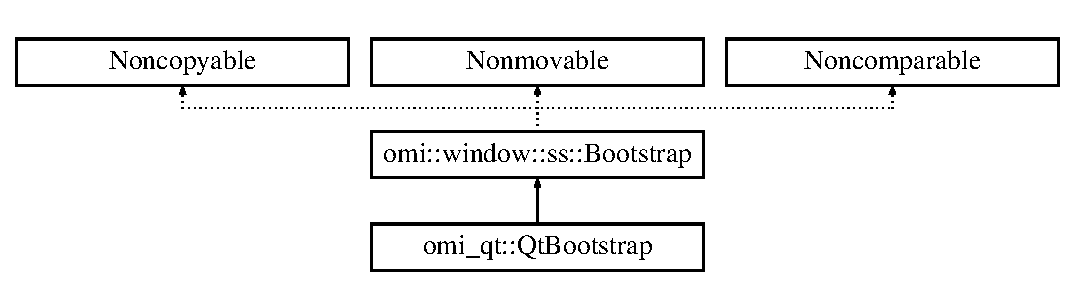
\includegraphics[height=3.000000cm]{classomi__qt_1_1_qt_bootstrap}
\end{center}
\end{figure}
\subsection*{Public Member Functions}
\begin{DoxyCompactItemize}
\item 
virtual void \hyperlink{classomi__qt_1_1_qt_bootstrap_ae86dd5217529263238e51228c248e74f}{startup} ()
\begin{DoxyCompactList}\small\item\em Starts up this Omicron window subsystem. \end{DoxyCompactList}\item 
virtual void \hyperlink{classomi__qt_1_1_qt_bootstrap_a80d703cd4cb032ed900c1d77ea0056ab}{shutdown} ()
\begin{DoxyCompactList}\small\item\em Starts up this Omicron window subsystem. \end{DoxyCompactList}\item 
virtual void \hyperlink{classomi__qt_1_1_qt_bootstrap_ab603ff5f3f6a7637b7daf143943f5e62}{start\+\_\+main\+\_\+loop} (\hyperlink{namespaceomi_1_1window_1_1ss_af42d2464a170bdfd876a35b9fde16137}{omi\+::window\+::ss\+::\+Engine\+Cycle\+Func} $\ast$engine\+\_\+cycle\+\_\+func)\hypertarget{classomi__qt_1_1_qt_bootstrap_ab603ff5f3f6a7637b7daf143943f5e62}{}\label{classomi__qt_1_1_qt_bootstrap_ab603ff5f3f6a7637b7daf143943f5e62}

\begin{DoxyCompactList}\small\item\em Starts the main loop of Omicron which will be managed by window subsystem and will call the given function every cycle of the main loop. \end{DoxyCompactList}\end{DoxyCompactItemize}
\subsection*{Static Public Member Functions}
\begin{DoxyCompactItemize}
\item 
static \hyperlink{classomi__qt_1_1_qt_bootstrap}{Qt\+Bootstrap} $\ast$ \hyperlink{classomi__qt_1_1_qt_bootstrap_a01e67a2999547d5c123a6d9296aa5e95}{get\+\_\+instance} ()\hypertarget{classomi__qt_1_1_qt_bootstrap_a01e67a2999547d5c123a6d9296aa5e95}{}\label{classomi__qt_1_1_qt_bootstrap_a01e67a2999547d5c123a6d9296aa5e95}

\begin{DoxyCompactList}\small\item\em Returns the singleton instance of the Omicron Qt bootstrapper. \end{DoxyCompactList}\end{DoxyCompactItemize}
\subsection*{Additional Inherited Members}


\subsection{Detailed Description}
Handles startup and shutdown of the Omicron Qt window subsystem. 

\subsection{Member Function Documentation}
\index{omi\+\_\+qt\+::\+Qt\+Bootstrap@{omi\+\_\+qt\+::\+Qt\+Bootstrap}!startup@{startup}}
\index{startup@{startup}!omi\+\_\+qt\+::\+Qt\+Bootstrap@{omi\+\_\+qt\+::\+Qt\+Bootstrap}}
\subsubsection[{\texorpdfstring{startup()}{startup()}}]{\setlength{\rightskip}{0pt plus 5cm}virtual void omi\+\_\+qt\+::\+Qt\+Bootstrap\+::startup (
\begin{DoxyParamCaption}
{}
\end{DoxyParamCaption}
)\hspace{0.3cm}{\ttfamily [virtual]}}\hypertarget{classomi__qt_1_1_qt_bootstrap_ae86dd5217529263238e51228c248e74f}{}\label{classomi__qt_1_1_qt_bootstrap_ae86dd5217529263238e51228c248e74f}


Starts up this Omicron window subsystem. 

Other than the Bootstrap\textquotesingle{}s constructor this will be the first call made to this object, and will only be made once. 

Reimplemented from \hyperlink{classomi_1_1window_1_1ss_1_1_bootstrap_a69b71f75e8be1496de09b3c5c647ded2}{omi\+::window\+::ss\+::\+Bootstrap}.

\index{omi\+\_\+qt\+::\+Qt\+Bootstrap@{omi\+\_\+qt\+::\+Qt\+Bootstrap}!shutdown@{shutdown}}
\index{shutdown@{shutdown}!omi\+\_\+qt\+::\+Qt\+Bootstrap@{omi\+\_\+qt\+::\+Qt\+Bootstrap}}
\subsubsection[{\texorpdfstring{shutdown()}{shutdown()}}]{\setlength{\rightskip}{0pt plus 5cm}virtual void omi\+\_\+qt\+::\+Qt\+Bootstrap\+::shutdown (
\begin{DoxyParamCaption}
{}
\end{DoxyParamCaption}
)\hspace{0.3cm}{\ttfamily [virtual]}}\hypertarget{classomi__qt_1_1_qt_bootstrap_a80d703cd4cb032ed900c1d77ea0056ab}{}\label{classomi__qt_1_1_qt_bootstrap_a80d703cd4cb032ed900c1d77ea0056ab}


Starts up this Omicron window subsystem. 

Other than the Bootstrap\textquotesingle{}s destructor this will be the last call made to this object, and will only be made once. 

Reimplemented from \hyperlink{classomi_1_1window_1_1ss_1_1_bootstrap_a6e1b4cae0710d47c28de0cda82ef9378}{omi\+::window\+::ss\+::\+Bootstrap}.



The documentation for this class was generated from the following file\+:\begin{DoxyCompactItemize}
\item 
/home/david/\+Dropbox/\+Development/\+Omicron/\+Omicron/src/cpp/builtin\+\_\+subsystems/omi\+\_\+qt/\hyperlink{_qt_bootstrap_8hpp}{Qt\+Bootstrap.\+hpp}\end{DoxyCompactItemize}

\hypertarget{classomi__qt_1_1_qt_main_window}{}\section{omi\+\_\+qt\+:\+:Qt\+Main\+Window Class Reference}
\label{classomi__qt_1_1_qt_main_window}\index{omi\+\_\+qt\+::\+Qt\+Main\+Window@{omi\+\_\+qt\+::\+Qt\+Main\+Window}}


The Qt implementation of Omicron\textquotesingle{}s main window.  




{\ttfamily \#include $<$Qt\+Main\+Window.\+hpp$>$}

Inheritance diagram for omi\+\_\+qt\+:\+:Qt\+Main\+Window\+:\begin{figure}[H]
\begin{center}
\leavevmode
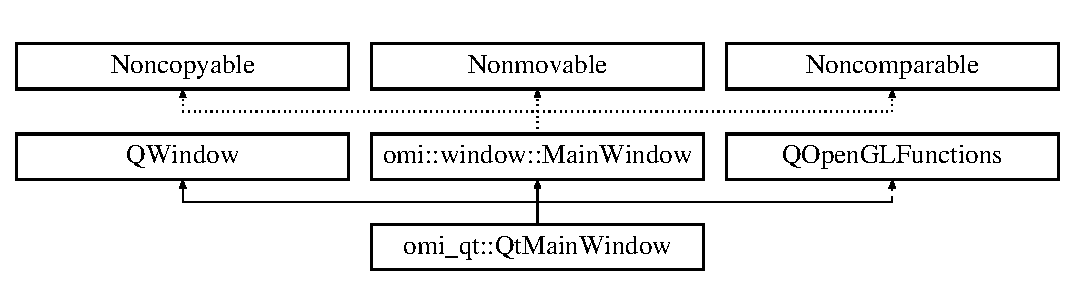
\includegraphics[height=3.000000cm]{classomi__qt_1_1_qt_main_window}
\end{center}
\end{figure}
\subsection*{Public Slots}
\begin{DoxyCompactItemize}
\item 
void \hyperlink{classomi__qt_1_1_qt_main_window_a8380f23b2a96d0a67c1b95da03e53a9a}{render\+\_\+now} ()\hypertarget{classomi__qt_1_1_qt_main_window_a8380f23b2a96d0a67c1b95da03e53a9a}{}\label{classomi__qt_1_1_qt_main_window_a8380f23b2a96d0a67c1b95da03e53a9a}

\begin{DoxyCompactList}\small\item\em Performs a rendering and update cycle of Omicron. \end{DoxyCompactList}\item 
void \hyperlink{classomi__qt_1_1_qt_main_window_aa7df1b463c14fc344ffbe99dddcf5f65}{render\+\_\+later} ()\hypertarget{classomi__qt_1_1_qt_main_window_aa7df1b463c14fc344ffbe99dddcf5f65}{}\label{classomi__qt_1_1_qt_main_window_aa7df1b463c14fc344ffbe99dddcf5f65}

\begin{DoxyCompactList}\small\item\em Calling this function will cause render\+\_\+now to be called again on the next event cycle. \end{DoxyCompactList}\end{DoxyCompactItemize}
\subsection*{Public Member Functions}
\begin{DoxyCompactItemize}
\item 
virtual \hyperlink{namespaceomi_1_1window_a096dc3d82796b93c067bca535fc0f94e}{omi\+::window\+::\+Window\+Mode} \hyperlink{classomi__qt_1_1_qt_main_window_ad85e96d8fa71189b3fc0472d0ddadc94}{get\+\_\+mode} () const \hypertarget{classomi__qt_1_1_qt_main_window_ad85e96d8fa71189b3fc0472d0ddadc94}{}\label{classomi__qt_1_1_qt_main_window_ad85e96d8fa71189b3fc0472d0ddadc94}

\begin{DoxyCompactList}\small\item\em Returns the current windowing mode of the main window. \end{DoxyCompactList}\item 
virtual void \hyperlink{classomi__qt_1_1_qt_main_window_ae2135c6116f4e9f59bf5a8b9ff489900}{set\+\_\+mode} (\hyperlink{namespaceomi_1_1window_a096dc3d82796b93c067bca535fc0f94e}{omi\+::window\+::\+Window\+Mode} mode)\hypertarget{classomi__qt_1_1_qt_main_window_ae2135c6116f4e9f59bf5a8b9ff489900}{}\label{classomi__qt_1_1_qt_main_window_ae2135c6116f4e9f59bf5a8b9ff489900}

\begin{DoxyCompactList}\small\item\em Sets the windowing mode the main window will use. \end{DoxyCompactList}\item 
virtual void {\bfseries initialize} ()\hypertarget{classomi__qt_1_1_qt_main_window_ac0234c8d46ff7eeaff496af396aa0b07}{}\label{classomi__qt_1_1_qt_main_window_ac0234c8d46ff7eeaff496af396aa0b07}

\item 
virtual void {\bfseries render} (Q\+Painter $\ast$painter)\hypertarget{classomi__qt_1_1_qt_main_window_a8fe6ae835391157ada1dfad9f0dc6471}{}\label{classomi__qt_1_1_qt_main_window_a8fe6ae835391157ada1dfad9f0dc6471}

\item 
virtual void {\bfseries render} ()\hypertarget{classomi__qt_1_1_qt_main_window_a6eb5a5e82624efe3c2f4f4d276ecba5b}{}\label{classomi__qt_1_1_qt_main_window_a6eb5a5e82624efe3c2f4f4d276ecba5b}

\end{DoxyCompactItemize}
\subsection*{Static Public Member Functions}
\begin{DoxyCompactItemize}
\item 
static \hyperlink{classomi__qt_1_1_qt_main_window}{Qt\+Main\+Window} $\ast$ {\bfseries get\+\_\+instance} ()\hypertarget{classomi__qt_1_1_qt_main_window_a4eb9d409a548e72709caed347c75fd59}{}\label{classomi__qt_1_1_qt_main_window_a4eb9d409a548e72709caed347c75fd59}

\end{DoxyCompactItemize}
\subsection*{Protected Member Functions}
\begin{DoxyCompactItemize}
\item 
void \hyperlink{classomi__qt_1_1_qt_main_window_a810a2abc13abe07839b54d9fdafb6ec5}{set\+\_\+engine\+\_\+cycle} (\hyperlink{namespaceomi_1_1window_1_1ss_af42d2464a170bdfd876a35b9fde16137}{omi\+::window\+::ss\+::\+Engine\+Cycle\+Func} $\ast$engine\+\_\+cycle\+\_\+func)\hypertarget{classomi__qt_1_1_qt_main_window_a810a2abc13abe07839b54d9fdafb6ec5}{}\label{classomi__qt_1_1_qt_main_window_a810a2abc13abe07839b54d9fdafb6ec5}

\begin{DoxyCompactList}\small\item\em Sets the function that will be used to update a cycle of the engine. \end{DoxyCompactList}\item 
bool \hyperlink{classomi__qt_1_1_qt_main_window_a358ee23739c444018367a8e6431d7d32}{event} (Q\+Event $\ast$event) Q\+\_\+\+D\+E\+C\+L\+\_\+\+O\+V\+E\+R\+R\+I\+DE\hypertarget{classomi__qt_1_1_qt_main_window_a358ee23739c444018367a8e6431d7d32}{}\label{classomi__qt_1_1_qt_main_window_a358ee23739c444018367a8e6431d7d32}

\begin{DoxyCompactList}\small\item\em Q\+Window override. \end{DoxyCompactList}\item 
void {\bfseries expose\+Event} (Q\+Expose\+Event $\ast$\hyperlink{classomi__qt_1_1_qt_main_window_a358ee23739c444018367a8e6431d7d32}{event}) Q\+\_\+\+D\+E\+C\+L\+\_\+\+O\+V\+E\+R\+R\+I\+DE\hypertarget{classomi__qt_1_1_qt_main_window_a9c04fec74da84d899820b4bd3bb8444b}{}\label{classomi__qt_1_1_qt_main_window_a9c04fec74da84d899820b4bd3bb8444b}

\end{DoxyCompactItemize}
\subsection*{Friends}
\begin{DoxyCompactItemize}
\item 
class {\bfseries Qt\+Bootstrap}\hypertarget{classomi__qt_1_1_qt_main_window_aa2f28ab658b753d4bd0b8eb0ea289b2b}{}\label{classomi__qt_1_1_qt_main_window_aa2f28ab658b753d4bd0b8eb0ea289b2b}

\end{DoxyCompactItemize}


\subsection{Detailed Description}
The Qt implementation of Omicron\textquotesingle{}s main window. 

The documentation for this class was generated from the following file\+:\begin{DoxyCompactItemize}
\item 
/home/david/\+Dropbox/\+Development/\+Omicron/\+Omicron/src/cpp/builtin\+\_\+subsystems/omi\+\_\+qt/\hyperlink{_qt_main_window_8hpp}{Qt\+Main\+Window.\+hpp}\end{DoxyCompactItemize}

\hypertarget{classomi_1_1ss_1_1_renderer}{}\section{omi\+:\+:ss\+:\+:Renderer Class Reference}
\label{classomi_1_1ss_1_1_renderer}\index{omi\+::ss\+::\+Renderer@{omi\+::ss\+::\+Renderer}}


T\+O\+DO\+:  




{\ttfamily \#include $<$Renderer.\+hpp$>$}

Inheritance diagram for omi\+:\+:ss\+:\+:Renderer\+:\begin{figure}[H]
\begin{center}
\leavevmode
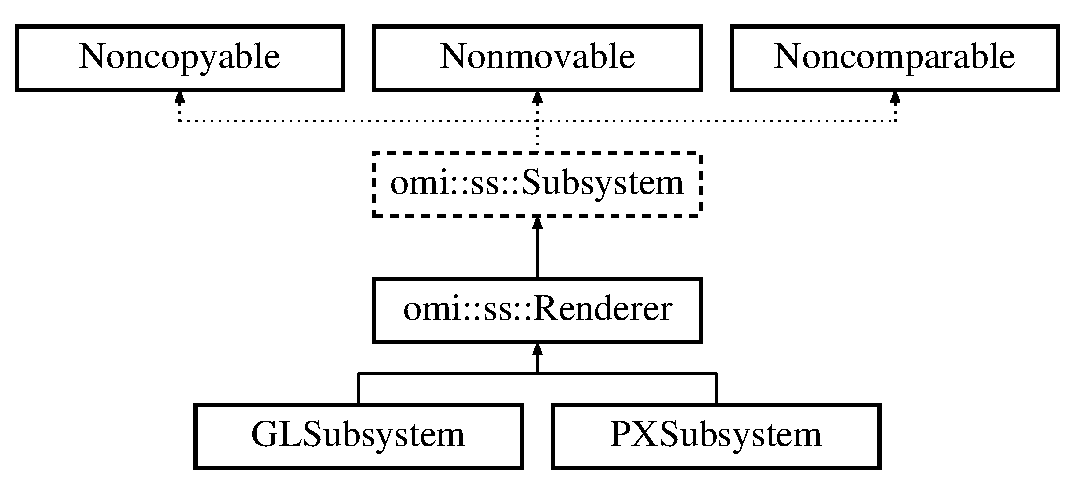
\includegraphics[height=4.000000cm]{classomi_1_1ss_1_1_renderer}
\end{center}
\end{figure}
\subsection*{Public Member Functions}
\begin{DoxyCompactItemize}
\item 
\hyperlink{classomi_1_1ss_1_1_renderer_a5cd4e0d91112f0507fa340a93f073d95}{Renderer} ()\hypertarget{classomi_1_1ss_1_1_renderer_a5cd4e0d91112f0507fa340a93f073d95}{}\label{classomi_1_1ss_1_1_renderer_a5cd4e0d91112f0507fa340a93f073d95}

\begin{DoxyCompactList}\small\item\em T\+O\+DO\+: \end{DoxyCompactList}\item 
virtual void \hyperlink{classomi_1_1ss_1_1_renderer_a5ab593d16b387b8b32c8ff315aef0abf}{setup\+\_\+rendering} ()=0\hypertarget{classomi_1_1ss_1_1_renderer_a5ab593d16b387b8b32c8ff315aef0abf}{}\label{classomi_1_1ss_1_1_renderer_a5ab593d16b387b8b32c8ff315aef0abf}

\begin{DoxyCompactList}\small\item\em Is called once a valid GL context has been established to setup rendering. \end{DoxyCompactList}\item 
virtual void \hyperlink{classomi_1_1ss_1_1_renderer_ac5a19a0f94dbcf4ac165be1fd555c3a7}{render} ()=0\hypertarget{classomi_1_1ss_1_1_renderer_ac5a19a0f94dbcf4ac165be1fd555c3a7}{}\label{classomi_1_1ss_1_1_renderer_ac5a19a0f94dbcf4ac165be1fd555c3a7}

\begin{DoxyCompactList}\small\item\em Is called to render the current frame. \end{DoxyCompactList}\end{DoxyCompactItemize}
\subsection*{Additional Inherited Members}


\subsection{Detailed Description}
T\+O\+DO\+: 

The documentation for this class was generated from the following file\+:\begin{DoxyCompactItemize}
\item 
/home/david/\+Dropbox/\+Development/\+Omicron/\+Omicron/src/cpp/omicron/subsystem/\hyperlink{_renderer_8hpp}{Renderer.\+hpp}\end{DoxyCompactItemize}

\hypertarget{classomi_1_1asset_1_1_geometry_1_1_resource}{}\section{omi\+:\+:asset\+:\+:Geometry\+:\+:Resource Class Reference}
\label{classomi_1_1asset_1_1_geometry_1_1_resource}\index{omi\+::asset\+::\+Geometry\+::\+Resource@{omi\+::asset\+::\+Geometry\+::\+Resource}}
Inheritance diagram for omi\+:\+:asset\+:\+:Geometry\+:\+:Resource\+:\begin{figure}[H]
\begin{center}
\leavevmode
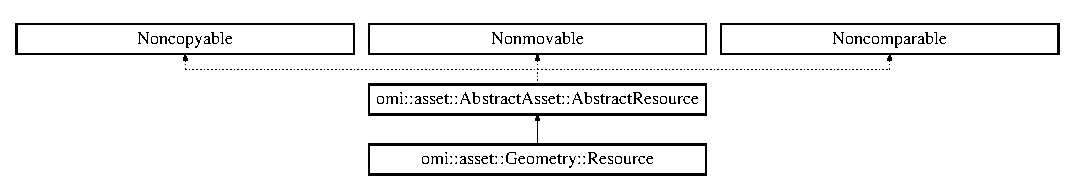
\includegraphics[height=2.113208cm]{classomi_1_1asset_1_1_geometry_1_1_resource}
\end{center}
\end{figure}


The documentation for this class was generated from the following file\+:\begin{DoxyCompactItemize}
\item 
/home/david/\+Dropbox/\+Development/\+Omicron/\+Omicron/src/cpp/omicron/api/asset/types/\hyperlink{_geometry_8hpp}{Geometry.\+hpp}\end{DoxyCompactItemize}

\hypertarget{classomi_1_1asset_1_1_shader}{}\section{omi\+:\+:asset\+:\+:Shader Class Reference}
\label{classomi_1_1asset_1_1_shader}\index{omi\+::asset\+::\+Shader@{omi\+::asset\+::\+Shader}}
Inheritance diagram for omi\+:\+:asset\+:\+:Shader\+:\begin{figure}[H]
\begin{center}
\leavevmode
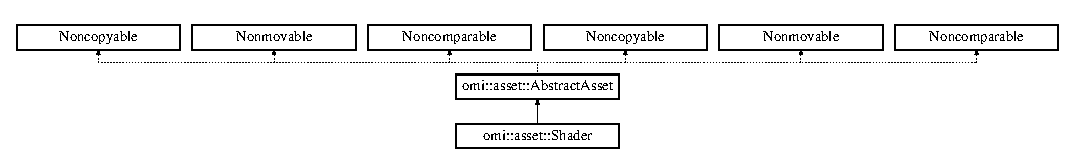
\includegraphics[height=1.772152cm]{classomi_1_1asset_1_1_shader}
\end{center}
\end{figure}


The documentation for this class was generated from the following file\+:\begin{DoxyCompactItemize}
\item 
/home/david/\+Dropbox/\+Development/\+Omicron/\+Omicron/src/cpp/omicron/api/asset/types/bk/\hyperlink{_shader_asset_8hpp}{Shader\+Asset.\+hpp}\end{DoxyCompactItemize}

\hypertarget{class_sphere}{}\section{Sphere Class Reference}
\label{class_sphere}\index{Sphere@{Sphere}}
Inheritance diagram for Sphere\+:\begin{figure}[H]
\begin{center}
\leavevmode
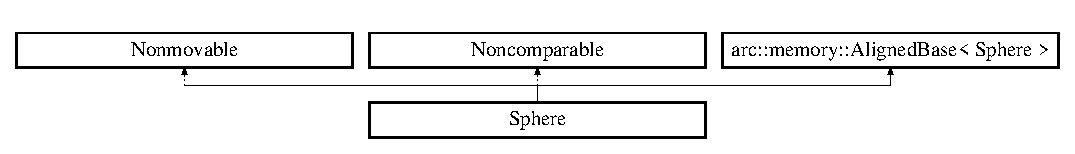
\includegraphics[height=1.616162cm]{class_sphere}
\end{center}
\end{figure}
\subsection*{Public Member Functions}
\begin{DoxyCompactItemize}
\item 
{\bfseries Sphere} (const arc\+::gm\+::\+Simd\+Vector3f \&position, float radius)\hypertarget{class_sphere_a26338c92b077ca0e576b75bb1595fab0}{}\label{class_sphere_a26338c92b077ca0e576b75bb1595fab0}

\item 
{\bfseries Sphere} (const \hyperlink{class_sphere}{Sphere} \&other)\hypertarget{class_sphere_a36f78efd8703554711ab498323d7a63f}{}\label{class_sphere_a36f78efd8703554711ab498323d7a63f}

\item 
bool {\bfseries intersects} (const arc\+::gm\+::\+Simd\+Vector3f \&ray\+\_\+origin, const arc\+::gm\+::\+Simd\+Vector3f \&ray\+\_\+direction, float \&t0, float \&t1) const \hypertarget{class_sphere_aabb55bd5e1f16f3b17f1e0509511833f}{}\label{class_sphere_aabb55bd5e1f16f3b17f1e0509511833f}

\end{DoxyCompactItemize}


The documentation for this class was generated from the following file\+:\begin{DoxyCompactItemize}
\item 
/home/david/\+Dropbox/\+Development/\+Omicron/\+Omicron/src/cpp/builtin\+\_\+subsystems/pxtrace/\hyperlink{_sphere_8hpp}{Sphere.\+hpp}\end{DoxyCompactItemize}

\hypertarget{classomi_1_1xform_1_1_s_q_t}{}\section{omi\+:\+:xform\+:\+:S\+QT Class Reference}
\label{classomi_1_1xform_1_1_s_q_t}\index{omi\+::xform\+::\+S\+QT@{omi\+::xform\+::\+S\+QT}}


T\+O\+DO\+:  




{\ttfamily \#include $<$S\+Q\+T.\+hpp$>$}

Inheritance diagram for omi\+:\+:xform\+:\+:S\+QT\+:\begin{figure}[H]
\begin{center}
\leavevmode
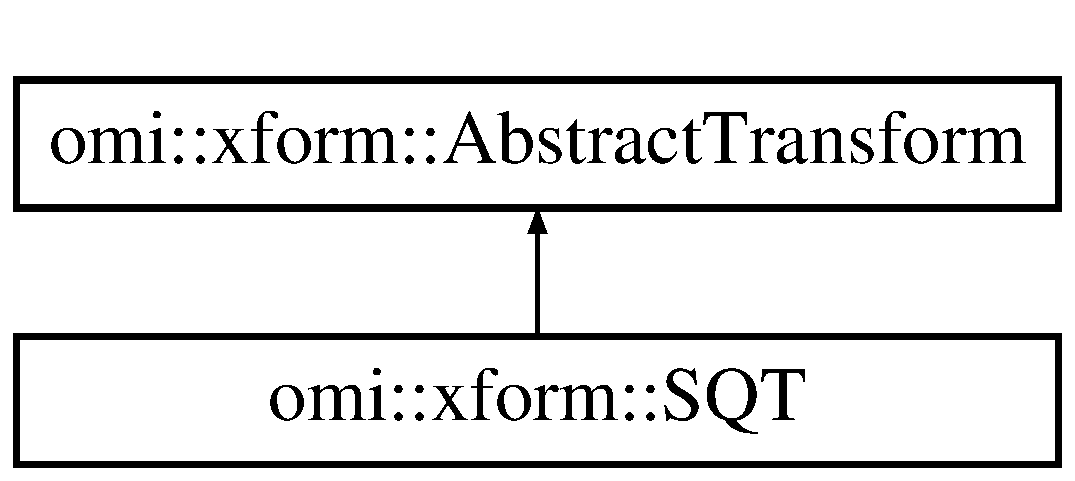
\includegraphics[height=2.000000cm]{classomi_1_1xform_1_1_s_q_t}
\end{center}
\end{figure}


\subsection{Detailed Description}
T\+O\+DO\+: 

The documentation for this class was generated from the following file\+:\begin{DoxyCompactItemize}
\item 
/home/david/\+Dropbox/\+Development/\+Omicron/\+Omicron/src/cpp/omicron/api/xform/\hyperlink{_s_q_t_8hpp}{S\+Q\+T.\+hpp}\end{DoxyCompactItemize}

\hypertarget{classomi_1_1xform_1_1_s_r_t}{}\section{omi\+:\+:xform\+:\+:S\+RT Class Reference}
\label{classomi_1_1xform_1_1_s_r_t}\index{omi\+::xform\+::\+S\+RT@{omi\+::xform\+::\+S\+RT}}


T\+O\+DO\+:  




{\ttfamily \#include $<$S\+R\+T.\+hpp$>$}

Inheritance diagram for omi\+:\+:xform\+:\+:S\+RT\+:\begin{figure}[H]
\begin{center}
\leavevmode
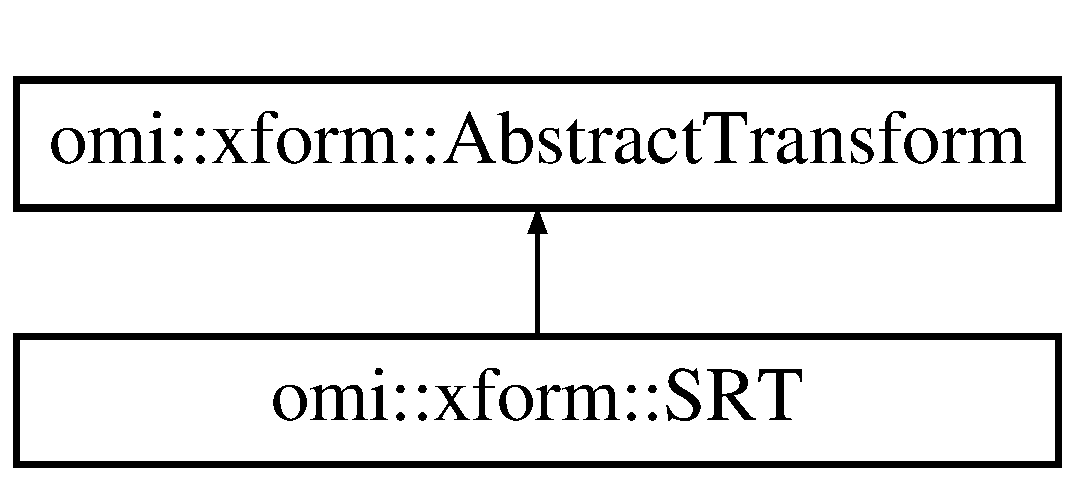
\includegraphics[height=2.000000cm]{classomi_1_1xform_1_1_s_r_t}
\end{center}
\end{figure}


\subsection{Detailed Description}
T\+O\+DO\+: 

The documentation for this class was generated from the following file\+:\begin{DoxyCompactItemize}
\item 
/home/david/\+Dropbox/\+Development/\+Omicron/\+Omicron/src/cpp/omicron/api/xform/\hyperlink{_s_r_t_8hpp}{S\+R\+T.\+hpp}\end{DoxyCompactItemize}

\hypertarget{classomi_1_1_attribute_1_1_storage}{}\section{omi\+:\+:Attribute\+:\+:Storage Class Reference}
\label{classomi_1_1_attribute_1_1_storage}\index{omi\+::\+Attribute\+::\+Storage@{omi\+::\+Attribute\+::\+Storage}}


The internal storage class defines how the contents of the attribute will be stored.  




{\ttfamily \#include $<$Attribute.\+hpp$>$}

Inheritance diagram for omi\+:\+:Attribute\+:\+:Storage\+:\begin{figure}[H]
\begin{center}
\leavevmode
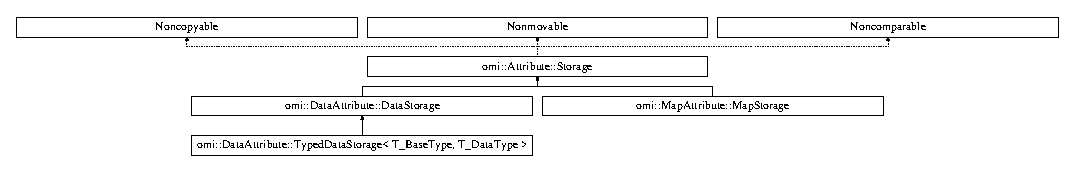
\includegraphics[height=1.866667cm]{classomi_1_1_attribute_1_1_storage}
\end{center}
\end{figure}
\subsection*{Public Member Functions}
\begin{DoxyCompactItemize}
\item 
O\+M\+I\+\_\+\+A\+P\+I\+\_\+\+G\+L\+O\+B\+AL \hyperlink{classomi_1_1_attribute_1_1_storage_a1abb81f3be684beeb8b14e92a89f81b1}{Storage} ()\hypertarget{classomi_1_1_attribute_1_1_storage_a1abb81f3be684beeb8b14e92a89f81b1}{}\label{classomi_1_1_attribute_1_1_storage_a1abb81f3be684beeb8b14e92a89f81b1}

\begin{DoxyCompactList}\small\item\em \hyperlink{classomi_1_1_attribute_1_1_storage}{Storage} super constructor. \end{DoxyCompactList}\item 
virtual bool \hyperlink{classomi_1_1_attribute_1_1_storage_aeae8905b885221ee472b741fedf233cc}{equals} (const \hyperlink{classomi_1_1_attribute_1_1_storage}{Storage} $\ast$other)=0\hypertarget{classomi_1_1_attribute_1_1_storage_aeae8905b885221ee472b741fedf233cc}{}\label{classomi_1_1_attribute_1_1_storage_aeae8905b885221ee472b741fedf233cc}

\begin{DoxyCompactList}\small\item\em Compares whether this storage has equality with the other given storage pointer. \end{DoxyCompactList}\end{DoxyCompactItemize}
\subsection*{Public Attributes}
\begin{DoxyCompactItemize}
\item 
std\+::size\+\_\+t \hyperlink{classomi_1_1_attribute_1_1_storage_a2c0290c90619a37d319085be048e8406}{m\+\_\+ref\+\_\+count}\hypertarget{classomi_1_1_attribute_1_1_storage_a2c0290c90619a37d319085be048e8406}{}\label{classomi_1_1_attribute_1_1_storage_a2c0290c90619a37d319085be048e8406}

\begin{DoxyCompactList}\small\item\em The current reference count of the storage. \end{DoxyCompactList}\item 
std\+::size\+\_\+t \hyperlink{classomi_1_1_attribute_1_1_storage_aaf58a01227aaea723df2a6ecde337090}{m\+\_\+immutable\+\_\+ref\+\_\+count}\hypertarget{classomi_1_1_attribute_1_1_storage_aaf58a01227aaea723df2a6ecde337090}{}\label{classomi_1_1_attribute_1_1_storage_aaf58a01227aaea723df2a6ecde337090}

\begin{DoxyCompactList}\small\item\em The number of immutable attributes that have references to this storage. \end{DoxyCompactList}\end{DoxyCompactItemize}


\subsection{Detailed Description}
The internal storage class defines how the contents of the attribute will be stored. 

Implementation of any sub-\/attribute types need to implement a derived storage class. 

The documentation for this class was generated from the following file\+:\begin{DoxyCompactItemize}
\item 
/home/david/\+Dropbox/\+Development/\+Omicron/\+Omicron/src/cpp/omicron/api/common/attribute/\hyperlink{_attribute_8hpp}{Attribute.\+hpp}\end{DoxyCompactItemize}

\hypertarget{classomi_1_1ss_1_1_subsystem}{}\section{omi\+:\+:ss\+:\+:Subsystem Class Reference}
\label{classomi_1_1ss_1_1_subsystem}\index{omi\+::ss\+::\+Subsystem@{omi\+::ss\+::\+Subsystem}}


T\+O\+DO\+:  




{\ttfamily \#include $<$Subsystem.\+hpp$>$}

Inheritance diagram for omi\+:\+:ss\+:\+:Subsystem\+:\begin{figure}[H]
\begin{center}
\leavevmode
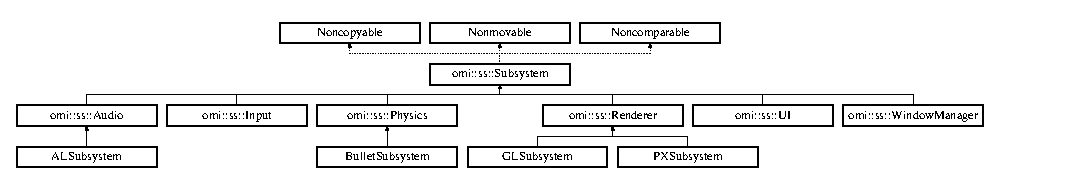
\includegraphics[height=2.025316cm]{classomi_1_1ss_1_1_subsystem}
\end{center}
\end{figure}
\subsection*{Public Types}
\begin{DoxyCompactItemize}
\item 
enum \hyperlink{classomi_1_1ss_1_1_subsystem_a4dd37e93b7d0b1b3926107258d5564f1}{Role} \{ \\*
\hyperlink{classomi_1_1ss_1_1_subsystem_a4dd37e93b7d0b1b3926107258d5564f1af9646235a1a75edc0cb539d696d6496b}{k\+Role\+Window\+Manager}, 
\hyperlink{classomi_1_1ss_1_1_subsystem_a4dd37e93b7d0b1b3926107258d5564f1ab982865b4c50613bc50b4d92216618e9}{k\+Role\+Input}, 
\hyperlink{classomi_1_1ss_1_1_subsystem_a4dd37e93b7d0b1b3926107258d5564f1a3aa5da4a253649009857e6833a9c7816}{k\+Role\+UI}, 
\hyperlink{classomi_1_1ss_1_1_subsystem_a4dd37e93b7d0b1b3926107258d5564f1aef4740e59b246203486209265f60f8c4}{k\+Role\+Renderer}, 
\\*
\hyperlink{classomi_1_1ss_1_1_subsystem_a4dd37e93b7d0b1b3926107258d5564f1adbaebaf1fcbea70c985d2343a6cd5d05}{k\+Role\+Physics}, 
\hyperlink{classomi_1_1ss_1_1_subsystem_a4dd37e93b7d0b1b3926107258d5564f1ac024816ae0332b502039a4fdbe8e38ce}{k\+Role\+Audio}
 \}\begin{DoxyCompactList}\small\item\em The possible roles a subsystem can fulfill. \end{DoxyCompactList}
\end{DoxyCompactItemize}
\subsection*{Public Member Functions}
\begin{DoxyCompactItemize}
\item 
\hyperlink{classomi_1_1ss_1_1_subsystem_aa0cef879ba17e5a5f8732dad953c431a}{Subsystem} ()\hypertarget{classomi_1_1ss_1_1_subsystem_aa0cef879ba17e5a5f8732dad953c431a}{}\label{classomi_1_1ss_1_1_subsystem_aa0cef879ba17e5a5f8732dad953c431a}

\begin{DoxyCompactList}\small\item\em T\+O\+DO. \end{DoxyCompactList}\item 
\hyperlink{classomi_1_1ss_1_1_subsystem_a4dd37e93b7d0b1b3926107258d5564f1}{Role} \hyperlink{classomi_1_1ss_1_1_subsystem_ab12658bc2095168cb0c17c3201eff894}{get\+\_\+roles} () const \hypertarget{classomi_1_1ss_1_1_subsystem_ab12658bc2095168cb0c17c3201eff894}{}\label{classomi_1_1ss_1_1_subsystem_ab12658bc2095168cb0c17c3201eff894}

\begin{DoxyCompactList}\small\item\em Returns the bit-\/field of the roles this subsystem fulfills. \end{DoxyCompactList}\item 
virtual void \hyperlink{classomi_1_1ss_1_1_subsystem_a4b0ea0b6a120c551d73151f0e0432197}{startup} ()
\begin{DoxyCompactList}\small\item\em Startups up this subsystem. \end{DoxyCompactList}\item 
virtual void \hyperlink{classomi_1_1ss_1_1_subsystem_ab5855f3a5a4ec4375d2f2fea1a9bfbc5}{shutdown} ()
\begin{DoxyCompactList}\small\item\em Performs shutdown of this subsystem. \end{DoxyCompactList}\end{DoxyCompactItemize}
\subsection*{Static Public Member Functions}
\begin{DoxyCompactItemize}
\item 
static arc\+::str\+::\+U\+T\+F8\+String \hyperlink{classomi_1_1ss_1_1_subsystem_ad928b1c2494181a422fd0e7e530a921b}{role\+\_\+to\+\_\+string} (\hyperlink{classomi_1_1ss_1_1_subsystem_a4dd37e93b7d0b1b3926107258d5564f1}{Role} role)\hypertarget{classomi_1_1ss_1_1_subsystem_ad928b1c2494181a422fd0e7e530a921b}{}\label{classomi_1_1ss_1_1_subsystem_ad928b1c2494181a422fd0e7e530a921b}

\begin{DoxyCompactList}\small\item\em Returns a string representation of the given subsystem role(s). \end{DoxyCompactList}\end{DoxyCompactItemize}
\subsection*{Protected Attributes}
\begin{DoxyCompactItemize}
\item 
\hyperlink{classomi_1_1ss_1_1_subsystem_a4dd37e93b7d0b1b3926107258d5564f1}{Role} \hyperlink{classomi_1_1ss_1_1_subsystem_ae5c24401a0352ee48f87e19c8e751c5d}{m\+\_\+roles}\hypertarget{classomi_1_1ss_1_1_subsystem_ae5c24401a0352ee48f87e19c8e751c5d}{}\label{classomi_1_1ss_1_1_subsystem_ae5c24401a0352ee48f87e19c8e751c5d}

\begin{DoxyCompactList}\small\item\em Defines the roles this \hyperlink{classomi_1_1ss_1_1_subsystem}{Subsystem} fulfills. \end{DoxyCompactList}\end{DoxyCompactItemize}


\subsection{Detailed Description}
T\+O\+DO\+: 

\subsection{Member Enumeration Documentation}
\index{omi\+::ss\+::\+Subsystem@{omi\+::ss\+::\+Subsystem}!Role@{Role}}
\index{Role@{Role}!omi\+::ss\+::\+Subsystem@{omi\+::ss\+::\+Subsystem}}
\subsubsection[{\texorpdfstring{Role}{Role}}]{\setlength{\rightskip}{0pt plus 5cm}enum {\bf omi\+::ss\+::\+Subsystem\+::\+Role}}\hypertarget{classomi_1_1ss_1_1_subsystem_a4dd37e93b7d0b1b3926107258d5564f1}{}\label{classomi_1_1ss_1_1_subsystem_a4dd37e93b7d0b1b3926107258d5564f1}


The possible roles a subsystem can fulfill. 

A subsystem may fulfill one or more of these rolls. \begin{Desc}
\item[Enumerator]\par
\begin{description}
\index{k\+Role\+Window\+Manager@{k\+Role\+Window\+Manager}!omi\+::ss\+::\+Subsystem@{omi\+::ss\+::\+Subsystem}}\index{omi\+::ss\+::\+Subsystem@{omi\+::ss\+::\+Subsystem}!k\+Role\+Window\+Manager@{k\+Role\+Window\+Manager}}\item[{\em 
k\+Role\+Window\+Manager\hypertarget{classomi_1_1ss_1_1_subsystem_a4dd37e93b7d0b1b3926107258d5564f1af9646235a1a75edc0cb539d696d6496b}{}\label{classomi_1_1ss_1_1_subsystem_a4dd37e93b7d0b1b3926107258d5564f1af9646235a1a75edc0cb539d696d6496b}
}]The subsystem will provide the window manager functionality, this includes providing the main window of Omicron, and a GL context. \index{k\+Role\+Input@{k\+Role\+Input}!omi\+::ss\+::\+Subsystem@{omi\+::ss\+::\+Subsystem}}\index{omi\+::ss\+::\+Subsystem@{omi\+::ss\+::\+Subsystem}!k\+Role\+Input@{k\+Role\+Input}}\item[{\em 
k\+Role\+Input\hypertarget{classomi_1_1ss_1_1_subsystem_a4dd37e93b7d0b1b3926107258d5564f1ab982865b4c50613bc50b4d92216618e9}{}\label{classomi_1_1ss_1_1_subsystem_a4dd37e93b7d0b1b3926107258d5564f1ab982865b4c50613bc50b4d92216618e9}
}]The subsystem will provide functionality for querying user input from one or more difference devices. \index{k\+Role\+UI@{k\+Role\+UI}!omi\+::ss\+::\+Subsystem@{omi\+::ss\+::\+Subsystem}}\index{omi\+::ss\+::\+Subsystem@{omi\+::ss\+::\+Subsystem}!k\+Role\+UI@{k\+Role\+UI}}\item[{\em 
k\+Role\+UI\hypertarget{classomi_1_1ss_1_1_subsystem_a4dd37e93b7d0b1b3926107258d5564f1a3aa5da4a253649009857e6833a9c7816}{}\label{classomi_1_1ss_1_1_subsystem_a4dd37e93b7d0b1b3926107258d5564f1a3aa5da4a253649009857e6833a9c7816}
}]The subsystem will provide \hyperlink{classomi_1_1ss_1_1_u_i}{UI} rendering and functionality. \index{k\+Role\+Renderer@{k\+Role\+Renderer}!omi\+::ss\+::\+Subsystem@{omi\+::ss\+::\+Subsystem}}\index{omi\+::ss\+::\+Subsystem@{omi\+::ss\+::\+Subsystem}!k\+Role\+Renderer@{k\+Role\+Renderer}}\item[{\em 
k\+Role\+Renderer\hypertarget{classomi_1_1ss_1_1_subsystem_a4dd37e93b7d0b1b3926107258d5564f1aef4740e59b246203486209265f60f8c4}{}\label{classomi_1_1ss_1_1_subsystem_a4dd37e93b7d0b1b3926107258d5564f1aef4740e59b246203486209265f60f8c4}
}]The subsystem will provide Omicron\textquotesingle{}s 3D rendering. \index{k\+Role\+Physics@{k\+Role\+Physics}!omi\+::ss\+::\+Subsystem@{omi\+::ss\+::\+Subsystem}}\index{omi\+::ss\+::\+Subsystem@{omi\+::ss\+::\+Subsystem}!k\+Role\+Physics@{k\+Role\+Physics}}\item[{\em 
k\+Role\+Physics\hypertarget{classomi_1_1ss_1_1_subsystem_a4dd37e93b7d0b1b3926107258d5564f1adbaebaf1fcbea70c985d2343a6cd5d05}{}\label{classomi_1_1ss_1_1_subsystem_a4dd37e93b7d0b1b3926107258d5564f1adbaebaf1fcbea70c985d2343a6cd5d05}
}]The subsystem will provide Omicron\textquotesingle{}s physics simulation systems. \index{k\+Role\+Audio@{k\+Role\+Audio}!omi\+::ss\+::\+Subsystem@{omi\+::ss\+::\+Subsystem}}\index{omi\+::ss\+::\+Subsystem@{omi\+::ss\+::\+Subsystem}!k\+Role\+Audio@{k\+Role\+Audio}}\item[{\em 
k\+Role\+Audio\hypertarget{classomi_1_1ss_1_1_subsystem_a4dd37e93b7d0b1b3926107258d5564f1ac024816ae0332b502039a4fdbe8e38ce}{}\label{classomi_1_1ss_1_1_subsystem_a4dd37e93b7d0b1b3926107258d5564f1ac024816ae0332b502039a4fdbe8e38ce}
}]The subsystem will provide audio playback. \end{description}
\end{Desc}


\subsection{Member Function Documentation}
\index{omi\+::ss\+::\+Subsystem@{omi\+::ss\+::\+Subsystem}!startup@{startup}}
\index{startup@{startup}!omi\+::ss\+::\+Subsystem@{omi\+::ss\+::\+Subsystem}}
\subsubsection[{\texorpdfstring{startup()}{startup()}}]{\setlength{\rightskip}{0pt plus 5cm}virtual void omi\+::ss\+::\+Subsystem\+::startup (
\begin{DoxyParamCaption}
{}
\end{DoxyParamCaption}
)\hspace{0.3cm}{\ttfamily [inline]}, {\ttfamily [virtual]}}\hypertarget{classomi_1_1ss_1_1_subsystem_a4b0ea0b6a120c551d73151f0e0432197}{}\label{classomi_1_1ss_1_1_subsystem_a4b0ea0b6a120c551d73151f0e0432197}


Startups up this subsystem. 

\begin{DoxyWarning}{Warning}
This function should not be called manually.
\end{DoxyWarning}
Other than the constructor, this will be the first call made to this object, and will only be called once. 

Reimplemented in \hyperlink{class_p_x_subsystem_a8c051bb5e7277c6754647a53885b6348}{P\+X\+Subsystem}, \hyperlink{class_a_l_subsystem_a46de88998ac77d7d64532471d30028b3}{A\+L\+Subsystem}, \hyperlink{class_bullet_subsystem_a3221cf461749b3b7a4a9a9784f06b5b4}{Bullet\+Subsystem}, and \hyperlink{class_g_l_subsystem_a05c8c799107f035e4effe8b55edbe16d}{G\+L\+Subsystem}.

\index{omi\+::ss\+::\+Subsystem@{omi\+::ss\+::\+Subsystem}!shutdown@{shutdown}}
\index{shutdown@{shutdown}!omi\+::ss\+::\+Subsystem@{omi\+::ss\+::\+Subsystem}}
\subsubsection[{\texorpdfstring{shutdown()}{shutdown()}}]{\setlength{\rightskip}{0pt plus 5cm}virtual void omi\+::ss\+::\+Subsystem\+::shutdown (
\begin{DoxyParamCaption}
{}
\end{DoxyParamCaption}
)\hspace{0.3cm}{\ttfamily [inline]}, {\ttfamily [virtual]}}\hypertarget{classomi_1_1ss_1_1_subsystem_ab5855f3a5a4ec4375d2f2fea1a9bfbc5}{}\label{classomi_1_1ss_1_1_subsystem_ab5855f3a5a4ec4375d2f2fea1a9bfbc5}


Performs shutdown of this subsystem. 

\begin{DoxyWarning}{Warning}
This function should not be called manually.
\end{DoxyWarning}
Other than the destructor, once this function has been called, no further calls to this object will be made, and shutdown will only be called once. 

Reimplemented in \hyperlink{class_p_x_subsystem_adabd11441f7c81b81aba456f6d825279}{P\+X\+Subsystem}.



The documentation for this class was generated from the following file\+:\begin{DoxyCompactItemize}
\item 
/home/david/\+Dropbox/\+Development/\+Omicron/\+Omicron/src/cpp/omicron/subsystem/\hyperlink{_subsystem_8hpp}{Subsystem.\+hpp}\end{DoxyCompactItemize}

\hypertarget{classomi_1_1runtime_1_1ss_1_1_subsystem_manager}{}\section{omi\+:\+:runtime\+:\+:ss\+:\+:Subsystem\+Manager Class Reference}
\label{classomi_1_1runtime_1_1ss_1_1_subsystem_manager}\index{omi\+::runtime\+::ss\+::\+Subsystem\+Manager@{omi\+::runtime\+::ss\+::\+Subsystem\+Manager}}
Inheritance diagram for omi\+:\+:runtime\+:\+:ss\+:\+:Subsystem\+Manager\+:\begin{figure}[H]
\begin{center}
\leavevmode
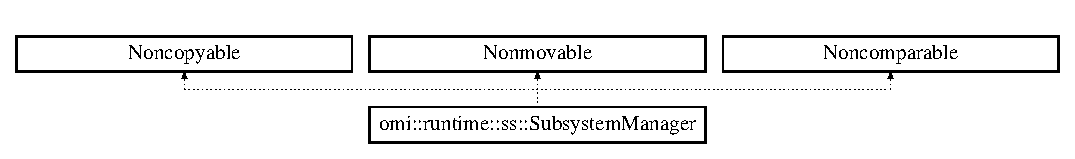
\includegraphics[height=1.689291cm]{classomi_1_1runtime_1_1ss_1_1_subsystem_manager}
\end{center}
\end{figure}
\subsection*{Public Types}
\begin{DoxyCompactItemize}
\item 
typedef std\+::vector$<$ \hyperlink{classomi_1_1ss_1_1_subsystem}{omi\+::ss\+::\+Subsystem} $\ast$ $>$ {\bfseries Subsystem\+Array}\hypertarget{classomi_1_1runtime_1_1ss_1_1_subsystem_manager_a226d578e87476b9b7ab9579d96fd9247}{}\label{classomi_1_1runtime_1_1ss_1_1_subsystem_manager_a226d578e87476b9b7ab9579d96fd9247}

\end{DoxyCompactItemize}
\subsection*{Public Member Functions}
\begin{DoxyCompactItemize}
\item 
void \hyperlink{classomi_1_1runtime_1_1ss_1_1_subsystem_manager_a18f996ef5f05428cc9cd083656dba0b9}{startup} ()
\begin{DoxyCompactList}\small\item\em Startups the manager and binds subsystem D\+S\+Os. \end{DoxyCompactList}\item 
void \hyperlink{classomi_1_1runtime_1_1ss_1_1_subsystem_manager_a9a74d6c9ecd6d5ea5fa13123f3861039}{shutdown} ()\hypertarget{classomi_1_1runtime_1_1ss_1_1_subsystem_manager_a9a74d6c9ecd6d5ea5fa13123f3861039}{}\label{classomi_1_1runtime_1_1ss_1_1_subsystem_manager_a9a74d6c9ecd6d5ea5fa13123f3861039}

\begin{DoxyCompactList}\small\item\em Shuts down the \hyperlink{classomi_1_1runtime_1_1ss_1_1_subsystem_manager}{Subsystem\+Manager}. \end{DoxyCompactList}\item 
void \hyperlink{classomi_1_1runtime_1_1ss_1_1_subsystem_manager_a61e2c524d885e5338f066424f76c0ae3}{start\+\_\+main\+\_\+loop} (\hyperlink{namespaceomi_1_1window_1_1ss_af42d2464a170bdfd876a35b9fde16137}{omi\+::window\+::ss\+::\+Engine\+Cycle\+Func} $\ast$engine\+\_\+cycle\+\_\+func)\hypertarget{classomi_1_1runtime_1_1ss_1_1_subsystem_manager_a61e2c524d885e5338f066424f76c0ae3}{}\label{classomi_1_1runtime_1_1ss_1_1_subsystem_manager_a61e2c524d885e5338f066424f76c0ae3}

\begin{DoxyCompactList}\small\item\em Starts the main loop of Omicron via the window subsystem. \end{DoxyCompactList}\end{DoxyCompactItemize}
\subsection*{Static Public Member Functions}
\begin{DoxyCompactItemize}
\item 
static \hyperlink{classomi_1_1runtime_1_1ss_1_1_subsystem_manager}{Subsystem\+Manager} $\ast$ \hyperlink{classomi_1_1runtime_1_1ss_1_1_subsystem_manager_aa676ace84e925dbebadbbb1d56ea961d}{instance} ()\hypertarget{classomi_1_1runtime_1_1ss_1_1_subsystem_manager_aa676ace84e925dbebadbbb1d56ea961d}{}\label{classomi_1_1runtime_1_1ss_1_1_subsystem_manager_aa676ace84e925dbebadbbb1d56ea961d}

\begin{DoxyCompactList}\small\item\em Returns the singleton instance of the \hyperlink{classomi_1_1runtime_1_1ss_1_1_subsystem_manager}{Subsystem\+Manager}. \end{DoxyCompactList}\end{DoxyCompactItemize}


\subsection{Member Function Documentation}
\index{omi\+::runtime\+::ss\+::\+Subsystem\+Manager@{omi\+::runtime\+::ss\+::\+Subsystem\+Manager}!startup@{startup}}
\index{startup@{startup}!omi\+::runtime\+::ss\+::\+Subsystem\+Manager@{omi\+::runtime\+::ss\+::\+Subsystem\+Manager}}
\subsubsection[{\texorpdfstring{startup()}{startup()}}]{\setlength{\rightskip}{0pt plus 5cm}void omi\+::runtime\+::ss\+::\+Subsystem\+Manager\+::startup (
\begin{DoxyParamCaption}
{}
\end{DoxyParamCaption}
)}\hypertarget{classomi_1_1runtime_1_1ss_1_1_subsystem_manager_a18f996ef5f05428cc9cd083656dba0b9}{}\label{classomi_1_1runtime_1_1ss_1_1_subsystem_manager_a18f996ef5f05428cc9cd083656dba0b9}


Startups the manager and binds subsystem D\+S\+Os. 

If the manager is already initialized this function will do nothing. 

The documentation for this class was generated from the following file\+:\begin{DoxyCompactItemize}
\item 
/home/david/\+Dropbox/\+Development/\+Omicron/\+Omicron/src/cpp/omicron/runtime/subsystem/\hyperlink{_subsystem_manager_8hpp}{Subsystem\+Manager.\+hpp}\end{DoxyCompactItemize}

\hypertarget{classomi_1_1asset_1_1_texture}{}\section{omi\+:\+:asset\+:\+:Texture Class Reference}
\label{classomi_1_1asset_1_1_texture}\index{omi\+::asset\+::\+Texture@{omi\+::asset\+::\+Texture}}
Inheritance diagram for omi\+:\+:asset\+:\+:Texture\+:\begin{figure}[H]
\begin{center}
\leavevmode
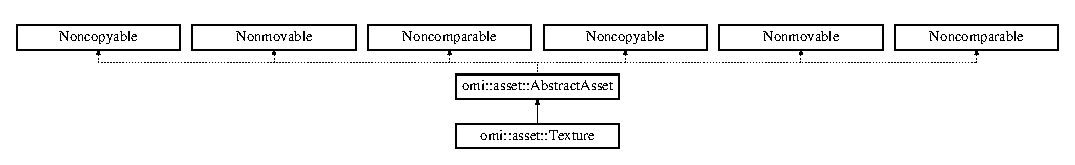
\includegraphics[height=1.772152cm]{classomi_1_1asset_1_1_texture}
\end{center}
\end{figure}


The documentation for this class was generated from the following file\+:\begin{DoxyCompactItemize}
\item 
/home/david/\+Dropbox/\+Development/\+Omicron/\+Omicron/src/cpp/omicron/api/asset/types/bk/\hyperlink{_texture_asset_8hpp}{Texture\+Asset.\+hpp}\end{DoxyCompactItemize}

\hypertarget{classomi_1_1_data_attribute_1_1_typed_data_storage}{}\section{omi\+:\+:Data\+Attribute\+:\+:Typed\+Data\+Storage$<$ T\+\_\+\+Base\+Type, T\+\_\+\+Data\+Type $>$ Class Template Reference}
\label{classomi_1_1_data_attribute_1_1_typed_data_storage}\index{omi\+::\+Data\+Attribute\+::\+Typed\+Data\+Storage$<$ T\+\_\+\+Base\+Type, T\+\_\+\+Data\+Type $>$@{omi\+::\+Data\+Attribute\+::\+Typed\+Data\+Storage$<$ T\+\_\+\+Base\+Type, T\+\_\+\+Data\+Type $>$}}
Inheritance diagram for omi\+:\+:Data\+Attribute\+:\+:Typed\+Data\+Storage$<$ T\+\_\+\+Base\+Type, T\+\_\+\+Data\+Type $>$\+:\begin{figure}[H]
\begin{center}
\leavevmode
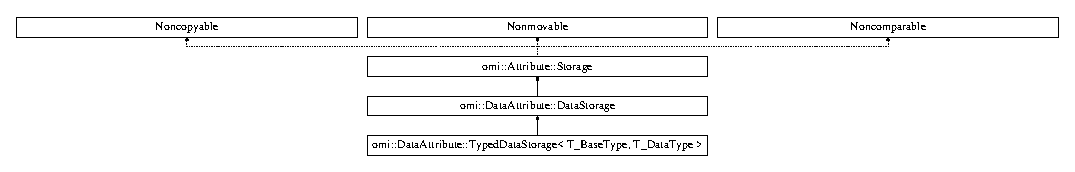
\includegraphics[height=1.866667cm]{classomi_1_1_data_attribute_1_1_typed_data_storage}
\end{center}
\end{figure}
\subsection*{Public Member Functions}
\begin{DoxyCompactItemize}
\item 
{\bfseries Typed\+Data\+Storage} (std\+::size\+\_\+t tuple\+\_\+size)\hypertarget{classomi_1_1_data_attribute_1_1_typed_data_storage_abfdd2104dc860407dc7b96ca1f9eb53c}{}\label{classomi_1_1_data_attribute_1_1_typed_data_storage_abfdd2104dc860407dc7b96ca1f9eb53c}

\item 
{\footnotesize template$<$typename T\+\_\+\+Input\+Iterator $>$ }\\{\bfseries Typed\+Data\+Storage} (const T\+\_\+\+Input\+Iterator \&first, const T\+\_\+\+Input\+Iterator \&last, std\+::size\+\_\+t tuple\+\_\+size)\hypertarget{classomi_1_1_data_attribute_1_1_typed_data_storage_a4e0a318c1b2c222b3eccff7d4fb03f09}{}\label{classomi_1_1_data_attribute_1_1_typed_data_storage_a4e0a318c1b2c222b3eccff7d4fb03f09}

\item 
virtual bool \hyperlink{classomi_1_1_data_attribute_1_1_typed_data_storage_a3116f40a9b198551f5e9107dabbda390}{equals} (const \hyperlink{classomi_1_1_attribute_1_1_storage}{Attribute\+::\+Storage} $\ast$other)\hypertarget{classomi_1_1_data_attribute_1_1_typed_data_storage_a3116f40a9b198551f5e9107dabbda390}{}\label{classomi_1_1_data_attribute_1_1_typed_data_storage_a3116f40a9b198551f5e9107dabbda390}

\begin{DoxyCompactList}\small\item\em Compares whether this storage has equality with the other given storage pointer. \end{DoxyCompactList}\item 
virtual \hyperlink{classomi_1_1_attribute_1_1_storage}{Storage} $\ast$ {\bfseries copy\+\_\+for\+\_\+overwrite} (bool soft)\hypertarget{classomi_1_1_data_attribute_1_1_typed_data_storage_a0873e417cf1fe8b250f9b67bc9a92a48}{}\label{classomi_1_1_data_attribute_1_1_typed_data_storage_a0873e417cf1fe8b250f9b67bc9a92a48}

\item 
virtual void {\bfseries string\+\_\+repr} (std\+::size\+\_\+t indentation, arc\+::str\+::\+U\+T\+F8\+String \&s) const \hypertarget{classomi_1_1_data_attribute_1_1_typed_data_storage_a7385ba2edb7164da01ca16ed4da8ef6c}{}\label{classomi_1_1_data_attribute_1_1_typed_data_storage_a7385ba2edb7164da01ca16ed4da8ef6c}

\item 
virtual std\+::size\+\_\+t {\bfseries get\+\_\+size} () const \hypertarget{classomi_1_1_data_attribute_1_1_typed_data_storage_a4252b2a48a017d16dec5b5cbe2396729}{}\label{classomi_1_1_data_attribute_1_1_typed_data_storage_a4252b2a48a017d16dec5b5cbe2396729}

\end{DoxyCompactItemize}
\subsection*{Public Attributes}
\begin{DoxyCompactItemize}
\item 
std\+::vector$<$ T\+\_\+\+Data\+Type $>$ {\bfseries m\+\_\+data}\hypertarget{classomi_1_1_data_attribute_1_1_typed_data_storage_a610f335e3d043b1ad0a12dd441ae7b34}{}\label{classomi_1_1_data_attribute_1_1_typed_data_storage_a610f335e3d043b1ad0a12dd441ae7b34}

\end{DoxyCompactItemize}


The documentation for this class was generated from the following file\+:\begin{DoxyCompactItemize}
\item 
/home/david/\+Dropbox/\+Development/\+Omicron/\+Omicron/src/cpp/omicron/api/common/attribute/\hyperlink{_data_attribute_8hpp}{Data\+Attribute.\+hpp}\end{DoxyCompactItemize}

\hypertarget{classomi_1_1ss_1_1_u_i}{}\section{omi\+:\+:ss\+:\+:UI Class Reference}
\label{classomi_1_1ss_1_1_u_i}\index{omi\+::ss\+::\+UI@{omi\+::ss\+::\+UI}}


T\+O\+DO\+:  




{\ttfamily \#include $<$U\+I.\+hpp$>$}

Inheritance diagram for omi\+:\+:ss\+:\+:UI\+:\begin{figure}[H]
\begin{center}
\leavevmode
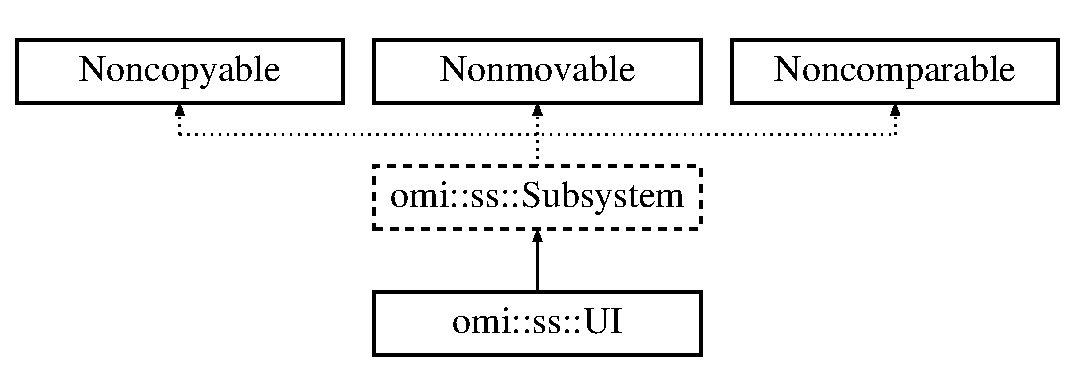
\includegraphics[height=3.000000cm]{classomi_1_1ss_1_1_u_i}
\end{center}
\end{figure}
\subsection*{Public Member Functions}
\begin{DoxyCompactItemize}
\item 
\hyperlink{classomi_1_1ss_1_1_u_i_a90c50210ffb99c79c36f9c6301861620}{UI} ()\hypertarget{classomi_1_1ss_1_1_u_i_a90c50210ffb99c79c36f9c6301861620}{}\label{classomi_1_1ss_1_1_u_i_a90c50210ffb99c79c36f9c6301861620}

\begin{DoxyCompactList}\small\item\em T\+O\+DO\+: \end{DoxyCompactList}\end{DoxyCompactItemize}
\subsection*{Additional Inherited Members}


\subsection{Detailed Description}
T\+O\+DO\+: 

The documentation for this class was generated from the following file\+:\begin{DoxyCompactItemize}
\item 
/home/david/\+Dropbox/\+Development/\+Omicron/\+Omicron/src/cpp/omicron/subsystem/\hyperlink{_u_i_8hpp}{U\+I.\+hpp}\end{DoxyCompactItemize}

\hypertarget{classomi_1_1asset_1_1_vertex_attributes}{}\section{omi\+:\+:asset\+:\+:Vertex\+Attributes Class Reference}
\label{classomi_1_1asset_1_1_vertex_attributes}\index{omi\+::asset\+::\+Vertex\+Attributes@{omi\+::asset\+::\+Vertex\+Attributes}}
Inheritance diagram for omi\+:\+:asset\+:\+:Vertex\+Attributes\+:\begin{figure}[H]
\begin{center}
\leavevmode
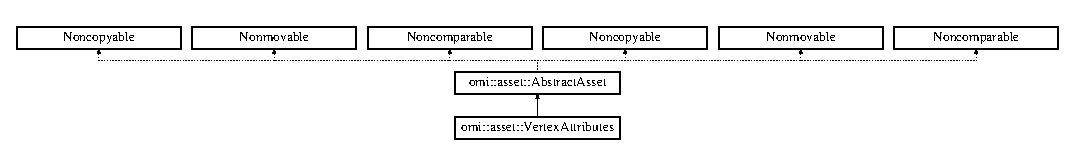
\includegraphics[height=1.647059cm]{classomi_1_1asset_1_1_vertex_attributes}
\end{center}
\end{figure}


The documentation for this class was generated from the following file\+:\begin{DoxyCompactItemize}
\item 
/home/david/\+Dropbox/\+Development/\+Omicron/\+Omicron/src/cpp/omicron/api/asset/types/bk/\hyperlink{_vertex_attributes_asset_8hpp}{Vertex\+Attributes\+Asset.\+hpp}\end{DoxyCompactItemize}

\hypertarget{classomi_1_1ss_1_1_window_manager}{}\section{omi\+:\+:ss\+:\+:Window\+Manager Class Reference}
\label{classomi_1_1ss_1_1_window_manager}\index{omi\+::ss\+::\+Window\+Manager@{omi\+::ss\+::\+Window\+Manager}}


T\+O\+DO\+:  




{\ttfamily \#include $<$Window\+Manager.\+hpp$>$}

Inheritance diagram for omi\+:\+:ss\+:\+:Window\+Manager\+:\begin{figure}[H]
\begin{center}
\leavevmode
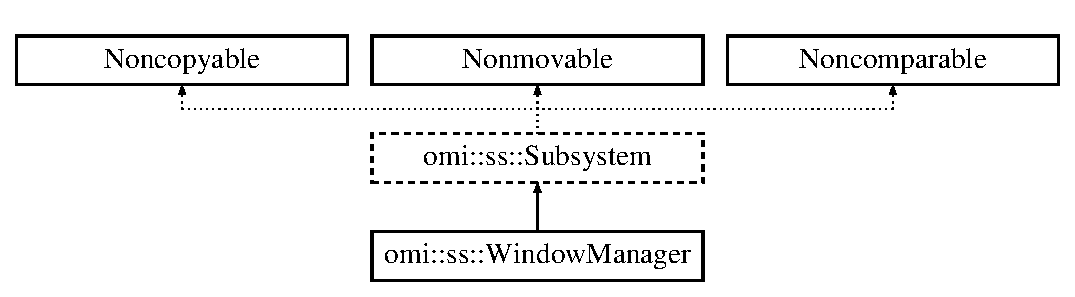
\includegraphics[height=3.000000cm]{classomi_1_1ss_1_1_window_manager}
\end{center}
\end{figure}
\subsection*{Public Types}
\begin{DoxyCompactItemize}
\item 
enum \hyperlink{classomi_1_1ss_1_1_window_manager_a84030b04e5b4c01a0d94ae67f5872cf9}{Window\+Mode} \{ \hyperlink{classomi_1_1ss_1_1_window_manager_a84030b04e5b4c01a0d94ae67f5872cf9ac5ece0f474e1fe7d5e573f193976cc7b}{k\+Mode\+Windowed}, 
\hyperlink{classomi_1_1ss_1_1_window_manager_a84030b04e5b4c01a0d94ae67f5872cf9aa4e946016788e23457b4a193e12936bb}{k\+Mode\+Borderless}, 
\hyperlink{classomi_1_1ss_1_1_window_manager_a84030b04e5b4c01a0d94ae67f5872cf9a35ada317baed6c897ffc176b37904451}{k\+Mode\+Fullscreen}
 \}\begin{DoxyCompactList}\small\item\em Defines the different modes a window can be in. \end{DoxyCompactList}
\end{DoxyCompactItemize}
\subsection*{Public Member Functions}
\begin{DoxyCompactItemize}
\item 
\hyperlink{classomi_1_1ss_1_1_window_manager_a593e6c42d7958295e36e435709d5ec06}{Window\+Manager} ()\hypertarget{classomi_1_1ss_1_1_window_manager_a593e6c42d7958295e36e435709d5ec06}{}\label{classomi_1_1ss_1_1_window_manager_a593e6c42d7958295e36e435709d5ec06}

\begin{DoxyCompactList}\small\item\em T\+O\+DO\+: \end{DoxyCompactList}\item 
virtual void \hyperlink{classomi_1_1ss_1_1_window_manager_a02b25231c0b8c035cfb4cbc962e5f7ee}{set\+\_\+mode} (\hyperlink{classomi_1_1ss_1_1_window_manager_a84030b04e5b4c01a0d94ae67f5872cf9}{Window\+Mode} mode)=0
\end{DoxyCompactItemize}
\subsection*{Additional Inherited Members}


\subsection{Detailed Description}
T\+O\+DO\+: 

\subsection{Member Enumeration Documentation}
\index{omi\+::ss\+::\+Window\+Manager@{omi\+::ss\+::\+Window\+Manager}!Window\+Mode@{Window\+Mode}}
\index{Window\+Mode@{Window\+Mode}!omi\+::ss\+::\+Window\+Manager@{omi\+::ss\+::\+Window\+Manager}}
\subsubsection[{\texorpdfstring{Window\+Mode}{WindowMode}}]{\setlength{\rightskip}{0pt plus 5cm}enum {\bf omi\+::ss\+::\+Window\+Manager\+::\+Window\+Mode}}\hypertarget{classomi_1_1ss_1_1_window_manager_a84030b04e5b4c01a0d94ae67f5872cf9}{}\label{classomi_1_1ss_1_1_window_manager_a84030b04e5b4c01a0d94ae67f5872cf9}


Defines the different modes a window can be in. 

\begin{Desc}
\item[Enumerator]\par
\begin{description}
\index{k\+Mode\+Windowed@{k\+Mode\+Windowed}!omi\+::ss\+::\+Window\+Manager@{omi\+::ss\+::\+Window\+Manager}}\index{omi\+::ss\+::\+Window\+Manager@{omi\+::ss\+::\+Window\+Manager}!k\+Mode\+Windowed@{k\+Mode\+Windowed}}\item[{\em 
k\+Mode\+Windowed\hypertarget{classomi_1_1ss_1_1_window_manager_a84030b04e5b4c01a0d94ae67f5872cf9ac5ece0f474e1fe7d5e573f193976cc7b}{}\label{classomi_1_1ss_1_1_window_manager_a84030b04e5b4c01a0d94ae67f5872cf9ac5ece0f474e1fe7d5e573f193976cc7b}
}]The window is a standard window with borders. \index{k\+Mode\+Borderless@{k\+Mode\+Borderless}!omi\+::ss\+::\+Window\+Manager@{omi\+::ss\+::\+Window\+Manager}}\index{omi\+::ss\+::\+Window\+Manager@{omi\+::ss\+::\+Window\+Manager}!k\+Mode\+Borderless@{k\+Mode\+Borderless}}\item[{\em 
k\+Mode\+Borderless\hypertarget{classomi_1_1ss_1_1_window_manager_a84030b04e5b4c01a0d94ae67f5872cf9aa4e946016788e23457b4a193e12936bb}{}\label{classomi_1_1ss_1_1_window_manager_a84030b04e5b4c01a0d94ae67f5872cf9aa4e946016788e23457b4a193e12936bb}
}]A window without standard operating system provided borders. \index{k\+Mode\+Fullscreen@{k\+Mode\+Fullscreen}!omi\+::ss\+::\+Window\+Manager@{omi\+::ss\+::\+Window\+Manager}}\index{omi\+::ss\+::\+Window\+Manager@{omi\+::ss\+::\+Window\+Manager}!k\+Mode\+Fullscreen@{k\+Mode\+Fullscreen}}\item[{\em 
k\+Mode\+Fullscreen\hypertarget{classomi_1_1ss_1_1_window_manager_a84030b04e5b4c01a0d94ae67f5872cf9a35ada317baed6c897ffc176b37904451}{}\label{classomi_1_1ss_1_1_window_manager_a84030b04e5b4c01a0d94ae67f5872cf9a35ada317baed6c897ffc176b37904451}
}]A window without borders and also occupies the entire screen. \end{description}
\end{Desc}


\subsection{Member Function Documentation}
\index{omi\+::ss\+::\+Window\+Manager@{omi\+::ss\+::\+Window\+Manager}!set\+\_\+mode@{set\+\_\+mode}}
\index{set\+\_\+mode@{set\+\_\+mode}!omi\+::ss\+::\+Window\+Manager@{omi\+::ss\+::\+Window\+Manager}}
\subsubsection[{\texorpdfstring{set\+\_\+mode(\+Window\+Mode mode)=0}{set_mode(WindowMode mode)=0}}]{\setlength{\rightskip}{0pt plus 5cm}virtual void omi\+::ss\+::\+Window\+Manager\+::set\+\_\+mode (
\begin{DoxyParamCaption}
\item[{{\bf Window\+Mode}}]{mode}
\end{DoxyParamCaption}
)\hspace{0.3cm}{\ttfamily [pure virtual]}}\hypertarget{classomi_1_1ss_1_1_window_manager_a02b25231c0b8c035cfb4cbc962e5f7ee}{}\label{classomi_1_1ss_1_1_window_manager_a02b25231c0b8c035cfb4cbc962e5f7ee}
Sets the window mode to be used. 

The documentation for this class was generated from the following file\+:\begin{DoxyCompactItemize}
\item 
/home/david/\+Dropbox/\+Development/\+Omicron/\+Omicron/src/cpp/omicron/subsystem/\hyperlink{_window_manager_8hpp}{Window\+Manager.\+hpp}\end{DoxyCompactItemize}

\hypertarget{classomi_1_1runtime_1_1ss_1_1_window_subsystem}{}\section{omi\+:\+:runtime\+:\+:ss\+:\+:Window\+Subsystem Class Reference}
\label{classomi_1_1runtime_1_1ss_1_1_window_subsystem}\index{omi\+::runtime\+::ss\+::\+Window\+Subsystem@{omi\+::runtime\+::ss\+::\+Window\+Subsystem}}


Holds the components that provide access to the bound window subsystem.  




{\ttfamily \#include $<$Window\+Subsystem.\+hpp$>$}

Inheritance diagram for omi\+:\+:runtime\+:\+:ss\+:\+:Window\+Subsystem\+:\begin{figure}[H]
\begin{center}
\leavevmode
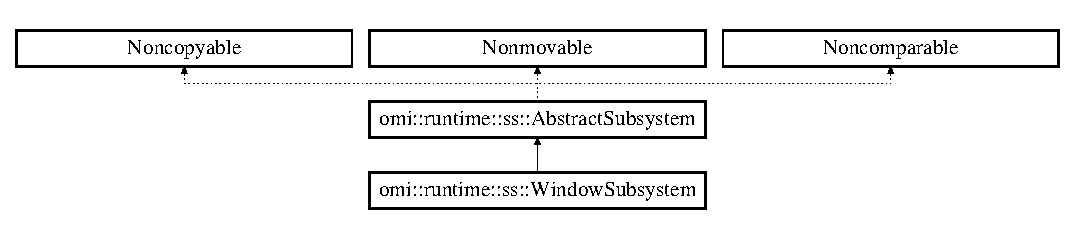
\includegraphics[height=2.580645cm]{classomi_1_1runtime_1_1ss_1_1_window_subsystem}
\end{center}
\end{figure}
\subsection*{Public Member Functions}
\begin{DoxyCompactItemize}
\item 
virtual void \hyperlink{classomi_1_1runtime_1_1ss_1_1_window_subsystem_a31c8f26f08cc6475e4155470713fb440}{bind} (arc\+::io\+::dl\+::\+Handle library)\hypertarget{classomi_1_1runtime_1_1ss_1_1_window_subsystem_a31c8f26f08cc6475e4155470713fb440}{}\label{classomi_1_1runtime_1_1ss_1_1_window_subsystem_a31c8f26f08cc6475e4155470713fb440}

\begin{DoxyCompactList}\small\item\em Loads the subsystem from the given dynamic library and binds it into Omicron. \end{DoxyCompactList}\item 
virtual void \hyperlink{classomi_1_1runtime_1_1ss_1_1_window_subsystem_aa96c852ad0db077bacaabb55603cfcd1}{startup} ()\hypertarget{classomi_1_1runtime_1_1ss_1_1_window_subsystem_aa96c852ad0db077bacaabb55603cfcd1}{}\label{classomi_1_1runtime_1_1ss_1_1_window_subsystem_aa96c852ad0db077bacaabb55603cfcd1}

\begin{DoxyCompactList}\small\item\em Starts up this subsystem. \end{DoxyCompactList}\item 
virtual void \hyperlink{classomi_1_1runtime_1_1ss_1_1_window_subsystem_a86b3dbc5b0a67e77de1ca0cfe5cecbd8}{release} ()
\begin{DoxyCompactList}\small\item\em Unbinds the subsystem from Omicron and shuts it down. \end{DoxyCompactList}\item 
void \hyperlink{classomi_1_1runtime_1_1ss_1_1_window_subsystem_a0edb4d11599ffafd6fd8d281dbeb5571}{start\+\_\+main\+\_\+loop} (\hyperlink{namespaceomi_1_1window_1_1ss_af42d2464a170bdfd876a35b9fde16137}{omi\+::window\+::ss\+::\+Engine\+Cycle\+Func} $\ast$engine\+\_\+cycle\+\_\+func)\hypertarget{classomi_1_1runtime_1_1ss_1_1_window_subsystem_a0edb4d11599ffafd6fd8d281dbeb5571}{}\label{classomi_1_1runtime_1_1ss_1_1_window_subsystem_a0edb4d11599ffafd6fd8d281dbeb5571}

\begin{DoxyCompactList}\small\item\em Starts the main loop of Omicron via the window subsystem. \end{DoxyCompactList}\end{DoxyCompactItemize}


\subsection{Detailed Description}
Holds the components that provide access to the bound window subsystem. 

\subsection{Member Function Documentation}
\index{omi\+::runtime\+::ss\+::\+Window\+Subsystem@{omi\+::runtime\+::ss\+::\+Window\+Subsystem}!release@{release}}
\index{release@{release}!omi\+::runtime\+::ss\+::\+Window\+Subsystem@{omi\+::runtime\+::ss\+::\+Window\+Subsystem}}
\subsubsection[{\texorpdfstring{release()}{release()}}]{\setlength{\rightskip}{0pt plus 5cm}virtual void omi\+::runtime\+::ss\+::\+Window\+Subsystem\+::release (
\begin{DoxyParamCaption}
{}
\end{DoxyParamCaption}
)\hspace{0.3cm}{\ttfamily [virtual]}}\hypertarget{classomi_1_1runtime_1_1ss_1_1_window_subsystem_a86b3dbc5b0a67e77de1ca0cfe5cecbd8}{}\label{classomi_1_1runtime_1_1ss_1_1_window_subsystem_a86b3dbc5b0a67e77de1ca0cfe5cecbd8}


Unbinds the subsystem from Omicron and shuts it down. 

\begin{DoxyWarning}{Warning}
This should close the dynamic library, this is done by the \hyperlink{classomi_1_1runtime_1_1ss_1_1_subsystem_manager}{Subsystem\+Manager}. 
\end{DoxyWarning}


Implements \hyperlink{classomi_1_1runtime_1_1ss_1_1_abstract_subsystem_ad5bf243e9a1b0ae94aaf3e6a998bdbf9}{omi\+::runtime\+::ss\+::\+Abstract\+Subsystem}.



The documentation for this class was generated from the following file\+:\begin{DoxyCompactItemize}
\item 
/home/david/\+Dropbox/\+Development/\+Omicron/\+Omicron/src/cpp/omicron/runtime/subsystem/\hyperlink{_window_subsystem_8hpp}{Window\+Subsystem.\+hpp}\end{DoxyCompactItemize}

\chapter{File Documentation}
\hypertarget{_a_l_subsystem_8hpp}{}\section{/home/david/\+Dropbox/\+Development/\+Omicron/\+Omicron/src/cpp/builtin\+\_\+subsystems/omi\+\_\+al/\+A\+L\+Subsystem.hpp File Reference}
\label{_a_l_subsystem_8hpp}\index{/home/david/\+Dropbox/\+Development/\+Omicron/\+Omicron/src/cpp/builtin\+\_\+subsystems/omi\+\_\+al/\+A\+L\+Subsystem.\+hpp@{/home/david/\+Dropbox/\+Development/\+Omicron/\+Omicron/src/cpp/builtin\+\_\+subsystems/omi\+\_\+al/\+A\+L\+Subsystem.\+hpp}}
{\ttfamily \#include $<$omicron/subsystem/\+Audio.\+hpp$>$}\\*
\subsection*{Classes}
\begin{DoxyCompactItemize}
\item 
class \hyperlink{class_a_l_subsystem}{A\+L\+Subsystem}
\begin{DoxyCompactList}\small\item\em T\+O\+DO. \end{DoxyCompactList}\end{DoxyCompactItemize}


\subsection{Detailed Description}
\begin{DoxyAuthor}{Author}
David Saxon 
\end{DoxyAuthor}

\hypertarget{_bullet_subsystem_8hpp}{}\section{/home/david/\+Dropbox/\+Development/\+Omicron/\+Omicron/src/cpp/builtin\+\_\+subsystems/omi\+\_\+bullet/\+Bullet\+Subsystem.hpp File Reference}
\label{_bullet_subsystem_8hpp}\index{/home/david/\+Dropbox/\+Development/\+Omicron/\+Omicron/src/cpp/builtin\+\_\+subsystems/omi\+\_\+bullet/\+Bullet\+Subsystem.\+hpp@{/home/david/\+Dropbox/\+Development/\+Omicron/\+Omicron/src/cpp/builtin\+\_\+subsystems/omi\+\_\+bullet/\+Bullet\+Subsystem.\+hpp}}
{\ttfamily \#include $<$omicron/subsystem/\+Physics.\+hpp$>$}\\*
\subsection*{Classes}
\begin{DoxyCompactItemize}
\item 
class \hyperlink{class_bullet_subsystem}{Bullet\+Subsystem}
\begin{DoxyCompactList}\small\item\em T\+O\+DO. \end{DoxyCompactList}\end{DoxyCompactItemize}


\subsection{Detailed Description}
\begin{DoxyAuthor}{Author}
David Saxon 
\end{DoxyAuthor}

\hypertarget{_g_l_bootstrap_8hpp}{}\section{/home/david/\+Dropbox/\+Development/\+Omicron/\+Omicron/src/cpp/builtin\+\_\+subsystems/omi\+\_\+gl/\+G\+L\+Bootstrap.hpp File Reference}
\label{_g_l_bootstrap_8hpp}\index{/home/david/\+Dropbox/\+Development/\+Omicron/\+Omicron/src/cpp/builtin\+\_\+subsystems/omi\+\_\+gl/\+G\+L\+Bootstrap.\+hpp@{/home/david/\+Dropbox/\+Development/\+Omicron/\+Omicron/src/cpp/builtin\+\_\+subsystems/omi\+\_\+gl/\+G\+L\+Bootstrap.\+hpp}}
{\ttfamily \#include $<$omicron/api/render/subsystem/\+Render\+Bootstrap.\+hpp$>$}\\*
\subsection*{Classes}
\begin{DoxyCompactItemize}
\item 
class \hyperlink{classomi__gl_1_1_g_l_bootstrap}{omi\+\_\+gl\+::\+G\+L\+Bootstrap}
\begin{DoxyCompactList}\small\item\em Handles startup and shutdown of the Omicron GL rendering subsystem. \end{DoxyCompactList}\end{DoxyCompactItemize}


\subsection{Detailed Description}
\begin{DoxyAuthor}{Author}
David Saxon 
\end{DoxyAuthor}

\hypertarget{_g_l_globals_8hpp}{}\section{/home/david/\+Dropbox/\+Development/\+Omicron/\+Omicron/src/cpp/builtin\+\_\+subsystems/omi\+\_\+gl/\+G\+L\+Globals.hpp File Reference}
\label{_g_l_globals_8hpp}\index{/home/david/\+Dropbox/\+Development/\+Omicron/\+Omicron/src/cpp/builtin\+\_\+subsystems/omi\+\_\+gl/\+G\+L\+Globals.\+hpp@{/home/david/\+Dropbox/\+Development/\+Omicron/\+Omicron/src/cpp/builtin\+\_\+subsystems/omi\+\_\+gl/\+G\+L\+Globals.\+hpp}}


Globals for Omi GL.  


{\ttfamily \#include $<$arcanecore/log/\+Input.\+hpp$>$}\\*
\subsection*{Variables}
\begin{DoxyCompactItemize}
\item 
arc\+::log\+::\+Input $\ast$ \hyperlink{_g_l_globals_8hpp_aefeb7e2e3cccf4ac0dd29ab18b2c9a01}{omi\+\_\+gl\+::global\+::logger}\hypertarget{_g_l_globals_8hpp_aefeb7e2e3cccf4ac0dd29ab18b2c9a01}{}\label{_g_l_globals_8hpp_aefeb7e2e3cccf4ac0dd29ab18b2c9a01}

\begin{DoxyCompactList}\small\item\em The logging input to be used by Omi GL. \end{DoxyCompactList}\end{DoxyCompactItemize}


\subsection{Detailed Description}
Globals for Omi GL. 

\begin{DoxyAuthor}{Author}
David Saxon 
\end{DoxyAuthor}

\hypertarget{_g_l_subsystem_8hpp}{}\section{/home/david/\+Dropbox/\+Development/\+Omicron/\+Omicron/src/cpp/builtin\+\_\+subsystems/omi\+\_\+gl/\+G\+L\+Subsystem.hpp File Reference}
\label{_g_l_subsystem_8hpp}\index{/home/david/\+Dropbox/\+Development/\+Omicron/\+Omicron/src/cpp/builtin\+\_\+subsystems/omi\+\_\+gl/\+G\+L\+Subsystem.\+hpp@{/home/david/\+Dropbox/\+Development/\+Omicron/\+Omicron/src/cpp/builtin\+\_\+subsystems/omi\+\_\+gl/\+G\+L\+Subsystem.\+hpp}}
{\ttfamily \#include $<$omicron/subsystem/\+Renderer.\+hpp$>$}\\*
\subsection*{Classes}
\begin{DoxyCompactItemize}
\item 
class \hyperlink{class_g_l_subsystem}{G\+L\+Subsystem}
\begin{DoxyCompactList}\small\item\em T\+O\+DO. \end{DoxyCompactList}\end{DoxyCompactItemize}


\subsection{Detailed Description}
\begin{DoxyAuthor}{Author}
David Saxon 
\end{DoxyAuthor}

\hypertarget{_qt_bootstrap_8hpp}{}\section{/home/david/\+Dropbox/\+Development/\+Omicron/\+Omicron/src/cpp/builtin\+\_\+subsystems/omi\+\_\+qt/\+Qt\+Bootstrap.hpp File Reference}
\label{_qt_bootstrap_8hpp}\index{/home/david/\+Dropbox/\+Development/\+Omicron/\+Omicron/src/cpp/builtin\+\_\+subsystems/omi\+\_\+qt/\+Qt\+Bootstrap.\+hpp@{/home/david/\+Dropbox/\+Development/\+Omicron/\+Omicron/src/cpp/builtin\+\_\+subsystems/omi\+\_\+qt/\+Qt\+Bootstrap.\+hpp}}
{\ttfamily \#include $<$omicron/api/window/subsystem/\+Window\+Bootstrap.\+hpp$>$}\\*
\subsection*{Classes}
\begin{DoxyCompactItemize}
\item 
class \hyperlink{classomi__qt_1_1_qt_bootstrap}{omi\+\_\+qt\+::\+Qt\+Bootstrap}
\begin{DoxyCompactList}\small\item\em Handles startup and shutdown of the Omicron Qt window subsystem. \end{DoxyCompactList}\end{DoxyCompactItemize}


\subsection{Detailed Description}
\begin{DoxyAuthor}{Author}
David Saxon 
\end{DoxyAuthor}

\hypertarget{_qt_globals_8hpp}{}\section{/home/david/\+Dropbox/\+Development/\+Omicron/\+Omicron/src/cpp/builtin\+\_\+subsystems/omi\+\_\+qt/\+Qt\+Globals.hpp File Reference}
\label{_qt_globals_8hpp}\index{/home/david/\+Dropbox/\+Development/\+Omicron/\+Omicron/src/cpp/builtin\+\_\+subsystems/omi\+\_\+qt/\+Qt\+Globals.\+hpp@{/home/david/\+Dropbox/\+Development/\+Omicron/\+Omicron/src/cpp/builtin\+\_\+subsystems/omi\+\_\+qt/\+Qt\+Globals.\+hpp}}


Globals for Omi Qt.  


{\ttfamily \#include $<$arcanecore/log/\+Input.\+hpp$>$}\\*
\subsection*{Variables}
\begin{DoxyCompactItemize}
\item 
arc\+::log\+::\+Input $\ast$ \hyperlink{_qt_globals_8hpp_a50e7e3965f78ca06307c3e65e98f59e1}{omi\+\_\+qt\+::global\+::logger}\hypertarget{_qt_globals_8hpp_a50e7e3965f78ca06307c3e65e98f59e1}{}\label{_qt_globals_8hpp_a50e7e3965f78ca06307c3e65e98f59e1}

\begin{DoxyCompactList}\small\item\em The logging input to be used by Omi Qt. \end{DoxyCompactList}\end{DoxyCompactItemize}


\subsection{Detailed Description}
Globals for Omi Qt. 

\begin{DoxyAuthor}{Author}
David Saxon 
\end{DoxyAuthor}

\hypertarget{_qt_main_window_8hpp}{}\section{/home/david/\+Dropbox/\+Development/\+Omicron/\+Omicron/src/cpp/builtin\+\_\+subsystems/omi\+\_\+qt/\+Qt\+Main\+Window.hpp File Reference}
\label{_qt_main_window_8hpp}\index{/home/david/\+Dropbox/\+Development/\+Omicron/\+Omicron/src/cpp/builtin\+\_\+subsystems/omi\+\_\+qt/\+Qt\+Main\+Window.\+hpp@{/home/david/\+Dropbox/\+Development/\+Omicron/\+Omicron/src/cpp/builtin\+\_\+subsystems/omi\+\_\+qt/\+Qt\+Main\+Window.\+hpp}}
{\ttfamily \#include $<$omicron/api/window/\+Main\+Window.\+hpp$>$}\\*
{\ttfamily \#include $<$omicron/api/window/subsystem/\+Window\+Interface.\+hpp$>$}\\*
{\ttfamily \#include $<$Qt\+Gui/\+Q\+Open\+G\+L\+Functions$>$}\\*
{\ttfamily \#include $<$Qt\+Gui/\+Q\+Window$>$}\\*
\subsection*{Classes}
\begin{DoxyCompactItemize}
\item 
class \hyperlink{classomi__qt_1_1_qt_main_window}{omi\+\_\+qt\+::\+Qt\+Main\+Window}
\begin{DoxyCompactList}\small\item\em The Qt implementation of Omicron\textquotesingle{}s main window. \end{DoxyCompactList}\end{DoxyCompactItemize}


\subsection{Detailed Description}
\begin{DoxyAuthor}{Author}
David Saxon 
\end{DoxyAuthor}

\hypertarget{_camera_8hpp}{}\section{/home/david/\+Dropbox/\+Development/\+Omicron/\+Omicron/src/cpp/builtin\+\_\+subsystems/pxtrace/\+Camera.hpp File Reference}
\label{_camera_8hpp}\index{/home/david/\+Dropbox/\+Development/\+Omicron/\+Omicron/src/cpp/builtin\+\_\+subsystems/pxtrace/\+Camera.\+hpp@{/home/david/\+Dropbox/\+Development/\+Omicron/\+Omicron/src/cpp/builtin\+\_\+subsystems/pxtrace/\+Camera.\+hpp}}
{\ttfamily \#include $<$arcanecore/base/lang/\+Restrictors.\+hpp$>$}\\*
{\ttfamily \#include $<$arcanecore/base/memory/\+Alignment.\+hpp$>$}\\*
{\ttfamily \#include $<$arcanecore/gm/\+Vector.\+hpp$>$}\\*
\subsection*{Classes}
\begin{DoxyCompactItemize}
\item 
class \hyperlink{class_camera}{Camera}
\end{DoxyCompactItemize}


\subsection{Detailed Description}
\begin{DoxyAuthor}{Author}
David Saxon 
\end{DoxyAuthor}

\hypertarget{_frame_buffer_8hpp}{}\section{/home/david/\+Dropbox/\+Development/\+Omicron/\+Omicron/src/cpp/builtin\+\_\+subsystems/pxtrace/\+Frame\+Buffer.hpp File Reference}
\label{_frame_buffer_8hpp}\index{/home/david/\+Dropbox/\+Development/\+Omicron/\+Omicron/src/cpp/builtin\+\_\+subsystems/pxtrace/\+Frame\+Buffer.\+hpp@{/home/david/\+Dropbox/\+Development/\+Omicron/\+Omicron/src/cpp/builtin\+\_\+subsystems/pxtrace/\+Frame\+Buffer.\+hpp}}
{\ttfamily \#include $<$arcanecore/base/lang/\+Restrictors.\+hpp$>$}\\*
{\ttfamily \#include $<$arcanecore/gm/\+Vector.\+hpp$>$}\\*
{\ttfamily \#include $<$G\+L/glew.\+h$>$}\\*
{\ttfamily \#include $<$G\+L/gl.\+h$>$}\\*
\subsection*{Classes}
\begin{DoxyCompactItemize}
\item 
class \hyperlink{class_frame_buffer}{Frame\+Buffer}
\begin{DoxyCompactList}\small\item\em Manages and renders the pxtrace framebuffer. \end{DoxyCompactList}\end{DoxyCompactItemize}


\subsection{Detailed Description}
\begin{DoxyAuthor}{Author}
David Saxon 
\end{DoxyAuthor}

\hypertarget{_p_x_globals_8hpp}{}\section{/home/david/\+Dropbox/\+Development/\+Omicron/\+Omicron/src/cpp/builtin\+\_\+subsystems/pxtrace/\+P\+X\+Globals.hpp File Reference}
\label{_p_x_globals_8hpp}\index{/home/david/\+Dropbox/\+Development/\+Omicron/\+Omicron/src/cpp/builtin\+\_\+subsystems/pxtrace/\+P\+X\+Globals.\+hpp@{/home/david/\+Dropbox/\+Development/\+Omicron/\+Omicron/src/cpp/builtin\+\_\+subsystems/pxtrace/\+P\+X\+Globals.\+hpp}}


Globals for pxtrace.  


{\ttfamily \#include $<$arcanecore/log/\+Input.\+hpp$>$}\\*
\subsection*{Variables}
\begin{DoxyCompactItemize}
\item 
arc\+::log\+::\+Input $\ast$ \hyperlink{_p_x_globals_8hpp_aa7a065027f7e0484f9c13a94efee06ba}{global\+::logger}\hypertarget{_p_x_globals_8hpp_aa7a065027f7e0484f9c13a94efee06ba}{}\label{_p_x_globals_8hpp_aa7a065027f7e0484f9c13a94efee06ba}

\begin{DoxyCompactList}\small\item\em The logging input to be used by pxtrace. \end{DoxyCompactList}\end{DoxyCompactItemize}


\subsection{Detailed Description}
Globals for pxtrace. 

\begin{DoxyAuthor}{Author}
David Saxon 
\end{DoxyAuthor}

\hypertarget{_p_x_subsystem_8hpp}{}\section{/home/david/\+Dropbox/\+Development/\+Omicron/\+Omicron/src/cpp/builtin\+\_\+subsystems/pxtrace/\+P\+X\+Subsystem.hpp File Reference}
\label{_p_x_subsystem_8hpp}\index{/home/david/\+Dropbox/\+Development/\+Omicron/\+Omicron/src/cpp/builtin\+\_\+subsystems/pxtrace/\+P\+X\+Subsystem.\+hpp@{/home/david/\+Dropbox/\+Development/\+Omicron/\+Omicron/src/cpp/builtin\+\_\+subsystems/pxtrace/\+P\+X\+Subsystem.\+hpp}}
{\ttfamily \#include $<$memory$>$}\\*
{\ttfamily \#include $<$vector$>$}\\*
{\ttfamily \#include $<$omicron/subsystem/\+Renderer.\+hpp$>$}\\*
{\ttfamily \#include \char`\"{}pxtrace/\+Camera.\+hpp\char`\"{}}\\*
{\ttfamily \#include \char`\"{}pxtrace/\+Frame\+Buffer.\+hpp\char`\"{}}\\*
{\ttfamily \#include \char`\"{}pxtrace/\+Sphere.\+hpp\char`\"{}}\\*
\subsection*{Classes}
\begin{DoxyCompactItemize}
\item 
class \hyperlink{class_p_x_subsystem}{P\+X\+Subsystem}
\begin{DoxyCompactList}\small\item\em T\+O\+DO. \end{DoxyCompactList}\end{DoxyCompactItemize}


\subsection{Detailed Description}
\begin{DoxyAuthor}{Author}
David Saxon 
\end{DoxyAuthor}

\hypertarget{_sphere_8hpp}{}\section{/home/david/\+Dropbox/\+Development/\+Omicron/\+Omicron/src/cpp/builtin\+\_\+subsystems/pxtrace/\+Sphere.hpp File Reference}
\label{_sphere_8hpp}\index{/home/david/\+Dropbox/\+Development/\+Omicron/\+Omicron/src/cpp/builtin\+\_\+subsystems/pxtrace/\+Sphere.\+hpp@{/home/david/\+Dropbox/\+Development/\+Omicron/\+Omicron/src/cpp/builtin\+\_\+subsystems/pxtrace/\+Sphere.\+hpp}}
{\ttfamily \#include $<$arcanecore/base/lang/\+Restrictors.\+hpp$>$}\\*
{\ttfamily \#include $<$arcanecore/base/memory/\+Alignment.\+hpp$>$}\\*
{\ttfamily \#include $<$arcanecore/gm/\+Vector.\+hpp$>$}\\*
\subsection*{Classes}
\begin{DoxyCompactItemize}
\item 
class \hyperlink{class_sphere}{Sphere}
\end{DoxyCompactItemize}


\subsection{Detailed Description}
\begin{DoxyAuthor}{Author}
David Saxon 
\end{DoxyAuthor}

\hypertarget{____omicron_8hpp}{}\section{/home/david/\+Dropbox/\+Development/\+Omicron/\+Omicron/src/cpp/omicron/\+\_\+\+\_\+omicron.hpp File Reference}
\label{____omicron_8hpp}\index{/home/david/\+Dropbox/\+Development/\+Omicron/\+Omicron/src/cpp/omicron/\+\_\+\+\_\+omicron.\+hpp@{/home/david/\+Dropbox/\+Development/\+Omicron/\+Omicron/src/cpp/omicron/\+\_\+\+\_\+omicron.\+hpp}}


Documents the omi namespace.  


\subsection*{Namespaces}
\begin{DoxyCompactItemize}
\item 
 \hyperlink{namespaceomi}{omi}
\begin{DoxyCompactList}\small\item\em The global namespace of the Omicron engine. \end{DoxyCompactList}\end{DoxyCompactItemize}


\subsection{Detailed Description}
Documents the omi namespace. 

\begin{DoxyAuthor}{Author}
David Saxon 
\end{DoxyAuthor}

\hypertarget{_a_p_i_8hpp}{}\section{/home/david/\+Dropbox/\+Development/\+Omicron/\+Omicron/src/cpp/omicron/api/\+A\+PI.hpp File Reference}
\label{_a_p_i_8hpp}\index{/home/david/\+Dropbox/\+Development/\+Omicron/\+Omicron/src/cpp/omicron/api/\+A\+P\+I.\+hpp@{/home/david/\+Dropbox/\+Development/\+Omicron/\+Omicron/src/cpp/omicron/api/\+A\+P\+I.\+hpp}}


Globals definitions for the Omicron A\+PI.  


{\ttfamily \#include $<$arcanecore/base/\+Preproc.\+hpp$>$}\\*
\subsection*{Namespaces}
\begin{DoxyCompactItemize}
\item 
 \hyperlink{namespaceomi}{omi}
\begin{DoxyCompactList}\small\item\em The global namespace of the Omicron engine. \end{DoxyCompactList}\end{DoxyCompactItemize}


\subsection{Detailed Description}
Globals definitions for the Omicron A\+PI. 

\begin{DoxyAuthor}{Author}
David Saxon 
\end{DoxyAuthor}

\hypertarget{____asset_8hpp}{}\section{/home/david/\+Dropbox/\+Development/\+Omicron/\+Omicron/src/cpp/omicron/api/asset/\+\_\+\+\_\+asset.hpp File Reference}
\label{____asset_8hpp}\index{/home/david/\+Dropbox/\+Development/\+Omicron/\+Omicron/src/cpp/omicron/api/asset/\+\_\+\+\_\+asset.\+hpp@{/home/david/\+Dropbox/\+Development/\+Omicron/\+Omicron/src/cpp/omicron/api/asset/\+\_\+\+\_\+asset.\+hpp}}


Documents the \hyperlink{namespaceomi_1_1asset}{omi\+::asset} namespace.  


\subsection*{Namespaces}
\begin{DoxyCompactItemize}
\item 
 \hyperlink{namespaceomi}{omi}
\begin{DoxyCompactList}\small\item\em The global namespace of the Omicron engine. \end{DoxyCompactList}\item 
 \hyperlink{namespaceomi_1_1asset}{omi\+::asset}
\begin{DoxyCompactList}\small\item\em Module for asset management in Omicron (loading and access of resources). \end{DoxyCompactList}\end{DoxyCompactItemize}


\subsection{Detailed Description}
Documents the \hyperlink{namespaceomi_1_1asset}{omi\+::asset} namespace. 

\begin{DoxyAuthor}{Author}
David Saxon 
\end{DoxyAuthor}

\hypertarget{_asset_globals_8hpp}{}\section{/home/david/\+Dropbox/\+Development/\+Omicron/\+Omicron/src/cpp/omicron/api/asset/\+Asset\+Globals.hpp File Reference}
\label{_asset_globals_8hpp}\index{/home/david/\+Dropbox/\+Development/\+Omicron/\+Omicron/src/cpp/omicron/api/asset/\+Asset\+Globals.\+hpp@{/home/david/\+Dropbox/\+Development/\+Omicron/\+Omicron/src/cpp/omicron/api/asset/\+Asset\+Globals.\+hpp}}


Globals for Omicron\textquotesingle{}s asset module.  


{\ttfamily \#include $<$arcanecore/io/sys/\+Path.\+hpp$>$}\\*
{\ttfamily \#include $<$arcanecore/log/\+Input.\+hpp$>$}\\*
\subsection*{Namespaces}
\begin{DoxyCompactItemize}
\item 
 \hyperlink{namespaceomi}{omi}
\begin{DoxyCompactList}\small\item\em The global namespace of the Omicron engine. \end{DoxyCompactList}\item 
 \hyperlink{namespaceomi_1_1asset}{omi\+::asset}
\begin{DoxyCompactList}\small\item\em Module for asset management in Omicron (loading and access of resources). \end{DoxyCompactList}\item 
 \hyperlink{namespaceomi_1_1asset_1_1global}{omi\+::asset\+::global}
\begin{DoxyCompactList}\small\item\em Globals for Omicron\textquotesingle{}s asset module. \end{DoxyCompactList}\end{DoxyCompactItemize}
\subsection*{Variables}
\begin{DoxyCompactItemize}
\item 
arc\+::log\+::\+Input $\ast$ \hyperlink{namespaceomi_1_1asset_1_1global_ae52188e7280eea518c79cc6bebf7de6e}{omi\+::asset\+::global\+::logger}\hypertarget{namespaceomi_1_1asset_1_1global_ae52188e7280eea518c79cc6bebf7de6e}{}\label{namespaceomi_1_1asset_1_1global_ae52188e7280eea518c79cc6bebf7de6e}

\begin{DoxyCompactList}\small\item\em The logging input to be used by the Omicron asset system. \end{DoxyCompactList}\item 
const arc\+::io\+::sys\+::\+Path \hyperlink{namespaceomi_1_1asset_1_1global_a99d9deb4d764e55094411b9c1f760a3e}{omi\+::asset\+::global\+::config\+\_\+root\+\_\+dir}\hypertarget{namespaceomi_1_1asset_1_1global_a99d9deb4d764e55094411b9c1f760a3e}{}\label{namespaceomi_1_1asset_1_1global_a99d9deb4d764e55094411b9c1f760a3e}

\begin{DoxyCompactList}\small\item\em The root directory where all Omicron\textquotesingle{}s asset configuration data is located within. \end{DoxyCompactList}\end{DoxyCompactItemize}


\subsection{Detailed Description}
Globals for Omicron\textquotesingle{}s asset module. 

\begin{DoxyAuthor}{Author}
David Saxon 
\end{DoxyAuthor}

\hypertarget{_asset_library_8hpp}{}\section{/home/david/\+Dropbox/\+Development/\+Omicron/\+Omicron/src/cpp/omicron/api/asset/\+Asset\+Library.hpp File Reference}
\label{_asset_library_8hpp}\index{/home/david/\+Dropbox/\+Development/\+Omicron/\+Omicron/src/cpp/omicron/api/asset/\+Asset\+Library.\+hpp@{/home/david/\+Dropbox/\+Development/\+Omicron/\+Omicron/src/cpp/omicron/api/asset/\+Asset\+Library.\+hpp}}
{\ttfamily \#include $<$arcanecore/base/lang/\+Restrictors.\+hpp$>$}\\*
{\ttfamily \#include \char`\"{}omicron/api/\+A\+P\+I.\+hpp\char`\"{}}\\*
\subsection*{Classes}
\begin{DoxyCompactItemize}
\item 
class \hyperlink{classomi_1_1asset_1_1_asset_library}{omi\+::asset\+::\+Asset\+Library}
\begin{DoxyCompactList}\small\item\em Singleton object which is used to load, store, provide access to, and release game resources. \end{DoxyCompactList}\end{DoxyCompactItemize}
\subsection*{Namespaces}
\begin{DoxyCompactItemize}
\item 
 \hyperlink{namespaceomi}{omi}
\begin{DoxyCompactList}\small\item\em The global namespace of the Omicron engine. \end{DoxyCompactList}\item 
 \hyperlink{namespaceomi_1_1asset}{omi\+::asset}
\begin{DoxyCompactList}\small\item\em Module for asset management in Omicron (loading and access of resources). \end{DoxyCompactList}\end{DoxyCompactItemize}


\subsection{Detailed Description}
\begin{DoxyAuthor}{Author}
David Saxon 
\end{DoxyAuthor}

\hypertarget{_resource_8hpp}{}\section{/home/david/\+Dropbox/\+Development/\+Omicron/\+Omicron/src/cpp/omicron/api/asset/\+Resource.hpp File Reference}
\label{_resource_8hpp}\index{/home/david/\+Dropbox/\+Development/\+Omicron/\+Omicron/src/cpp/omicron/api/asset/\+Resource.\+hpp@{/home/david/\+Dropbox/\+Development/\+Omicron/\+Omicron/src/cpp/omicron/api/asset/\+Resource.\+hpp}}
{\ttfamily \#include $<$arcanecore/base/lang/\+Restrictors.\+hpp$>$}\\*
{\ttfamily \#include $<$arcanecore/io/sys/\+File\+Reader.\+hpp$>$}\\*
{\ttfamily \#include \char`\"{}omicron/api/\+A\+P\+I.\+hpp\char`\"{}}\\*
\subsection*{Classes}
\begin{DoxyCompactItemize}
\item 
class \hyperlink{classomi_1_1asset_1_1_abstract_resource}{omi\+::asset\+::\+Abstract\+Resource}
\end{DoxyCompactItemize}
\subsection*{Namespaces}
\begin{DoxyCompactItemize}
\item 
 \hyperlink{namespaceomi}{omi}
\begin{DoxyCompactList}\small\item\em The global namespace of the Omicron engine. \end{DoxyCompactList}\item 
 \hyperlink{namespaceomi_1_1asset}{omi\+::asset}
\begin{DoxyCompactList}\small\item\em Module for asset management in Omicron (loading and access of resources). \end{DoxyCompactList}\end{DoxyCompactItemize}


\subsection{Detailed Description}
\begin{DoxyAuthor}{Author}
David Saxon 
\end{DoxyAuthor}

\hypertarget{_abstract_resource_8hpp}{}\section{/home/david/\+Dropbox/\+Development/\+Omicron/\+Omicron/src/cpp/omicron/api/asset/resource/\+Abstract\+Resource.hpp File Reference}
\label{_abstract_resource_8hpp}\index{/home/david/\+Dropbox/\+Development/\+Omicron/\+Omicron/src/cpp/omicron/api/asset/resource/\+Abstract\+Resource.\+hpp@{/home/david/\+Dropbox/\+Development/\+Omicron/\+Omicron/src/cpp/omicron/api/asset/resource/\+Abstract\+Resource.\+hpp}}
{\ttfamily \#include $<$arcanecore/base/lang/\+Restrictors.\+hpp$>$}\\*
{\ttfamily \#include $<$arcanecore/io/sys/\+File\+Reader.\+hpp$>$}\\*
{\ttfamily \#include \char`\"{}omicron/api/\+A\+P\+I.\+hpp\char`\"{}}\\*
\subsection*{Classes}
\begin{DoxyCompactItemize}
\item 
class \hyperlink{classomi_1_1asset_1_1_abstract_resource}{omi\+::asset\+::\+Abstract\+Resource}
\end{DoxyCompactItemize}
\subsection*{Namespaces}
\begin{DoxyCompactItemize}
\item 
 \hyperlink{namespaceomi}{omi}
\begin{DoxyCompactList}\small\item\em The global namespace of the Omicron engine. \end{DoxyCompactList}\item 
 \hyperlink{namespaceomi_1_1asset}{omi\+::asset}
\begin{DoxyCompactList}\small\item\em Module for asset management in Omicron (loading and access of resources). \end{DoxyCompactList}\end{DoxyCompactItemize}


\subsection{Detailed Description}
\begin{DoxyAuthor}{Author}
David Saxon 
\end{DoxyAuthor}

\hypertarget{_o_b_j_resource_8hpp}{}\section{/home/david/\+Dropbox/\+Development/\+Omicron/\+Omicron/src/cpp/omicron/api/asset/resource/\+O\+B\+J\+Resource.hpp File Reference}
\label{_o_b_j_resource_8hpp}\index{/home/david/\+Dropbox/\+Development/\+Omicron/\+Omicron/src/cpp/omicron/api/asset/resource/\+O\+B\+J\+Resource.\+hpp@{/home/david/\+Dropbox/\+Development/\+Omicron/\+Omicron/src/cpp/omicron/api/asset/resource/\+O\+B\+J\+Resource.\+hpp}}
{\ttfamily \#include \char`\"{}omicron/api/asset/resource/\+Abstract\+Resource.\+hpp\char`\"{}}\\*
\subsection*{Classes}
\begin{DoxyCompactItemize}
\item 
class \hyperlink{classomi_1_1asset_1_1_o_b_j_resource}{omi\+::asset\+::\+O\+B\+J\+Resource}
\end{DoxyCompactItemize}
\subsection*{Namespaces}
\begin{DoxyCompactItemize}
\item 
 \hyperlink{namespaceomi}{omi}
\begin{DoxyCompactList}\small\item\em The global namespace of the Omicron engine. \end{DoxyCompactList}\item 
 \hyperlink{namespaceomi_1_1asset}{omi\+::asset}
\begin{DoxyCompactList}\small\item\em Module for asset management in Omicron (loading and access of resources). \end{DoxyCompactList}\end{DoxyCompactItemize}


\subsection{Detailed Description}
\begin{DoxyAuthor}{Author}
David Saxon 
\end{DoxyAuthor}

\hypertarget{_abstract_asset_8hpp}{}\section{/home/david/\+Dropbox/\+Development/\+Omicron/\+Omicron/src/cpp/omicron/api/asset/types/\+Abstract\+Asset.hpp File Reference}
\label{_abstract_asset_8hpp}\index{/home/david/\+Dropbox/\+Development/\+Omicron/\+Omicron/src/cpp/omicron/api/asset/types/\+Abstract\+Asset.\+hpp@{/home/david/\+Dropbox/\+Development/\+Omicron/\+Omicron/src/cpp/omicron/api/asset/types/\+Abstract\+Asset.\+hpp}}
{\ttfamily \#include $<$arcanecore/base/lang/\+Restrictors.\+hpp$>$}\\*
{\ttfamily \#include \char`\"{}omicron/api/\+A\+P\+I.\+hpp\char`\"{}}\\*
\subsection*{Classes}
\begin{DoxyCompactItemize}
\item 
class \hyperlink{classomi_1_1asset_1_1_abstract_asset}{omi\+::asset\+::\+Abstract\+Asset}
\item 
class \hyperlink{classomi_1_1asset_1_1_abstract_asset_1_1_abstract_resource}{omi\+::asset\+::\+Abstract\+Asset\+::\+Abstract\+Resource}
\end{DoxyCompactItemize}
\subsection*{Namespaces}
\begin{DoxyCompactItemize}
\item 
 \hyperlink{namespaceomi}{omi}
\begin{DoxyCompactList}\small\item\em The global namespace of the Omicron engine. \end{DoxyCompactList}\item 
 \hyperlink{namespaceomi_1_1asset}{omi\+::asset}
\begin{DoxyCompactList}\small\item\em Module for asset management in Omicron (loading and access of resources). \end{DoxyCompactList}\end{DoxyCompactItemize}


\subsection{Detailed Description}
\begin{DoxyAuthor}{Author}
David Saxon 
\end{DoxyAuthor}

\hypertarget{bk_2_abstract_asset_8hpp}{}\section{/home/david/\+Dropbox/\+Development/\+Omicron/\+Omicron/src/cpp/omicron/api/asset/types/bk/\+Abstract\+Asset.hpp File Reference}
\label{bk_2_abstract_asset_8hpp}\index{/home/david/\+Dropbox/\+Development/\+Omicron/\+Omicron/src/cpp/omicron/api/asset/types/bk/\+Abstract\+Asset.\+hpp@{/home/david/\+Dropbox/\+Development/\+Omicron/\+Omicron/src/cpp/omicron/api/asset/types/bk/\+Abstract\+Asset.\+hpp}}
{\ttfamily \#include $<$arcanecore/base/lang/\+Restrictors.\+hpp$>$}\\*
{\ttfamily \#include \char`\"{}omicron/api/\+A\+P\+I.\+hpp\char`\"{}}\\*
\subsection*{Classes}
\begin{DoxyCompactItemize}
\item 
class \hyperlink{classomi_1_1asset_1_1_abstract_asset}{omi\+::asset\+::\+Abstract\+Asset}
\end{DoxyCompactItemize}
\subsection*{Namespaces}
\begin{DoxyCompactItemize}
\item 
 \hyperlink{namespaceomi}{omi}
\begin{DoxyCompactList}\small\item\em The global namespace of the Omicron engine. \end{DoxyCompactList}\item 
 \hyperlink{namespaceomi_1_1asset}{omi\+::asset}
\begin{DoxyCompactList}\small\item\em Module for asset management in Omicron (loading and access of resources). \end{DoxyCompactList}\end{DoxyCompactItemize}


\subsection{Detailed Description}
\begin{DoxyAuthor}{Author}
David Saxon 
\end{DoxyAuthor}

\hypertarget{_compound_asset_8hpp}{}\section{/home/david/\+Dropbox/\+Development/\+Omicron/\+Omicron/src/cpp/omicron/api/asset/types/bk/\+Compound\+Asset.hpp File Reference}
\label{_compound_asset_8hpp}\index{/home/david/\+Dropbox/\+Development/\+Omicron/\+Omicron/src/cpp/omicron/api/asset/types/bk/\+Compound\+Asset.\+hpp@{/home/david/\+Dropbox/\+Development/\+Omicron/\+Omicron/src/cpp/omicron/api/asset/types/bk/\+Compound\+Asset.\+hpp}}
{\ttfamily \#include \char`\"{}omicron/api/\+A\+P\+I.\+hpp\char`\"{}}\\*
\subsection*{Namespaces}
\begin{DoxyCompactItemize}
\item 
 \hyperlink{namespaceomi}{omi}
\begin{DoxyCompactList}\small\item\em The global namespace of the Omicron engine. \end{DoxyCompactList}\item 
 \hyperlink{namespaceomi_1_1asset}{omi\+::asset}
\begin{DoxyCompactList}\small\item\em Module for asset management in Omicron (loading and access of resources). \end{DoxyCompactList}\end{DoxyCompactItemize}


\subsection{Detailed Description}
\begin{DoxyAuthor}{Author}
David Saxon 
\end{DoxyAuthor}

\hypertarget{_geometry_asset_8hpp}{}\section{/home/david/\+Dropbox/\+Development/\+Omicron/\+Omicron/src/cpp/omicron/api/asset/types/bk/\+Geometry\+Asset.hpp File Reference}
\label{_geometry_asset_8hpp}\index{/home/david/\+Dropbox/\+Development/\+Omicron/\+Omicron/src/cpp/omicron/api/asset/types/bk/\+Geometry\+Asset.\+hpp@{/home/david/\+Dropbox/\+Development/\+Omicron/\+Omicron/src/cpp/omicron/api/asset/types/bk/\+Geometry\+Asset.\+hpp}}
{\ttfamily \#include \char`\"{}omicron/api/\+A\+P\+I.\+hpp\char`\"{}}\\*
{\ttfamily \#include \char`\"{}omicron/api/types/\+Abstract\+Asset.\+hpp\char`\"{}}\\*
\subsection*{Classes}
\begin{DoxyCompactItemize}
\item 
class \hyperlink{classomi_1_1asset_1_1_geometry}{omi\+::asset\+::\+Geometry}
\end{DoxyCompactItemize}
\subsection*{Namespaces}
\begin{DoxyCompactItemize}
\item 
 \hyperlink{namespaceomi}{omi}
\begin{DoxyCompactList}\small\item\em The global namespace of the Omicron engine. \end{DoxyCompactList}\item 
 \hyperlink{namespaceomi_1_1asset}{omi\+::asset}
\begin{DoxyCompactList}\small\item\em Module for asset management in Omicron (loading and access of resources). \end{DoxyCompactList}\end{DoxyCompactItemize}


\subsection{Detailed Description}
\begin{DoxyAuthor}{Author}
David Saxon 
\end{DoxyAuthor}

\hypertarget{_material_asset_8hpp}{}\section{/home/david/\+Dropbox/\+Development/\+Omicron/\+Omicron/src/cpp/omicron/api/asset/types/bk/\+Material\+Asset.hpp File Reference}
\label{_material_asset_8hpp}\index{/home/david/\+Dropbox/\+Development/\+Omicron/\+Omicron/src/cpp/omicron/api/asset/types/bk/\+Material\+Asset.\+hpp@{/home/david/\+Dropbox/\+Development/\+Omicron/\+Omicron/src/cpp/omicron/api/asset/types/bk/\+Material\+Asset.\+hpp}}
{\ttfamily \#include \char`\"{}omicron/api/\+A\+P\+I.\+hpp\char`\"{}}\\*
{\ttfamily \#include \char`\"{}omicron/api/types/\+Compound\+Asset.\+hpp\char`\"{}}\\*
\subsection*{Classes}
\begin{DoxyCompactItemize}
\item 
class \hyperlink{classomi_1_1asset_1_1_material}{omi\+::asset\+::\+Material}
\end{DoxyCompactItemize}
\subsection*{Namespaces}
\begin{DoxyCompactItemize}
\item 
 \hyperlink{namespaceomi}{omi}
\begin{DoxyCompactList}\small\item\em The global namespace of the Omicron engine. \end{DoxyCompactList}\item 
 \hyperlink{namespaceomi_1_1asset}{omi\+::asset}
\begin{DoxyCompactList}\small\item\em Module for asset management in Omicron (loading and access of resources). \end{DoxyCompactList}\end{DoxyCompactItemize}


\subsection{Detailed Description}
\begin{DoxyAuthor}{Author}
David Saxon 
\end{DoxyAuthor}

\hypertarget{_mesh_asset_8hpp}{}\section{/home/david/\+Dropbox/\+Development/\+Omicron/\+Omicron/src/cpp/omicron/api/asset/types/bk/\+Mesh\+Asset.hpp File Reference}
\label{_mesh_asset_8hpp}\index{/home/david/\+Dropbox/\+Development/\+Omicron/\+Omicron/src/cpp/omicron/api/asset/types/bk/\+Mesh\+Asset.\+hpp@{/home/david/\+Dropbox/\+Development/\+Omicron/\+Omicron/src/cpp/omicron/api/asset/types/bk/\+Mesh\+Asset.\+hpp}}
{\ttfamily \#include \char`\"{}omicron/api/\+A\+P\+I.\+hpp\char`\"{}}\\*
{\ttfamily \#include \char`\"{}omicron/api/types/\+Compound\+Asset.\+hpp\char`\"{}}\\*
\subsection*{Classes}
\begin{DoxyCompactItemize}
\item 
class \hyperlink{classomi_1_1asset_1_1_mesh}{omi\+::asset\+::\+Mesh}
\end{DoxyCompactItemize}
\subsection*{Namespaces}
\begin{DoxyCompactItemize}
\item 
 \hyperlink{namespaceomi}{omi}
\begin{DoxyCompactList}\small\item\em The global namespace of the Omicron engine. \end{DoxyCompactList}\item 
 \hyperlink{namespaceomi_1_1asset}{omi\+::asset}
\begin{DoxyCompactList}\small\item\em Module for asset management in Omicron (loading and access of resources). \end{DoxyCompactList}\end{DoxyCompactItemize}


\subsection{Detailed Description}
\begin{DoxyAuthor}{Author}
David Saxon 
\end{DoxyAuthor}

\hypertarget{_shader_asset_8hpp}{}\section{/home/david/\+Dropbox/\+Development/\+Omicron/\+Omicron/src/cpp/omicron/api/asset/types/bk/\+Shader\+Asset.hpp File Reference}
\label{_shader_asset_8hpp}\index{/home/david/\+Dropbox/\+Development/\+Omicron/\+Omicron/src/cpp/omicron/api/asset/types/bk/\+Shader\+Asset.\+hpp@{/home/david/\+Dropbox/\+Development/\+Omicron/\+Omicron/src/cpp/omicron/api/asset/types/bk/\+Shader\+Asset.\+hpp}}
{\ttfamily \#include \char`\"{}omicron/api/\+A\+P\+I.\+hpp\char`\"{}}\\*
{\ttfamily \#include \char`\"{}omicron/api/types/\+Abstract\+Asset.\+hpp\char`\"{}}\\*
\subsection*{Classes}
\begin{DoxyCompactItemize}
\item 
class \hyperlink{classomi_1_1asset_1_1_shader}{omi\+::asset\+::\+Shader}
\end{DoxyCompactItemize}
\subsection*{Namespaces}
\begin{DoxyCompactItemize}
\item 
 \hyperlink{namespaceomi}{omi}
\begin{DoxyCompactList}\small\item\em The global namespace of the Omicron engine. \end{DoxyCompactList}\item 
 \hyperlink{namespaceomi_1_1asset}{omi\+::asset}
\begin{DoxyCompactList}\small\item\em Module for asset management in Omicron (loading and access of resources). \end{DoxyCompactList}\end{DoxyCompactItemize}


\subsection{Detailed Description}
\begin{DoxyAuthor}{Author}
David Saxon 
\end{DoxyAuthor}

\hypertarget{_texture_asset_8hpp}{}\section{/home/david/\+Dropbox/\+Development/\+Omicron/\+Omicron/src/cpp/omicron/api/asset/types/bk/\+Texture\+Asset.hpp File Reference}
\label{_texture_asset_8hpp}\index{/home/david/\+Dropbox/\+Development/\+Omicron/\+Omicron/src/cpp/omicron/api/asset/types/bk/\+Texture\+Asset.\+hpp@{/home/david/\+Dropbox/\+Development/\+Omicron/\+Omicron/src/cpp/omicron/api/asset/types/bk/\+Texture\+Asset.\+hpp}}
{\ttfamily \#include \char`\"{}omicron/api/\+A\+P\+I.\+hpp\char`\"{}}\\*
{\ttfamily \#include \char`\"{}omicron/api/types/\+Abstract\+Asset.\+hpp\char`\"{}}\\*
\subsection*{Classes}
\begin{DoxyCompactItemize}
\item 
class \hyperlink{classomi_1_1asset_1_1_texture}{omi\+::asset\+::\+Texture}
\end{DoxyCompactItemize}
\subsection*{Namespaces}
\begin{DoxyCompactItemize}
\item 
 \hyperlink{namespaceomi}{omi}
\begin{DoxyCompactList}\small\item\em The global namespace of the Omicron engine. \end{DoxyCompactList}\item 
 \hyperlink{namespaceomi_1_1asset}{omi\+::asset}
\begin{DoxyCompactList}\small\item\em Module for asset management in Omicron (loading and access of resources). \end{DoxyCompactList}\end{DoxyCompactItemize}


\subsection{Detailed Description}
\begin{DoxyAuthor}{Author}
David Saxon 
\end{DoxyAuthor}

\hypertarget{_vertex_attributes_asset_8hpp}{}\section{/home/david/\+Dropbox/\+Development/\+Omicron/\+Omicron/src/cpp/omicron/api/asset/types/bk/\+Vertex\+Attributes\+Asset.hpp File Reference}
\label{_vertex_attributes_asset_8hpp}\index{/home/david/\+Dropbox/\+Development/\+Omicron/\+Omicron/src/cpp/omicron/api/asset/types/bk/\+Vertex\+Attributes\+Asset.\+hpp@{/home/david/\+Dropbox/\+Development/\+Omicron/\+Omicron/src/cpp/omicron/api/asset/types/bk/\+Vertex\+Attributes\+Asset.\+hpp}}
{\ttfamily \#include \char`\"{}omicron/api/\+A\+P\+I.\+hpp\char`\"{}}\\*
{\ttfamily \#include \char`\"{}omicron/api/types/\+Abstract\+Asset.\+hpp\char`\"{}}\\*
\subsection*{Classes}
\begin{DoxyCompactItemize}
\item 
class \hyperlink{classomi_1_1asset_1_1_vertex_attributes}{omi\+::asset\+::\+Vertex\+Attributes}
\end{DoxyCompactItemize}
\subsection*{Namespaces}
\begin{DoxyCompactItemize}
\item 
 \hyperlink{namespaceomi}{omi}
\begin{DoxyCompactList}\small\item\em The global namespace of the Omicron engine. \end{DoxyCompactList}\item 
 \hyperlink{namespaceomi_1_1asset}{omi\+::asset}
\begin{DoxyCompactList}\small\item\em Module for asset management in Omicron (loading and access of resources). \end{DoxyCompactList}\end{DoxyCompactItemize}


\subsection{Detailed Description}
\begin{DoxyAuthor}{Author}
David Saxon 
\end{DoxyAuthor}

\hypertarget{_geometry_8hpp}{}\section{/home/david/\+Dropbox/\+Development/\+Omicron/\+Omicron/src/cpp/omicron/api/asset/types/\+Geometry.hpp File Reference}
\label{_geometry_8hpp}\index{/home/david/\+Dropbox/\+Development/\+Omicron/\+Omicron/src/cpp/omicron/api/asset/types/\+Geometry.\+hpp@{/home/david/\+Dropbox/\+Development/\+Omicron/\+Omicron/src/cpp/omicron/api/asset/types/\+Geometry.\+hpp}}
{\ttfamily \#include \char`\"{}omicron/api/asset/types/\+Abstract\+Asset.\+hpp\char`\"{}}\\*
\subsection*{Classes}
\begin{DoxyCompactItemize}
\item 
class \hyperlink{classomi_1_1asset_1_1_geometry}{omi\+::asset\+::\+Geometry}
\item 
class \hyperlink{classomi_1_1asset_1_1_geometry_1_1_resource}{omi\+::asset\+::\+Geometry\+::\+Resource}
\end{DoxyCompactItemize}
\subsection*{Namespaces}
\begin{DoxyCompactItemize}
\item 
 \hyperlink{namespaceomi}{omi}
\begin{DoxyCompactList}\small\item\em The global namespace of the Omicron engine. \end{DoxyCompactList}\item 
 \hyperlink{namespaceomi_1_1asset}{omi\+::asset}
\begin{DoxyCompactList}\small\item\em Module for asset management in Omicron (loading and access of resources). \end{DoxyCompactList}\end{DoxyCompactItemize}


\subsection{Detailed Description}
\begin{DoxyAuthor}{Author}
David Saxon 
\end{DoxyAuthor}

\hypertarget{_attribute_8hpp}{}\section{/home/david/\+Dropbox/\+Development/\+Omicron/\+Omicron/src/cpp/omicron/api/common/attribute/\+Attribute.hpp File Reference}
\label{_attribute_8hpp}\index{/home/david/\+Dropbox/\+Development/\+Omicron/\+Omicron/src/cpp/omicron/api/common/attribute/\+Attribute.\+hpp@{/home/david/\+Dropbox/\+Development/\+Omicron/\+Omicron/src/cpp/omicron/api/common/attribute/\+Attribute.\+hpp}}
{\ttfamily \#include $<$cstddef$>$}\\*
{\ttfamily \#include $<$arcanecore/base/\+Types.\+hpp$>$}\\*
{\ttfamily \#include $<$arcanecore/base/lang/\+Restrictors.\+hpp$>$}\\*
{\ttfamily \#include $<$arcanecore/base/str/\+U\+T\+F8\+String.\+hpp$>$}\\*
{\ttfamily \#include \char`\"{}omicron/api/\+A\+P\+I.\+hpp\char`\"{}}\\*
\subsection*{Classes}
\begin{DoxyCompactItemize}
\item 
class \hyperlink{classomi_1_1_attribute}{omi\+::\+Attribute}
\begin{DoxyCompactList}\small\item\em The is the base class for all Omicron Attributes. \end{DoxyCompactList}\item 
class \hyperlink{classomi_1_1_attribute_1_1_storage}{omi\+::\+Attribute\+::\+Storage}
\begin{DoxyCompactList}\small\item\em The internal storage class defines how the contents of the attribute will be stored. \end{DoxyCompactList}\end{DoxyCompactItemize}
\subsection*{Namespaces}
\begin{DoxyCompactItemize}
\item 
 \hyperlink{namespaceomi}{omi}
\begin{DoxyCompactList}\small\item\em The global namespace of the Omicron engine. \end{DoxyCompactList}\end{DoxyCompactItemize}
\subsection*{Functions}
\begin{DoxyCompactItemize}
\item 
O\+M\+I\+\_\+\+A\+P\+I\+\_\+\+G\+L\+O\+B\+AL arc\+::str\+::\+U\+T\+F8\+String \& \hyperlink{namespaceomi_a645fd0ca4384eeaaa4a965f9d5fd603e}{omi\+::operator$<$$<$} (arc\+::str\+::\+U\+T\+F8\+String \&s, const \hyperlink{classomi_1_1_attribute}{omi\+::\+Attribute} \&a)\hypertarget{namespaceomi_a645fd0ca4384eeaaa4a965f9d5fd603e}{}\label{namespaceomi_a645fd0ca4384eeaaa4a965f9d5fd603e}

\begin{DoxyCompactList}\small\item\em Appends a string representation of the \hyperlink{classomi_1_1_attribute}{Attribute} to the given U\+T\+F8\+String. \end{DoxyCompactList}\item 
O\+M\+I\+\_\+\+A\+P\+I\+\_\+\+G\+L\+O\+B\+AL std\+::ostream \& \hyperlink{namespaceomi_a26523dfb55b761fff6f2200cdff8e4f6}{omi\+::operator$<$$<$} (std\+::ostream \&s, const \hyperlink{classomi_1_1_attribute}{omi\+::\+Attribute} \&a)\hypertarget{namespaceomi_a26523dfb55b761fff6f2200cdff8e4f6}{}\label{namespaceomi_a26523dfb55b761fff6f2200cdff8e4f6}

\begin{DoxyCompactList}\small\item\em Appends a string representation of the \hyperlink{classomi_1_1_attribute}{Attribute} to the given stream. \end{DoxyCompactList}\end{DoxyCompactItemize}


\subsection{Detailed Description}
\begin{DoxyAuthor}{Author}
David Saxon 
\end{DoxyAuthor}

\hypertarget{_data_attribute_8hpp}{}\section{/home/david/\+Dropbox/\+Development/\+Omicron/\+Omicron/src/cpp/omicron/api/common/attribute/\+Data\+Attribute.hpp File Reference}
\label{_data_attribute_8hpp}\index{/home/david/\+Dropbox/\+Development/\+Omicron/\+Omicron/src/cpp/omicron/api/common/attribute/\+Data\+Attribute.\+hpp@{/home/david/\+Dropbox/\+Development/\+Omicron/\+Omicron/src/cpp/omicron/api/common/attribute/\+Data\+Attribute.\+hpp}}
{\ttfamily \#include $<$vector$>$}\\*
{\ttfamily \#include \char`\"{}omicron/api/common/attribute/\+Attribute.\+hpp\char`\"{}}\\*
\subsection*{Classes}
\begin{DoxyCompactItemize}
\item 
class \hyperlink{classomi_1_1_data_attribute}{omi\+::\+Data\+Attribute}
\item 
class \hyperlink{classomi_1_1_data_attribute_1_1_data_storage}{omi\+::\+Data\+Attribute\+::\+Data\+Storage}
\item 
class \hyperlink{classomi_1_1_data_attribute_1_1_typed_data_storage}{omi\+::\+Data\+Attribute\+::\+Typed\+Data\+Storage$<$ T\+\_\+\+Base\+Type, T\+\_\+\+Data\+Type $>$}
\end{DoxyCompactItemize}
\subsection*{Namespaces}
\begin{DoxyCompactItemize}
\item 
 \hyperlink{namespaceomi}{omi}
\begin{DoxyCompactList}\small\item\em The global namespace of the Omicron engine. \end{DoxyCompactList}\end{DoxyCompactItemize}


\subsection{Detailed Description}
\begin{DoxyAuthor}{Author}
David Saxon 
\end{DoxyAuthor}

\hypertarget{_int32_attribute_8hpp}{}\section{/home/david/\+Dropbox/\+Development/\+Omicron/\+Omicron/src/cpp/omicron/api/common/attribute/\+Int32\+Attribute.hpp File Reference}
\label{_int32_attribute_8hpp}\index{/home/david/\+Dropbox/\+Development/\+Omicron/\+Omicron/src/cpp/omicron/api/common/attribute/\+Int32\+Attribute.\+hpp@{/home/david/\+Dropbox/\+Development/\+Omicron/\+Omicron/src/cpp/omicron/api/common/attribute/\+Int32\+Attribute.\+hpp}}
{\ttfamily \#include $<$vector$>$}\\*
{\ttfamily \#include \char`\"{}omicron/api/common/attribute/\+Data\+Attribute.\+hpp\char`\"{}}\\*
\subsection*{Classes}
\begin{DoxyCompactItemize}
\item 
class \hyperlink{classomi_1_1_int32_attribute}{omi\+::\+Int32\+Attribute}
\end{DoxyCompactItemize}
\subsection*{Namespaces}
\begin{DoxyCompactItemize}
\item 
 \hyperlink{namespaceomi}{omi}
\begin{DoxyCompactList}\small\item\em The global namespace of the Omicron engine. \end{DoxyCompactList}\end{DoxyCompactItemize}


\subsection{Detailed Description}
\begin{DoxyAuthor}{Author}
David Saxon 
\end{DoxyAuthor}

\hypertarget{_map_attribute_8hpp}{}\section{/home/david/\+Dropbox/\+Development/\+Omicron/\+Omicron/src/cpp/omicron/api/common/attribute/\+Map\+Attribute.hpp File Reference}
\label{_map_attribute_8hpp}\index{/home/david/\+Dropbox/\+Development/\+Omicron/\+Omicron/src/cpp/omicron/api/common/attribute/\+Map\+Attribute.\+hpp@{/home/david/\+Dropbox/\+Development/\+Omicron/\+Omicron/src/cpp/omicron/api/common/attribute/\+Map\+Attribute.\+hpp}}
{\ttfamily \#include $<$map$>$}\\*
{\ttfamily \#include \char`\"{}omicron/api/common/attribute/\+Attribute.\+hpp\char`\"{}}\\*
\subsection*{Classes}
\begin{DoxyCompactItemize}
\item 
class \hyperlink{classomi_1_1_map_attribute}{omi\+::\+Map\+Attribute}
\item 
class \hyperlink{classomi_1_1_map_attribute_1_1_map_storage}{omi\+::\+Map\+Attribute\+::\+Map\+Storage}
\end{DoxyCompactItemize}
\subsection*{Namespaces}
\begin{DoxyCompactItemize}
\item 
 \hyperlink{namespaceomi}{omi}
\begin{DoxyCompactList}\small\item\em The global namespace of the Omicron engine. \end{DoxyCompactList}\end{DoxyCompactItemize}


\subsection{Detailed Description}
\begin{DoxyAuthor}{Author}
David Saxon 
\end{DoxyAuthor}

\hypertarget{____config_8hpp}{}\section{/home/david/\+Dropbox/\+Development/\+Omicron/\+Omicron/src/cpp/omicron/api/config/\+\_\+\+\_\+config.hpp File Reference}
\label{____config_8hpp}\index{/home/david/\+Dropbox/\+Development/\+Omicron/\+Omicron/src/cpp/omicron/api/config/\+\_\+\+\_\+config.\+hpp@{/home/david/\+Dropbox/\+Development/\+Omicron/\+Omicron/src/cpp/omicron/api/config/\+\_\+\+\_\+config.\+hpp}}


Documents the \hyperlink{namespaceomi_1_1config}{omi\+::config} namespace.  


\subsection*{Namespaces}
\begin{DoxyCompactItemize}
\item 
 \hyperlink{namespaceomi}{omi}
\begin{DoxyCompactList}\small\item\em The global namespace of the Omicron engine. \end{DoxyCompactList}\item 
 \hyperlink{namespaceomi_1_1config}{omi\+::config}
\begin{DoxyCompactList}\small\item\em Module for accessing configuration data through Arcane\+Core Config in Omicron. \end{DoxyCompactList}\end{DoxyCompactItemize}


\subsection{Detailed Description}
Documents the \hyperlink{namespaceomi_1_1config}{omi\+::config} namespace. 

\begin{DoxyAuthor}{Author}
David Saxon 
\end{DoxyAuthor}

\hypertarget{_config_globals_8hpp}{}\section{/home/david/\+Dropbox/\+Development/\+Omicron/\+Omicron/src/cpp/omicron/api/config/\+Config\+Globals.hpp File Reference}
\label{_config_globals_8hpp}\index{/home/david/\+Dropbox/\+Development/\+Omicron/\+Omicron/src/cpp/omicron/api/config/\+Config\+Globals.\+hpp@{/home/david/\+Dropbox/\+Development/\+Omicron/\+Omicron/src/cpp/omicron/api/config/\+Config\+Globals.\+hpp}}


Globals relating to configuration data through Arcane\+Core Config in Omicron.  


{\ttfamily \#include $<$arcanecore/base/\+Preproc.\+hpp$>$}\\*
{\ttfamily \#include $<$arcanecore/io/sys/\+Path.\+hpp$>$}\\*
{\ttfamily \#include \char`\"{}omicron/api/\+A\+P\+I.\+hpp\char`\"{}}\\*
\subsection*{Namespaces}
\begin{DoxyCompactItemize}
\item 
 \hyperlink{namespaceomi}{omi}
\begin{DoxyCompactList}\small\item\em The global namespace of the Omicron engine. \end{DoxyCompactList}\item 
 \hyperlink{namespaceomi_1_1config}{omi\+::config}
\begin{DoxyCompactList}\small\item\em Module for accessing configuration data through Arcane\+Core Config in Omicron. \end{DoxyCompactList}\item 
 \hyperlink{namespaceomi_1_1config_1_1global}{omi\+::config\+::global}
\begin{DoxyCompactList}\small\item\em Globals relating to configuration data though Arcane\+Core Config in Omicron. \end{DoxyCompactList}\end{DoxyCompactItemize}
\subsection*{Variables}
\begin{DoxyCompactItemize}
\item 
O\+M\+I\+\_\+\+A\+P\+I\+\_\+\+G\+L\+O\+B\+AL const arc\+::io\+::sys\+::\+Path \hyperlink{namespaceomi_1_1config_1_1global_a08c648c90660a7f22c9a1d4bc19b517d}{omi\+::config\+::global\+::root\+\_\+dir}\hypertarget{namespaceomi_1_1config_1_1global_a08c648c90660a7f22c9a1d4bc19b517d}{}\label{namespaceomi_1_1config_1_1global_a08c648c90660a7f22c9a1d4bc19b517d}

\begin{DoxyCompactList}\small\item\em The root directory where all Omicron config data is located within. \end{DoxyCompactList}\end{DoxyCompactItemize}


\subsection{Detailed Description}
Globals relating to configuration data through Arcane\+Core Config in Omicron. 

\begin{DoxyAuthor}{Author}
David Saxon 
\end{DoxyAuthor}

\hypertarget{_config_inline_8hpp}{}\section{/home/david/\+Dropbox/\+Development/\+Omicron/\+Omicron/src/cpp/omicron/api/config/\+Config\+Inline.hpp File Reference}
\label{_config_inline_8hpp}\index{/home/david/\+Dropbox/\+Development/\+Omicron/\+Omicron/src/cpp/omicron/api/config/\+Config\+Inline.\+hpp@{/home/david/\+Dropbox/\+Development/\+Omicron/\+Omicron/src/cpp/omicron/api/config/\+Config\+Inline.\+hpp}}


File which is programmitcally generated to provide access to the contents of in memory Arcane\+Core Config data for the Omicron Runtime.  


\subsection*{Macros}
\begin{DoxyCompactItemize}
\item 
\#define {\bfseries O\+M\+I\+C\+R\+O\+N\+\_\+\+C\+O\+N\+F\+I\+G\+\_\+\+I\+N\+L\+I\+N\+E\+\_\+\+A\+S\+S\+E\+T\+\_\+\+L\+I\+B\+R\+A\+RY}\hypertarget{_config_inline_8hpp_a451330a2bba6576b7c53ee66289d5c18}{}\label{_config_inline_8hpp_a451330a2bba6576b7c53ee66289d5c18}

\item 
\#define {\bfseries O\+M\+I\+C\+R\+O\+N\+\_\+\+C\+O\+N\+F\+I\+G\+\_\+\+I\+N\+L\+I\+N\+E\+\_\+\+R\+E\+P\+O\+R\+T\+\_\+\+L\+O\+G\+G\+I\+NG}\hypertarget{_config_inline_8hpp_afb4588c76729836dc104664a55191574}{}\label{_config_inline_8hpp_afb4588c76729836dc104664a55191574}

\item 
\#define {\bfseries O\+M\+I\+C\+R\+O\+N\+\_\+\+C\+O\+N\+F\+I\+G\+\_\+\+I\+N\+L\+I\+N\+E\+\_\+\+R\+U\+N\+T\+I\+M\+E\+\_\+\+S\+U\+B\+S\+Y\+S\+T\+E\+MS}\hypertarget{_config_inline_8hpp_a243eeb5441a53a21c55301f4aef47525}{}\label{_config_inline_8hpp_a243eeb5441a53a21c55301f4aef47525}

\end{DoxyCompactItemize}


\subsection{Detailed Description}
File which is programmitcally generated to provide access to the contents of in memory Arcane\+Core Config data for the Omicron Runtime. 

\begin{DoxyAuthor}{Author}
David Saxon 
\end{DoxyAuthor}

\hypertarget{_render_bootstrap_8hpp}{}\section{/home/david/\+Dropbox/\+Development/\+Omicron/\+Omicron/src/cpp/omicron/api/render/subsystem/\+Render\+Bootstrap.hpp File Reference}
\label{_render_bootstrap_8hpp}\index{/home/david/\+Dropbox/\+Development/\+Omicron/\+Omicron/src/cpp/omicron/api/render/subsystem/\+Render\+Bootstrap.\+hpp@{/home/david/\+Dropbox/\+Development/\+Omicron/\+Omicron/src/cpp/omicron/api/render/subsystem/\+Render\+Bootstrap.\+hpp}}
\subsection*{Classes}
\begin{DoxyCompactItemize}
\item 
class \hyperlink{classomi_1_1render_1_1ss_1_1_bootstrap}{omi\+::render\+::ss\+::\+Bootstrap}
\begin{DoxyCompactList}\small\item\em Object used to bootstrap a rendering subsystem. \end{DoxyCompactList}\end{DoxyCompactItemize}
\subsection*{Namespaces}
\begin{DoxyCompactItemize}
\item 
 \hyperlink{namespaceomi}{omi}
\begin{DoxyCompactList}\small\item\em The global namespace of the Omicron engine. \end{DoxyCompactList}\item 
 \hyperlink{namespaceomi_1_1render_1_1ss}{omi\+::render\+::ss}
\begin{DoxyCompactList}\small\item\em Module for implementing Omicron rendering subsystems. \end{DoxyCompactList}\end{DoxyCompactItemize}


\subsection{Detailed Description}
\begin{DoxyAuthor}{Author}
David Saxon 
\end{DoxyAuthor}

\hypertarget{_render_interface_8hpp}{}\section{/home/david/\+Dropbox/\+Development/\+Omicron/\+Omicron/src/cpp/omicron/api/render/subsystem/\+Render\+Interface.hpp File Reference}
\label{_render_interface_8hpp}\index{/home/david/\+Dropbox/\+Development/\+Omicron/\+Omicron/src/cpp/omicron/api/render/subsystem/\+Render\+Interface.\+hpp@{/home/david/\+Dropbox/\+Development/\+Omicron/\+Omicron/src/cpp/omicron/api/render/subsystem/\+Render\+Interface.\+hpp}}


The interface for registering a rendering subsystem.  


{\ttfamily \#include $<$arcanecore/io/dl/\+D\+L\+Operations.\+hpp$>$}\\*
\subsection*{Namespaces}
\begin{DoxyCompactItemize}
\item 
 \hyperlink{namespaceomi}{omi}
\begin{DoxyCompactList}\small\item\em The global namespace of the Omicron engine. \end{DoxyCompactList}\item 
 \hyperlink{namespaceomi_1_1render_1_1ss}{omi\+::render\+::ss}
\begin{DoxyCompactList}\small\item\em Module for implementing Omicron rendering subsystems. \end{DoxyCompactList}\end{DoxyCompactItemize}
\subsection*{Macros}
\begin{DoxyCompactItemize}
\item 
\#define \hyperlink{_render_interface_8hpp_a6b8288b1dcc0be48ca83c5aef14fe574}{O\+M\+I\+C\+R\+O\+N\+\_\+\+A\+P\+I\+\_\+\+R\+E\+N\+D\+E\+R\+\_\+\+S\+U\+B\+S\+Y\+S\+T\+E\+M\+\_\+\+R\+E\+G\+I\+S\+T\+E\+R\+\_\+\+S\+Y\+M\+B\+OL}
\item 
\#define {\bfseries O\+M\+I\+C\+R\+O\+N\+\_\+\+A\+P\+I\+\_\+\+R\+E\+N\+D\+E\+R\+\_\+\+S\+U\+B\+S\+Y\+S\+T\+E\+M\+\_\+\+R\+E\+G\+I\+S\+T\+ER}(Bootstrapper\+Type)\hypertarget{_render_interface_8hpp_acdfe09d779afd6d7a02a332b9facc43b}{}\label{_render_interface_8hpp_acdfe09d779afd6d7a02a332b9facc43b}

\end{DoxyCompactItemize}


\subsection{Detailed Description}
The interface for registering a rendering subsystem. 

\begin{DoxyAuthor}{Author}
David Saxon 
\end{DoxyAuthor}


\subsection{Macro Definition Documentation}
\index{Render\+Interface.\+hpp@{Render\+Interface.\+hpp}!O\+M\+I\+C\+R\+O\+N\+\_\+\+A\+P\+I\+\_\+\+R\+E\+N\+D\+E\+R\+\_\+\+S\+U\+B\+S\+Y\+S\+T\+E\+M\+\_\+\+R\+E\+G\+I\+S\+T\+E\+R\+\_\+\+S\+Y\+M\+B\+OL@{O\+M\+I\+C\+R\+O\+N\+\_\+\+A\+P\+I\+\_\+\+R\+E\+N\+D\+E\+R\+\_\+\+S\+U\+B\+S\+Y\+S\+T\+E\+M\+\_\+\+R\+E\+G\+I\+S\+T\+E\+R\+\_\+\+S\+Y\+M\+B\+OL}}
\index{O\+M\+I\+C\+R\+O\+N\+\_\+\+A\+P\+I\+\_\+\+R\+E\+N\+D\+E\+R\+\_\+\+S\+U\+B\+S\+Y\+S\+T\+E\+M\+\_\+\+R\+E\+G\+I\+S\+T\+E\+R\+\_\+\+S\+Y\+M\+B\+OL@{O\+M\+I\+C\+R\+O\+N\+\_\+\+A\+P\+I\+\_\+\+R\+E\+N\+D\+E\+R\+\_\+\+S\+U\+B\+S\+Y\+S\+T\+E\+M\+\_\+\+R\+E\+G\+I\+S\+T\+E\+R\+\_\+\+S\+Y\+M\+B\+OL}!Render\+Interface.\+hpp@{Render\+Interface.\+hpp}}
\subsubsection[{\texorpdfstring{O\+M\+I\+C\+R\+O\+N\+\_\+\+A\+P\+I\+\_\+\+R\+E\+N\+D\+E\+R\+\_\+\+S\+U\+B\+S\+Y\+S\+T\+E\+M\+\_\+\+R\+E\+G\+I\+S\+T\+E\+R\+\_\+\+S\+Y\+M\+B\+OL}{OMICRON_API_RENDER_SUBSYSTEM_REGISTER_SYMBOL}}]{\setlength{\rightskip}{0pt plus 5cm}\#define O\+M\+I\+C\+R\+O\+N\+\_\+\+A\+P\+I\+\_\+\+R\+E\+N\+D\+E\+R\+\_\+\+S\+U\+B\+S\+Y\+S\+T\+E\+M\+\_\+\+R\+E\+G\+I\+S\+T\+E\+R\+\_\+\+S\+Y\+M\+B\+OL}\hypertarget{_render_interface_8hpp_a6b8288b1dcc0be48ca83c5aef14fe574}{}\label{_render_interface_8hpp_a6b8288b1dcc0be48ca83c5aef14fe574}
brief The function symbol used to register an Omicron rendering subsystem. 
\hypertarget{____report_8hpp}{}\section{/home/david/\+Dropbox/\+Development/\+Omicron/\+Omicron/src/cpp/omicron/api/report/\+\_\+\+\_\+report.hpp File Reference}
\label{____report_8hpp}\index{/home/david/\+Dropbox/\+Development/\+Omicron/\+Omicron/src/cpp/omicron/api/report/\+\_\+\+\_\+report.\+hpp@{/home/david/\+Dropbox/\+Development/\+Omicron/\+Omicron/src/cpp/omicron/api/report/\+\_\+\+\_\+report.\+hpp}}


Documents the \hyperlink{namespaceomi_1_1report}{omi\+::report} namespace.  


\subsection*{Namespaces}
\begin{DoxyCompactItemize}
\item 
 \hyperlink{namespaceomi}{omi}
\begin{DoxyCompactList}\small\item\em The global namespace of the Omicron engine. \end{DoxyCompactList}\item 
 \hyperlink{namespaceomi_1_1report}{omi\+::report}
\begin{DoxyCompactList}\small\item\em Module for reporting logs and diagnostics through Omicron. \end{DoxyCompactList}\end{DoxyCompactItemize}


\subsection{Detailed Description}
Documents the \hyperlink{namespaceomi_1_1report}{omi\+::report} namespace. 

\begin{DoxyAuthor}{Author}
David Saxon 
\end{DoxyAuthor}

\hypertarget{_logging_8hpp}{}\section{/home/david/\+Dropbox/\+Development/\+Omicron/\+Omicron/src/cpp/omicron/api/report/\+Logging.hpp File Reference}
\label{_logging_8hpp}\index{/home/david/\+Dropbox/\+Development/\+Omicron/\+Omicron/src/cpp/omicron/api/report/\+Logging.\+hpp@{/home/david/\+Dropbox/\+Development/\+Omicron/\+Omicron/src/cpp/omicron/api/report/\+Logging.\+hpp}}


Functionality related to logging through Omicron using Arcane\+Core Log.  


{\ttfamily \#include $<$arcanecore/log/\+Log\+Handler.\+hpp$>$}\\*
{\ttfamily \#include \char`\"{}omicron/api/\+A\+P\+I.\+hpp\char`\"{}}\\*
\subsection*{Namespaces}
\begin{DoxyCompactItemize}
\item 
 \hyperlink{namespaceomi}{omi}
\begin{DoxyCompactList}\small\item\em The global namespace of the Omicron engine. \end{DoxyCompactList}\item 
 \hyperlink{namespaceomi_1_1report}{omi\+::report}
\begin{DoxyCompactList}\small\item\em Module for reporting logs and diagnostics through Omicron. \end{DoxyCompactList}\end{DoxyCompactItemize}
\subsection*{Functions}
\begin{DoxyCompactItemize}
\item 
void \hyperlink{namespaceomi_1_1report_a81005ec8dedc387f73bf5f6cca89891b}{omi\+::report\+::logging\+\_\+startup\+\_\+routine} ()\hypertarget{namespaceomi_1_1report_a81005ec8dedc387f73bf5f6cca89891b}{}\label{namespaceomi_1_1report_a81005ec8dedc387f73bf5f6cca89891b}

\begin{DoxyCompactList}\small\item\em Initialises the logging component of the report module. \end{DoxyCompactList}\end{DoxyCompactItemize}
\subsection*{Variables}
\begin{DoxyCompactItemize}
\item 
O\+M\+I\+\_\+\+A\+P\+I\+\_\+\+G\+L\+O\+B\+AL arc\+::log\+::\+Log\+Handler \hyperlink{namespaceomi_1_1report_a4f7843447250d0b260bdb3f964faa027}{omi\+::report\+::log\+\_\+handler}\hypertarget{namespaceomi_1_1report_a4f7843447250d0b260bdb3f964faa027}{}\label{namespaceomi_1_1report_a4f7843447250d0b260bdb3f964faa027}

\begin{DoxyCompactList}\small\item\em The global log handler for all Omicron logging. \end{DoxyCompactList}\end{DoxyCompactItemize}


\subsection{Detailed Description}
Functionality related to logging through Omicron using Arcane\+Core Log. 

\begin{DoxyAuthor}{Author}
David Saxon 
\end{DoxyAuthor}

\hypertarget{_report_globals_8hpp}{}\section{/home/david/\+Dropbox/\+Development/\+Omicron/\+Omicron/src/cpp/omicron/api/report/\+Report\+Globals.hpp File Reference}
\label{_report_globals_8hpp}\index{/home/david/\+Dropbox/\+Development/\+Omicron/\+Omicron/src/cpp/omicron/api/report/\+Report\+Globals.\+hpp@{/home/david/\+Dropbox/\+Development/\+Omicron/\+Omicron/src/cpp/omicron/api/report/\+Report\+Globals.\+hpp}}


Globals for Omicron\textquotesingle{}s report module.  


{\ttfamily \#include $<$arcanecore/io/sys/\+Path.\+hpp$>$}\\*
\subsection*{Namespaces}
\begin{DoxyCompactItemize}
\item 
 \hyperlink{namespaceomi}{omi}
\begin{DoxyCompactList}\small\item\em The global namespace of the Omicron engine. \end{DoxyCompactList}\item 
 \hyperlink{namespaceomi_1_1report}{omi\+::report}
\begin{DoxyCompactList}\small\item\em Module for reporting logs and diagnostics through Omicron. \end{DoxyCompactList}\item 
 \hyperlink{namespaceomi_1_1report_1_1global}{omi\+::report\+::global}
\begin{DoxyCompactList}\small\item\em Globals for Omicron\textquotesingle{}s report module. \end{DoxyCompactList}\end{DoxyCompactItemize}
\subsection*{Variables}
\begin{DoxyCompactItemize}
\item 
const arc\+::io\+::sys\+::\+Path \hyperlink{namespaceomi_1_1report_1_1global_ad36ec5a81ec6a2679f38edff8ef31d9e}{omi\+::report\+::global\+::config\+\_\+root\+\_\+dir}\hypertarget{namespaceomi_1_1report_1_1global_ad36ec5a81ec6a2679f38edff8ef31d9e}{}\label{namespaceomi_1_1report_1_1global_ad36ec5a81ec6a2679f38edff8ef31d9e}

\begin{DoxyCompactList}\small\item\em The root directory where all Omicron\textquotesingle{}s report configuration data is located within. \end{DoxyCompactList}\item 
const arc\+::io\+::sys\+::\+Path \hyperlink{namespaceomi_1_1report_1_1global_a994f26dcbffa9c6116621071d7425360}{omi\+::report\+::global\+::config\+\_\+logging\+\_\+dir}\hypertarget{namespaceomi_1_1report_1_1global_a994f26dcbffa9c6116621071d7425360}{}\label{namespaceomi_1_1report_1_1global_a994f26dcbffa9c6116621071d7425360}

\begin{DoxyCompactList}\small\item\em The directory where Omicron\textquotesingle{}s logging configuration data is located within. \end{DoxyCompactList}\end{DoxyCompactItemize}


\subsection{Detailed Description}
Globals for Omicron\textquotesingle{}s report module. 

\begin{DoxyAuthor}{Author}
David Saxon 
\end{DoxyAuthor}

\hypertarget{_main_window_8hpp}{}\section{/home/david/\+Dropbox/\+Development/\+Omicron/\+Omicron/src/cpp/omicron/api/window/\+Main\+Window.hpp File Reference}
\label{_main_window_8hpp}\index{/home/david/\+Dropbox/\+Development/\+Omicron/\+Omicron/src/cpp/omicron/api/window/\+Main\+Window.\+hpp@{/home/david/\+Dropbox/\+Development/\+Omicron/\+Omicron/src/cpp/omicron/api/window/\+Main\+Window.\+hpp}}
{\ttfamily \#include $<$arcanecore/base/lang/\+Restrictors.\+hpp$>$}\\*
{\ttfamily \#include \char`\"{}omicron/api/\+A\+P\+I.\+hpp\char`\"{}}\\*
{\ttfamily \#include \char`\"{}omicron/api/window/\+Window.\+hpp\char`\"{}}\\*
{\ttfamily \#include \char`\"{}omicron/api/window/subsystem/\+Window\+Interface.\+hpp\char`\"{}}\\*
\subsection*{Classes}
\begin{DoxyCompactItemize}
\item 
class \hyperlink{classomi_1_1window_1_1_main_window}{omi\+::window\+::\+Main\+Window}
\begin{DoxyCompactList}\small\item\em Singleton object which controls the main window of Omicron. \end{DoxyCompactList}\end{DoxyCompactItemize}
\subsection*{Namespaces}
\begin{DoxyCompactItemize}
\item 
 \hyperlink{namespaceomi}{omi}
\begin{DoxyCompactList}\small\item\em The global namespace of the Omicron engine. \end{DoxyCompactList}\item 
 \hyperlink{namespaceomi_1_1window}{omi\+::window}
\begin{DoxyCompactList}\small\item\em The window management interface of Omicron. \end{DoxyCompactList}\end{DoxyCompactItemize}


\subsection{Detailed Description}
\begin{DoxyAuthor}{Author}
David Saxon 
\end{DoxyAuthor}

\hypertarget{_window_bootstrap_8hpp}{}\section{/home/david/\+Dropbox/\+Development/\+Omicron/\+Omicron/src/cpp/omicron/api/window/subsystem/\+Window\+Bootstrap.hpp File Reference}
\label{_window_bootstrap_8hpp}\index{/home/david/\+Dropbox/\+Development/\+Omicron/\+Omicron/src/cpp/omicron/api/window/subsystem/\+Window\+Bootstrap.\+hpp@{/home/david/\+Dropbox/\+Development/\+Omicron/\+Omicron/src/cpp/omicron/api/window/subsystem/\+Window\+Bootstrap.\+hpp}}
{\ttfamily \#include $<$arcanecore/base/lang/\+Restrictors.\+hpp$>$}\\*
{\ttfamily \#include \char`\"{}omicron/api/window/subsystem/\+Window\+Interface.\+hpp\char`\"{}}\\*
\subsection*{Classes}
\begin{DoxyCompactItemize}
\item 
class \hyperlink{classomi_1_1window_1_1ss_1_1_bootstrap}{omi\+::window\+::ss\+::\+Bootstrap}
\begin{DoxyCompactList}\small\item\em Object used to bootstrap a window subsystem and enters Omicron\textquotesingle{}s main loop. \end{DoxyCompactList}\end{DoxyCompactItemize}
\subsection*{Namespaces}
\begin{DoxyCompactItemize}
\item 
 \hyperlink{namespaceomi}{omi}
\begin{DoxyCompactList}\small\item\em The global namespace of the Omicron engine. \end{DoxyCompactList}\item 
 \hyperlink{namespaceomi_1_1window}{omi\+::window}
\begin{DoxyCompactList}\small\item\em The window management interface of Omicron. \end{DoxyCompactList}\item 
 \hyperlink{namespaceomi_1_1window_1_1ss}{omi\+::window\+::ss}
\begin{DoxyCompactList}\small\item\em Module for implementing Omicron window subsystems. \end{DoxyCompactList}\end{DoxyCompactItemize}


\subsection{Detailed Description}
\begin{DoxyAuthor}{Author}
David Saxon 
\end{DoxyAuthor}

\hypertarget{_window_interface_8hpp}{}\section{/home/david/\+Dropbox/\+Development/\+Omicron/\+Omicron/src/cpp/omicron/api/window/subsystem/\+Window\+Interface.hpp File Reference}
\label{_window_interface_8hpp}\index{/home/david/\+Dropbox/\+Development/\+Omicron/\+Omicron/src/cpp/omicron/api/window/subsystem/\+Window\+Interface.\+hpp@{/home/david/\+Dropbox/\+Development/\+Omicron/\+Omicron/src/cpp/omicron/api/window/subsystem/\+Window\+Interface.\+hpp}}


The interface for registering a window subsystem.  


{\ttfamily \#include $<$arcanecore/io/dl/\+D\+L\+Operations.\+hpp$>$}\\*
\subsection*{Namespaces}
\begin{DoxyCompactItemize}
\item 
 \hyperlink{namespaceomi}{omi}
\begin{DoxyCompactList}\small\item\em The global namespace of the Omicron engine. \end{DoxyCompactList}\item 
 \hyperlink{namespaceomi_1_1window}{omi\+::window}
\begin{DoxyCompactList}\small\item\em The window management interface of Omicron. \end{DoxyCompactList}\item 
 \hyperlink{namespaceomi_1_1window_1_1ss}{omi\+::window\+::ss}
\begin{DoxyCompactList}\small\item\em Module for implementing Omicron window subsystems. \end{DoxyCompactList}\end{DoxyCompactItemize}
\subsection*{Macros}
\begin{DoxyCompactItemize}
\item 
\#define \hyperlink{_window_interface_8hpp_a2aa0f936814a1562e9ed4e7252baf93b}{O\+M\+I\+C\+R\+O\+N\+\_\+\+A\+P\+I\+\_\+\+W\+I\+N\+D\+O\+W\+\_\+\+S\+U\+B\+S\+Y\+S\+T\+E\+M\+\_\+\+R\+E\+G\+I\+S\+T\+E\+R\+\_\+\+S\+Y\+M\+B\+OL}
\item 
\#define \hyperlink{_window_interface_8hpp_a441600cc2124b333237b04c18e78663b}{O\+M\+I\+C\+R\+O\+N\+\_\+\+A\+P\+I\+\_\+\+W\+I\+N\+D\+O\+W\+\_\+\+S\+U\+B\+S\+Y\+S\+T\+E\+M\+\_\+\+R\+E\+G\+I\+S\+T\+ER}(Bootstrapper\+Type, Main\+Window\+Type)
\begin{DoxyCompactList}\small\item\em Defines the implemented types for a Omicron window subsystem. \end{DoxyCompactList}\end{DoxyCompactItemize}
\subsection*{Typedefs}
\begin{DoxyCompactItemize}
\item 
typedef bool( \hyperlink{namespaceomi_1_1window_1_1ss_af42d2464a170bdfd876a35b9fde16137}{omi\+::window\+::ss\+::\+Engine\+Cycle\+Func}) ()\hypertarget{namespaceomi_1_1window_1_1ss_af42d2464a170bdfd876a35b9fde16137}{}\label{namespaceomi_1_1window_1_1ss_af42d2464a170bdfd876a35b9fde16137}

\begin{DoxyCompactList}\small\item\em Function signature for the function which runs a cycle of Omicron\textquotesingle{}s main loop. \end{DoxyCompactList}\item 
typedef \hyperlink{classomi_1_1window_1_1_main_window}{omi\+::window\+::\+Main\+Window} $\ast$( {\bfseries omi\+::window\+::ss\+::\+Main\+Window\+Factory}) ()\hypertarget{namespaceomi_1_1window_1_1ss_a978fdaf9443c677773c21a9223f09fb0}{}\label{namespaceomi_1_1window_1_1ss_a978fdaf9443c677773c21a9223f09fb0}

\end{DoxyCompactItemize}


\subsection{Detailed Description}
The interface for registering a window subsystem. 

\begin{DoxyAuthor}{Author}
David Saxon 
\end{DoxyAuthor}


\subsection{Macro Definition Documentation}
\index{Window\+Interface.\+hpp@{Window\+Interface.\+hpp}!O\+M\+I\+C\+R\+O\+N\+\_\+\+A\+P\+I\+\_\+\+W\+I\+N\+D\+O\+W\+\_\+\+S\+U\+B\+S\+Y\+S\+T\+E\+M\+\_\+\+R\+E\+G\+I\+S\+T\+E\+R\+\_\+\+S\+Y\+M\+B\+OL@{O\+M\+I\+C\+R\+O\+N\+\_\+\+A\+P\+I\+\_\+\+W\+I\+N\+D\+O\+W\+\_\+\+S\+U\+B\+S\+Y\+S\+T\+E\+M\+\_\+\+R\+E\+G\+I\+S\+T\+E\+R\+\_\+\+S\+Y\+M\+B\+OL}}
\index{O\+M\+I\+C\+R\+O\+N\+\_\+\+A\+P\+I\+\_\+\+W\+I\+N\+D\+O\+W\+\_\+\+S\+U\+B\+S\+Y\+S\+T\+E\+M\+\_\+\+R\+E\+G\+I\+S\+T\+E\+R\+\_\+\+S\+Y\+M\+B\+OL@{O\+M\+I\+C\+R\+O\+N\+\_\+\+A\+P\+I\+\_\+\+W\+I\+N\+D\+O\+W\+\_\+\+S\+U\+B\+S\+Y\+S\+T\+E\+M\+\_\+\+R\+E\+G\+I\+S\+T\+E\+R\+\_\+\+S\+Y\+M\+B\+OL}!Window\+Interface.\+hpp@{Window\+Interface.\+hpp}}
\subsubsection[{\texorpdfstring{O\+M\+I\+C\+R\+O\+N\+\_\+\+A\+P\+I\+\_\+\+W\+I\+N\+D\+O\+W\+\_\+\+S\+U\+B\+S\+Y\+S\+T\+E\+M\+\_\+\+R\+E\+G\+I\+S\+T\+E\+R\+\_\+\+S\+Y\+M\+B\+OL}{OMICRON_API_WINDOW_SUBSYSTEM_REGISTER_SYMBOL}}]{\setlength{\rightskip}{0pt plus 5cm}\#define O\+M\+I\+C\+R\+O\+N\+\_\+\+A\+P\+I\+\_\+\+W\+I\+N\+D\+O\+W\+\_\+\+S\+U\+B\+S\+Y\+S\+T\+E\+M\+\_\+\+R\+E\+G\+I\+S\+T\+E\+R\+\_\+\+S\+Y\+M\+B\+OL}\hypertarget{_window_interface_8hpp_a2aa0f936814a1562e9ed4e7252baf93b}{}\label{_window_interface_8hpp_a2aa0f936814a1562e9ed4e7252baf93b}
brief The function symbol used to register an Omicron window subsystem. \index{Window\+Interface.\+hpp@{Window\+Interface.\+hpp}!O\+M\+I\+C\+R\+O\+N\+\_\+\+A\+P\+I\+\_\+\+W\+I\+N\+D\+O\+W\+\_\+\+S\+U\+B\+S\+Y\+S\+T\+E\+M\+\_\+\+R\+E\+G\+I\+S\+T\+ER@{O\+M\+I\+C\+R\+O\+N\+\_\+\+A\+P\+I\+\_\+\+W\+I\+N\+D\+O\+W\+\_\+\+S\+U\+B\+S\+Y\+S\+T\+E\+M\+\_\+\+R\+E\+G\+I\+S\+T\+ER}}
\index{O\+M\+I\+C\+R\+O\+N\+\_\+\+A\+P\+I\+\_\+\+W\+I\+N\+D\+O\+W\+\_\+\+S\+U\+B\+S\+Y\+S\+T\+E\+M\+\_\+\+R\+E\+G\+I\+S\+T\+ER@{O\+M\+I\+C\+R\+O\+N\+\_\+\+A\+P\+I\+\_\+\+W\+I\+N\+D\+O\+W\+\_\+\+S\+U\+B\+S\+Y\+S\+T\+E\+M\+\_\+\+R\+E\+G\+I\+S\+T\+ER}!Window\+Interface.\+hpp@{Window\+Interface.\+hpp}}
\subsubsection[{\texorpdfstring{O\+M\+I\+C\+R\+O\+N\+\_\+\+A\+P\+I\+\_\+\+W\+I\+N\+D\+O\+W\+\_\+\+S\+U\+B\+S\+Y\+S\+T\+E\+M\+\_\+\+R\+E\+G\+I\+S\+T\+ER}{OMICRON_API_WINDOW_SUBSYSTEM_REGISTER}}]{\setlength{\rightskip}{0pt plus 5cm}\#define O\+M\+I\+C\+R\+O\+N\+\_\+\+A\+P\+I\+\_\+\+W\+I\+N\+D\+O\+W\+\_\+\+S\+U\+B\+S\+Y\+S\+T\+E\+M\+\_\+\+R\+E\+G\+I\+S\+T\+ER(
\begin{DoxyParamCaption}
\item[{}]{Bootstrapper\+Type, }
\item[{}]{Main\+Window\+Type}
\end{DoxyParamCaption}
)}\hypertarget{_window_interface_8hpp_a441600cc2124b333237b04c18e78663b}{}\label{_window_interface_8hpp_a441600cc2124b333237b04c18e78663b}


Defines the implemented types for a Omicron window subsystem. 

Every window subsystem should use this macro once and only once within its implementation.


\begin{DoxyParams}{Parameters}
{\em Bootstrapper\+Type} & The subsystem\textquotesingle{}s implementation of \hyperlink{namespaceomi_1_1window_1_1ss}{omi\+::window\+::ss}\+:Bootstrap. \\
\hline
\end{DoxyParams}

\hypertarget{_window_8hpp}{}\section{/home/david/\+Dropbox/\+Development/\+Omicron/\+Omicron/src/cpp/omicron/api/window/\+Window.hpp File Reference}
\label{_window_8hpp}\index{/home/david/\+Dropbox/\+Development/\+Omicron/\+Omicron/src/cpp/omicron/api/window/\+Window.\+hpp@{/home/david/\+Dropbox/\+Development/\+Omicron/\+Omicron/src/cpp/omicron/api/window/\+Window.\+hpp}}


The global definitions for the Omicron window interface.  


\subsection*{Namespaces}
\begin{DoxyCompactItemize}
\item 
 \hyperlink{namespaceomi}{omi}
\begin{DoxyCompactList}\small\item\em The global namespace of the Omicron engine. \end{DoxyCompactList}\item 
 \hyperlink{namespaceomi_1_1window}{omi\+::window}
\begin{DoxyCompactList}\small\item\em The window management interface of Omicron. \end{DoxyCompactList}\end{DoxyCompactItemize}
\subsection*{Enumerations}
\begin{DoxyCompactItemize}
\item 
enum \hyperlink{namespaceomi_1_1window_a096dc3d82796b93c067bca535fc0f94e}{omi\+::window\+::\+Window\+Mode} \{ \hyperlink{namespaceomi_1_1window_a096dc3d82796b93c067bca535fc0f94ea5cdfc02e040757fdb921a45d3158d518}{omi\+::window\+::k\+Mode\+Windowed}, 
\hyperlink{namespaceomi_1_1window_a096dc3d82796b93c067bca535fc0f94eac3d9c6d548d9fc4fb5025fcd82be4af6}{omi\+::window\+::k\+Mode\+Borderless}, 
\hyperlink{namespaceomi_1_1window_a096dc3d82796b93c067bca535fc0f94ea34eef49c0a3476e0687277537204a73d}{omi\+::window\+::k\+Mode\+Fullscreen}
 \}\begin{DoxyCompactList}\small\item\em Defines the different modes a window can be in. \end{DoxyCompactList}
\end{DoxyCompactItemize}


\subsection{Detailed Description}
The global definitions for the Omicron window interface. 

\begin{DoxyAuthor}{Author}
David Saxon 
\end{DoxyAuthor}

\hypertarget{_abstract_constraint_8hpp}{}\section{/home/david/\+Dropbox/\+Development/\+Omicron/\+Omicron/src/cpp/omicron/api/xform/\+Abstract\+Constraint.hpp File Reference}
\label{_abstract_constraint_8hpp}\index{/home/david/\+Dropbox/\+Development/\+Omicron/\+Omicron/src/cpp/omicron/api/xform/\+Abstract\+Constraint.\+hpp@{/home/david/\+Dropbox/\+Development/\+Omicron/\+Omicron/src/cpp/omicron/api/xform/\+Abstract\+Constraint.\+hpp}}
\subsection*{Classes}
\begin{DoxyCompactItemize}
\item 
class \hyperlink{classomi_1_1xform_1_1_abstract_constraint}{omi\+::xform\+::\+Abstract\+Constraint}
\begin{DoxyCompactList}\small\item\em T\+O\+DO\+: \end{DoxyCompactList}\end{DoxyCompactItemize}
\subsection*{Namespaces}
\begin{DoxyCompactItemize}
\item 
 \hyperlink{namespaceomi}{omi}
\begin{DoxyCompactList}\small\item\em The global namespace of the Omicron engine. \end{DoxyCompactList}\end{DoxyCompactItemize}


\subsection{Detailed Description}
\begin{DoxyAuthor}{Author}
David Saxon 
\end{DoxyAuthor}

\hypertarget{_abstract_transform_8hpp}{}\section{/home/david/\+Dropbox/\+Development/\+Omicron/\+Omicron/src/cpp/omicron/api/xform/\+Abstract\+Transform.hpp File Reference}
\label{_abstract_transform_8hpp}\index{/home/david/\+Dropbox/\+Development/\+Omicron/\+Omicron/src/cpp/omicron/api/xform/\+Abstract\+Transform.\+hpp@{/home/david/\+Dropbox/\+Development/\+Omicron/\+Omicron/src/cpp/omicron/api/xform/\+Abstract\+Transform.\+hpp}}
\subsection*{Classes}
\begin{DoxyCompactItemize}
\item 
class \hyperlink{classomi_1_1xform_1_1_abstract_transform}{omi\+::xform\+::\+Abstract\+Transform}
\begin{DoxyCompactList}\small\item\em T\+O\+DO\+: \end{DoxyCompactList}\end{DoxyCompactItemize}
\subsection*{Namespaces}
\begin{DoxyCompactItemize}
\item 
 \hyperlink{namespaceomi}{omi}
\begin{DoxyCompactList}\small\item\em The global namespace of the Omicron engine. \end{DoxyCompactList}\end{DoxyCompactItemize}


\subsection{Detailed Description}
\begin{DoxyAuthor}{Author}
David Saxon 
\end{DoxyAuthor}

\hypertarget{_hierarchical_constraint_8hpp}{}\section{/home/david/\+Dropbox/\+Development/\+Omicron/\+Omicron/src/cpp/omicron/api/xform/\+Hierarchical\+Constraint.hpp File Reference}
\label{_hierarchical_constraint_8hpp}\index{/home/david/\+Dropbox/\+Development/\+Omicron/\+Omicron/src/cpp/omicron/api/xform/\+Hierarchical\+Constraint.\+hpp@{/home/david/\+Dropbox/\+Development/\+Omicron/\+Omicron/src/cpp/omicron/api/xform/\+Hierarchical\+Constraint.\+hpp}}
{\ttfamily \#include \char`\"{}omicron/api/xform/\+Abstract\+Constraint.\+hpp\char`\"{}}\\*
\subsection*{Classes}
\begin{DoxyCompactItemize}
\item 
class \hyperlink{classomi_1_1xform_1_1_hierarchical_constraint}{omi\+::xform\+::\+Hierarchical\+Constraint}
\begin{DoxyCompactList}\small\item\em T\+O\+DO\+: \end{DoxyCompactList}\end{DoxyCompactItemize}
\subsection*{Namespaces}
\begin{DoxyCompactItemize}
\item 
 \hyperlink{namespaceomi}{omi}
\begin{DoxyCompactList}\small\item\em The global namespace of the Omicron engine. \end{DoxyCompactList}\end{DoxyCompactItemize}


\subsection{Detailed Description}
\begin{DoxyAuthor}{Author}
David Saxon 
\end{DoxyAuthor}

\hypertarget{_matrix_8hpp}{}\section{/home/david/\+Dropbox/\+Development/\+Omicron/\+Omicron/src/cpp/omicron/api/xform/\+Matrix.hpp File Reference}
\label{_matrix_8hpp}\index{/home/david/\+Dropbox/\+Development/\+Omicron/\+Omicron/src/cpp/omicron/api/xform/\+Matrix.\+hpp@{/home/david/\+Dropbox/\+Development/\+Omicron/\+Omicron/src/cpp/omicron/api/xform/\+Matrix.\+hpp}}
{\ttfamily \#include \char`\"{}omicron/api/xform/\+Abstract\+Transform.\+hpp\char`\"{}}\\*
\subsection*{Classes}
\begin{DoxyCompactItemize}
\item 
class \hyperlink{classomi_1_1xform_1_1_matrix}{omi\+::xform\+::\+Matrix}
\begin{DoxyCompactList}\small\item\em T\+O\+DO\+: \end{DoxyCompactList}\end{DoxyCompactItemize}
\subsection*{Namespaces}
\begin{DoxyCompactItemize}
\item 
 \hyperlink{namespaceomi}{omi}
\begin{DoxyCompactList}\small\item\em The global namespace of the Omicron engine. \end{DoxyCompactList}\end{DoxyCompactItemize}


\subsection{Detailed Description}
\begin{DoxyAuthor}{Author}
David Saxon 
\end{DoxyAuthor}

\hypertarget{_s_q_t_8hpp}{}\section{/home/david/\+Dropbox/\+Development/\+Omicron/\+Omicron/src/cpp/omicron/api/xform/\+S\+QT.hpp File Reference}
\label{_s_q_t_8hpp}\index{/home/david/\+Dropbox/\+Development/\+Omicron/\+Omicron/src/cpp/omicron/api/xform/\+S\+Q\+T.\+hpp@{/home/david/\+Dropbox/\+Development/\+Omicron/\+Omicron/src/cpp/omicron/api/xform/\+S\+Q\+T.\+hpp}}
{\ttfamily \#include \char`\"{}omicron/api/xform/\+Abstract\+Transform.\+hpp\char`\"{}}\\*
\subsection*{Classes}
\begin{DoxyCompactItemize}
\item 
class \hyperlink{classomi_1_1xform_1_1_s_q_t}{omi\+::xform\+::\+S\+QT}
\begin{DoxyCompactList}\small\item\em T\+O\+DO\+: \end{DoxyCompactList}\end{DoxyCompactItemize}
\subsection*{Namespaces}
\begin{DoxyCompactItemize}
\item 
 \hyperlink{namespaceomi}{omi}
\begin{DoxyCompactList}\small\item\em The global namespace of the Omicron engine. \end{DoxyCompactList}\end{DoxyCompactItemize}


\subsection{Detailed Description}
\begin{DoxyAuthor}{Author}
David Saxon 
\end{DoxyAuthor}

\hypertarget{_s_r_t_8hpp}{}\section{/home/david/\+Dropbox/\+Development/\+Omicron/\+Omicron/src/cpp/omicron/api/xform/\+S\+RT.hpp File Reference}
\label{_s_r_t_8hpp}\index{/home/david/\+Dropbox/\+Development/\+Omicron/\+Omicron/src/cpp/omicron/api/xform/\+S\+R\+T.\+hpp@{/home/david/\+Dropbox/\+Development/\+Omicron/\+Omicron/src/cpp/omicron/api/xform/\+S\+R\+T.\+hpp}}
{\ttfamily \#include \char`\"{}omicron/api/xform/\+Abstract\+Transform.\+hpp\char`\"{}}\\*
\subsection*{Classes}
\begin{DoxyCompactItemize}
\item 
class \hyperlink{classomi_1_1xform_1_1_s_r_t}{omi\+::xform\+::\+S\+RT}
\begin{DoxyCompactList}\small\item\em T\+O\+DO\+: \end{DoxyCompactList}\end{DoxyCompactItemize}
\subsection*{Namespaces}
\begin{DoxyCompactItemize}
\item 
 \hyperlink{namespaceomi}{omi}
\begin{DoxyCompactList}\small\item\em The global namespace of the Omicron engine. \end{DoxyCompactList}\end{DoxyCompactItemize}


\subsection{Detailed Description}
\begin{DoxyAuthor}{Author}
David Saxon 
\end{DoxyAuthor}

\hypertarget{____runtime_8hpp}{}\section{/home/david/\+Dropbox/\+Development/\+Omicron/\+Omicron/src/cpp/omicron/runtime/\+\_\+\+\_\+runtime.hpp File Reference}
\label{____runtime_8hpp}\index{/home/david/\+Dropbox/\+Development/\+Omicron/\+Omicron/src/cpp/omicron/runtime/\+\_\+\+\_\+runtime.\+hpp@{/home/david/\+Dropbox/\+Development/\+Omicron/\+Omicron/src/cpp/omicron/runtime/\+\_\+\+\_\+runtime.\+hpp}}


Documents the \hyperlink{namespaceomi_1_1runtime}{omi\+::runtime} namespace.  


\subsection*{Namespaces}
\begin{DoxyCompactItemize}
\item 
 \hyperlink{namespaceomi}{omi}
\begin{DoxyCompactList}\small\item\em The global namespace of the Omicron engine. \end{DoxyCompactList}\item 
 \hyperlink{namespaceomi_1_1runtime}{omi\+::runtime}
\begin{DoxyCompactList}\small\item\em The global namespace of the private omicron runtime. \end{DoxyCompactList}\end{DoxyCompactItemize}


\subsection{Detailed Description}
Documents the \hyperlink{namespaceomi_1_1runtime}{omi\+::runtime} namespace. 

\begin{DoxyAuthor}{Author}
David Saxon 
\end{DoxyAuthor}

\hypertarget{____boot_8hpp}{}\section{/home/david/\+Dropbox/\+Development/\+Omicron/\+Omicron/src/cpp/omicron/runtime/boot/\+\_\+\+\_\+boot.hpp File Reference}
\label{____boot_8hpp}\index{/home/david/\+Dropbox/\+Development/\+Omicron/\+Omicron/src/cpp/omicron/runtime/boot/\+\_\+\+\_\+boot.\+hpp@{/home/david/\+Dropbox/\+Development/\+Omicron/\+Omicron/src/cpp/omicron/runtime/boot/\+\_\+\+\_\+boot.\+hpp}}


Documents the \hyperlink{namespaceomi_1_1runtime_1_1boot}{omi\+::runtime\+::boot} namespace.  


\subsection*{Namespaces}
\begin{DoxyCompactItemize}
\item 
 \hyperlink{namespaceomi}{omi}
\begin{DoxyCompactList}\small\item\em The global namespace of the Omicron engine. \end{DoxyCompactList}\item 
 \hyperlink{namespaceomi_1_1runtime}{omi\+::runtime}
\begin{DoxyCompactList}\small\item\em The global namespace of the private omicron runtime. \end{DoxyCompactList}\item 
 \hyperlink{namespaceomi_1_1runtime_1_1boot}{omi\+::runtime\+::boot}
\begin{DoxyCompactList}\small\item\em Supplies the routines for startup and shutdown of Omicron. \end{DoxyCompactList}\end{DoxyCompactItemize}


\subsection{Detailed Description}
Documents the \hyperlink{namespaceomi_1_1runtime_1_1boot}{omi\+::runtime\+::boot} namespace. 

\begin{DoxyAuthor}{Author}
David Saxon 
\end{DoxyAuthor}

\hypertarget{_boot_logging_8hpp}{}\section{/home/david/\+Dropbox/\+Development/\+Omicron/\+Omicron/src/cpp/omicron/runtime/boot/\+Boot\+Logging.hpp File Reference}
\label{_boot_logging_8hpp}\index{/home/david/\+Dropbox/\+Development/\+Omicron/\+Omicron/src/cpp/omicron/runtime/boot/\+Boot\+Logging.\+hpp@{/home/david/\+Dropbox/\+Development/\+Omicron/\+Omicron/src/cpp/omicron/runtime/boot/\+Boot\+Logging.\+hpp}}


Provides the routines for starting and shutting down Omicron runtime logging.  


\subsection*{Namespaces}
\begin{DoxyCompactItemize}
\item 
 \hyperlink{namespaceomi}{omi}
\begin{DoxyCompactList}\small\item\em The global namespace of the Omicron engine. \end{DoxyCompactList}\item 
 \hyperlink{namespaceomi_1_1runtime}{omi\+::runtime}
\begin{DoxyCompactList}\small\item\em The global namespace of the private omicron runtime. \end{DoxyCompactList}\item 
 \hyperlink{namespaceomi_1_1runtime_1_1boot}{omi\+::runtime\+::boot}
\begin{DoxyCompactList}\small\item\em Supplies the routines for startup and shutdown of Omicron. \end{DoxyCompactList}\end{DoxyCompactItemize}
\subsection*{Functions}
\begin{DoxyCompactItemize}
\item 
bool \hyperlink{namespaceomi_1_1runtime_1_1boot_ae5727a38c5b2a13151d32cc9bc8d6989}{omi\+::runtime\+::boot\+::startup\+\_\+logging\+\_\+subroutine} ()
\begin{DoxyCompactList}\small\item\em Performs the startup subroutine for Omicron runtime logging. \end{DoxyCompactList}\item 
bool \hyperlink{namespaceomi_1_1runtime_1_1boot_aaa8fe999da953495d7cfaba35c1e6fe6}{omi\+::runtime\+::boot\+::shutdown\+\_\+logging\+\_\+subroutine} ()
\begin{DoxyCompactList}\small\item\em Performs the shutdown subroutine for Omicron runtime logging. \end{DoxyCompactList}\end{DoxyCompactItemize}


\subsection{Detailed Description}
Provides the routines for starting and shutting down Omicron runtime logging. 

\begin{DoxyAuthor}{Author}
David Saxon 
\end{DoxyAuthor}

\hypertarget{_boot_routines_8hpp}{}\section{/home/david/\+Dropbox/\+Development/\+Omicron/\+Omicron/src/cpp/omicron/runtime/boot/\+Boot\+Routines.hpp File Reference}
\label{_boot_routines_8hpp}\index{/home/david/\+Dropbox/\+Development/\+Omicron/\+Omicron/src/cpp/omicron/runtime/boot/\+Boot\+Routines.\+hpp@{/home/david/\+Dropbox/\+Development/\+Omicron/\+Omicron/src/cpp/omicron/runtime/boot/\+Boot\+Routines.\+hpp}}


Provides the main routines for startup and shutdown of the Omicron.  


{\ttfamily \#include $<$iostream$>$}\\*
\subsection*{Namespaces}
\begin{DoxyCompactItemize}
\item 
 \hyperlink{namespaceomi}{omi}
\begin{DoxyCompactList}\small\item\em The global namespace of the Omicron engine. \end{DoxyCompactList}\item 
 \hyperlink{namespaceomi_1_1runtime}{omi\+::runtime}
\begin{DoxyCompactList}\small\item\em The global namespace of the private omicron runtime. \end{DoxyCompactList}\item 
 \hyperlink{namespaceomi_1_1runtime_1_1boot}{omi\+::runtime\+::boot}
\begin{DoxyCompactList}\small\item\em Supplies the routines for startup and shutdown of Omicron. \end{DoxyCompactList}\end{DoxyCompactItemize}
\subsection*{Functions}
\begin{DoxyCompactItemize}
\item 
bool \hyperlink{namespaceomi_1_1runtime_1_1boot_a91590fccb2aaf380d4fee8613334b84c}{omi\+::runtime\+::boot\+::startup\+\_\+routine} ()
\begin{DoxyCompactList}\small\item\em Performs the startup subroutines of Omicron. \end{DoxyCompactList}\item 
bool \hyperlink{namespaceomi_1_1runtime_1_1boot_a0b84d982ce5c250bc76b6aa05a574785}{omi\+::runtime\+::boot\+::shutdown\+\_\+routine} ()
\begin{DoxyCompactList}\small\item\em Performs the shutdown subroutines of Omicron. \end{DoxyCompactList}\item 
std\+::ostream \& \hyperlink{namespaceomi_1_1runtime_1_1boot_ad16d09079350024024106889c66ae886}{omi\+::runtime\+::boot\+::get\+\_\+critical\+\_\+stream} ()
\begin{DoxyCompactList}\small\item\em Returns the output stream that should be used to log critical messages to. \end{DoxyCompactList}\end{DoxyCompactItemize}


\subsection{Detailed Description}
Provides the main routines for startup and shutdown of the Omicron. 

\begin{DoxyAuthor}{Author}
David Saxon 
\end{DoxyAuthor}

\hypertarget{_engine_8hpp}{}\section{/home/david/\+Dropbox/\+Development/\+Omicron/\+Omicron/src/cpp/omicron/runtime/\+Engine.hpp File Reference}
\label{_engine_8hpp}\index{/home/david/\+Dropbox/\+Development/\+Omicron/\+Omicron/src/cpp/omicron/runtime/\+Engine.\+hpp@{/home/david/\+Dropbox/\+Development/\+Omicron/\+Omicron/src/cpp/omicron/runtime/\+Engine.\+hpp}}
{\ttfamily \#include $<$arcanecore/base/lang/\+Restrictors.\+hpp$>$}\\*
\subsection*{Classes}
\begin{DoxyCompactItemize}
\item 
class \hyperlink{classomi_1_1runtime_1_1_engine}{omi\+::runtime\+::\+Engine}
\begin{DoxyCompactList}\small\item\em Singleton object that owns and starts the Omicron runtime. \end{DoxyCompactList}\end{DoxyCompactItemize}
\subsection*{Namespaces}
\begin{DoxyCompactItemize}
\item 
 \hyperlink{namespaceomi}{omi}
\begin{DoxyCompactList}\small\item\em The global namespace of the Omicron engine. \end{DoxyCompactList}\item 
 \hyperlink{namespaceomi_1_1runtime}{omi\+::runtime}
\begin{DoxyCompactList}\small\item\em The global namespace of the private omicron runtime. \end{DoxyCompactList}\end{DoxyCompactItemize}


\subsection{Detailed Description}
\begin{DoxyAuthor}{Author}
David Saxon 
\end{DoxyAuthor}

\hypertarget{_runtime_globals_8hpp}{}\section{/home/david/\+Dropbox/\+Development/\+Omicron/\+Omicron/src/cpp/omicron/runtime/\+Runtime\+Globals.hpp File Reference}
\label{_runtime_globals_8hpp}\index{/home/david/\+Dropbox/\+Development/\+Omicron/\+Omicron/src/cpp/omicron/runtime/\+Runtime\+Globals.\+hpp@{/home/david/\+Dropbox/\+Development/\+Omicron/\+Omicron/src/cpp/omicron/runtime/\+Runtime\+Globals.\+hpp}}


Globals for the Omicron runtime.  


{\ttfamily \#include $<$arcanecore/io/sys/\+Path.\+hpp$>$}\\*
{\ttfamily \#include $<$arcanecore/log/\+Input.\+hpp$>$}\\*
\subsection*{Namespaces}
\begin{DoxyCompactItemize}
\item 
 \hyperlink{namespaceomi}{omi}
\begin{DoxyCompactList}\small\item\em The global namespace of the Omicron engine. \end{DoxyCompactList}\item 
 \hyperlink{namespaceomi_1_1runtime}{omi\+::runtime}
\begin{DoxyCompactList}\small\item\em The global namespace of the private omicron runtime. \end{DoxyCompactList}\item 
 \hyperlink{namespaceomi_1_1runtime_1_1global}{omi\+::runtime\+::global}
\begin{DoxyCompactList}\small\item\em Global objects for the Omicron runtime. \end{DoxyCompactList}\end{DoxyCompactItemize}
\subsection*{Variables}
\begin{DoxyCompactItemize}
\item 
arc\+::log\+::\+Input $\ast$ \hyperlink{namespaceomi_1_1runtime_1_1global_a12a44d7a45fdba6b6d18665acd856ab6}{omi\+::runtime\+::global\+::logger}\hypertarget{namespaceomi_1_1runtime_1_1global_a12a44d7a45fdba6b6d18665acd856ab6}{}\label{namespaceomi_1_1runtime_1_1global_a12a44d7a45fdba6b6d18665acd856ab6}

\begin{DoxyCompactList}\small\item\em The logging input to be used by the Omicron Runtime. \end{DoxyCompactList}\item 
const arc\+::io\+::sys\+::\+Path \hyperlink{namespaceomi_1_1runtime_1_1global_a2e7c81739a7b2871ecb6130b044f6d8b}{omi\+::runtime\+::global\+::config\+\_\+root\+\_\+dir}\hypertarget{namespaceomi_1_1runtime_1_1global_a2e7c81739a7b2871ecb6130b044f6d8b}{}\label{namespaceomi_1_1runtime_1_1global_a2e7c81739a7b2871ecb6130b044f6d8b}

\begin{DoxyCompactList}\small\item\em The root directory where all Omicron\textquotesingle{}s runtime meta programming is located within. \end{DoxyCompactList}\end{DoxyCompactItemize}


\subsection{Detailed Description}
Globals for the Omicron runtime. 

\begin{DoxyAuthor}{Author}
David Saxon 
\end{DoxyAuthor}

\hypertarget{runtime_2subsystem_2____subsystem_8hpp}{}\section{/home/david/\+Dropbox/\+Development/\+Omicron/\+Omicron/src/cpp/omicron/runtime/subsystem/\+\_\+\+\_\+subsystem.hpp File Reference}
\label{runtime_2subsystem_2____subsystem_8hpp}\index{/home/david/\+Dropbox/\+Development/\+Omicron/\+Omicron/src/cpp/omicron/runtime/subsystem/\+\_\+\+\_\+subsystem.\+hpp@{/home/david/\+Dropbox/\+Development/\+Omicron/\+Omicron/src/cpp/omicron/runtime/subsystem/\+\_\+\+\_\+subsystem.\+hpp}}


Documents the \hyperlink{namespaceomi_1_1runtime_1_1ss}{omi\+::runtime\+::ss} namespace.  


\subsection*{Namespaces}
\begin{DoxyCompactItemize}
\item 
 \hyperlink{namespaceomi}{omi}
\begin{DoxyCompactList}\small\item\em The global namespace of the Omicron engine. \end{DoxyCompactList}\item 
 \hyperlink{namespaceomi_1_1runtime}{omi\+::runtime}
\begin{DoxyCompactList}\small\item\em The global namespace of the private omicron runtime. \end{DoxyCompactList}\item 
 \hyperlink{namespaceomi_1_1runtime_1_1ss}{omi\+::runtime\+::ss}
\begin{DoxyCompactList}\small\item\em Omicron\textquotesingle{}s subsystem management. \end{DoxyCompactList}\end{DoxyCompactItemize}


\subsection{Detailed Description}
Documents the \hyperlink{namespaceomi_1_1runtime_1_1ss}{omi\+::runtime\+::ss} namespace. 

\begin{DoxyAuthor}{Author}
David Saxon 
\end{DoxyAuthor}

\hypertarget{subsystem_2____subsystem_8hpp}{}\section{/home/david/\+Dropbox/\+Development/\+Omicron/\+Omicron/src/cpp/omicron/subsystem/\+\_\+\+\_\+subsystem.hpp File Reference}
\label{subsystem_2____subsystem_8hpp}\index{/home/david/\+Dropbox/\+Development/\+Omicron/\+Omicron/src/cpp/omicron/subsystem/\+\_\+\+\_\+subsystem.\+hpp@{/home/david/\+Dropbox/\+Development/\+Omicron/\+Omicron/src/cpp/omicron/subsystem/\+\_\+\+\_\+subsystem.\+hpp}}


Documents the \hyperlink{namespaceomi_1_1ss}{omi\+::ss} namespace.  


\subsection*{Namespaces}
\begin{DoxyCompactItemize}
\item 
 \hyperlink{namespaceomi}{omi}
\begin{DoxyCompactList}\small\item\em The global namespace of the Omicron engine. \end{DoxyCompactList}\item 
 \hyperlink{namespaceomi_1_1ss}{omi\+::ss}
\begin{DoxyCompactList}\small\item\em Library for implementing Omicron Subsystems. \end{DoxyCompactList}\end{DoxyCompactItemize}


\subsection{Detailed Description}
Documents the \hyperlink{namespaceomi_1_1ss}{omi\+::ss} namespace. 

\begin{DoxyAuthor}{Author}
David Saxon 
\end{DoxyAuthor}

\hypertarget{_abstract_subsystem_8hpp}{}\section{/home/david/\+Dropbox/\+Development/\+Omicron/\+Omicron/src/cpp/omicron/runtime/subsystem/\+Abstract\+Subsystem.hpp File Reference}
\label{_abstract_subsystem_8hpp}\index{/home/david/\+Dropbox/\+Development/\+Omicron/\+Omicron/src/cpp/omicron/runtime/subsystem/\+Abstract\+Subsystem.\+hpp@{/home/david/\+Dropbox/\+Development/\+Omicron/\+Omicron/src/cpp/omicron/runtime/subsystem/\+Abstract\+Subsystem.\+hpp}}
{\ttfamily \#include $<$arcanecore/base/lang/\+Restrictors.\+hpp$>$}\\*
{\ttfamily \#include $<$arcanecore/io/dl/\+D\+L\+Operations.\+hpp$>$}\\*
\subsection*{Classes}
\begin{DoxyCompactItemize}
\item 
class \hyperlink{classomi_1_1runtime_1_1ss_1_1_abstract_subsystem}{omi\+::runtime\+::ss\+::\+Abstract\+Subsystem}
\begin{DoxyCompactList}\small\item\em Abstract base class that defines an object which manages the components used to access an Omicron subsystem. \end{DoxyCompactList}\end{DoxyCompactItemize}
\subsection*{Namespaces}
\begin{DoxyCompactItemize}
\item 
 \hyperlink{namespaceomi}{omi}
\begin{DoxyCompactList}\small\item\em The global namespace of the Omicron engine. \end{DoxyCompactList}\item 
 \hyperlink{namespaceomi_1_1runtime}{omi\+::runtime}
\begin{DoxyCompactList}\small\item\em The global namespace of the private omicron runtime. \end{DoxyCompactList}\item 
 \hyperlink{namespaceomi_1_1runtime_1_1ss}{omi\+::runtime\+::ss}
\begin{DoxyCompactList}\small\item\em Omicron\textquotesingle{}s subsystem management. \end{DoxyCompactList}\end{DoxyCompactItemize}


\subsection{Detailed Description}
\begin{DoxyAuthor}{Author}
David Saxon 
\end{DoxyAuthor}

\hypertarget{_subsystem_manager_8hpp}{}\section{/home/david/\+Dropbox/\+Development/\+Omicron/\+Omicron/src/cpp/omicron/runtime/subsystem/\+Subsystem\+Manager.hpp File Reference}
\label{_subsystem_manager_8hpp}\index{/home/david/\+Dropbox/\+Development/\+Omicron/\+Omicron/src/cpp/omicron/runtime/subsystem/\+Subsystem\+Manager.\+hpp@{/home/david/\+Dropbox/\+Development/\+Omicron/\+Omicron/src/cpp/omicron/runtime/subsystem/\+Subsystem\+Manager.\+hpp}}
{\ttfamily \#include $<$map$>$}\\*
{\ttfamily \#include $<$unordered\+\_\+map$>$}\\*
{\ttfamily \#include $<$arcanecore/base/lang/\+Restrictors.\+hpp$>$}\\*
{\ttfamily \#include $<$arcanecore/base/str/\+U\+T\+F8\+String.\+hpp$>$}\\*
{\ttfamily \#include $<$arcanecore/io/dl/\+D\+L\+Operations.\+hpp$>$}\\*
{\ttfamily \#include $<$arcanecore/io/sys/\+Path.\+hpp$>$}\\*
{\ttfamily \#include $<$json/json.\+h$>$}\\*
{\ttfamily \#include $<$arcanecore/config/\+Variant.\+hpp$>$}\\*
{\ttfamily \#include $<$omicron/subsystem/\+Subsystem.\+hpp$>$}\\*
{\ttfamily \#include \char`\"{}omicron/runtime/subsystem/\+Window\+Subsystem.\+hpp\char`\"{}}\\*
\subsection*{Classes}
\begin{DoxyCompactItemize}
\item 
class \hyperlink{classomi_1_1runtime_1_1ss_1_1_subsystem_manager}{omi\+::runtime\+::ss\+::\+Subsystem\+Manager}
\end{DoxyCompactItemize}
\subsection*{Namespaces}
\begin{DoxyCompactItemize}
\item 
 \hyperlink{namespaceomi}{omi}
\begin{DoxyCompactList}\small\item\em The global namespace of the Omicron engine. \end{DoxyCompactList}\item 
 \hyperlink{namespaceomi_1_1runtime}{omi\+::runtime}
\begin{DoxyCompactList}\small\item\em The global namespace of the private omicron runtime. \end{DoxyCompactList}\item 
 \hyperlink{namespaceomi_1_1runtime_1_1ss}{omi\+::runtime\+::ss}
\begin{DoxyCompactList}\small\item\em Omicron\textquotesingle{}s subsystem management. \end{DoxyCompactList}\end{DoxyCompactItemize}


\subsection{Detailed Description}
\begin{DoxyAuthor}{Author}
David Saxon 
\end{DoxyAuthor}

\hypertarget{_window_subsystem_8hpp}{}\section{/home/david/\+Dropbox/\+Development/\+Omicron/\+Omicron/src/cpp/omicron/runtime/subsystem/\+Window\+Subsystem.hpp File Reference}
\label{_window_subsystem_8hpp}\index{/home/david/\+Dropbox/\+Development/\+Omicron/\+Omicron/src/cpp/omicron/runtime/subsystem/\+Window\+Subsystem.\+hpp@{/home/david/\+Dropbox/\+Development/\+Omicron/\+Omicron/src/cpp/omicron/runtime/subsystem/\+Window\+Subsystem.\+hpp}}
{\ttfamily \#include $<$omicron/api/window/subsystem/\+Window\+Interface.\+hpp$>$}\\*
{\ttfamily \#include \char`\"{}omicron/runtime/subsystem/\+Abstract\+Subsystem.\+hpp\char`\"{}}\\*
\subsection*{Classes}
\begin{DoxyCompactItemize}
\item 
class \hyperlink{classomi_1_1runtime_1_1ss_1_1_window_subsystem}{omi\+::runtime\+::ss\+::\+Window\+Subsystem}
\begin{DoxyCompactList}\small\item\em Holds the components that provide access to the bound window subsystem. \end{DoxyCompactList}\end{DoxyCompactItemize}
\subsection*{Namespaces}
\begin{DoxyCompactItemize}
\item 
 \hyperlink{namespaceomi}{omi}
\begin{DoxyCompactList}\small\item\em The global namespace of the Omicron engine. \end{DoxyCompactList}\item 
 \hyperlink{namespaceomi_1_1window}{omi\+::window}
\begin{DoxyCompactList}\small\item\em The window management interface of Omicron. \end{DoxyCompactList}\item 
 \hyperlink{namespaceomi_1_1window_1_1ss}{omi\+::window\+::ss}
\begin{DoxyCompactList}\small\item\em Module for implementing Omicron window subsystems. \end{DoxyCompactList}\item 
 \hyperlink{namespaceomi_1_1runtime}{omi\+::runtime}
\begin{DoxyCompactList}\small\item\em The global namespace of the private omicron runtime. \end{DoxyCompactList}\item 
 \hyperlink{namespaceomi_1_1runtime_1_1ss}{omi\+::runtime\+::ss}
\begin{DoxyCompactList}\small\item\em Omicron\textquotesingle{}s subsystem management. \end{DoxyCompactList}\end{DoxyCompactItemize}


\subsection{Detailed Description}
\begin{DoxyAuthor}{Author}
David Saxon 
\end{DoxyAuthor}

\hypertarget{_audio_8hpp}{}\section{/home/david/\+Dropbox/\+Development/\+Omicron/\+Omicron/src/cpp/omicron/subsystem/\+Audio.hpp File Reference}
\label{_audio_8hpp}\index{/home/david/\+Dropbox/\+Development/\+Omicron/\+Omicron/src/cpp/omicron/subsystem/\+Audio.\+hpp@{/home/david/\+Dropbox/\+Development/\+Omicron/\+Omicron/src/cpp/omicron/subsystem/\+Audio.\+hpp}}
{\ttfamily \#include \char`\"{}omicron/subsystem/\+Subsystem.\+hpp\char`\"{}}\\*
\subsection*{Classes}
\begin{DoxyCompactItemize}
\item 
class \hyperlink{classomi_1_1ss_1_1_audio}{omi\+::ss\+::\+Audio}
\begin{DoxyCompactList}\small\item\em T\+O\+DO\+: \end{DoxyCompactList}\end{DoxyCompactItemize}
\subsection*{Namespaces}
\begin{DoxyCompactItemize}
\item 
 \hyperlink{namespaceomi}{omi}
\begin{DoxyCompactList}\small\item\em The global namespace of the Omicron engine. \end{DoxyCompactList}\item 
 \hyperlink{namespaceomi_1_1ss}{omi\+::ss}
\begin{DoxyCompactList}\small\item\em Library for implementing Omicron Subsystems. \end{DoxyCompactList}\end{DoxyCompactItemize}


\subsection{Detailed Description}
\begin{DoxyAuthor}{Author}
David Saxon 
\end{DoxyAuthor}

\hypertarget{_input_8hpp}{}\section{/home/david/\+Dropbox/\+Development/\+Omicron/\+Omicron/src/cpp/omicron/subsystem/\+Input.hpp File Reference}
\label{_input_8hpp}\index{/home/david/\+Dropbox/\+Development/\+Omicron/\+Omicron/src/cpp/omicron/subsystem/\+Input.\+hpp@{/home/david/\+Dropbox/\+Development/\+Omicron/\+Omicron/src/cpp/omicron/subsystem/\+Input.\+hpp}}
{\ttfamily \#include \char`\"{}omicron/subsystem/\+Subsystem.\+hpp\char`\"{}}\\*
\subsection*{Classes}
\begin{DoxyCompactItemize}
\item 
class \hyperlink{classomi_1_1ss_1_1_input}{omi\+::ss\+::\+Input}
\begin{DoxyCompactList}\small\item\em T\+O\+DO\+: \end{DoxyCompactList}\end{DoxyCompactItemize}
\subsection*{Namespaces}
\begin{DoxyCompactItemize}
\item 
 \hyperlink{namespaceomi}{omi}
\begin{DoxyCompactList}\small\item\em The global namespace of the Omicron engine. \end{DoxyCompactList}\item 
 \hyperlink{namespaceomi_1_1ss}{omi\+::ss}
\begin{DoxyCompactList}\small\item\em Library for implementing Omicron Subsystems. \end{DoxyCompactList}\end{DoxyCompactItemize}


\subsection{Detailed Description}
\begin{DoxyAuthor}{Author}
David Saxon 
\end{DoxyAuthor}

\hypertarget{_physics_8hpp}{}\section{/home/david/\+Dropbox/\+Development/\+Omicron/\+Omicron/src/cpp/omicron/subsystem/\+Physics.hpp File Reference}
\label{_physics_8hpp}\index{/home/david/\+Dropbox/\+Development/\+Omicron/\+Omicron/src/cpp/omicron/subsystem/\+Physics.\+hpp@{/home/david/\+Dropbox/\+Development/\+Omicron/\+Omicron/src/cpp/omicron/subsystem/\+Physics.\+hpp}}
{\ttfamily \#include \char`\"{}omicron/subsystem/\+Subsystem.\+hpp\char`\"{}}\\*
\subsection*{Classes}
\begin{DoxyCompactItemize}
\item 
class \hyperlink{classomi_1_1ss_1_1_physics}{omi\+::ss\+::\+Physics}
\begin{DoxyCompactList}\small\item\em T\+O\+DO\+: \end{DoxyCompactList}\end{DoxyCompactItemize}
\subsection*{Namespaces}
\begin{DoxyCompactItemize}
\item 
 \hyperlink{namespaceomi}{omi}
\begin{DoxyCompactList}\small\item\em The global namespace of the Omicron engine. \end{DoxyCompactList}\item 
 \hyperlink{namespaceomi_1_1ss}{omi\+::ss}
\begin{DoxyCompactList}\small\item\em Library for implementing Omicron Subsystems. \end{DoxyCompactList}\end{DoxyCompactItemize}


\subsection{Detailed Description}
\begin{DoxyAuthor}{Author}
David Saxon 
\end{DoxyAuthor}

\hypertarget{_renderer_8hpp}{}\section{/home/david/\+Dropbox/\+Development/\+Omicron/\+Omicron/src/cpp/omicron/subsystem/\+Renderer.hpp File Reference}
\label{_renderer_8hpp}\index{/home/david/\+Dropbox/\+Development/\+Omicron/\+Omicron/src/cpp/omicron/subsystem/\+Renderer.\+hpp@{/home/david/\+Dropbox/\+Development/\+Omicron/\+Omicron/src/cpp/omicron/subsystem/\+Renderer.\+hpp}}
{\ttfamily \#include \char`\"{}omicron/subsystem/\+Subsystem.\+hpp\char`\"{}}\\*
\subsection*{Classes}
\begin{DoxyCompactItemize}
\item 
class \hyperlink{classomi_1_1ss_1_1_renderer}{omi\+::ss\+::\+Renderer}
\begin{DoxyCompactList}\small\item\em T\+O\+DO\+: \end{DoxyCompactList}\end{DoxyCompactItemize}
\subsection*{Namespaces}
\begin{DoxyCompactItemize}
\item 
 \hyperlink{namespaceomi}{omi}
\begin{DoxyCompactList}\small\item\em The global namespace of the Omicron engine. \end{DoxyCompactList}\item 
 \hyperlink{namespaceomi_1_1ss}{omi\+::ss}
\begin{DoxyCompactList}\small\item\em Library for implementing Omicron Subsystems. \end{DoxyCompactList}\end{DoxyCompactItemize}


\subsection{Detailed Description}
\begin{DoxyAuthor}{Author}
David Saxon 
\end{DoxyAuthor}

\hypertarget{_subsystem_8hpp}{}\section{/home/david/\+Dropbox/\+Development/\+Omicron/\+Omicron/src/cpp/omicron/subsystem/\+Subsystem.hpp File Reference}
\label{_subsystem_8hpp}\index{/home/david/\+Dropbox/\+Development/\+Omicron/\+Omicron/src/cpp/omicron/subsystem/\+Subsystem.\+hpp@{/home/david/\+Dropbox/\+Development/\+Omicron/\+Omicron/src/cpp/omicron/subsystem/\+Subsystem.\+hpp}}
{\ttfamily \#include $<$arcanecore/base/\+Exceptions.\+hpp$>$}\\*
{\ttfamily \#include $<$arcanecore/base/lang/\+Restrictors.\+hpp$>$}\\*
{\ttfamily \#include $<$arcanecore/base/str/\+String\+Operations.\+hpp$>$}\\*
{\ttfamily \#include $<$arcanecore/base/str/\+U\+T\+F8\+String.\+hpp$>$}\\*
{\ttfamily \#include $<$arcanecore/io/dl/\+D\+L\+Operations.\+hpp$>$}\\*
\subsection*{Classes}
\begin{DoxyCompactItemize}
\item 
class \hyperlink{classomi_1_1ss_1_1_subsystem}{omi\+::ss\+::\+Subsystem}
\begin{DoxyCompactList}\small\item\em T\+O\+DO\+: \end{DoxyCompactList}\end{DoxyCompactItemize}
\subsection*{Namespaces}
\begin{DoxyCompactItemize}
\item 
 \hyperlink{namespaceomi}{omi}
\begin{DoxyCompactList}\small\item\em The global namespace of the Omicron engine. \end{DoxyCompactList}\item 
 \hyperlink{namespaceomi_1_1ss}{omi\+::ss}
\begin{DoxyCompactList}\small\item\em Library for implementing Omicron Subsystems. \end{DoxyCompactList}\end{DoxyCompactItemize}
\subsection*{Macros}
\begin{DoxyCompactItemize}
\item 
\#define \hyperlink{_subsystem_8hpp_a61901a289b7e47d2ff82a43e543acdd2}{O\+S\+S\+\_\+\+R\+E\+G\+I\+S\+T\+E\+R\+\_\+\+S\+U\+B\+S\+Y\+S\+T\+EM}(subsystem)
\begin{DoxyCompactList}\small\item\em Macro that should be used exactly once in a subsystem D\+SO in order to provided the needed symbols for Omicron to register the subsystem. \end{DoxyCompactList}\end{DoxyCompactItemize}


\subsection{Detailed Description}
\begin{DoxyAuthor}{Author}
David Saxon 
\end{DoxyAuthor}


\subsection{Macro Definition Documentation}
\index{Subsystem.\+hpp@{Subsystem.\+hpp}!O\+S\+S\+\_\+\+R\+E\+G\+I\+S\+T\+E\+R\+\_\+\+S\+U\+B\+S\+Y\+S\+T\+EM@{O\+S\+S\+\_\+\+R\+E\+G\+I\+S\+T\+E\+R\+\_\+\+S\+U\+B\+S\+Y\+S\+T\+EM}}
\index{O\+S\+S\+\_\+\+R\+E\+G\+I\+S\+T\+E\+R\+\_\+\+S\+U\+B\+S\+Y\+S\+T\+EM@{O\+S\+S\+\_\+\+R\+E\+G\+I\+S\+T\+E\+R\+\_\+\+S\+U\+B\+S\+Y\+S\+T\+EM}!Subsystem.\+hpp@{Subsystem.\+hpp}}
\subsubsection[{\texorpdfstring{O\+S\+S\+\_\+\+R\+E\+G\+I\+S\+T\+E\+R\+\_\+\+S\+U\+B\+S\+Y\+S\+T\+EM}{OSS_REGISTER_SUBSYSTEM}}]{\setlength{\rightskip}{0pt plus 5cm}\#define O\+S\+S\+\_\+\+R\+E\+G\+I\+S\+T\+E\+R\+\_\+\+S\+U\+B\+S\+Y\+S\+T\+EM(
\begin{DoxyParamCaption}
\item[{}]{subsystem}
\end{DoxyParamCaption}
)}\hypertarget{_subsystem_8hpp_a61901a289b7e47d2ff82a43e543acdd2}{}\label{_subsystem_8hpp_a61901a289b7e47d2ff82a43e543acdd2}


Macro that should be used exactly once in a subsystem D\+SO in order to provided the needed symbols for Omicron to register the subsystem. 

This macro should be used in the global namespace.


\begin{DoxyParams}{Parameters}
{\em subsystem} & The class name of the subsystem object the library is registering. \\
\hline
\end{DoxyParams}

\hypertarget{_u_i_8hpp}{}\section{/home/david/\+Dropbox/\+Development/\+Omicron/\+Omicron/src/cpp/omicron/subsystem/\+UI.hpp File Reference}
\label{_u_i_8hpp}\index{/home/david/\+Dropbox/\+Development/\+Omicron/\+Omicron/src/cpp/omicron/subsystem/\+U\+I.\+hpp@{/home/david/\+Dropbox/\+Development/\+Omicron/\+Omicron/src/cpp/omicron/subsystem/\+U\+I.\+hpp}}
{\ttfamily \#include \char`\"{}omicron/subsystem/\+Subsystem.\+hpp\char`\"{}}\\*
\subsection*{Classes}
\begin{DoxyCompactItemize}
\item 
class \hyperlink{classomi_1_1ss_1_1_u_i}{omi\+::ss\+::\+UI}
\begin{DoxyCompactList}\small\item\em T\+O\+DO\+: \end{DoxyCompactList}\end{DoxyCompactItemize}
\subsection*{Namespaces}
\begin{DoxyCompactItemize}
\item 
 \hyperlink{namespaceomi}{omi}
\begin{DoxyCompactList}\small\item\em The global namespace of the Omicron engine. \end{DoxyCompactList}\item 
 \hyperlink{namespaceomi_1_1ss}{omi\+::ss}
\begin{DoxyCompactList}\small\item\em Library for implementing Omicron Subsystems. \end{DoxyCompactList}\end{DoxyCompactItemize}


\subsection{Detailed Description}
\begin{DoxyAuthor}{Author}
David Saxon 
\end{DoxyAuthor}

\hypertarget{_window_manager_8hpp}{}\section{/home/david/\+Dropbox/\+Development/\+Omicron/\+Omicron/src/cpp/omicron/subsystem/\+Window\+Manager.hpp File Reference}
\label{_window_manager_8hpp}\index{/home/david/\+Dropbox/\+Development/\+Omicron/\+Omicron/src/cpp/omicron/subsystem/\+Window\+Manager.\+hpp@{/home/david/\+Dropbox/\+Development/\+Omicron/\+Omicron/src/cpp/omicron/subsystem/\+Window\+Manager.\+hpp}}
{\ttfamily \#include $<$omicron/api/window/\+Main\+Window.\+hpp$>$}\\*
{\ttfamily \#include \char`\"{}omicron/subsystem/\+Subsystem.\+hpp\char`\"{}}\\*
\subsection*{Classes}
\begin{DoxyCompactItemize}
\item 
class \hyperlink{classomi_1_1ss_1_1_window_manager}{omi\+::ss\+::\+Window\+Manager}
\begin{DoxyCompactList}\small\item\em T\+O\+DO\+: \end{DoxyCompactList}\end{DoxyCompactItemize}
\subsection*{Namespaces}
\begin{DoxyCompactItemize}
\item 
 \hyperlink{namespaceomi}{omi}
\begin{DoxyCompactList}\small\item\em The global namespace of the Omicron engine. \end{DoxyCompactList}\item 
 \hyperlink{namespaceomi_1_1ss}{omi\+::ss}
\begin{DoxyCompactList}\small\item\em Library for implementing Omicron Subsystems. \end{DoxyCompactList}\end{DoxyCompactItemize}


\subsection{Detailed Description}
\begin{DoxyAuthor}{Author}
David Saxon 
\end{DoxyAuthor}

%--- End generated contents ---

% Index
\backmatter
\newpage
\phantomsection
\clearemptydoublepage
\addcontentsline{toc}{chapter}{Index}
\printindex

\end{document}
